% Version 2024.V01.

\documentclass[a4page,12pt,twoside, spanish]{book}

\usepackage{IyA.estilo.2021}

%\usepackage[spanish]{translator}

\title{Instrumentos y Avi\'onica \\ 2024. Versi\'on 01.A}
\author{Ing. Jorge O. GARCIA, Ing. Angel GALEASSO, Ing. Pedro GIRAUDO,
       \\ Ing. Luis Mario SORIA CASTRO,
        Msc. Ing. Facundo OLIVA CUNEO}
\date{2024}

\setlength{\parskip}{1.1ex}   % separacion entre parrafos

%--------------------Multicol--------%
\setlength{\columnsep}{5mm}

\frenchspacing


\fancyhead[LE,RO]{{\bf \small Instrumentos y Avi\'onica }}

\fancyhead[LO,RE]{ 
	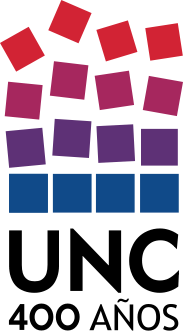
\includegraphics[height=1.7cm]{imagenes/400-anios.png} \hspace{3mm}
	
\includegraphics[height=1.22cm]{imagenes/logo-reforma.png} \hspace{3mm}	
	
\includegraphics[height=1.2cm]{imagenes/logo.jpg} 
        
\includegraphics[height=1.2cm]{imagenes/fcefyn.png}
        
\includegraphics[height=1.2cm]{imagenes/dpto-aero-logo.jpg}
                   }


\fancyfoot[LE,RO]{\small
                    P\'agina \thepage \ de \pageref{LastPage}
 }

\fancyfoot[RE,LO]{\small
  A\~no 2024. Versi\'on 01.A
}



\makeglossaries
%-----------------------------------------------------------
%		IyA. Glosario
%		2020.07.14
%
%-----------------------------------------------------------

%\section{Glosario}

%-----------------------construccion glosario--------%

%\makeglossaries

%ATM
\newglossaryentry{ATM}{ name=ATM , description={
El Sistema ATM (Gestión de Tránsito Aéreo, en inglés Air Traffic Management) consiste en la provisión de servicios que  incluyan el espacio aéreo, los aeródromos, las aeronaves, la infraestructura tecnológica y los recursos humanos.
}
}


%Graticula
\newglossaryentry{graticula}{ name=grat{\'i}cula , description={
Una grat\'icula es una red de líneas geográficas. Se utiliza esta palabra para referirse a una zona geográfica rectangular, la cual abarca 1º$\times$1º de latitud y longitud. 
}
}

%Latitud
\newglossaryentry{latitud}{ name=Latitud, description={
	Es la distancia angular entre el ecuador y un punto determinado del planeta. La latitud se mide en grados (º), entre 0 y 90; y puede representarse de dos formas:
  \begin{itemize}
\item  indicando a qu\'e hemisferio pertenece la coordenada (norte o sur); 
\item  valores positivos -norte- y negativos -sur-;
  \end{itemize}
as\'i, diez grados en latitud norte podr\'ia representarse 10ºN o 10º; y diez grados sur podr\'ia ser 10ºS o -10º.
En la navegaci\'on mar\'itima la latitud se representa con la letra griega $\phi$.
	}
	 }

%StatuteMile
\newglossaryentry{statutemile}{ name=Milla estatutaria, description={Llamada simplemente milla, se sigue usando en los países anglosajones y equivale exactamente a 1,609344 km. En inglés se llama statute mile. En los países que utilizan el sistema métrico, la milla aparece normalmente en la escala de los mapas a fin de que éstos puedan ser estudiados también por los anglosajones. De la misma forma, los países anglosajones van incorporando paulatinamente el kil\'ometro como dato adicional en su cartografía. Tiene las siguientes conversiones:
$0.3333$ leguas = $1.609344$ km = 1760 yardas = 5280 pies
}
}

%NauticalMile
\newglossaryentry{nauticalmile}{ name=Milla n{\'a}utica, description={
	Se introdujo en la náutica hace siglos, y fue adoptada (con muy ligeras variaciones) por todos los países occidentales, siendo definida como la longitud de un arco de 1' de meridiano terrestre. Una milla náutica equivale a 1852 m. Su uso está admitido en el Sistema Internacional (SI).
}
}

%Nudo
\newglossaryentry{nudo}{ name=Nudo, description={
	es una medida de velocidad utilizada tanto para navegación marítima como aérea. Equivale a una milla náutica por hora. También se utiliza en meteorología para medir la velocidad de los vientos. Aunque no existe un símbolo acordado a nivel internacional, tanto la International Hydrographic Organization (IHO) como la Oficina Internacional de Pesas y Medidas (BIPM) recomiendan kn. No obstante, a veces se utilizan kt (knot) para el singular (símbolo de kilotonelada) y kts para el plural.
}
}

%Actitud
\newglossaryentry{actitud}{name=Actitud, description={
 Respecto a una aeronave se define como los \'angulos que su nariz y alas forman con la referencia que es el horizonte. De esa manera hablamos de actitud nariz arriba, ala izquierda abajo, etc.
}
}

%Longitud
\newglossaryentry{longitud}{ name=Longitud, description={
Expresa la distancia angular entre un punto dado de la superficie terrestre y el meridiano que se tome como 0º; habitualmente en la actualidad el meridiano de Greenwich (observatorio de Greenwich), pero antiguamente hubo muchos otros que serv\'ian como referencia (para el mapa de Ptolomeo el meridiano de Alejandr\'ia, para los mapas espa\~noles hasta el siglo XIX el meridiano de C\'adiz (observatorio de C\'adiz) o el meridiano de Salamanca (observatorio de la Universidad de Salamanca, utilizado por la Compa\~n\'ia de Jes\'us), para los franceses el meridiano de Par\'is (observatorio de Par\'is), etc.).
La longitud geogr\'afica se mide en grados (º). Existen varias maneras de medirla y expresarla:
\begin{itemize}
\item  entre 0º y 360º, aumentando hacia el Este del meridiano 0º
\item  entre 0º y 180º indicando a qu\'e hemisferio pertenece
\item entre 0º y   180º positivos Este o negativos Oeste;
\end{itemize}
As\'i, noventa grados longitud este puede representarse 90º o 90ºE; y noventa grados Oeste puede ser 270º, 90º o -90º
En navegaci\'on mar\'itima la longitud se representa con la letra griega $\omega$.
	}
	 }

%Trayectoria
\newglossaryentry{trayectoria}{ name=Trayectoria, description={
Se define como el conjunto de puntos del espacio por los cuales pasa la aeronave durante su vuelo %(ver Figura \ref{fig:trayectoria}).
}
}

%Proyeccion Cartografica
\newglossaryentry{proyeccion-cartografica}{ 
	name=Proyecci{\'o}n cartogr{\'a}fica, 
	description={
 La representación de la superficie de referencia (esfera o elipsoide de revolución) sobre una superficie plana, sin que haya deformaciones es geométricamente imposible. Se producen deformaciones de tipo angular, lineal y superficial al representar en un plano la superficie terrestre.
En cartografía, este problema se resuelve mediante las proyecciones cartográficas.
La proyección cartográfica consiste en la correspondencia biunívoca entre los puntos de la superficie de referencia y sus transformaciones en el plano, llamado plano de proyección con deformaciones controladas% , ver Figura \ref{fig:proyecciones.cartograficas}.
%  \begin{figure}[!h]
%   \centering
%   \subfigure[Concepto de proyecci\'on]{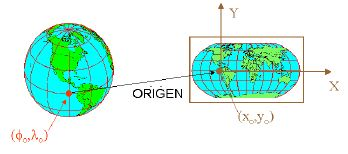
\includegraphics[width=\textwidth]{06.radionavegacion/Imagenes/transformacion.JPG}}
%   \subfigure[Tipos de proyecciones]{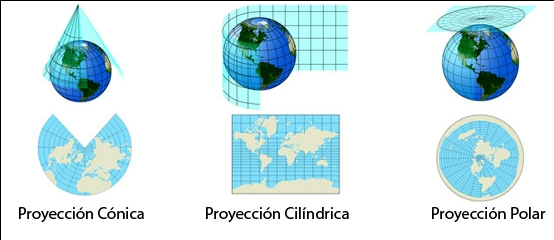
\includegraphics[width=\textwidth]{06.radionavegacion/Imagenes/proyecciones}}
%   \caption{Proyecciones cartogr\'aficas}
%   \label{fig:proyecciones.cartograficas}
% \end{figure}
}
}

%\begin{description}


% \item [Longitud] Expresa la distancia angular entre un punto dado de la superficie terrestre y el meridiano que se tome como 0º; habitualmente en la actualidad el meridiano de Greenwich (observatorio de Greenwich), pero antiguamente hubo muchos otros que serv\'ian como referencia (para el mapa de Ptolomeo el meridiano de Alejandr\'ia, para los mapas espa\~noles hasta el siglo XIX el meridiano de C\'adiz -observatorio de C\'adiz- o el meridiano de Salamanca -observatorio de la Universidad de Salamanca, utilizado por la Compa\~n\'ia de Jes\'us-, para los franceses el meridiano de Par\'is -observatorio de Par\'is-, etc.).
% La longitud geogr\'afica se mide en grados (º). Existen varias maneras de medirla y expresarla:

% \begin{itemize}
% \item  entre 0º y 360º, aumentando hacia el Este del meridiano 0º

% \item  entre 0º y 180º indicando a qu\'e hemisferio pertenece

% \item entre 0º y   180º positivos -Este- o negativos -Oeste-;
% \end{itemize}

% as\'i, noventa grados longitud este puede representarse 90º o 90ºE; y noventa grados Oeste puede ser 270º, 90ºO o -90º
% En navegaci\'on mar\'itima la longitud se representa con la letra griega $\omega$.

% \item [Actitud de una aeronave] Se define como los \'angulos que su nariz y alas forman con la referencia que es el horizonte. De esa manera hablamos de actitud nariz arriba, ala izquierda abajo, etc.

% \item [Marco de coordenadas de referencia] Define un punto de origen y un conjunto de ejes que parten de dicho origen con una determinada orientaci\'on. Estos ejes son los llamados ejes de coordenadas. Los marcos de referencia pueden o no ser inerciales. Se habla de un marco de referencia inercial si \'este no est\'a sujeto a aceleraciones, encontr\'andose en reposo o en movimiento traslacional uniforme. En los marcos de referencia inerciales se pueden aplicar las leyes de la mec\'anica de Newton.

% \item [Posici\'on] Es el conjunto de coordenadas que identifica a un punto dado en un marco de coordenadas espec\'ifico. El proceso para hallar la posici\'on a menudo es llamado posicionamiento.

% \item [Enrutamiento] Se denomina as\'i al proceso de planificar la ruta adecuada para llegar al destino.

% \item [Guiado] Este es el procedimiento para que un veh\'iculo siga por la ruta predefinida.

% \item [Trayectoria] Se define como el conjunto de puntos del espacio por los cuales pasa la aeronave durante su vuelo (ver Figura \ref{fig:trayectoria}).

% \item [Ruta] Es la curva resultante de proyectar la trayectoria sobre la superficie de la Tierra (ver Figura \ref{fig:trayectoria}).

% \item [Waypoints] Son puntos conocidos a lo largo de la ruta, y a menudo resaltan por alguna raz\'on en particular (Lugares de reporte obligatorio, puntos de intersecci\'on de aerov\'ias, etc.) (ver Figura \ref{fig:trayectoria}).

% \item [Tramo] Llamado en ingl\'es ``\textit{leg}'' (pierna), se define como un segmento de ruta comprendido entre dos waypoints (ver Figura \ref{fig:trayectoria}). 

% \item [Curso deseado] Es el \'angulo entre el norte (cualquiera que se est\'e usando: magn\'etico, geogr\'afico, etc) y la l\'inea recta que une dos waypoints sucesivos en la ruta. En ingl\'es se denomina ``\textit{Desired Track}'', y se abrevia DTK (ver Figura \ref{fig:curso}).

% \item [Derrota] En n\'autica, la derrota es el trayecto que ha recorrido una embarcaci\'on desde un punto ``\textit{A}'' hasta otro punto ``\textit{B}''. En el derrotero o carta n\'autica se traza la ruta a seguir; contiene informaciones importantes para el navegante, tales como ubicaci\'on de faros, boyas, profundidad del agua, etc. En navegaci\'on a\'erea es el \'angulo entre el norte y la l\'inea tangente a la ruta (dicha tangente corresponde, por cierto, al vector velocidad de la aeronave). En ingl\'es se le llama ``\textit{Track}'' o TK (ver Figura \ref{fig:curso}).

% \item [Error transversal] El error transversal o ``\textit{Cross-Track Error}'' (XTE) es la distancia perpendicular entre la posici\'on de la aeronave y la l\'inea que representa al curso deseado. \footnote{Es conveniente tener en cuenta que la diferencia entre el curso deseado (DTK) y la ruta realmente seguida (TK) por lo general es producida por factores externos tales como el viento cruzado (en el caso de las aeronaves) o las corrientes marinas (si se habla de barcos).}

% \item [Rumbo] El rumbo o ``Heading'' (HDG) es el \'angulo entre el norte y el eje longitudinal de la aeronave (hacia donde apunta su nariz). No coincide necesariamente con el vector velocidad (Track) dado que es posible, por ejemplo, que el piloto modifique el rumbo para contrarestar un viento cruzado (ver Figura \ref{fig:curso}).

% \item [Marcaci\'on] Se define como el \'angulo entre el norte y la l\'inea recta que une a un punto de referencia dado con la aeronave. A menudo, el punto de referencia coincide con alguna instalaci\'on importante en tierra tal como una radioayuda. En ingl\'es se le llama ``\textit{Bearing}''. Notese que el ``\textit{bearing}'' depender\'a siempre del punto que se est\'e tomando como referencia (ver Figura \ref{fig:curso}). 

% \item [ETE] ``\textit{Estimated Time En-route}'', es el intervalo de tiempo estimado que tardar\'a la aeronave en su ruta desde el punto de origen hasta el punto de destino.

% \item [ETA] ``\textit{Estimated Time of Arrival}'', es la hora estimada en que la aeronave llegar\'a a su punto de destino propuesto. 

% \item [Norte] El aparentemente simple concepto de ``\textit{Norte}'' engloba una serie de definiciones que es necesario conocer y diferenciar adecuadamente: 

%    \begin{description}
%      \item [Norte geogr\'afico] Es el que viene dado por la intersecci\'on del eje de rotaci\'on de la Tierra con la superficie de la misma 1.1. Es llamado tambi\'en ``\textit{Norte verdadero}'', y en \'el confluyen todos los meridianos.

% \item [Norte magn\'etico] Es el punto donde la mayor parte de las l\'ineas de fuerza del campo magn\'etico terrestre entran en la superficie. Se puede detectar utilizando instrumentos tales como la br\'ujula y la ``\textit{flux valve}'' (equivalente a la br\'ujula en las aeronaves modernas).

% Es importante hacer notar que el norte geogr\'afico y el magn\'etico \textbf{NO} coinciden, y que adem\'as el norte magn\'etico cambia su posici\'on con el tiempo.

% \item [Declinaci\'on magn\'etica] es el \'angulo de desviaci\'on entre las posiciones del norte magn\'etico y geogr\'afico, vistas desde un punto en particular. Se denota como D y se considera positiva cuando el \'angulo medido est\'a hacia el Este del norte verdadero, y negativo en caso contrario (ver Figura \ref{fig:declinacion-magnetica}). 

% \item [L\'ineas is\'ogonas] Se llaman as\'i a las l\'ineas que, sobre las cartas de navegaci\'on o los mapas, unen puntos que tienen la misma declinaci\'on magn\'etica. Son tambi\'en denominadas l\'ineas isog\'onicas. Adicionalmente, si una l\'inea corresponde a puntos con declinaci\'on 0º, se habla de l\'inea ag\'onica. En la Figura \ref{fig:declinacion-magnetica-anio-2000} se presenta un mapa mundial con los valores de la declinaci\'on magn\'etica para el a\~no 2000.

% \item [Norte de la Br\'ujula] Es el norte magn\'etico tal y como lo indica a bordo el instrumento adecuado (br\'ujula o flux valve). No indica realmente el norte magn\'etico pues el instrumento comete errores por diversas razones (presencia de masas met\'alicas cercanas, l\'ineas de campo magn\'etico que no son horizontales, etc).

% \item [Desviaci\'on magn\'etica] Es el error angular cometido por la br\'ujula o flux valve. El fabricante de la aeronave puede corregirla hasta cierto punto. En la Figura \ref{fig:declinacion-desviacion} se presenta la relaci\'on entre los nortes geogr\'afico, magn\'etico y de la br\'ujula con sus correspondientes diferencias angulares. 

% \item [Norte de la Cuadr\'icula] Cuando se navega a grandes latitudes (muy al norte o muy al sur del planeta), no tiene sentido guiarse por el norte magn\'etico debido, entre otras cosas, a las grandes declinaciones implicadas. Es por ello que se define arbitrariamente el Norte de la Cuadr\'icula como el norte indicado por los meridianos de la carta de navegaci\'on que se est\'a usando para navegar. 

%    \end{description}

% \item [Navegaci\'on por estima] Llamada en ingl\'es \textit{dead reckoning}, representa el proceso mediante el cual, a partir de una posici\'on previa bien conocida (llamada fix), y estimando el vector velocidad de la aeronave y el tiempo transcurrido, se obtiene (por integraci\'on en funci\'on del tiempo) la posici\'on actual de la aeronave (ver Figura \ref{fig:dead-reckoning}). 

% \end{description}





%****** Acronyms and abbreviations in avionics ******
%***** [edit] A *****

\DeclareAcronym{2D}{
	short = 2D,
	long  = Latitud y Longitud }

%2D : Latitud y Longitud

\DeclareAcronym{3D}{
	short = 3D,
	long  = Latitud\, Longitud y Altitud}
%3D : Latitud, Longitud y Altitud



% \acrodef{AGPL}{Affero General Public License}
% AGPL: Affero General Public License.
\DeclareAcronym{A/A}{
	short = A/A,
	long  = Air to Air
}

\DeclareAcronym{A/S}{
	short = A/S,
	long  = Air to Surface
}



%     * ACARS: Aircraft Communications Addressing and Reporting System
\DeclareAcronym{ACARS}{
  short = ACARS ,
  long  = Aircraft Communications Addressing and Reporting System
}

%     * ACAS: Airborne Collision Avoidance System
%     * ACP: Audio control panel
%     * ACS: Audio control system

%     * ADC: Air data computer
\DeclareAcronym{ADC}{
        short = ADC,
        long  = Air Data Computer
}

%     * ABAS: Aircraft-based augmentation system
\DeclareAcronym{ACFT}{
	short = ACFT,
	long  = Aircraft
}

%     * ADF: Automatic direction finder
\DeclareAcronym{ADF}{
	short = ADF,
	long  = {Buscador Autom\'atico de Direcci\'on, Automatic Direction Finder} 
}

%     * ADI: Attitude director indicator
\DeclareAcronym{ADI}{
	short = ADI,
	long  = Attitude Director Indicator
}

%     * ADIRS: Air Data Inertial Reference System
%     * ADIRU: Air data inertial reference unit
%     * ADM: Air data module
%     * ADS: Either; Automatic Dependent Surveillance or air data system
%     * ADS-A: Automatic Dependent Surveillance-Address
%     * ADS-B: Automatic Dependent Surveillance-Broadcast
\DeclareAcronym{ADPCM}{
	short = ADPCM,
	long  = {Modulación por codificación de impulsos diferencial adaptativa, Adaptive Differential     Pulse Code Modulation}
}

%     * AFCS: Automatic flight control system
\DeclareAcronym{AFCS}{
	short = AFCS,
	long  = Automatic Flight Control System
}
%     * AFD: Autopilot flight director
%     * AFDC: Autopilot flight director computer
%     * AFDS: Autopilot flight director system
%     * AFIS: Either; Automatic flight information service or airborne flight
%       information system
%     * AGACS: Automatic ground–air communications system, is also known as ATCSS
%       or data link
%     * AGDL: Air-Ground Data Link
%     * AGC: Automatic gain control
\DeclareAcronym{AGL}{
	short = AGL,
	long = Above Ground Level}

%     * AHC: Attitude heading control
%     * AHRS: Attitude and Heading Reference Systems
\DeclareAcronym{AHRS}{
	short = AHRS,
	long  = Attitude and Heading Reference Systems }

%     * ADAHRS: Air data and attitude heading reference system
\DeclareAcronym{ADAHRS}{
	short = ADAHRS,
	long  = Air Data and Attitude Heading Reference System}


\DeclareAcronym{AI}{
	short = AI,
	long  = Attitude Indicator}

\DeclareAcronym{AIDS}{
short = AIDS, 
long = Aircraft Integrated Data System}
%       AIDS: Aircraft Integrated Data System

%     * ALC: Automatic level control
%     * ALT: Either; altimeter or altitude
%     * ALT Hold: altitude hold mode
%     * ALTS: Altitude select
\DeclareAcronym{AM}{
	short = AM,
	long  = Amplitud Modulada}
%     * AMLCD: Active-matrix liquid crystal display
\DeclareAcronym{ANAC}{
	short = ANAC,
	long  = Agencia Nacional de Aviaci\'on Civil
}

%     * ANC: Active noise cancellation
%     * ANN: Annunciator – caution warning system normally containing visual and
%       audio alerts to the pilot
%     * ANR: Active noise reduction
%     * ANT: Antenna
%     * A/P: Autopilot
%     * APC: Autopilot computer
%     * APS: Autopilot system
%     * APU: Auxiliary power unit
% \acrodef{ARINC}{Aeronautical Radio INCorporated}
% 	ARINC: Aeronautical Radio INCorporated 
\DeclareAcronym{ARINC}{
  short = ARINC ,
  long  = Aeronautical Radio INCorporated
}

%     * ASD: Aircraft situation display
%     * ASDL: Aeronautical satellite data link
\DeclareAcronym{ASI}{
	short = ASI,
	long  = Air Speed Indicator}

\DeclareAcronym{ASK}{
	short = ASK,
	long  = { Modulación Digital por cambio de Amplitud, Amplitud Shift Keying} 
}

%     * ASR: Airport surveillance radar
%     * ASU: Avionics switching unit
%\acrodef{ATC}{Air traffic control} ATC: Air traffic control

\DeclareAcronym{ATC}{
  short = ATC ,
  long  = Air Traffic Control,
  extra = {El Control del Tráfico Aéreo, es un servicio proporcionado por controladores situados en tierra, que guían a las aeronaves en los espacios aéreos controlados y ofrecen información y apoyo a los pilotos en los Espacios Aéreos No Controlados. Tiene como objetivos  proporcionar seguridad, orden y eficiencia al tráfico aéreo. }
}

%     * ATCRBS: Air Traffic Control Radar Beacon System
%     * ATCSS: Air traffic control signaling system
%     * ATI: Unit of measure for instrument size, a standard 3¨û cutout is a 3ATI
\DeclareAcronym{ATM}{
	short = ATM ,
	long = {Gestión de Tráfico Aéreo, Air Traffic Management},
	extra = { El Sistema ATM consiste en la provisión de servicios que  incluyan el espacio aéreo, los aeródromos, las aeronaves, la infraestructura tecnológica y los recursos humanos.}
}

\DeclareAcronym{ATN}{
	short = ATN,
	long  = { Aeronautical Telecomunications Network },
}

\DeclareAcronym{ATSU}{
short = ATSU, 
long = Air Traffic Services Unit}
% 	ATSU: Air Traffic Services Unit%, implementada por AIRBUS en sus aviones (no en los A300/310), 
%		realiza las funciones generalmente usuales en unidades de gesti\'on de comunicaciones
%		de otro tipo de aviones.

%     * Avionics: Aviation + electronics
%     * AWG: American wire gauge


% ***** [edit] B *****
%     * B RNAV: Basic area navigation
%     * BARO: Barometric indication, setting or pressure
%     * BCRS: Back course
%     * BDI: Bearing distance indicator
%     * BGAN: Broadcast Global Area Network
\DeclareAcronym{Bit}{
  short = Bit ,
  long  = BInary Digit,
  extra = {Es una expresión inglesa que significa ``dígito binario''. El concepto se utiliza en la informática para nombrar a una unidad de medida de información que equivale a la selección entre dos alternativas que tienen el mismo grado de probabilidad. Un bit puede tener valor cero o uno.}
}


% ***** [edit] C *****
%     * CAI: Caution annunciator indicator
%     * CAT I: Operational performance Category 1
%     * CAT I Enhanced Allows for lower minimums than CAT I in some cases to CAT
%       2 minimums
%     * CAT II: Operational performance Category II
%     * CAT IIIa: Operational performance Category IIIa
%     * CAT IIIb: Operational performance Category IIIb
%     * CAT IIIc: Operational performance Category IIIc

\DeclareAcronym{CAMU}{
	short = CAMU,
	long  = Communications and Audio Management Unit
}

%     * CODEC: Coder/decoder
%     * CDI: Course deviation indicator
%     * CDTI: Cockpit display of traffic information

\DeclareAcronym{CFDS}{
short = CFDS, 
long = Centralised Fault Display System}
% 	CFDS: Centralised Fault Display System

%     * CFIT: Controlled flight into terrain

\DeclareAcronym{CFR}{
short = CFR, 
long = Code of Federal Regulations
}

\DeclareAcronym{CDFA}{
short = CDFA,
long = Continuous Descent Final Approach, 
extra = {OACI.
Doc 8168. 
Procedures for air navigation services.
Aircraft Operations.
Volume I - Flight Procedures
Sixth Edition, 2018.
A technique, consistent with stabilized approach procedures, for flying
the final approach segment of a non-precision instrument approach procedure as a continuous descent, without
level-off, from an altitude/height at or above the final approach fix altitude/height to a point approximately 15 m
(50 ft) above the landing runway threshold or the point where the flare manoeuvre should begin for the type of
aircraft flown.}
}



\DeclareAcronym{CDU}{
    short = CDU, 
    long = Control Display Unit
    }   
% 	CDU: Control Display Unit

%     * COMM or COM: Communications receiver
\DeclareAcronym{COMM}{
	short = COMM,
	long  = CoMMunications receiver
}





\DeclareAcronym{COTS}{
	short = COTS,
	long  = Commercial-Off-The-Shelf
}


%     * CNS: Communication, navigation, surveillance
%     * CNS/ATM: Communication, navigation, surveillance/air traffic Management
%       [1]
%     * CPDLC: Controller–pilot data link communications
%     * CPS: Cycles per second
%     * CRT: Cathode ray tube
\DeclareAcronym{CRT}{
	short = CRT,
	long  = Cathode Ray Tube
}

%     * CTAF: Common traffic advisory frequency
%     * CV/DFDR: Cockpit voice and digital flight data recorder
%     * CVR: Cockpit voice recorder
%     * CWS: Control wheel steering

% ***** [edit] D *****
%     * DA: Drift angle
%     * DAPs: Downlink of aircraft parameters
%     * DCDU: Data link control and display unit
%     * DG: Directional gyroscope
\DeclareAcronym{DG}{
	short = DG,
	long  = Directional Gyroscope}

%     * DGPS: Differential global positioning system
%     * DH: Decision height

% \acrodef{DITS}{Digital Information Transfer System}
\DeclareAcronym{DITS}{
  short = DITS ,
  long  = Digital Information Transfer System
%  extra = {El Control del Tráfico Aéreo, es un servicio proporcionado por controladores situados en tierra, que guían a las aeronaves en los espacios aéreos controlados y ofrecen información y apoyo a los pilotos en los Espacios Aéreos No Controlados. Tiene como objetivos  proporcionar seguridad, orden y eficiencia al tráfico aéreo. }
}

% 	DITS: Digital Information Transfer System
%     * DLR: Data link recorder
%     * DME: Distance measuring equipment
\DeclareAcronym{DME}{
	short = DME,
	long  = Display Measuring Equipment
}

\DeclareAcronym{DMC}{
	short = DMC,
	long  = Display Management Computers
}
%     * DNC: Direct noise canceling
%     * DP: Departure procedures
\DeclareAcronym{DPCM}{
	short = DPCM,
	long  = {Modulación de Pulsos Codificados Diferenciales, Differential Pulse Code Modulation}
}

%     * DSP: Digital signal processing
%     * DUAT: Direct user access terminal

\DeclareAcronym{DVI}{
	short = DVI ,
	long = Direct Voice Input
}

% ***** [edit] E *****
%     * EADI: Electronic attitude director indicator
\DeclareAcronym{ECAM}{
	short = ECAM, 
	long  = Electronic Centralized Aircraft Monitor
}

% \acrodef{EFD}{Electronic flight display}
\DeclareAcronym{EFD}{
	short = EFD,
	long  = Electronic Flight Display
}

%     * EFIS: Electronic flight instrument system
\DeclareAcronym{EFIS}{
	short = EFIS,
	long  = Electronic Flight Instrument System
}

\DeclareAcronym{EFVS}{
	short = EFVS,
	long  = Enhanced Flight Vision Systems}


%     * EGPWS: Enhanced ground proximity warning system
%     * EGT: Exhaust gas temperature
\DeclareAcronym{EGT}{
	short = EGT,
	long  = Exhaust Gas Temperature}

%     * EHS: Enhanced surveillance
%     * EHSI: Electronic horizontal situation indicator
%       EICAS: Engine indication crew alerting system
\DeclareAcronym{EICAS}{
	short = EICAS,
	long  = Engine Indication Crew Alerting System
}

\DeclareAcronym{EIS}{
	short = EIS,
	long  = Electronic Instrument System
}

%     * ELT: Emergency locator transmitter
%     * ENC: Electronic noise canceling
%     * ENG: Engine
%     * ENR: Electronic noise reduction
%     * EPR: Engine pressure ratio
%     * ETOP: Extended-range twin-engine operation
\DeclareAcronym{ETOP}{
	short = ETOP,
	long  = Extended-Range Twin-Engine Operation
}

\DeclareAcronym{EWD}{
	short = EWD,
	long  = Engine Warning Display}

% ***** [edit] F *****
%     * FADEC: Full authority digital engine control
%     * FANS: Future Air Navigation System
%     * FAT: Free air temperature
%     * FDPS: Flight plan Data Processing System
%     * FDRS: Flight data recorder system
\DeclareAcronym{FDS}{
	short = FDS,
	long  = Flight Director System }

%     * FDU: Flux detector unit
%     * FF: Fuel flow
%FIR: Flight Information Region
\DeclareAcronym{FIR}{
	short = FIR,
	long  = Flight Information Region 
}

%     * FIS-B: Flight information services – broadcast
%     * FLIR: Forward-looking infra-red
%     * FLTA: Forward-looking terrain avoidance

\DeclareAcronym{FM}{
	short = FM,
	long  = Frecuencia Modulada}

% \acrodef{FMC}{Flight Management Computer}
% 	FMC: Flight Management Computer
\DeclareAcronym{FMC}{
	short = FMC,
	long  = Flight Management Computer
}

% \acrodef{FMGS}{Flight Management Guidance System}
% 	FMGS: Flight Management Guidance System
\DeclareAcronym{FMGS}{
	short = FMGS,
	long  = Flight Management Guidance System
}

%       FMS: Flight Management System
\DeclareAcronym{FMS}{
	short = FMS,
	long  = Flight Management System
}
%     * FREQ: Frequency
%     * FSS: Flight service station
\DeclareAcronym{FWC}{
	short = FWC,
	long  = Flight Warning Computer
}

\DeclareAcronym{FSK}{
	short = FSK,
	long  = {Modulación Digital por cambio de Frecuencia, Frecuency Shift Keying} }

%     * FWS: Flight warning system
%     * FYDS: Flight director/ Yaw damper system

% ***** [edit] G *****
\DeclareAcronym{GBAS}{
short = GBAS,
long = Ground based augmentation system,
extra = {\href{https://www.skybrary.aero/sites/default/files/bookshelf/3844.pdf}{GBAS quick facts.}}
}

%     * GCAS: Ground collision avoidance system
%     * GCU: Generator control unit
%     * GDOP: Geometric dilution of precision
%     * GGS: Global positioning system ground station
%     * GHz: Gigahertz
%     * GLNS: GPS Landing and Navigation System
%     * GLNU: GPS landing and navigation unit

\DeclareAcronym{GLONASS}{
	short = GLONASS,
	long  = Global NAvigation Satellite System
}

\DeclareAcronym{GLS}{
short = GLS,
long =  GBAS Landing System
}
%     * GLU: GPS landing unit

% 	GND: Ground (tierra)


    % * GNSS: Global Navigation Satellite System
\DeclareAcronym{GNSS}{
	short = GNSS,
	long  = Global Navigation Satellite System}

    % * GMT: Greenwich Mean Time

%     GPS: Global Positioning Satellite or Global Positioning System
\DeclareAcronym{GPS}{
	short = GPS,
	long  = Global Positioning Satellite o Global Positioning System
}

    % * GPWC: Ground proximity warning computer
%      GPWS: Ground proximity warning system
\DeclareAcronym{GRI}{
	short = GRI,
	long  = Group Repetition Interval.
}


% ***** [edit] H *****
%     * HDG: Heading
%     * HDG SEL: Heading select
%     * HDOP: Horizontal dilution of precision
%     * HF: High frequency
\DeclareAcronym{HF}{
	short = HF,
	long  = High Frequency
}

%     * HHLD: Heading hold
\DeclareAcronym{HI}{
	short = HI,
	long  = Heading Indicator}
%     * HSD: High-speed data
%     * HSI: Horizontal situation indicator
\DeclareAcronym{HSI}{
        short = HSI,
        long  = Horizontal Situation Indicator
}

%     * HSL: Heading select
%     * HUD: Head-up display
\DeclareAcronym{HUD}{
	short = HUD,
	long  = Head-Up Display
}
%     * HMD: Helmet-mounted display
\DeclareAcronym{HMD}{
	short = HMD,
	long  = Helmet-Mounted Display}

% ***** [edit] I *****
\DeclareAcronym{IAC}{
	short = IAC,
	long  = Instrumental Approach Charts}
%IAC: Instrumental Approach Charts


%     * IAS: Indicated airspeed
%     * ID: Identify/Identification or identifier
%     * IDENT: Identify/identifier
%     * IDS: Information display system or integrated display system
%     * IFE: In-flight entertainment
%     * IFR: Instrument flight Rules
\DeclareAcronym{IFR}{
	short = IFR,
	long  = Instrument Flight Rules
}

%     * ILS: Instrument landing system
\DeclareAcronym{ILS}{
	short = ILS,
	long  = Instrument Landing System
}

\DeclareAcronym{IMA}{
	short = IMA,
	long  = Integrated Modular Avionics,
	extra = {
El concepto de aviónica modular integrada intenta reducir la variedad de LRU diseñando la aviónica con componentes comunes. Por ejemplo un tipo de fuente de alimentación, un tipo de unidad de memoria, un tipo de placa de procesamiento y solo algunas variaciones de módulos de entrada / salida. Esto reduce la cantidad de piezas de repuesto necesarias que se deben mantener en stock. Las LRU de IMA tienen funciones más genéricas que en un sistema de aviónica tradicional.
%The Integrated Modular Avionics concept attempts to reduce the variety of LRU's by designing the avionics with common components. E.g. one type of power supply, one type of memory unit, one type of processing board and only a few variations of input/output modules. This reduces the number of replacement parts needed to be kept on stock. The LRUs of IMA have more generic functions than in a traditional avionics system.
}
}

\DeclareAcronym{IMU}{
	short = IMU,
	long  = Inertial Measurement Unit
}

%     * IMC: Instrument meteorological conditions
\DeclareAcronym{IMC}{
	short = IMC,
	long  = Instrument Meteorological Conditions}

%     * InHg: Inch of Mercury
%     * IND: Indicator[disambiguation needed]
%     * INS: Inertial Navigation System
\DeclareAcronym{INS}{
	short = INS,
	long  = Inertial Navigation System
}


%     * ISA: International Standard Atmosphere
%     * ISP: Integrated switching panel
%     * ITT: Interstage turbine temperature
%     * IVSI: Instantaneous vertical speed indicator

% ***** [edit] J *****
%     * JTIDS: Joint Tactical Information Distribution System

% ***** [edit] L *****
%     * LAAS: Local Area Augmentation System
%     * LADGPS: Local Area Differential GPS
%     * LCD: Liquid crystal display
\DeclareAcronym{LCD}{
	short = LCD,
	long  = Liquid Crystal Display
}

%     * LDGPS: Local area differential global positioning satellite
%     * LED: Light-emitting diode
\DeclareAcronym{LED}{
	short = LED,
	long  = Light-Emitting Diode
}

%     * LMM: Locator middle marker
%     * LOC: Localizer
%     * LOM: Locator outer marker
%     * LORAN: Long-range navigation
\DeclareAcronym{LORAN}{
	short = LORAN,
	long  = Long-Range Navigation
}

\DeclareAcronym{LOS}{
  short = LOS ,
  long  = Line-Of-Sight 
}


%     * LRU: Line-replaceable unit
\DeclareAcronym{LRU}{
	short = LRU,
	long  = Line Replaceable Unit,
	extra = { Una LRU es una pieza de hardware que se puede cambiar por una pieza de repuesto en un tiempo relativamente corto abriendo y cerrando sujetadores y conectores. El término LRU se emplea en aviónica pero también en hardware ATC. Ejemplos de esto son FMC, transpondedor, etc.
Cuando se tiene un sistema de aviónica complejo se suele terminar con una gran variedad de LRUs, las cuales tienen una función muy específica. Como desventaja, para poder reemplazar rápidamente las piezas defectuosas, el personal de mantenimiento necesita un gran stock de repuestos.
}
}

\DeclareAcronym{LSB}{
	short = LSB,
	long  = Least Significant Bit
}

\DeclareAcronym{LUF}{
  short = LUF ,
  long  = Lowest Usable Frecuency 
}

\DeclareAcronym{LVT}{
  short = LVT ,
  long  = Low Volume Terminal 
}


% ***** [edit] M *****
%     * MAP: Manifold absolute pressure or missed approach point
%     * MB: Marker beacon
%     * MCBF: Mean cycles between failures

\DeclareAcronym{MCDU}{
short = MCDU, 
long = Multi Control Display Unit}
% 	MCDU: Multi Control Display Unit
%     * MDA: Minimum decent altitude
%     * MEL: Minimum equipment list

\DeclareAcronym{MEMS}{
	short = MEMS,
	long  = MicroElectroMechanical Systems}

%     * MF: Medium frequency
\DeclareAcronym{MF}{
	short = MF,
	long = {Frecuencias Medias, Medium Frequency}
}

%     * MFD: Multi-function display
\DeclareAcronym{MFD}{
	short = MFD,
	long  = Multi-Function Display
}

%     * MFDS: Multi-function display system
%     * MIC: Microphone
%     * MIDS: Multifunctional Information Distribution System
\DeclareAcronym{MIDS}{
  short = MIDS ,
  long  = Multifunctional Information Distribution System
}


%     * MILSPEC: Military specification
\DeclareAcronym{MIU}{
  short = MIU ,
  long  = Mids Interface Unit
}

%     * MKR: Marker beacon
%     * MLS: Microwave landing system
%     * MM: Middle marker
%     * MNPS: [Minimmum navigation performance specifications]
%     * MMD: Moving map display
%     * MOA: Military operations area
%     * Mode A: Transponder pulse-code reporting
%     * Mode C: Transponder code and altitude reporting
%     * Mode S: Transponder code, altitude, and TCAS reporting
%     * MOSArt: Modular Open System Architecture

\DeclareAcronym{MSB}{
	short = MSB,
	long  = Most Significant Bit
}


%     * MSG: Message
\DeclareAcronym{MSL}{
	short = MSL,
	long  = Mean Sea Level}

%     * MSP: Modes S-Specific Protocol
%     * MSSS: Mode S-Specific Services
%     * MTBF: Mean time between failures
%     * MTTF: Mean time to failure

\DeclareAcronym{MUF}{
  short = MUF ,
  long  = Maximum Usable Frecuency 
}


%     * MVFR: Marginal visual flight rules
% ***** [edit] N *****
\DeclareAcronym{NAM}{
	short = NAM,
	long  = Noise Alleviation Measures
}

\DeclareAcronym{NAP}{
short =NAP,
long = Non-Precision Approach
}

%     * NAS: National Airspace System
%     * NAV: Navigation receiver
%     * Navaid: Navigational aid
%     * NAVCOMM: Navigation and communications equipment or receiver
%     * NAVSTAR-GPS: The formal name for the space-borne or satellite navigation
%       system
%     * NCATT: National Center for Aircraft Technician Training
%     * ND: Navigation display
\DeclareAcronym{ND}{
	short = ND,
	long  = Navigation Display
}

%     * NDB: Non-directional radio beacon
\DeclareAcronym{NDB}{
	short = NDB,
	long  = {Baliza No Direccional, Non-Directional Beacon}
}

%     * NFF: No fault found
%     * NM or NMI: Nautical mile
%     * NoTAM: Notice to airmen

\DeclareAcronym{NPA}{
       short= NPA ,
       long = Non-precision approach
}
%     * NVD: Night vision device
%     * NVG: Night vision goggles

% ***** [edit] O *****
%     * OAT: Outside air temperature
%     * OBS: Omnibearing selector
%     * OM: Outer marker
% 	OLED: Organic Light-Emitting Diode
\DeclareAcronym{OLED}{
	short = OLED,
	long  = Organic Light-Emitting Diode
}

% ***** [edit] P *****
%     * PA: Public address system
%     * P-Code: GPS precision code
%     * PAPI: Precision approach path indicator
\DeclareAcronym{PAM}{
	short = PAM,
	long  = {Modulación de Pulsos en Amplitud, Pulse-Amplitude Modulation }
}

\DeclareAcronym{PBN}{
        short = PBN ,
        long  = Performance Based Navigation
}

\DeclareAcronym{PAPI}{
	short = PAPI,
	long  = Precision Approach Path Indicator
}

%     * PAR: Precision approach radar
\DeclareAcronym{PAR}{
	short = PAR,
	long  = Precision Approach Radar
}

\DeclareAcronym{PCM}{
	short = PCM,
	long  = {Modulación de Pulsos Codificados, Pulse Code Modulation}
}

%     * PD: Profile descent
%     * PDOP: Position dilution of precision
\DeclareAcronym{PDS}{
	short = PDS,
	long  = Portable Data Store
}


%     * PFD: Primary flight display or primary flight director
\DeclareAcronym{PFD}{
	short = PFD,
	long  = Primary Flight Display
}

\DeclareAcronym{PM}{
	short = PM,
	long  = {Fase Modulada, Phase Modulation}
}

%     * PMG: Permanent magnet generator
%     * PND: Primary navigation display
%     * PNR: Passive noise reduction
%     * POS: Position[disambiguation needed]
\DeclareAcronym{PPM}{
	short = PPM,
	long  = {Modulación de Pulsos de Posici\'on, Pulse Position Modulation}
}

\DeclareAcronym{PSK}{
	short = PSK,
	long  = {Modulación Digital por cambio de Fase, Phase Shift Keying}
}

\DeclareAcronym{PWM}{
	short = PWM,
	long = {Modulación por Ancho de Pulso, Pulse Wide Modulation}
}

%     * P-RNAV: precision area navigation
%     * PSR: Primary surveillance radar
%     * PTT: Push-to-talk




% ***** [edit] R *****
%     * RA: Resolution advisory (TCAS)
\DeclareAcronym{RAAC}{
	short = RAAC,
	long  = Regulaciones Argentinas de Aviaci\'on Civil
}

\DeclareAcronym{RAF}{
	short = RAF,
	long  = Royal Air Force}

%     * RAI: Radio altimeter indicator
%     * RAIM: Receiver-autonomous integrity monitoring, also remote autonomous
%       integrity monitoring
%     * RALT: Radar or radio altimeter
%     * RAT: Ram air turbine
\DeclareAcronym{RBI}{
	short = RBI,
	long  = Relative Bearing Indicator
}

%     * RCR: Reverse current relay
%     * RCVR: Receiver
%     * RDMI: Radio distance magnetic indicator
%     * RDP: Radar data processing system
%     * RDR: Radar
%     * REF: Reference
%     * REIL: Runway end identifier lights
%     * REL: Relative[disambiguation needed]
%     * RF: Radio frequency
\DeclareAcronym{RF}{
	short = RF,
	long  = Radio Frequency }


%     * RFI: Radio frequency interference
%     * RHSM: Reduced horizontal separation minimal
%     * RLG: Ring laser gyroscope
%     * RLY: Relay
%     * RMI: Radio magnetic indicator
\DeclareAcronym{RMI}{
	short = RMI,
	long  = Radio Magnetic Indicator
}

%     * R-NAV: Area navigation
%     * RNG: Range

\DeclareAcronym{RNP}{
        short = RNP,
        long = Required navigation performance
        }

%     * ROC: Rate of climb
%     * ROD: Rate of descent
%     * RPA: Remotely piloted aircraft (Unmanned aerial vehicle)
%     * RPM: Revolutions per minute
%     * RTE: Route
%     * RVR: Runway visual range
%     * RVSM: Reduced vertical separation minimum
%     * RX: Receiver

% ***** [edit] S *****
\DeclareAcronym{SBAS}{
short = SBAS,
long = Satellite Based Augmentation System,
extra = {Sistema de Aumentación Basado en Satélites, es un sistema de corrección de las señales que los Sistemas Globales de Navegación por Satélite (GNSS) transmiten al receptor GPS del usuario. Los sistemas SBAS mejoran el posicionamiento horizontal y vertical del receptor y dan información sobre la calidad de las señales. Aunque inicialmente fue desarrollado para dar una precisión mayor a la navegación aérea, cada vez se está generalizando más su uso en otro tipo de actividades que requieren de un uso sensible de la señal GPS. }
}


\DeclareAcronym{SD}{
	short = SD,
	long  = System Display
}

\DeclareAcronym{SDAC}{
	short = SDAC,
	long  = System Data Acquisition Concentrator
}
%     * SAT: Static air temperature
%     * SATCOM: Satellite communication
%     * SATNAV: Satellite navigation
%     * SD: Secure digital
%     * SELCAL: Selective calling

\DeclareAcronym{SID}{
short = SID,
long = Standard Instrument Departure
}
%       SID: Standard Instrument Departure

%     * SIU: Satellite interface unit
%     * S: Sensitivity Level
%     * SMS: Short Messaging Service
%     * SNR: Signal-to-noise ratio
%     * SPKR: Speaker
%     * SQ or SQL: Squelch
%     * SSCV/DR: Solid-state cockpit voice/data recorder
%     * SSCVR: Solid-state cockpit voice recorder
%     * SSFDR: Solid-state flight data recorder

\DeclareAcronym{SSM}{
  short = SSM ,
  long  = Sign/Status Matrix
}

%     * SSR: Secondary surveillance radar

\DeclareAcronym{STAR}{
short = STAR, 
long = Standard Terminal Arrival Route}
%       STAR: Standard Terminal Arrival Route

% \acrodef{STARS}{Standard Terminal Automation Replacement System}
\DeclareAcronym{STARS}{
short = STARS,  
long =  Standard Terminal Automation Replacement System
}



%     * STC: Supplemental Type Certificate
%     * STCA: Short-Term Conflict Alert
%     * STP: Standard temperature and pressure
\DeclareAcronym{STP}{
	short = STP,
	long = Standard Temperature and Pressure
}

%     * SUA: Special use airspace

% ***** [edit] T *****
%     * TA: Traffic advisory (see TCAS)
%     * TACAN: Tactical air navigation system
\DeclareAcronym{TACAN}{
	short = TACAN,
	long = Tactical Air Navigation System
}

%     * Tach: Tachometer
%     * TAD: Terrain awareness display
%     * TAF: Terminal area forecast
%     * TAS: True airspeed
%     * TAT: True air temperature, or total air temperature
%     * TAWS: Terrain awareness warning system
\DeclareAcronym{TAWS}{
	short = TAWS,
	long  = Terrain Awareness Warning System
}

%     * TBO: Time before overhaul, or time between overhaul
\DeclareAcronym{TC}{
	short = TC,
	long  = Turn Coordinator}

%     * TCA: Throttle control assembly, or terminal control area
%     * TCAS: Traffic collision avoidance system
%     * TCF: Terrain clearance floor
%     * TCN: TACAN
%     * TCU: TACAN control unit
%     * TDOP: Time dilution of precision
%     * TDR: Transponder (in some cases)
%     * TERPS]]: Terminal instrument procedures, or terminal enroute procedures
%     * TFR: Temporary flight restrictions
%     * TFT: Thin-film transistor
%     * TGT: Turbine gas temperature, or target
%     * THDG: True heading
%     * TIAS: True indicated airspeed
%     * TIS: Traffic information service
%     * TK: Track angle
%     * TKE: Track-angle error
%     * TLA: Three-letter acronym
%     * TOGA: Takeoff/Go-around switch, Takeoff/go-around thrust
%     * TOT: Turbine outlet temperature
%     * TR or T/R: Transmitter receiver or transceiver
%     * TRACON: Terminal radar approach control
%     * TRANS: Transmit, Transmission, or Transition[disambiguation needed]
%     * TRK: Track
%     * TRP: Mode S transponder
%     * TTR: TCAS II transmitter/receiver
%     * TTS: Time to station
%     * TVE: Total vertical error
%     * TWDL: Two-way data link, or terminal weather data link
%     * TWDR: Terminal Doppler Weather Radar
%     * TWIP: Terminal weather information for pilots
%     * TWR: Terminal weather radar
%     * TX: Transmit

% ***** [edit] U *****
%     * UART: Universal asynchronous receiver transmitter
%     * UAV: Unmanned aerial vehicle
%     * UHF: Ultra-high frequency
\DeclareAcronym{UHF}{
	short = UHF,
	long  = Ultra-High Frequency
}

%     * ULB: Underwater locator beacon
%     * USB: Universal Serial Bus
%     * UTC: Universal Time Coordinate
\DeclareAcronym{UTC}{
	short = UTC,
	long  = Universal Time Coordinate}

\DeclareAcronym{UTM}{
	short = UTM,
	long  = Universal Transverse Mercator }

% ***** [edit] V *****
%     * V: Volts or voltage
%     * VASI: Visual approach slope indicator
\DeclareAcronym{VASI}{
	short = VASI,
	long  = Visual Approach Slope Indicator 
}

%     * VDL: VHF Data Link
%     * VDR: VHF digital radio
%     * VFO: Variable frequency oscillator
%     * VFR: Visual flight rules
\DeclareAcronym{VFR}{
	short = VFR,
	long  = Visual Flight Rules
}

%     * VG/DG: Vertical gyroscope/directional gyroscope
%     * VGA: Video Graphics Array
%     * VHF: Very high frequency
\DeclareAcronym{VHF}{
  short = VHF ,
  long  = Very High Frecuency
}

\DeclareAcronym{VNAV}{
short = VNAV,
long = Vertical NAVigation
}



%     * V/L: VOR/Localizer
%     * VMC: Visual meteorological conditions or minimum control speed with
%       critical engine out

%     * VNE: Never exceed speed
%     * VNO: Maximum structural cruising speed
%     * VNR: VHF navigation receiver

\DeclareAcronym{VOGAD}{
	short = VOGAD,
	long  = Voice Operated Gain Adjustable Device
}

%     * VOR: VHF omnidirectional range and ranging
\DeclareAcronym{VOR}{
	short = VOR,
	long  = VHF Omnidirectional Range and Ranging }

%     * VOR/DME: VOR with Distance measuring equipment
%     * VOR/MB: VOR marker beacon
%     * VORTAC: VOR and TACAN combination

\DeclareAcronym{VOS}{
	short = VOS,
	long  = Voice Operated Switch
}

%     * VOX: Voice transmission
%     * VPATH: Vertical path
%     * V/R: Voltage regulator
%     * V/REF: Reference velocity
%     * V/S: Vertical speed
%     * VSI: Vertical speed indicator
\DeclareAcronym{VSI}{
	short = VSI,
	long  = Vertical Speed Indicator}

%     * VSM: Vertical separation limit
%     * VSO: Stall speed in landing configuration
%     * VSWR: Voltage–standing wave ratio
%     * V/TRK: Vertical track
%     * VX: Speed for best angle of climb
%     * VY: Speed for best rate of climb

% ***** [edit] W *****
%     * WAAS: Wide Area Augmentation System
%     * WD/WINDR: Wind direction
%     * WMA: WXR waveguide adapter
%     * WMI: WXR indicator mount
%     * WMS: Wide-area master station
%     * WMSC: Weather message switching center
%     * WMSCR: Weather message switching center replacement
%     * WPT: Waypoint
%     * WRT: WXR receiver transmitter
%     * WX: Weather
%     * WXR: Weather radar system
%     * WYPT: Waypoint

% ***** [edit] X *****
%     * XCVR: Transceiver
%     * XFR: Transfer
%     * XMIT: Transmit
%     * XMSN: Transmission
%     * XMTR: Transmitter
%     * XPDR: Transponder
%     * XTK: Crosstrack

% ***** [edit] Y *****
%     * YD: Yaw damper

% ***** [edit] See also *****
%     * Avionics
%     * List of aviation, aerospace and aeronautical abbreviations

% ***** [edit] References *****
%    1. ^ http://wwwicaoint/icao/en/ro/rio/execsumpdf


% Retrieved from "http://en.wikipedia.org/w/
% index.php?title=Acronyms and abbreviations in avionics&amp;oldid=518531528"
	% Archivo de acronimos


\begin{document}

\renewcommand{\listtablename}{\'Indice de tablas} 
\renewcommand{\tablename}{Tabla}  % para que figure como título Tabla en lugar de Cuadro

\renewcommand{\appendixtocname}{Ap\'endices}
\renewcommand{\appendixpagename}{Ap\'endices}

\renewcommand{\baselinestretch}{1.5}       % interlineado factor 1.5

\setlength{\parindent}{0pt}      % que la sangria sea 0 (cero)

\clearpage
\thispagestyle{fancy}

\maketitle

\tableofcontents

% Version 2024
%

\chapter*{Datos de la Asignatura}
\label{chap:00.datos.de.IyA}
  \addcontentsline{toc}{chapter}{Datos de la Asignatura}

  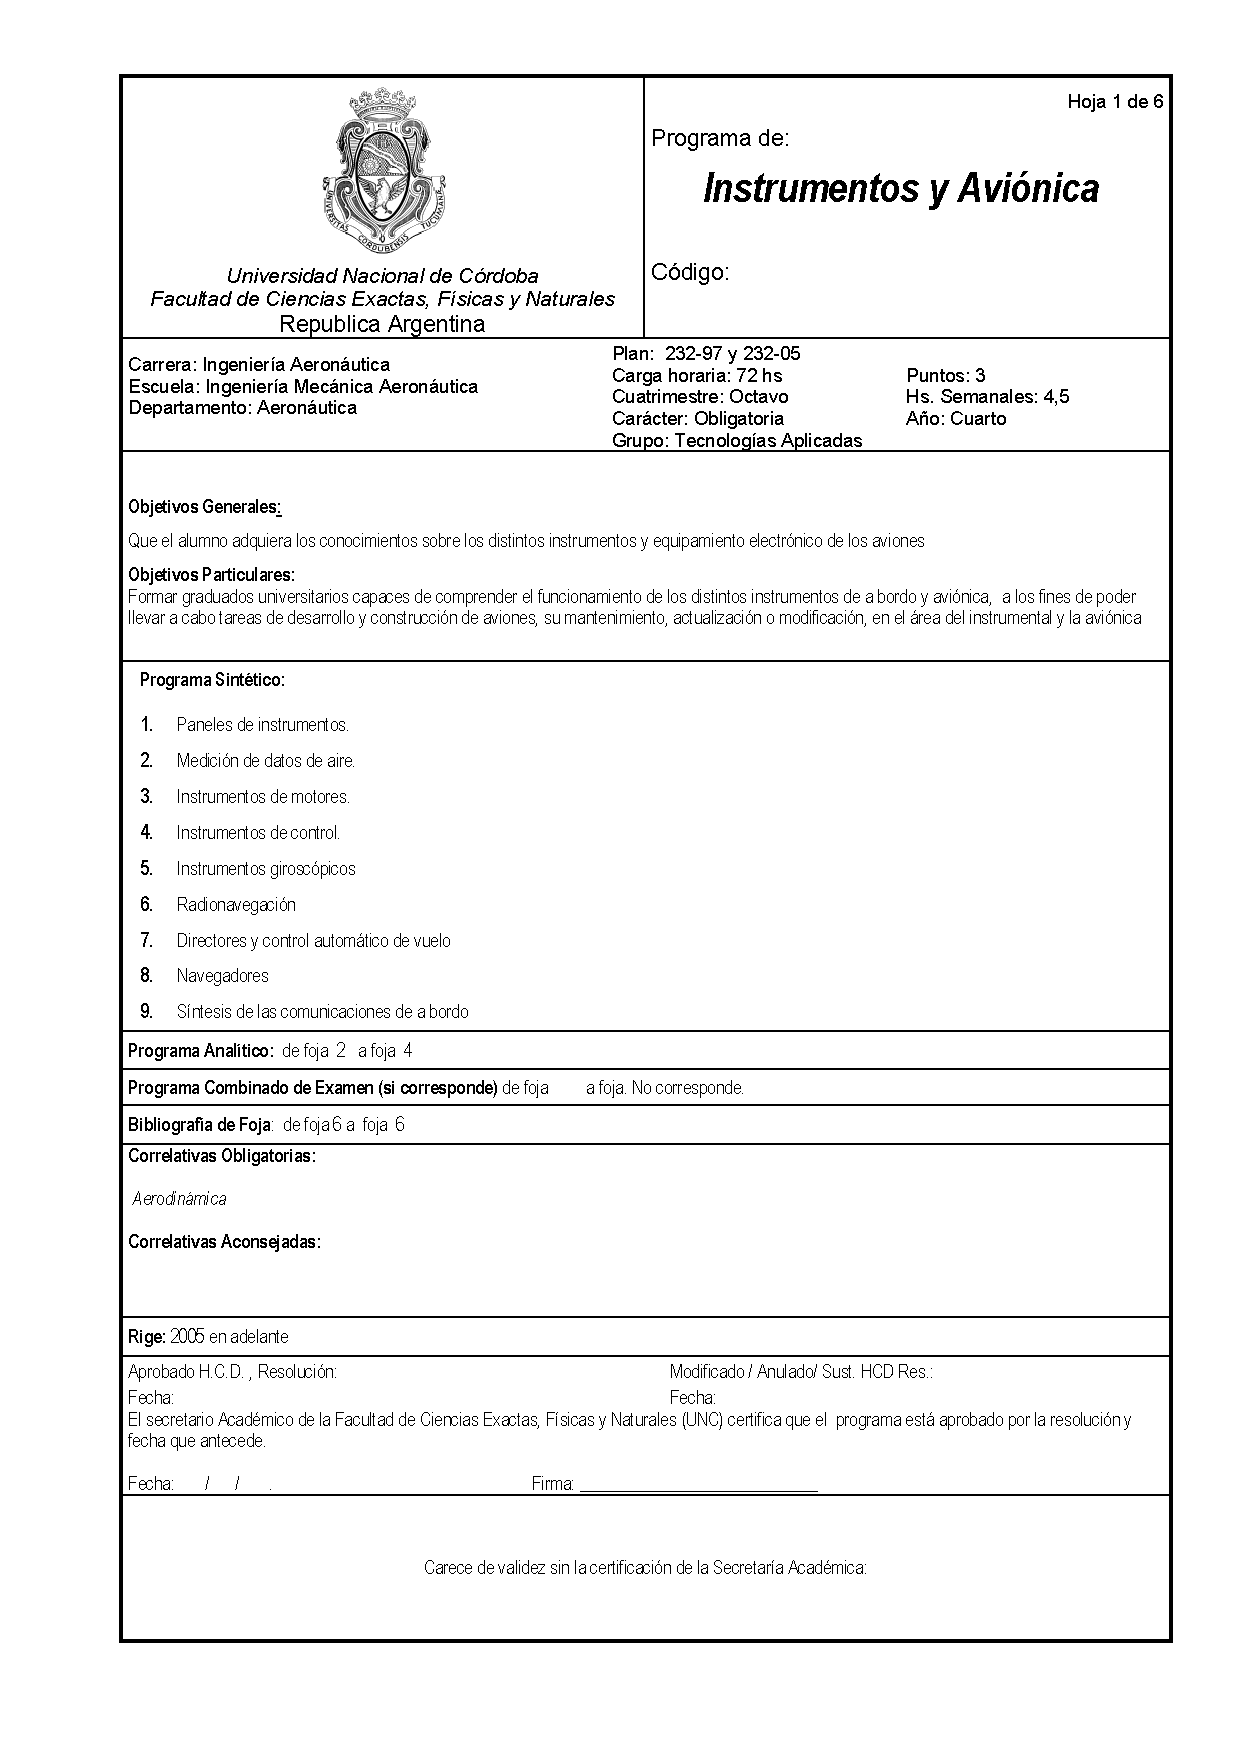
\includepdf[pages=-, fitpaper=false, scale=0.90, %landscape=true,
  offset = 0 -20,
  pagecommand={\thispagestyle{fancy}}]
  {00.Datos.IyA/Instrumentos_Y_Avionica.pdf}


\section{Días y horarios de clases}
\label{sec:dias+horarios.clases}

La asignatura se dicta de manera sincrónica/presencial en el año 2024
los días jueves de 15:45 hs a 20:15 hs.

Para las clases sincrónicas se emplea Google Meet,
 el link a la clase de la asignatura es: \\
\href{https://meet.google.com/vpm-vdau-qrq}{https://meet.google.com/vpm-vdau-qrq}
 % \url{https://classroom.google.com/c/MzY3MDEyNzQ1MjA2?cjc=wbdwdwc}

Para las clases presenciales y las evalauaciones se empleará el aula asignada a tal efecto.

El material de estudio y comunicaciones con la Cátedra se realiza a través de Google Meet cuyo link es: \\
\href{https://classroom.google.com/c/Njk3NTIwODU1Mzk4}{https://classroom.google.com/c/Njk3NTIwODU1Mzk4}



\section*{Adecuación transitoria de la metodología de cursada  y evaluación \mbox{segundo} semestre 2024}
\label{00.Adecuacion.transitoria}
  \addcontentsline{toc}{section}{Adecuación transitoria de la metodología de cursada   y evaluación  segundo semestre 2024}


\subsection*{Modalidad de enseñanza} 

Las clases se dictarán algunas de forma SINCRÓNICA y otras con PRESENCIALIDAD FÍSICA entre los docentes y los alumnos.

El día de dictado de clases será el jueves de cada semana de 15:45 a 20:

Material de estudio, asignación de tareas mediante Google Classroom


\subsection*{Modalidad de evaluación}

Las evaluaciones serán con presencialidad física de los alumnos/as.

Cantidad de parciales dos (2).

Las/los estudiantes que hayan desaprobado un (1) examen parcial teórico/práctico, si el restante examen parcial fue aprobado, tienen derecho a un (1) recuperatorio, cuya nota reemplazará a la del examen parcial reprobado.

Coloquio  tomados con presencialidad física de los alumnos/as. Cantidad uno (1).

\subsection*{Condiciones Transitorias de Regularidad}

\begin{itemize}
\item Estar correctamente matriculado para el cursado de la asignatura
\item Aprobar con nota no inferior a 4 (cuatro) cada uno de los  dos (2) exámenes parciales. 

\item Presentar y aprobar los trabajos prácticos
\end{itemize}

\subsection*{Condiciones Transitorias de Aprobación definitiva (Promoción) }


\begin{itemize}
\item Haber aprobado las correlativas previas o aprobar las que se encuentren pendientes dentro del plazo de validez de la regularidad.

\item  Estar correctamente matriculado para el cursado de la
  asignatura.
\item Aprobar con nota no inferior a 4 (cuatro) cada uno de los dos (2) exámenes parciales. 
\item Aprobar un coloquio integrador con nota no inferior a 4 (cuatro)
\item Presentar y aprobar los trabajos prácticos
\end{itemize}



\section*{Cronograma para el dictado de la Asignatura a\~no 2024}
\label{sec:00.cronograma}
  \addcontentsline{toc}{section}{Cronograma para el dictado a\~no 2024}

  \begin{itemize}
  \item Capítulo 1. Paneles de Instrumentos (GARCIA) 8/08/2024
  \item Capítulo 6. Radionavegación (OLIVA) 15/08/2024
  \item Capítulo 6. Radionavegación (GARCIA) 22/08/2024    
  \item Capítulo 9. Síntesis de las comunicaciones de a bordo (OLIVA)     29/08/2024
  \item \textbf{Parcial 01,  05/9/2024 Abarca Capítulos 1, 6, 9.  PRESENCIAL}

  \item Capítulo 8. Navegadores (SORIA) 12/9/2024 {\bf CLASE PRESENCIAL}
  \item Capítulo 8. Navegadores (GPS, nav. inerc.) (GIRAUDO) 19/9/2024    
    
  \item Capítulo 7. Directores y control automático de vuelo ( SORIA) 26/09/2024  {\bf CLASE PRESENCIAL}
  
    \item Capítulo 4. Instrumentos de control. 
          Capítulo 3. Instrumentos de motores (GIRAUDO) 03/10/2024
  
  \item Capítulo 2. Medición de datos de aire (GALEASSO) 10/10/2024
  \item Capítulo 5. Instrumentos giroscópicos (GALEASSO) 17/10/2024   {\bf CLASE PRESENCIAL}

  \item {\bf Parcial 02,  24/10/2024 Abarca Capítulos 2, 3, 4 , 5 , 7 y 8. PRESENCIAL}

  \item \textbf{Recuperatorios Parciales.  31/10/2024. PRESENCIAL}

    
  \item {\bf Clase de consulta. Entrega de TPs. 07/11/2024 }

  \item \textbf{Coloquio,  14/11/2024 Abarca todo el programa. PRESENCIAL}
  \item \textbf{Coloquio, 21/11/2024 Abarca todo el programa. PRESENCIAL}
  \end{itemize}


\section*{Docentes}
\label{00.docentes}
\addcontentsline{toc}{section}{Docentes}

{\small
  \begin{tabular}{llm{0.40\textwidth}} \rowcolor{yellow!30}
 {\bf Docente} & {\bf Correo electr\'onico} & {\bf D\'ia, horario consulta, medio de consulta} \\ \rowcolor{cyan!20}
  Ing. Jorge GARCIA & jgarcia@unc.edu.ar & {  Mi\'ercoles, de 15 a 17 hs, correo electr\'onico, google meet }\\ 
  Ing. Angel  GALEASSO & angel.galeasso@unc.edu.ar & D\'ia Mi\'ercoles, de 16 a 17 hs, correo electr\'onico, google meet    \\ \rowcolor{cyan!20} 
    Ing. Pedro GIRAUDO  & pedrogiraudo@unc.edu.ar &  D\'ia Mi\'ercoles, de 17:30 a 19 hs, correo electr\'onico, google meet, zoom     \\

    Ing. Luis Mario SORIA CASTRO & luis.soriacastro@unc.edu.ar &
    \\ \rowcolor{cyan!20}
    Msc. Ing. Facundo OLIVA CUNEO & facundo.olivacuneo@unc.edu.ar & \\ \hline
  \end{tabular}
  }

% Version 2023
%

% Unidad 01. Tablero instrumentos

% Capítulo 1. Paneles de Instrumentos

% 1.1.       Introducción al estudio del instrumental.
% 1.2.       Clasificación de los Instrumentos.
% 1.3.       Distribución Normalizada del Instrumental en el Tablero
% 1.4.       Presentación en Pantalla Electrónica.

\chapter{Paneles de Instrumentos}
\label{chap:U01.paneles.instrumentos}


\section{Introducci\'on al estudio del instrumental}
\label{sec:01.01.introduccion.estudio.instrumental}

\begin{tcolorbox}{\bf Instrumento:} 
  Del lat. instrumentum.\\
  m. Objeto fabricado, relativamente sencillo, con el que se puede realizar una actividad.\\
  {\tiny Fuente: Diccionario R.A.E.}
\end{tcolorbox}

Los \textcolor{blue}{\bf Instrumentos de Vuelo} pueden definirse como
	el conjunto de mecanismos y dispositivos que forman parte de una aeronave y 
	que posibilitan que un vuelo se lleve a cabo en condiciones seguras 
( Fuente: \url{https://definicion.de/instrumento/}).

Estos instrumentos deben permitir: 

    \begin{itemize}
    \item Permitir volar en condiciones de clim\'aticas desfavorables, 
	con escasa visibilidad y durante la noche
    \item Asegurar una operaci\'on segura y confiable
    \item Dar avisos tempranos sobre cualquier falla en los sistemas
      de la aeronave o partes de la misma, de forma que los pilotos
      puedan tomar una acci\'on inmediata

    \end{itemize}
    
%  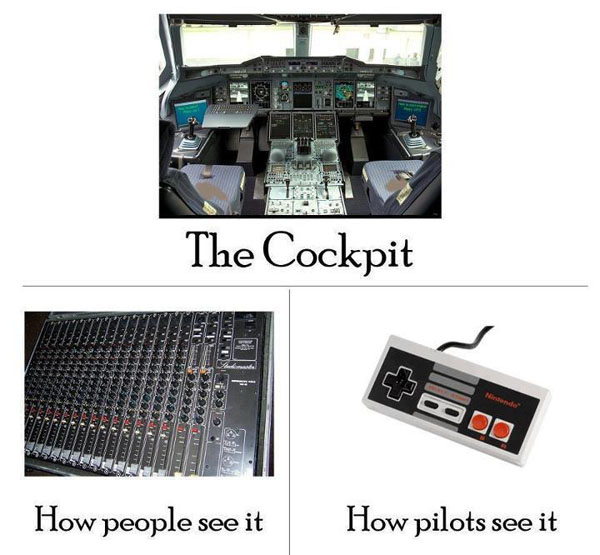
\includegraphics[width=\linewidth]{01.tablero.instrumentos/imagenes/1.1.introduccion/TheCockpit.jpg} \\
% {\tiny Fuente: \url{https://aviationhumor.net/flight-deck-cockpit-jokes-and-memes/}}

\Alerta{
    La habilidad de capturar y transmitir toda la informaci\'on que un piloto requiere, de forma segura y f\'acil de entender, ha sido un desaf\'io a trav\'es de la historia de la aviaci\'on, 
 \cite{FAA_Aviation_Maintenance_Technician_Handbook_Vol02}
}

En sus or\'igenes se equipaba a las aeronaves con pocos instrumentos debido a las cortas duraciones de los vuelos, sus costos y las complicaciones para el piloto en la interpretaci\'on de los mismos. \'este tipo de vuelo usualmente es conocido como \ac{VFR}.

% Hoy en d\'ia dicho concepto no est\'a vigente, entre otras razones por una mayor operatividad de las aeronaves, mayores tiempos de vuelo y la seguridad de sus tripulantes y pasajeros, por lo que este tipo de equipamiento se ha vuelto muy importante como as\'i tambi\'en sus costos. 

Los pilotos, cuya funci\'on es ser los ``\emph{cerebros}'' de la aeronave, deben tener conocimiento de todos los par\'ametros de la misma y los fen\'omenos que pueden ocurrir durante su operaci\'on, algunos de los cuales podr\'ian provocarle a sus sentidos indicaciones err\'oneas y, a veces, totalmente equivocadas. Es por ello que en el tiempo se han desarrollado todo tipo de instrumentos para asistir a los pilotos en sus funciones. 

La operaci\'on de una aeronave en condiciones atmosf\'ericas u horarias no comunes condujo a establecer las \ac{IFR}, para las cuales se necesita una capacitaci\'on y certificaci\'on adecuadas.

Las reglas de vuelo, tanto \ac{VFR} como \ac{IFR}  est\'an establecidas en Argentina por la \ac{ANAC} 
en la 
{RAAC 91} 
bajo el t\'itulo \emph{Reglas de vuelo por instrumentos (IFR)} 
y quien realiza un vuelo de \'este tipo debe poseer una 
\emph{Habilitación de Vuelo por Instrumentos} otorgada por la autoridad competente.

\begin{tcolorbox}
  La reglamentaci\'on de la ANAC se encuentra comprendida en las \ac{RAAC}, y pueden ser consultadas 
\href{http://www.anac.gov.ar/anac/web/index.php/2/120/normativa/raac-dnar}{en su sitio web}. 
En el mismo se encuentra la 
\href{http://www.anac.gov.ar/anac/web/uploads/normativa/raac/raac_vigentes/por_parte/parte-91-r-1-18.pdf}{RAAC Parte 91 ``{\it Reglas de vuelo y operación general }''}. 
A su vez tambi\'en  se dispone de la  
\href{http://www.anac.gov.ar/anac/web/uploads/normativa/raac/parte-91_subaprte1.pdf}{Subparte I - Aeronaves } 
y de la 
\href{http://www.anac.gov.ar/anac/web/uploads/normativa/raac/parte-91_subparte2.pdf}{Subparte II - Aviones grandes y turborreactores }.

\end{tcolorbox}

Es interesante observar la 
evoluci\'on en el tiempo de las cabinas de vuelo en donde se disponen los instrumentos de las aeronaves, ver Figura \ref {fig:01.evolucion.cabina}.


\begin{figure}[!htb]
  \centering
  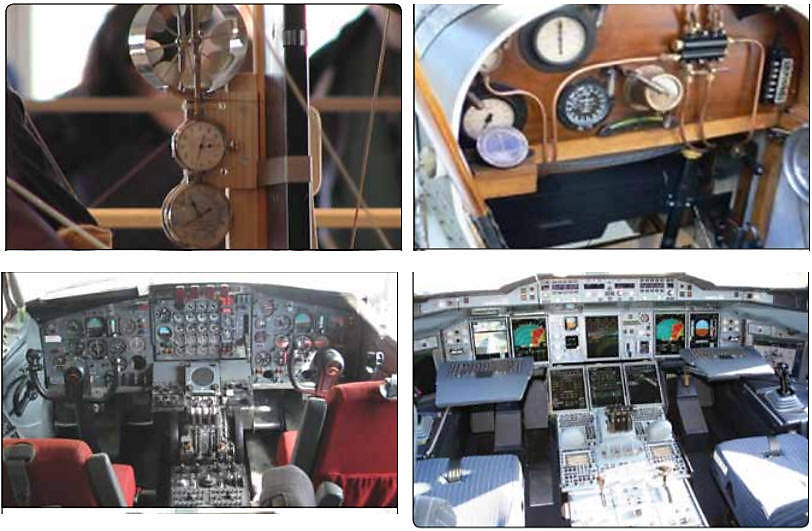
\includegraphics[height=0.6\linewidth, width=0.9\linewidth]{01.tablero.instrumentos/U01.imagenes/1.1.introduccion/evolucion_cabina.jpg} 

  \caption{{ Arriba izquierda: Wright Flyer, Arriba derecha: avi\'on primera guerra mundial, \\
      Abajo izquierda: Boeing 707 entre los '60 y '70, Abajo derecha: Airbus A380.}\\
    {\tiny Fuente:
      \url{https://www.waybuilder.net/free-ed/SkilledTrades/Aviation/AvAirframes/10AiInstrumt/10AiInstrumtFra.asp}}
  }
  \label{fig:01.evolucion.cabina}
\end{figure}

La evoluci\'on que ocurri\'o en el tiempo de los tableros de instrumentos de aeronaves puede apreciarse en la Figura \ref{fig:01.evolucion.tableros.instrumentos}

\begin{landscape}
  \begin{figure}[!htb]
    \centering
    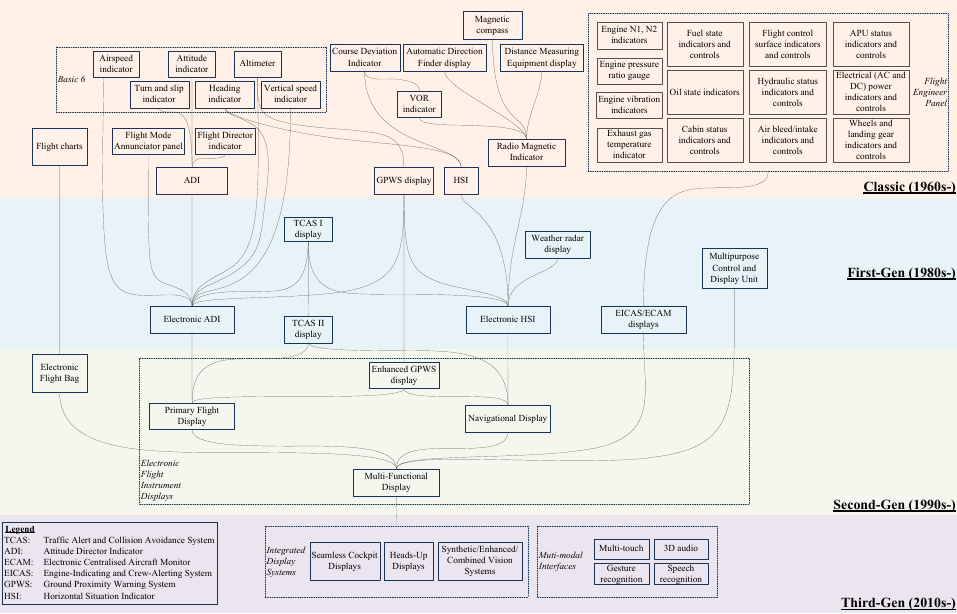
\includegraphics[width=\linewidth]{01.tablero.instrumentos/imagenes/1.1.introduccion/evolucion_cabina_00.png}

    \caption{Evoluci\'on de tableros de instrumentos en aeronaves
      \protect\cite{Lim2018AvionicsHI}.}
    \label{fig:01.evolucion.tableros.instrumentos}
  \end{figure}
\end{landscape}




\subsection{Ergonom\'ia}
\label{sec:ergonomia}

\begin{tcolorbox}
{\bf Ergonom\'ia:} 
\emph{Del griego.
  %	\griego{\'ergon}
  ''ergon'' (trabajo) y ``nom\'ia''
  % ( \griego{n\'omos}
  ``nomos'' (regla, ley),
  m\'as el sufijo ``ia'' (cualidad))}\\
1. f. Estudio de la adaptaci\'on de las m\'aquinas, muebles y utensilios a la persona que los emplea habitualmente, para lograr una mayor comodidad y eficacia.\\
2. f. Cualidad de ergon\'omico (adaptado a las condiciones del
usuario). \emph{El puesto de conducci\'on tiene buena ergonom\'ia.}

\begin{flushright}
  \textcolor{blue}{\it Fuente: Real Academia Espa\~nola }
\end{flushright}

\end{tcolorbox}

\emph{La Ergonom\'ia (o Factores Humanos) es la disciplina cient\'ifica relacionada con la comprensi\'on de las in\-te\-rac\-cio\-nes entre los seres humanos y los elementos de un sistema, y la profesi\'on que aplica teor\'ia, principios, datos y m\'etodos de dise\~no para optimizar el bienestar humano y todo el desempe\~no del sistema.
}
{\tiny Fuente: Asociaci\'on Internacional de Ergonom\'iía (IEA) \,
\url{https://www.iea.cc/whats/}}


\subsubsection{Ergonom\'ia Cognitiva}
\label{sec:01.ergonomia.cognitiva}

\begin{tcolorbox}
  ``{\it Se ocupa de los procesos mentales, tales como la
    percepci\'on, la memoria, el razonamiento y la respuesta motora,
    que afectan a las interacciones entre los seres humanos y otros
    elementos de un sistema. Los temas relevantes incluyen carga de
    trabajo mental, la toma de decisiones, el rendimiento experto, la
    interacci\'on persona-computadora, la fiabilidad humana, el
    estr\'es laboral y la forma como estos pueden estar relacionados
    con el dise\~no de los sistemas humanos. La ergonom\'ia cognitiva
    estudia los procesos de cognición en el trabajo y ajustes
    operativos, a fin de optimizar el bienestar humano y el
    rendimiento del sistema. } `` \cite{Asociacion_int_ergonomia}
\end{tcolorbox}

El campo de la Ergonom\'ia Cognitiva surgi\'o predominantemente al final de la d\'ecada de 1970 con la llegada de la computadora personal y los nuevos desarrollos en los campos de la psicolog\'ia cognitiva y la inteligencia artificial. Se contrasta con la tradici\'on de la ergonom\'ia f\'isica porque ``\emph{la ergonom\'ia cognitiva es... la aplicaci\'on de la psicolog\'ia cognitiva al trabajo... para lograr la optimizaci\'on (entre la gente y su trabajo) ... con respecto a al bienestar y productividad.}'' \cite{ergonomia_cognitiva_long_john}.

\begin{tcolorbox}
  Mayores detalles sobre Ergonom\'ia Cognitiva pueden consultarse en \cite{van_der_Veer} 
\end{tcolorbox}

Un esquema del modelo de procesamiento de informaci\'on puede observarse en la Figura \ref{fig:01.modelo.de.procesamiento.informacion.humano}.

\begin{figure}[!htb]
  \centering
  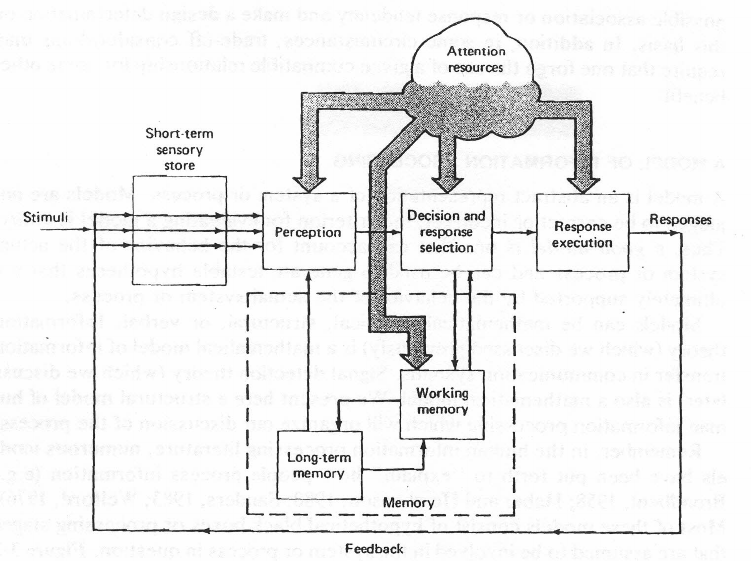
\includegraphics[width=0.8\linewidth]{01.tablero.instrumentos/U01.imagenes/1.1.introduccion/01-modelo_humano_procesamiento_informacion.png}
  
  \caption{Modelo  de procesamiento de informaci\'on humano \protect\cite{sanders1993human}}
\label{fig:01.modelo.de.procesamiento.informacion.humano}
\end{figure}

%{\tiny Fuente: Romosquera, \url{https://commons.wikimedia.org/wiki/File:Procesamiento_de_la_Informaci\%C3\%B3n.png}  }


\subsubsection{ Ergonom\'ia F\'isica}
\label{sec:ergonomia.fisica}

La Ergonom\'ia F\'isica se ocupa de las caracter\'isticas anat\'omicas, antropom\'etricas, fisiol\'ogicas y biomec\'anicas del usuario, en tanto que se relacionan con la actividad f\'isica.

Sus temas m\'as relevantes incluyen posturas de trabajo, sobreesfuerzo, manejo manual de materiales, movimientos repetitivos, Lesiones M\'usculo-Tendinosas (LMT) de origen laboral, dise\~no de puestos de trabajo, seguridad y salud ocupacional \cite{wiki_ergonomia_fisica}. 

En la Figura \ref{fig:01.dimensiones.estandard.cabina} puede apreciarse un estudio de la dimensiones interiores de una cabina y la ubicaci\'on de la persona dentro de la misma.


\begin{figure}[!htb]
  \centering
  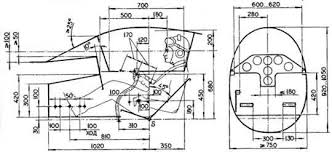
\includegraphics[width=0.9\textwidth]{01.tablero.instrumentos/U01.imagenes/1.1.introduccion/ergonomia_fisica.jpeg}
  
  \caption{Dimensiones estandar del interior de una cabina \protect\cite{cabina_ergonomia_fisica}}
\label{fig:01.dimensiones.estandard.cabina}
\end{figure}
%{\tiny Fuente: \url{https://www.ijsr.net/archive/v6i2/ART2017582.pdf}}




\subsubsection{Ergonom\'ia Visual}
\label{sec:01.ergonomia.visual}


La Ergonom\'ia Visual, como dominio dentro de la rama de ergonom\'ia, se centra en recomendaciones b\'asicas que deben cumplir aquellas personas que, en el desempe\~no de su actividad, emplean largas horas trabajando con pantallas y monitores. Estas recomendaciones incluyen aspectos como la separaci\'on entre el usuario y la pantalla, la necesidad de separar la vista del monitor repetidamente y centrarla en un punto lejano, o los beneficios de un parpadeo repetido que hidrate las capas corneales del ojo \cite{wiki_ergonomia_fisica}. 

\begin{center}
  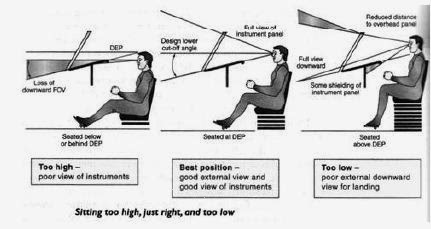
\includegraphics[width=0.7\textwidth]{01.tablero.instrumentos/U01.imagenes/1.1.introduccion/ergonomia_visual.jpg}
\end{center}
{\tiny Fuente: \url{http://avionics-system-design.blogspot.com/2013/12/ergonomics-of-aircraft-cockpit.html}}



\subsection{Formas de presentaci\'on de la informaci\'on}
\label{sec:formas.presentacion.informacion}

En vuelo, una aeronave y su tripulación forman un bucle de sistema ``{\it ser humano-máquina}'' que, según el tamaño y el tipo de la aeronave, puede ser bastante simple o muy complejo, ver Figura \ref{fig:01.bucle.ser.humano.maquina}. 
La función de la tripulaci\'on dentro de este bucle es la de controlador y el alcance de su función se rige por la simplicidad o no de la máquina como un todo integrado. 
Por ejemplo, al volar manualmente un avión e iniciar los ajustes a los sistemas esenciales se dice que la función del controlador es completamente activa. Si, por el contrario, el vuelo de un avión y los ajustes a los sistemas esenciales son automáticos, entonces la función del controlador pasa a ser de monitoreo, con la posibilidad de volver a la función activa en caso de falla de los sistemas.


\begin{figure}[!htb]
  \centering
  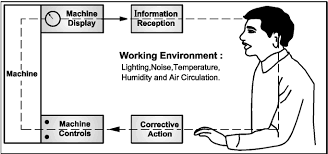
\includegraphics[width=0.5\textwidth]{01.tablero.instrumentos/U01.imagenes/1.1.introduccion/01-bucle_hbre_maquina.png}
  
  \caption{Bucle ser humano-m\'aquina \protect\cite{cabina_ergonomia_fisica}}
\label{fig:01.bucle.ser.humano.maquina}
\end{figure}



Los instrumentos tienen un rol vital en el circuito de control ya que son el medio de comunicar datos entre los sistemas y el controlador. Por lo tanto, para que un responsable del control  pueda obtener el máximo de calidad de control y, también para minimizar el esfuerzo mental en la interpretación de los datos, es necesario prestar la máxima atención al contenido y la forma de visualización de los datos.

Las formas más comunes de visualización de datos aplicadas a los instrumentos de aeronaves son:

\begin{enumerate}[a)]
\item \textbf{Cuantitativas}, en las que la cantidad variable que se mide
  se presenta en términos de un valor numérico y por la posición
  relativa de un puntero o índice, y
\item \textbf{Cualitativas}, en en el que la
  información se presenta en forma simbólica o pictórica.
\end{enumerate}

  \begin{itemize}
  \item {\bf Presentaciones cuantitativas:} ver Figura \ref{fig:01.presentaciones.cuantitativas}.
    \begin{itemize}
      \item Escala circular, es un m\'etodo cl\'asico de presentaci\'on de informaci\'on en forma cuantitativa. La escala del instrumento est\'a constitu\'ido por las correspondientes marcas de graduaci\'on. Su cantidad depende es una soluci\'on de compromiso seg\'un el tipo de informaci\'on a brindar: pocas marcas podr\'ian perder informaci\'on vital y producir errores de lectura, por el contrario una cantidad excesiva de marcas sobrecargar\'ia al operador y le insumir\'ia un tiempo excesivo de lectura. Los tama\~nos de las marcas son importantes y, usualmente, se numeran las marcas de cifras m\'as grandes las cuales presentan una longitud mayor. Es de suma importancia que el n\'umero de puntos posibles de medici\'on se elija cuidadosamente a fin de obtener lecturas r\'apidas y precisas.

El espaciado de las marcas 

      \begin{itemize}
         \item Escala lineal
         \item Escala no lineal (cuadr\'atica, logar\'itmica)
      \end{itemize}
       \item Escala longitudinal
       \item Presentaci\'on digital
    \end{itemize}
  \item {\bf Presentaciones cualitativas:} la información se presenta en forma simbólica o pictórica para mostrar la condición de un sistema como por ejemplo si el valor de una salida está aumentando o disminuyendo, el movimiento de un componente, etc. 

%En la Figura xx se muestran dos ejemplos típicos. El sincroscopio en (a) se utiliza junto con un rev./min. sistema indicador de una aeronave que tiene una disposición múltiple de motores de tipo hélice, y sus punteros, que simbolizan las hélices, solo giran para mostrar las diferencias de velocidad entre motores. La pantalla, que se muestra en (b), es un buen ejemplo de una que indica el movimiento de componentes; en este caso, superficies de control de vuelo, flaps de aterrizaje y deflectores de aire. El instrumento contiene diecisiete mecanismos eléctricos separados, que al ser accionados por transmisores, colocan elementos indicadores simbólicos de modo que aparezcan en varios ángulos detrás de las aberturas en el dial principal.



  \item {\bf Presentaciones directoras} ver Figura \ref{fig:01.presentaciones.directoras},  son aquellas que están asociadas principalmente con la actitud de vuelo y los datos de navegación.  Es importante presentarlos de una manera que indique al piloto qué movimientos de control debe hacer para corregir cualquier desviación de una trayectoria de vuelo deseada o para hacer que la aeronave realice una maniobra específica. 
En el desarrollo de este tipo de visualización debe existir una estrecha relación entre la dirección de los movimientos de control y el puntero del instrumento o elemento indicador de tipo simbólico, esto es los movimientos deben ser en el sentido "natural" para que el piloto pueda obedecer las ``\emph{directivas}'' o ``\emph{demandas}'' de la pantalla.
 
 \end{itemize}

  \begin{figure}[!htb]
    \centering
\subfigure[Escala circular cuantitativa \protect\cite{pallett1992aircraft}]{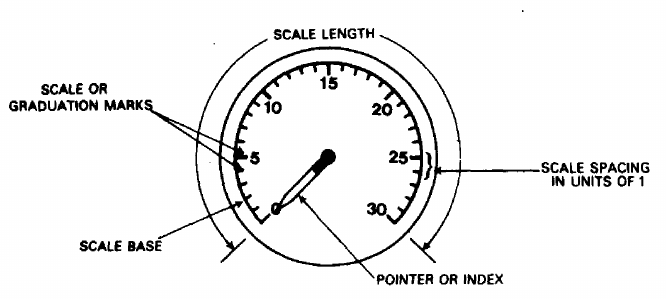
\includegraphics[width=0.45\textwidth]{01.tablero.instrumentos/U01.imagenes/1.2.clasificacion.instrumentos/escala_circular_cuantitativa.png}    }
\subfigure[a)Lineal, b) Ley cuadr\'atica , c) Ley logaritmica \protect\cite{pallett1992aircraft}]{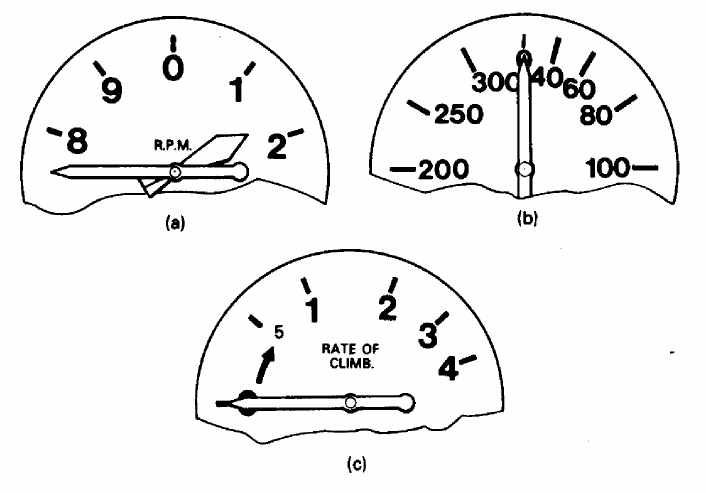
\includegraphics[width=0.45\textwidth]{01.tablero.instrumentos/U01.imagenes/1.2.clasificacion.instrumentos/escala_circular_lineal_no_lineal.png}}

\subfigure[a)Escalas conc\'entricas, (b) escalas fijas y giratorias, (c) escala com\'un tres agujas, (d) aguja dividida \protect\cite{pallett1992aircraft}]{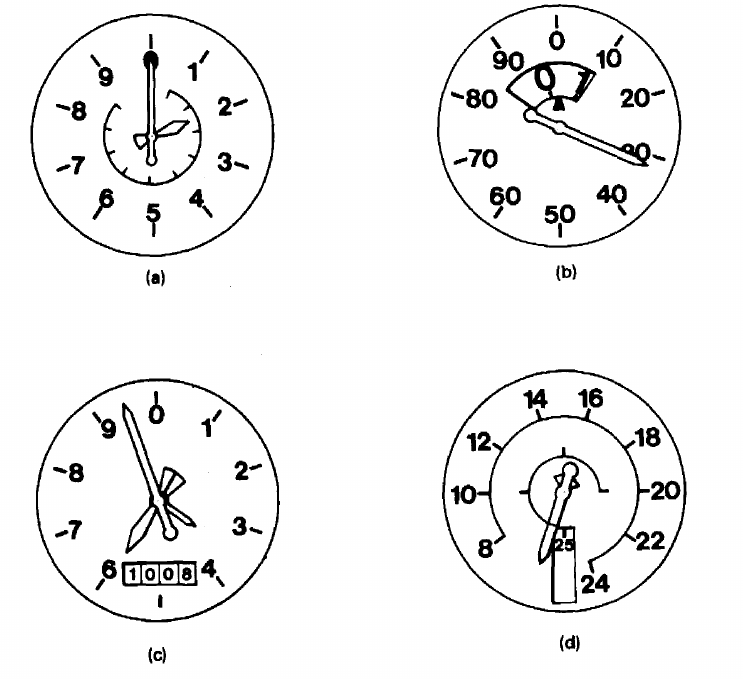
\includegraphics[width=0.45\textwidth]{01.tablero.instrumentos/U01.imagenes/1.2.clasificacion.instrumentos/escala_gran_alcance.png}}
\subfigure[Escala longitudinal \protect\cite{pallett1992aircraft}]{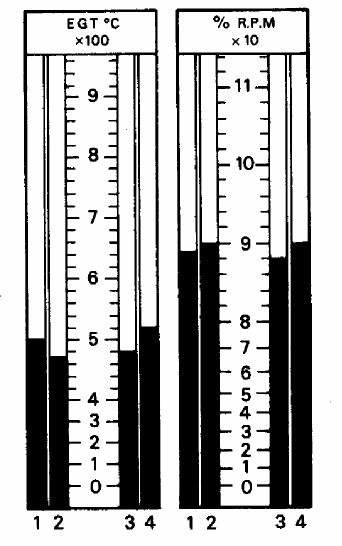
\includegraphics[width=0.35\textwidth]{01.tablero.instrumentos/U01.imagenes/1.2.clasificacion.instrumentos/longitudinal.png}}

    \caption{Presentaciones cuantitativas}
    \label{fig:01.presentaciones.cuantitativas}
  \end{figure}

  \begin{figure}[!htb]
    \centering
        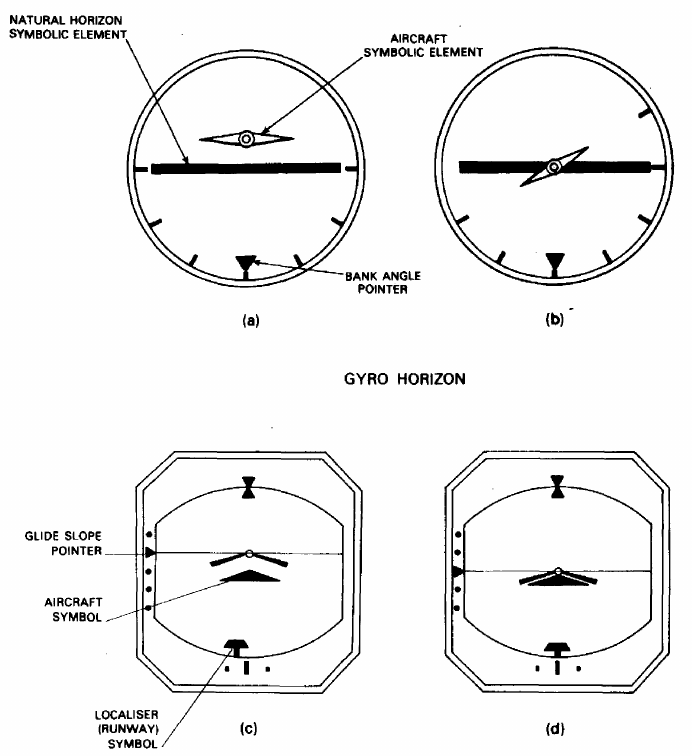
\includegraphics[width=0.75\textwidth]{01.tablero.instrumentos/U01.imagenes/1.2.clasificacion.instrumentos/director.png}
    \caption{Presentaciones directoras \protect\cite{pallett1992aircraft}}
    \label{fig:01.presentaciones.directoras}
  \end{figure}


%     \begin{tabular}{ccc}
%     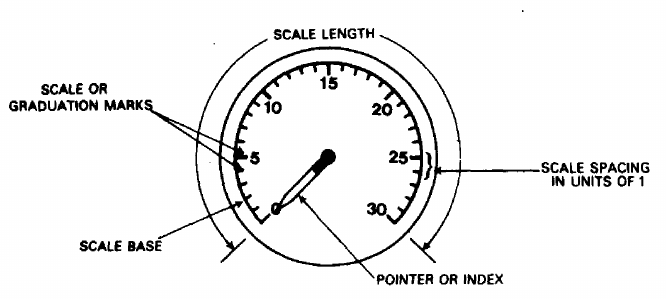
\includegraphics[width=0.45\textwidth]{01.tablero.instrumentos/U01.imagenes/1.2.clasificacion.instrumentos/escala_circular_cuantitativa.png} & \hspace{3mm}
% &     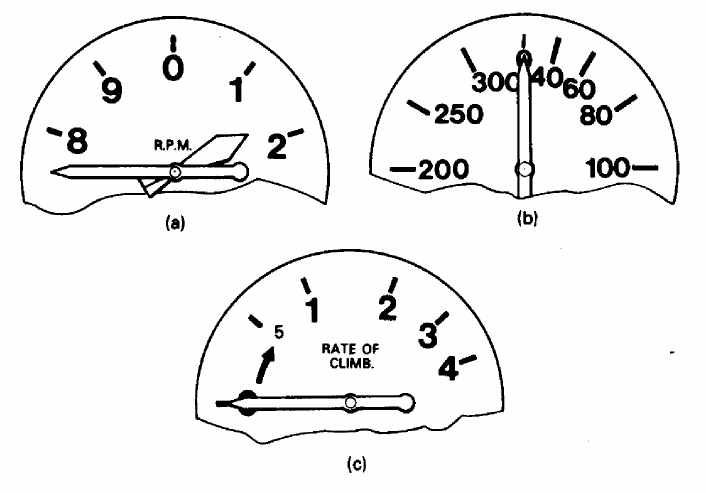
\includegraphics[width=0.45\textwidth]{01.tablero.instrumentos/U01.imagenes/1.2.clasificacion.instrumentos/escala_circular_lineal_no_lineal.png}
% \\
% 	Escala circular cuantitativa & 
% & \parbox{0.45\textwidth}{a) Lineal, b) ley cuadr\'atica, \\c) ley logaritmica}
% \\
%   \end{tabular}

% {\tiny Referencia: \cite{pallett1992aircraft}}

%   \begin{tabular}{ccc}
%     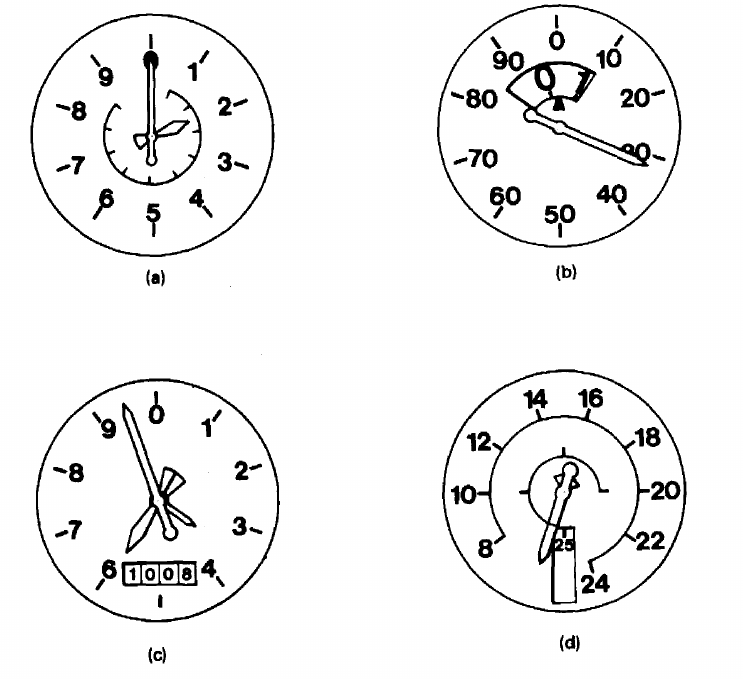
\includegraphics[width=0.45\textwidth]{01.tablero.instrumentos/U01.imagenes/1.2.clasificacion.instrumentos/escala_gran_alcance.png} & \hspace{3mm}
% &     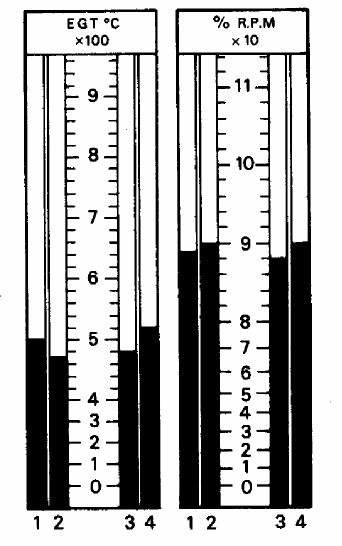
\includegraphics[width=0.35\textwidth]{01.tablero.instrumentos/U01.imagenes/1.2.clasificacion.instrumentos/longitudinal.png}
% \\
% \parbox{0.45\textwidth}{\small a)Escalas conc\'entricas, (b) escalas fijas y giratorias, (c) escala com\'un tres agujas, (d) aguja dividida}
% &
% & {\small Escala longitudinal}
% \\
%   \end{tabular}
% {\tiny Referencia: \cite{pallett1992aircraft}}


%   \begin{tabular}{ccc}
%     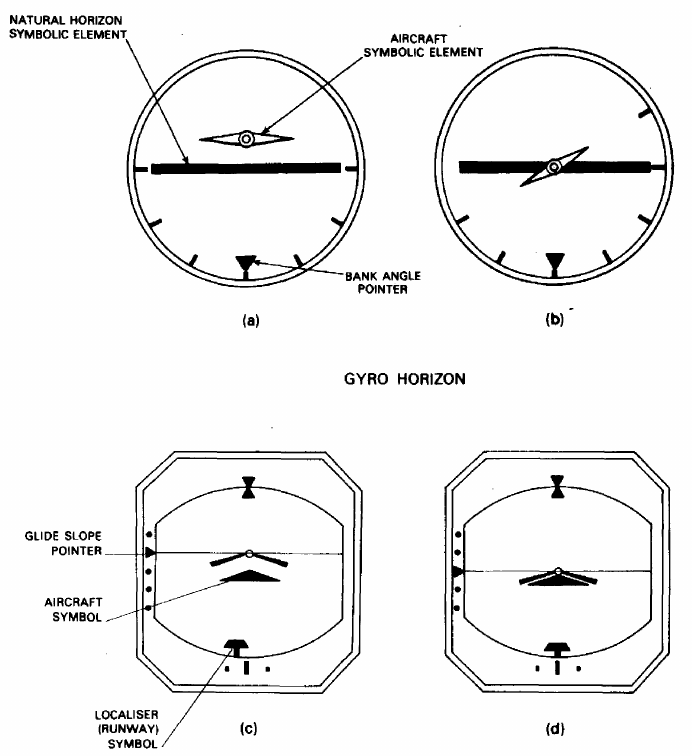
\includegraphics[width=0.45\textwidth]{01.tablero.instrumentos/U01.imagenes/1.2.clasificacion.instrumentos/director.png} & \hspace{3mm}
% &     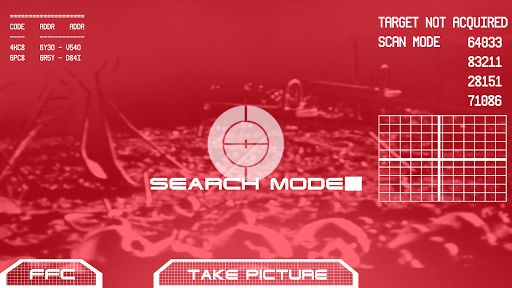
\includegraphics[width=0.5\textwidth]{01.tablero.instrumentos/U01.imagenes/1.2.clasificacion.instrumentos/terminator_hud.png}
% \\
% \parbox{0.45\textwidth}{Director de vuelo}
% &
% & Terminator Hud
% \\
%   \end{tabular}

% Head-Up Display
% Versión 2023
  
\subsubsection{Head Up Display }
\label{sec:HUD}
  
La simplicidad o no de presentaci\'on de la informaci\'on est\'a directamente involucrada a el número de instrumentos, por la cantidad de trabajo y secuencias de monitoreo de instrumentos que debe realizar un piloto durante las diversas fases del vuelo. En la fase crítica de aproximación y aterrizaje un piloto debe transferir su atención con mayor frecuencia de los instrumentos a las referencias fuera de la aeronave y viceversa. Un proceso de transición que lleva mucho tiempo y es fatigoso como resultado del constante reenfoque de los ojos.

Por lo tanto, se ha desarrollado un método para aliviar estos problemas en el que los datos de vuelo vitales se presentan al mismo nivel que la línea de visión del piloto cuando se ven referencias externas, es decir, cuando se mantiene una posición de ``{\it cabeza arriba}'' (head up). Los componentes de un sistema típico de visualización de esta forma, denominado \ac{HUD}, se pueden observar en la Figura \ref{fig:01.HUD} \cite{MikesFlightDeck}.

La cantidad de datos requeridos se rige por los requisitos de las diversas fases de vuelo y la función operativa de una aeronave, es decir, civil o militar, pero los  parámetros que se muestran son básicos. Los datos se transmiten desde una unidad de computadora de datos al tubo de rayos catódicos  cuya presentación es proyectada por el sistema óptico al infinito. La longitud, o rango, de las escalas está determinada por los requisitos operativos, pero normalmente solo cubren bandas estrechas de información de velocidad y altitud. Esto ayuda a reducir las marcas irrelevantes y el tiempo necesario para leer e interpretar. La  proyecci\'on óptica como una imagen simbólica compuesta sobre una placa reflectora transparente, o directamente sobre el parabrisas es lo que ve el piloto. %Se observará que la presentación de la actitud se asemeja a la de un horizonte giroscópico normal, y también que la velocidad y la altitud se presentan mediante marcadores que se registran contra escalas lineales horizontales y verticales. 

El HUD usa aplicaciones ópticas para agregar símbolos generados por computadora al campo de visión frontal del piloto, por esto se dice que es una clase de pantalla colimada, al parecer que las imágenes añadidas estan en el infinito óptico. Esto proporciona dos ventajas principales:

\begin{itemize}
\item Las imágenes permanecen alineadas con la vista exterior independientemente de cómo cambie el punto de vista del piloto.

\item El piloto no necesita volver a enfocar los ojos cuando cambia entre otro instrumento y la lectura de los datos del HUD. 
\end{itemize}

Esto significa que el sistema óptico es más complejo que un simple espejo parcialmente reflectante.

Una lente esférica, plano-convexa colimará una imagen, pero este enfoque tan simple tiene algunas deficiencias: introducirá distorsión geométrica en la imagen, no todos los colores estarán enfocados para la misma posición de la lente y cuando el centro de la imagen esté enfocado, los bordes de la imagen no lo estarán.

Se emplean lentes esféricos a pesar de estas limitaciones porque se pueden hacer formas esféricas con gran precisión con costos moderados. Las lentes asféricas fabricadas con una precisión similar pueden tener propiedades ópticas sustancialmente mejores, pero las complejidades de fabricación pueden hacer que el costo sea prohibitivo.

De todas maneras las lentes asféricas no son la respuesta final porque sólo pueden corregir distorsiones geométricas, puesto que las lentes, esféricas o no, funcionan refractando la luz y los ángulos de refracción cambian con la longitud de onda de ésta. Las lentes asféricas están sujetas a la aberración cromática al igual que las lentes esféricas.

El conjunto de óptica de colimación HUD consta de varias lentes simples. Al menos una de las lentes estará hecha de un material con un índice de refracción diferente. Las lentes individuales y los materiales de las lentes se eligen de modo que las aberraciones de las lentes individuales tiendan a cancelarse, dando como resultado una lente compuesta que tiene un rendimiento superior al de sus componentes.

Combinadores

Parcialmente reflectante

Los combinadores vienen en varias variedades. Uno simple es un espejo plano parcialmente plateado. Es viable pero pierde luz. Si tiene una relación de transmisión del 50\%, la mitad pasa y la otra mitad se refleja. Esto no es un problema para los datos de HUD, ya que la fuente de HUD se puede hacer más brillante. Sin embargo, es un problema con respecto a la visión delantera del piloto. La mitad de eso también se refleja. Puede jugar con la relación de transmisión para reducir la pérdida de visión hacia adelante, pero eso solo funciona hasta ahora.

Otra característica molesta de estos combinadores es la presencia de reflejos internos. La luz se reflejará en las superficies delantera y trasera. Los reflejos aparecen como imágenes fantasma.

Los reflejos internos se pueden minimizar utilizando un revestimiento antirreflectante en la superficie no reflectante del sustrato del espejo. El recubrimiento genera reflejos en sus superficies frontal y posterior. El grosor del recubrimiento se controla de modo que la reflexión de la superficie posterior esté desfasada con la reflexión de la superficie frontal. Al estar fuera de fase, se anulan entre sí. El índice de refracción se elige de manera que las dos reflexiones sean de la misma magnitud para asegurar la mejor cancelación. Los revestimientos antirreflectantes se ajustan a una sola longitud de onda de luz, pero dan resultados adecuados en una gama de colores.

Dicroico

Un combinador mejorado hace uso de un espejo dicroico. Esto es similar a un recubrimiento antirreflectante, pero se utilizan muchas capas y el grosor del recubrimiento se elige para mejorar el reflejo de una longitud de onda particular. Otras longitudes de onda pasan con atenuación mínima. Cuando se usa un espejo dicroico, una banda estrecha de colores se bloquea fuera de la vista frontal del piloto y se reemplaza por los datos del HUD. Debido a que el color de la pantalla HUD coincide con la característica dicroica, prácticamente toda la luz generada por HUD se dirige al piloto y solo se bloquea una pequeña cantidad de luz exterior. Un combinador dicroico también está sujeto a reflexiones internas. Se utiliza un revestimiento antirreflectante en la parte trasera del combinador para controlar esto.

Catadióptrico

El combinador no tiene que ser plano. Se puede usar un combinador curvo para implementar parte de toda la colimación. Esto generalmente se conoce como HUD catadióptrico. Catadióptrico se refiere a un sistema óptico que incorpora elementos reflectantes y refractivos. Una gran ventaja de las ópticas reflectantes es que no sufren aberración cromática. Al igual que las lentes, se fabrican más fácilmente en formas esféricas y, por lo tanto, también sufren de aberración esférica. Esto se puede corregir a través del diseño del sistema óptico tal como se corrige un sistema basado en lentes.

Holográfico

El término ``{\em HUD holográfico}'' puede recordar a una película de SciFi pero, lLa realidad es mucho simple. Un HUD holográfico simplemente usa un elemento óptico holográfico o HOE como combinador. Esta es una rejilla de difracción especializada que puede combinar y colimar. Los HOE pueden tener una longitud de onda muy específica para permitir que la cantidad máxima de luz del campo de visión delantero pase al piloto. Un HUD holográfico puede ofrecer un campo de visión más amplio para un peso dado que un HUD basado únicamente en lentes y/o espejos.


\begin{figure}[!htb]
  \centering
  \subfigure[Principio de funcionamiento del
  HUD ]{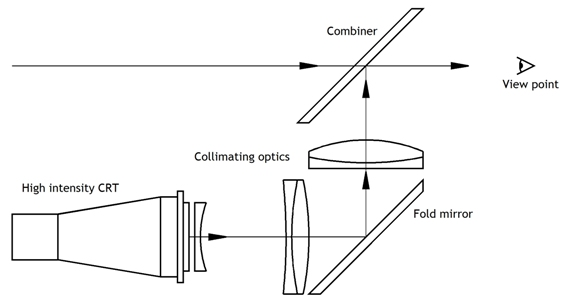
\includegraphics[width=0.45\textwidth]{01.tablero.instrumentos/U01.imagenes/1.2.clasificacion.instrumentos/hud_esquema.jpg}}
  \subfigure[Vista de un
  HUD]{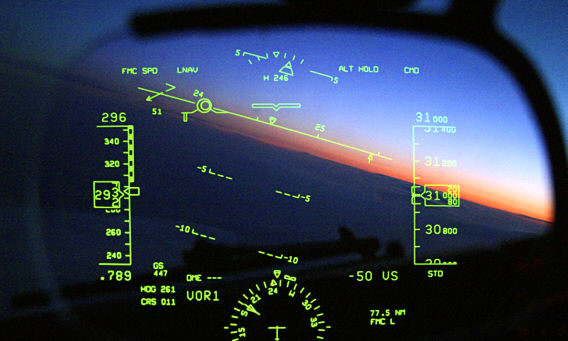
\includegraphics[width=0.45\textwidth]{01.tablero.instrumentos/U01.imagenes/1.2.clasificacion.instrumentos/hud.jpg}}
  
  \caption{HUD}
\label{fig:01.HUD}
\end{figure}


\begin{tcolorbox}
Un video interesante que cuenta la historia del HUD se encuentra en el siguiente link: 

  {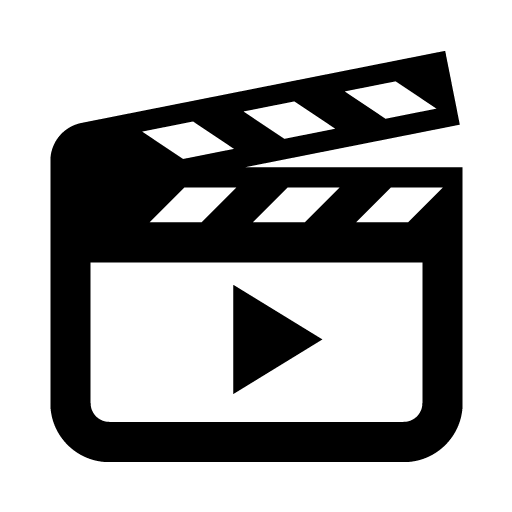
\includegraphics[width=0.1\textwidth]{01.tablero.instrumentos/U01.imagenes/Video.png}}\,
\href{https://www.youtube.com/watch?v=ypIbmfm7n8A}{The Evolution of the Head-Up Display}.
\vspace{3mm}


  Existen en el mercado peque\~nos \ac{HUD} para uso en aviaci\'on general como el provisto por la empresa Thales, el 
\href{https://www.thalesgroup.com/en/markets/aerospace/flight-deck-avionics-equipment-functions/topmax-wearable-hud-commercial-aircraft}{TopMax}.
\end{tcolorbox}


Tambi\'en se han desarrollado los \ac{EFVS} que son sistemas de visi\'on sint\'eticos, ver Figura \ref{fig:01.efvs}, 
 que proporciona una imagen de la escena y la muestra al piloto con el fin de proporcionar una imagen en la que la escena y los objetos en ella se pueden detectar mejor, esto es, un EFVS es un sistema que proporciona al piloto una imagen mejor que la visión humana sin ayuda. 

Los EFVS incluyen sensores de imágenes como una cámara a color, una cámara de infrarrojos o un radar y, normalmente una pantalla para el piloto, que puede ser una pantalla montada en la cabeza del mismo o una pantalla frontal. Un EFVS se puede combinar con un sistema de visión sintético para crear un sistema de visión combinado.
\href{https://www.youtube.com/watch?v=phbZintCgVA}{Video de un HUD/EFVS}.

\begin{figure}[!htb]
  \centering
\subfigure[EFVS]{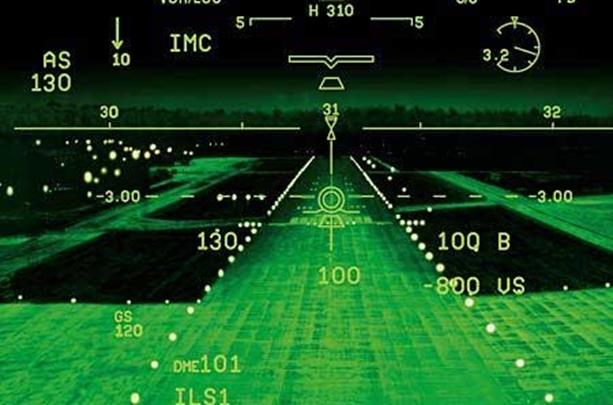
\includegraphics[width=0.45\textwidth]{01.tablero.instrumentos/U01.imagenes/1.2.clasificacion.instrumentos/EFVS_Photo.jpg}}
\subfigure[EFVS]{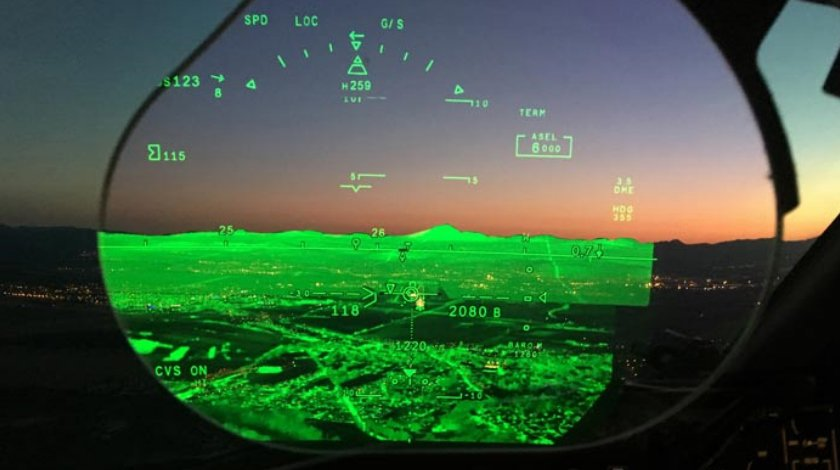
\includegraphics[width=0.45\textwidth]{01.tablero.instrumentos/U01.imagenes/1.2.clasificacion.instrumentos/efvs.jpg}}
  
  \caption{EFVS}
\label{fig:01.efvs}
\end{figure}







\section{Clasificaci\'on de los Instrumentos}
\label{sec:01.02.clasificacion.instrumentos}

Dentro de las distintas formas entre las cuales se podr\'ian clasificar los instrumentos de abordo, esto es por principio de funcionamiento, lectura directa, derivadores, integradores, a distancia, etc.; por lo anterior se puede clasificarlos seg\'un las magnitudes que miden. Seg\'un este criterio se los puede clasificar como:

\begin{itemize}
\item {\bf De Navegaci\'on:} que permiten determinar la posici\'on y el movimiento relativo de la aeronave con respecto a la Tierra.
\item {\bf De Actitud:} para conocer los \'angulos relativos que los ejes de la aeronave que pasan por su baricentro forman con la Tierra.
\item {\bf De Control:} entre los que se cuentan respecto al equipo propulsor y otros de equipos y sistemas varios de la aeronave.
\item {\bf Equipos Especiales:} tales como avisos de alarma, sistemas de seguridad, etc. 
\item {\bf Controles Autom\'aticos:} que reemplazan a los pilotos manteniendo cierta condici\'on de vuelo programada.
\end{itemize}

En la Figura \ref{fig:01.instrumentos.en.una.aeronave} tambi\'en puede observarse una clasificaci\'on de los instrumentos en una aeronave.

\begin{figure}[!htb]
  \centering
  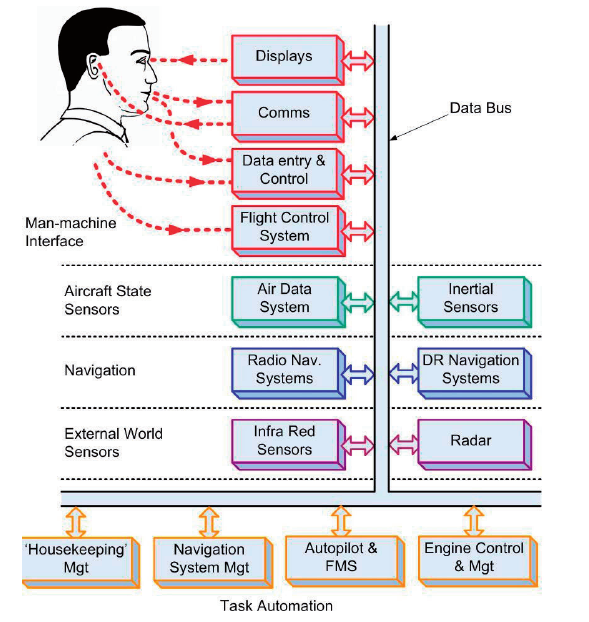
\includegraphics[width=0.9\textwidth]{01.tablero.instrumentos/U01.imagenes/1.2.clasificacion.instrumentos/tipos_instrumentos.png}  
  \caption{Instrumentos en una aeronave \protect\cite{Introduction_to_Avionics_Systems}}
  \label{fig:01.instrumentos.en.una.aeronave}
\end{figure}

%   Tambi\'en puede clasificarlos como se indica en la Tabla \ref{tab:01.clasificacion.instrumentos}.

% \begin{landscape}


% \begin{table}[!htb]
%   \centering
%   \caption{Clasificaci\'on de instrumentos}
%   \label{tab:01.clasificacion.instrumentos}

%   \begin{tabular}{cll} \hline \rowcolor{bubbles}
%     {\bf Tipo} & {\bf Instrumentos} & {\bf Descripci\'on / Requerimientos} \\ \hline

%    \parbox{0.15\textwidth}{\bf Sistema de \\ Pitot-Est\'atica}
%    &\parbox{0.30\textwidth}{
%         \begin{itemize}
%         \item Alt\'imetro
%         \item Veloc\'imetro
%         \item Indicador de Velocidad Vertical
%         \end{itemize}
%       }
%       &\parbox{0.65\textwidth}{ \scriptsize
%         \begin{itemize}
%         \item El sistema será hermético, excepto por los respiraderos a la atmósfera, y estará dispuesto de manera que la precisión de los instrumentos no se vea seriamente afectada por la velocidad, actitud o configuración de la aeronave; por humedad u otra materia extraña.

%         \item  El sistema debe estar provisto de una sonda de presión Pitot con calentamiento para evitar el mal funcionamiento debido a la formación de hielo.

%         \item Instalaci\'on de trampas de humedad para asegurar un drenaje positivo en todo el sistema.

%         \item  En aeronaves en las que se instalará un sistema alternativo o de emergencia, el sistema debe ser tan confiable como el primario y cualquier válvula selectora debe estar claramente marcada para indicar qué sistema está en uso.

%         \item  Las tuberías deben tener un diámetro interno tal que la diferenciade presión y la posibilidad de obstrucción por humedad se mantengan en un mínimo aceptable.

%         \item Cuando se utilicen ventilaciones estáticas, para evitar errores de guiñada, deberán estar situadas en lados opuestos de la aeronave y conectadas como un solo sistema. Cuando se prescriban sistemas duplicados, se proporcionará un segundo sistema similar.

%         \end{itemize}
%       } \\ \hline

%    \parbox{0.15\textwidth}{\bf Instrumentos giroscópicos}
%  	&
% 	&\parbox{0.65\textwidth}{ \scriptsize
% Los instrumentos giroscópicos pueden ser del tipo operado por vacío o eléctricamente, pero en todos los casos los instrumentos deben estar provistos de dos fuentes de energía independientes, un medio para seleccionar cualquiera de las fuentes de energía y un medio para indicar que la fuente de alimentación está funcionando satisfactoriamente. .

% La instalación y el sistema de suministro de energía deben ser tales que la falla de un instrumento, o del suministro de una fuente, o una falla en cualquier parte del sistema de suministro, no interfiera con el suministro adecuado de energía de la otra fuente.
% } \\ \hline
%     \end{tabular}
%   \end{table}


% \end{landscape}



%   \begin{tabular}{ccc}
%     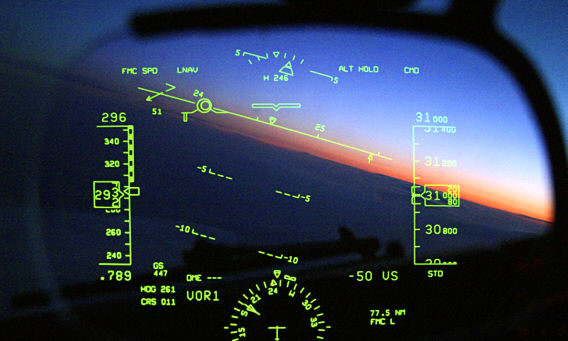
\includegraphics[width=0.45\textwidth]{01.tablero.instrumentos/U01.imagenes/1.2.clasificacion.instrumentos/hud.jpg} & \hspace{3mm}
% &     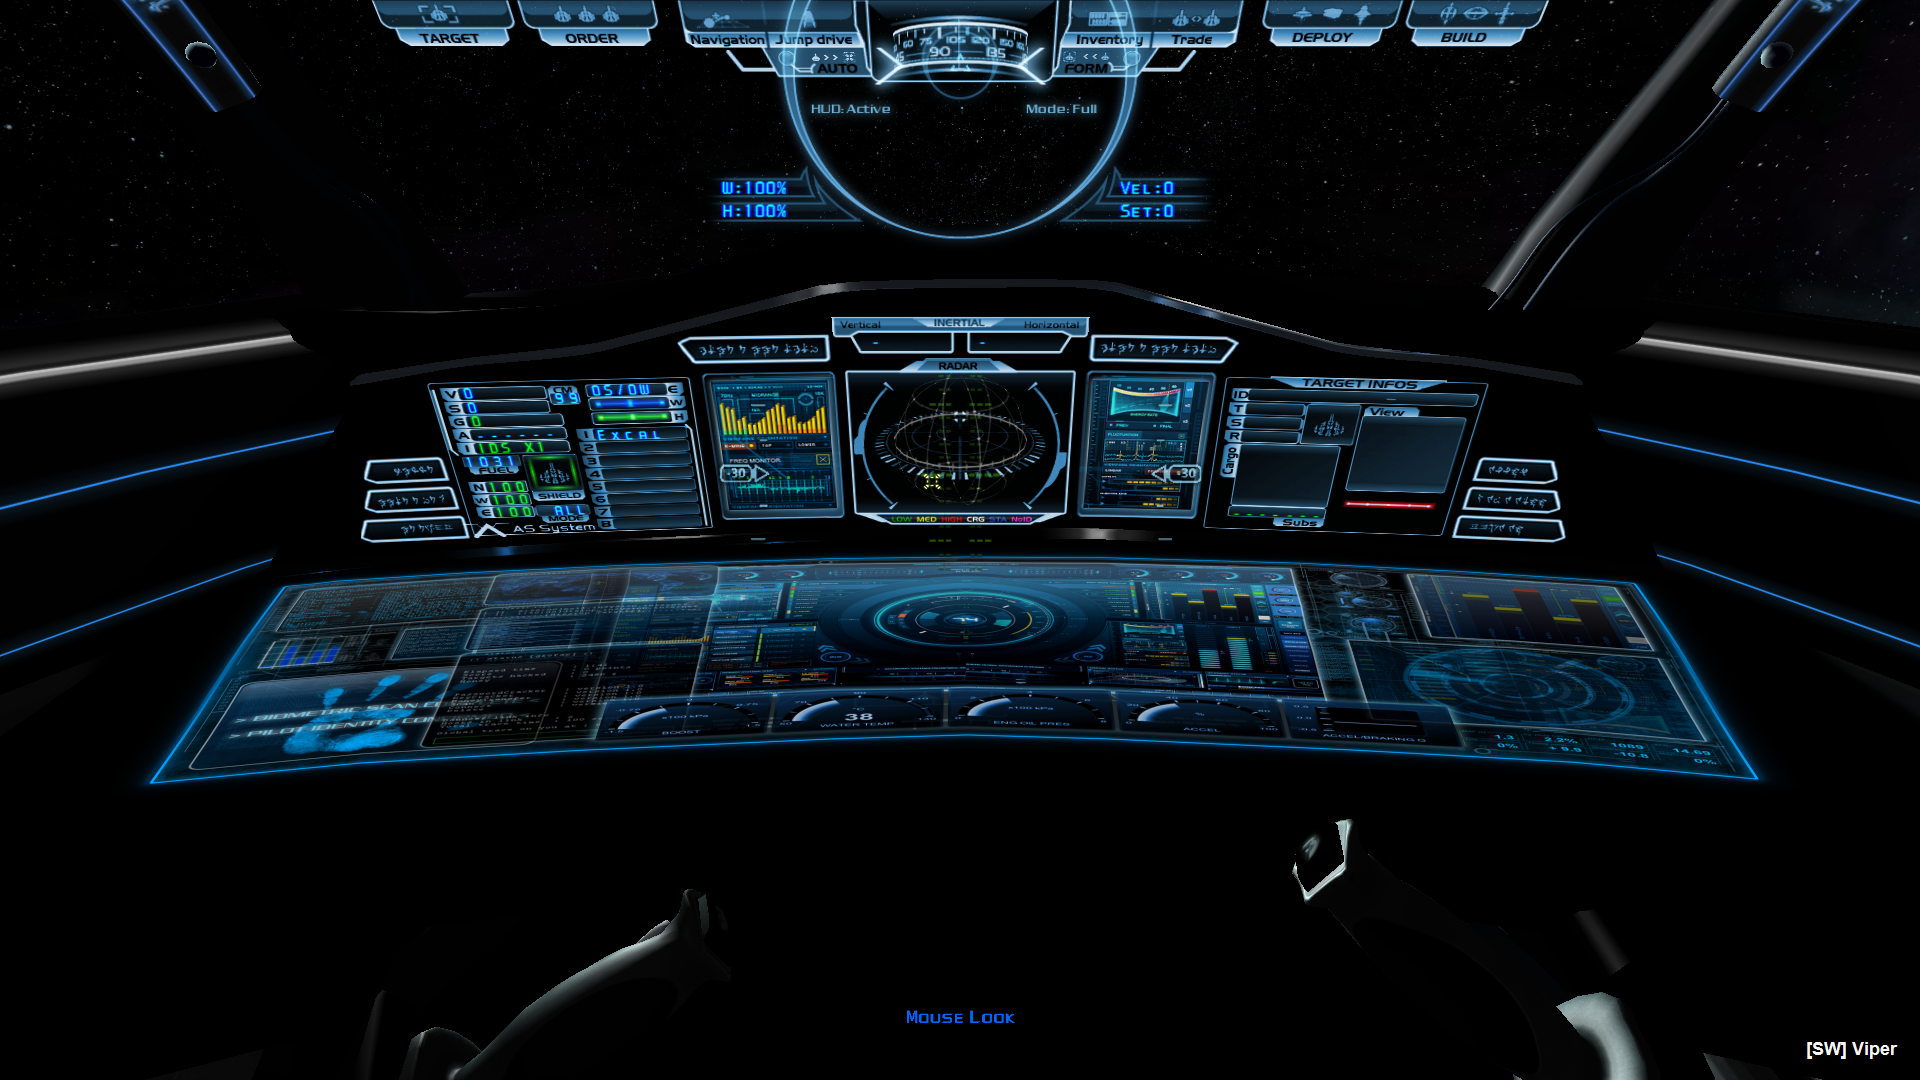
\includegraphics[width=0.5\textwidth]{01.tablero.instrumentos/U01.imagenes/1.2.clasificacion.instrumentos/viper_11.png}
% \\
% \parbox{0.45\textwidth}{Head Up Display}
% &
% & Hud futuro
% \\
%   \end{tabular}

  
% {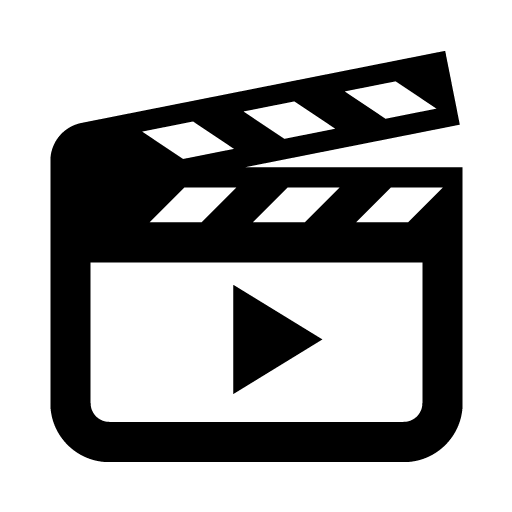
\includegraphics[width=0.1\textwidth]{01.tablero.instrumentos/U01.imagenes/Video.png}}\,
% Enhanced Flight Vision System \url{https://www.youtube.com/watch?v=DR9lyAM2YNE}
  


\section{Distribuci\'on Normalizada del Instrumental en el Tablero}
\label{sec:U01.03.distribucion.normalizada.instrumental}


En Argentina los requerimientos de instrumentos y equipos para aeronaves  civiles  motorizadas  con  Certificado de Aeronavegabilidad Estándar se encuentran contenidos en la \href{}{RAAC 91.205}, mencionada anteriormente.
En la misma se hace la distinci\'on entre:

\begin{itemize}
    \item Reglas de vuelo visual (VFR) diurno
    \item Reglas  de  vuelo  visual  (VFR)  nocturno
    \item Reglas de vuelo por instrumentos (IFR)
    \item Reglas de vuelo visual dentro del espacio aéreo controlado (VFR controlado)
\end{itemize}

En la Tabla \ref{tab:01.requerimientos.instrumentos.RAAC.91} se detallan los requerimientos anteriores.

% las CFAR se pueden encontrar en https://rgl.faa.gov/Regulatory_and_Guidance_Library/rgFAR.nsf/MainFrame?OpenFrameSet

A su vez se tienen las RAAC 23 y 25:

\begin{description}
\item[\href{https://www.anac.gov.ar/anac/web/uploads/upcg/raac/raac-23.pdf}{RAAC 23}] Estándares de aeronavegabilidad: aviones de categoría normal, utilitaria, acrobática y commuter.
\item[\href{https://www.anac.gov.ar/anac/web/uploads/upcg/raac/raac-25.pdf}{RAAC 25}]  Estándares de aeronavegabilidad: aviones de categoría transporte
\end{description}

En donde se hace mención de las 14 \ac{CFR} Part 23 y 25:

\begin{description}
\item[\href{https://www.law.cornell.edu/cfr/text/14/part-23/subpart-F}{14 \ac{CFR} Part 23 Sub Part F}]
\item[\href{https://www.law.cornell.edu/cfr/text/14/part-25/subpart-F}{14 \ac{CFR} Part 25 Sub Part F}] 
\end{description}

\newpage

  \begin{longtable}{m{0.25\textwidth}m{0.75\textwidth}}
    \caption{Requerimientos de instrumental seg\'un RAAC 91}
    \label{tab:01.requerimientos.instrumentos.RAAC.91} \\  \hline \rowcolor{bubbles}

      {\bf Reglas} & {\bf Instrumental requerido} \\ \hline \endfirsthead  \hline \rowcolor{bubbles}
      {\bf Reglas} & {\bf Instrumental requerido} \\ \hline \endhead

	\hline \endfoot  \hline \endlastfoot


      {\bf Reglas de vuelo visual (VFR) diurno}
      &
      {\scriptsize
        \begin{enumerate}
        \item Indicador de velocidad del aire.
        \item Un Baroaltímetro.
        \item Un reloj de precisión que indique las horas, minutos y
          segundos y que pueda mantener una exactitud de más o menos
          30 segundos durante un período de 24 horas.
        \item Indicador magnético de dirección.
        \item Tacómetro para cada motor.
        \item Medidor de presión (manómetro) de aceite, para cada
          motor que utilice circuito de presión de aceite.
        \item Medidor de temperatura (termómetro) para cada motor
          refrigerado por líquido.
        \item Medidor de temperatura de aceite para cada motor
          refrigerado por aire.
        \item Medidor de presión de admisión (Manifold) para cada
          motor alternativo capaz de mantener la potencia nominal de
          despegue desde el nivel del mar hasta una altitud
          establecida (tales como los motores con hélices de paso
          variable).
        \end{enumerate}
      } \\ \rowcolor{cyan!20}
\textbf{Reglas  de  vuelo  visual  (VFR)  nocturno}
& {\scriptsize
\begin{itemize}
	\item Todos los requeridos para VFR diurno
        \item Un indicador giroscópico de virajes.
\end{itemize}
}
\\ % \rowcolor{cyan!20}
\parbox{\linewidth}{\bf Reglas de vuelo por \\ instrumentos (IFR)}
& {\scriptsize
  \begin{itemize}
  \item Todos los requeridos para VFR diurno y nocturno
  \item Un sistema de radio comunicación que permita mantener una comunicación en ambos sentidos con las estaciones aeronáuticas en las frecuencias que prescriba la autoridad aeronáutica competente y el equipa-miento apropiado de navegación para las estaciones de tierra a ser utilizadas (VHF o HF). En caso de que no se disponga de equipo HF, las operaciones estarán sujetas a limitaciones especificadas en la RAAC 91.205.d.2.
  \item Un cronógrafo.
  \item Indicador giroscópico de velocidad de giro, excepto en las siguientes aeronaves:
    \begin{itemize}
    \item (i) Aviones con un tercer instrumento indicador de actitud
      que pueda medir todas las actitudes de vuelo a través de 360º de
      cabeceo y rolido y esté instalado de acuerdo con la Sección
      121.305 (j) de la Parte 121; y
    \item Helicópteros con un tercer
      instrumento indicador de actitud que pueda medir actitudes de
      vuelo entre +80º de cabeceo y +120º de rolido, esté instalado
      de acuerdo con la Sección 29.1303 (g) de la DNAR Parte 29.
    \end{itemize}
  \item Un Baroaltímetro sensitivo.
  \item Un Indicador de viraje y de inclinación lateral.
  \item Indicador giroscópico de inclinación lateral y cabeceo. (Horizonte artificial)
  \item Indicador giroscópico de dirección (girodireccional o equivalente).

{\it NOTA:Los  requerimientos  de:  indicador  de  viraje  y  de  inclinación  lateral,  indicador  de  actitud  de  vuelo  (horizonte  artificial),  e  indicador  de  rumbo  (giróscopo  direccional),  podrían  satisfacerse  mediante  combinaciones de instrumentos o sistemas integrados de dispositivos directores de vuelo, siempre que se conserven las garantías de que no ocurra una falla total, inherente a los tres instrumentos por separado.}

\item Medios para comprobar si es adecuada la fuente de energía que suministra energía a los instrumentos giroscópicos.
\item Un equipamiento aprobado de medición de distancia, \ac{DME}.
\item Un dispositivo que indique, en el compartimiento de la tripulación de vuelo, la temperatura exterior.
\item Un sistema indicador de la velocidad relativa con dispositivos que impidan su mal funcionamiento debido a condensación o a formación de hielo.
\item Un equipo \ac{VOR}.
\item Un equipo \ac{ADF} o equipo \ac{GNSS}.
\item Para los vuelos en que se proyecte aterrizar en condiciones meteorológicas de vuelo por instrumentos (IMC), el avión dispondrá de equipo que permita recibir las señales que sirvan de guía hasta un punto desde el cual pueda efectuarse un aterrizaje visual, \ac{ILS}.  

  \end{itemize}
}
\\  \rowcolor{cyan!20}
\parbox{\linewidth}{\bf Reglas de vuelo visual \\dentro del espacio aéreo\\ controlado\\ (VFR controlado)}
& {\scriptsize 
 Para vuelos VFR controlados dentro del espacio aéreo controlado, se requieren los siguientes equipamientos e instrumentos:
 \begin{itemize}
 \item Seg\'un las condiciones:
   \begin{itemize}
   \item Si el vuelo controlado es VFR – diurno, instrumentos y
     equipamientos especificados en Reglas de vuelo visual (VFR)
     diurno.
   \item Si el vuelo controlado es VFR – nocturno, instrumentos y
     equipamientos especificados en Reglas de vuelo visual (VFR)
     nocturno.
   \end{itemize}
 \item Un equipo VOR.
 \item Un equipo DME.
 \item Un variómetro.
 \item Un equipo ADF o equipo GNSS.
 \item Un  sistema  de  radiocomunicación  que  permita  mantener  una  comunicación  en  ambos  sentidos,  en  cualquier momento durante el vuelo con aquellas estaciones aeronáuticas en las frecuencias que prescriba la autoridad aeronáutica  competente  y  el  equipamiento  apropiado  de  navegación  para  las  estaciones  de  tierra  a  ser  utilizadas  (VHF  o HF).En  caso  de  que  no  se  disponga  de  equipo  HF,  las  operaciones  estarán  sujetas a las  limitaciones indicadas en RAAC 91.205.e.6.
 \item Un dispositivo que indique, en el compartimiento de la tripulación de vuelo, la temperatura exterior.
 \end{itemize}


}
\\

  \end{longtable}

%In 1937, the Royal Air Force selected six critical instruments to be installed in nearly all of its aircraft. Adopted by both commercial and general aviation aircraft manufacturers for decades thereafter, the arrangement became known as the “six pack.”

En 1937 la \ac{RAF} seleccion\'o seis instrumentos considerados esenciales en la cabina, conocidos como los ``\emph{basic six}'' (los seis b\'asicos), fue una distribuci\'on de instrumentos caracter\'istica de instrumentos en aviones brit\'anicos por los siguientes veinte a\~nos \cite{RAF_37}. Esta disposici\'on fu\'e adoptada tanto para aviaci\'on comercial como general por los fabricantes de aeronaves y es popularmente conocida como ``\emph{six pack}'''.
 
Esta distribuci\'on est\'a dividida en dos categor\'ias seg\'un se encuentren conectados al sistema de Pitot-Est\'atica o sean  Instrumentos Girosc\'opicos, en la Tabla \ref{tab:01.6-pack} puede observarse dicha clasificaci\'on y en la Figura \ref{fig:01-6-pack} su ubicaci\'on en el tablero de instrumentos.

\begin{figure}[!htb]
  \centering
  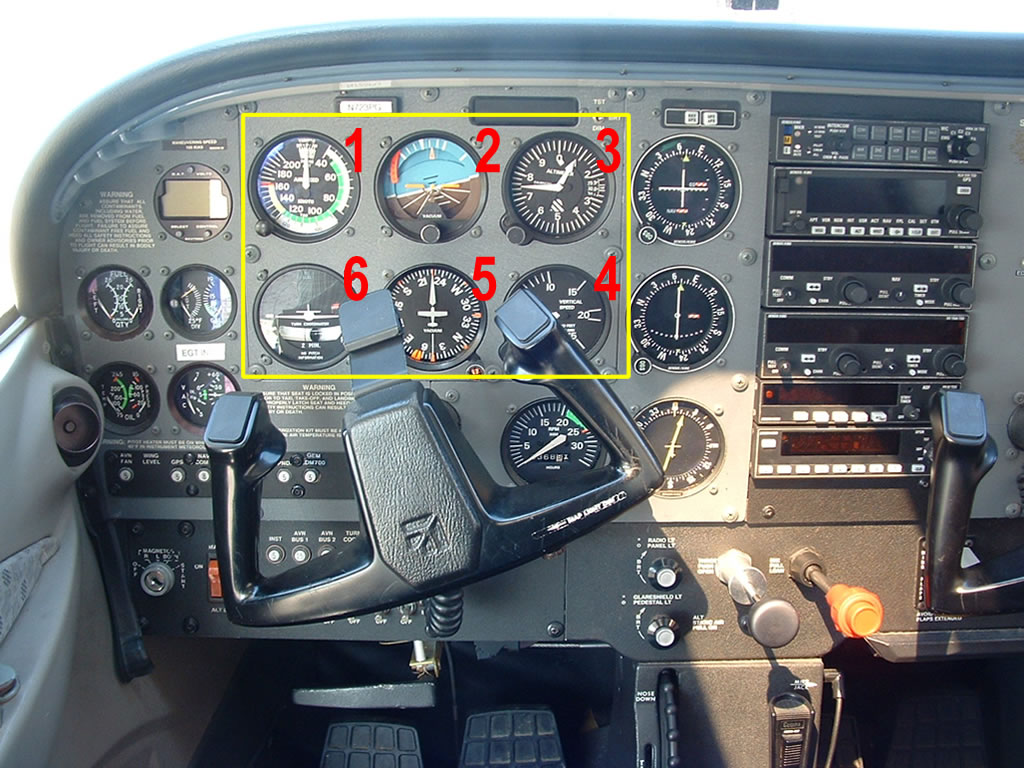
\includegraphics[width=0.8\linewidth]{01.tablero.instrumentos/imagenes/1.3.distribucion.normalizada.instrumental.en.tablero/01-Cessna-172-Instrument-Panel.jpg}
  \caption{Distribuci\'on de los basic six, \protect\cite{6-pack}}
  \label{fig:01-6-pack}
\end{figure}


\begin{table}[!htb]
  \centering
  \caption{Detalle de los instrumentos basic six}
  \label{tab:01.6-pack}
{\footnotesize
  \begin{tabular}{cm{0.35\textwidth}cc} \hline \rowcolor{azure} 
   \textcolor{white}{\bf Nro} & \centering \textcolor{white}{\bf Instrumento} 
	& \parbox{0.25\textwidth}{\textcolor{white}{\bf Instrumentos conectados \\al sistema de Pitot-Est\'atica}}
	& \parbox{0.15\textwidth}{\textcolor{white}{\bf Instrumentos girosc\'opicos}} \\ 
    {\bf 1} & Veloc\'imetro, \ac{ASI} & X & \\ \rowcolor{bubbles}
    {\bf 2 } & Indicador de Actitud, \ac{AI}, tambi\'en conocido como Horizonte Artificial & & X \\
{\bf 3} & Alt\'imetro & X & \\ \rowcolor{bubbles}
{\bf 4} & Indicador de Velocidad Vertical, \ac{VSI} & X & \\
{\bf 5} & Indicador de Rumbo, \ac{HI} & & X \\  \rowcolor{bubbles}
{\bf 6} & Indicador de Giro y Viraje, \ac{TC} & & X \\ \hline
  \end{tabular}
}
\end{table}

% Para el detalle de cada instrumento consultar https://www.mcico.com/resources/flight-instruments/six-pack-aircraft-instruments-explained

% y 

% https://learntofly.ca/six-pack-primary-flight-instruments/




\begin{tcolorbox}
  
Para observar distintos tipos de distribuci\'on de instrumental en cabinas de aeronaves puede hacerse una visita al 
Museo Nacional de la USAF, 
\href{https://www.nationalmuseum.af.mil/Visit/Virtual-Tour/Cockpit360/}{donde pueden apreciarse vistas de 360º de cabinas de diversas aeronaves}.

\href{https://pmflight.co.uk/free-airbus-cockpit-posters/}{Link para obtener vistas de la distribuci\'on de instrumentos en el tablero del Airbus A320 y el Boeing 737 NG.}


\end{tcolorbox}


\begin{figure}[!htb]
  \centering
    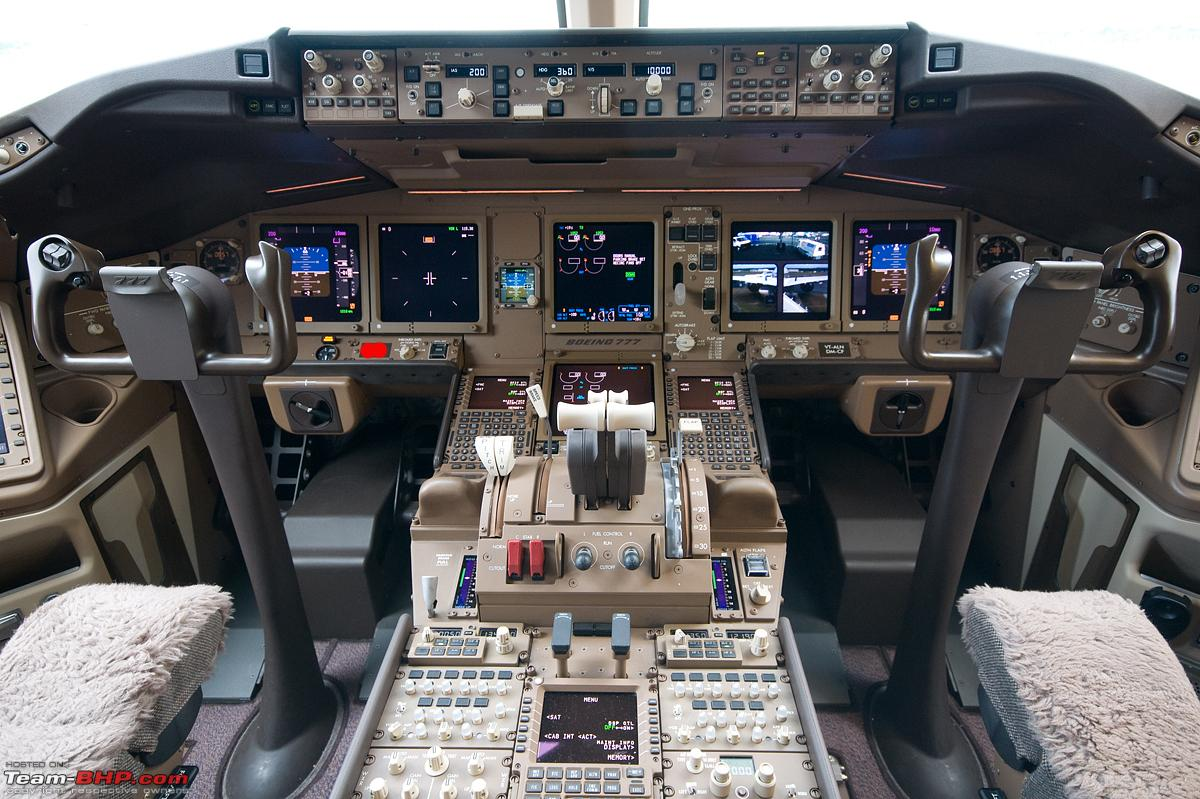
\includegraphics[width=0.95\textwidth]{01.tablero.instrumentos/U01.imagenes/1.2.distribucion.normalizada.instrumental.en.tablero/01-boeing777cockpit.jpg}

    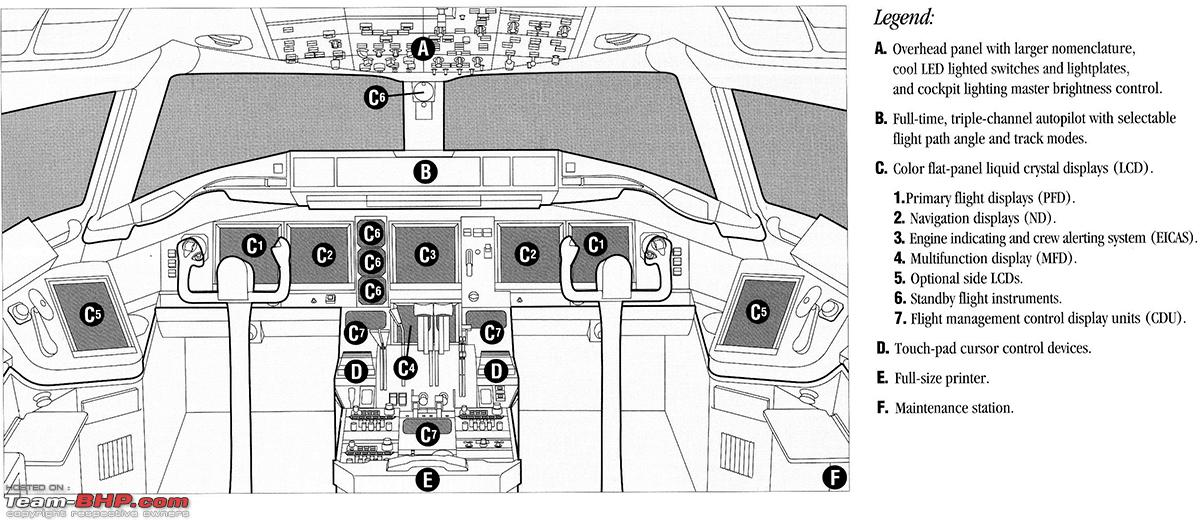
\includegraphics[width=0.95\textwidth]{01.tablero.instrumentos/U01.imagenes/1.2.distribucion.normalizada.instrumental.en.tablero/01-boeing777_cockpitlayout.jpg}   
  \caption{Cabina del Boeing 777 \protect\cite{Boeing777_cabina}}
  \label{fig:01.cabina.boeing.777}
\end{figure}



%https://pmflight.co.uk

\begin{figure}[!htb]
  \centering
    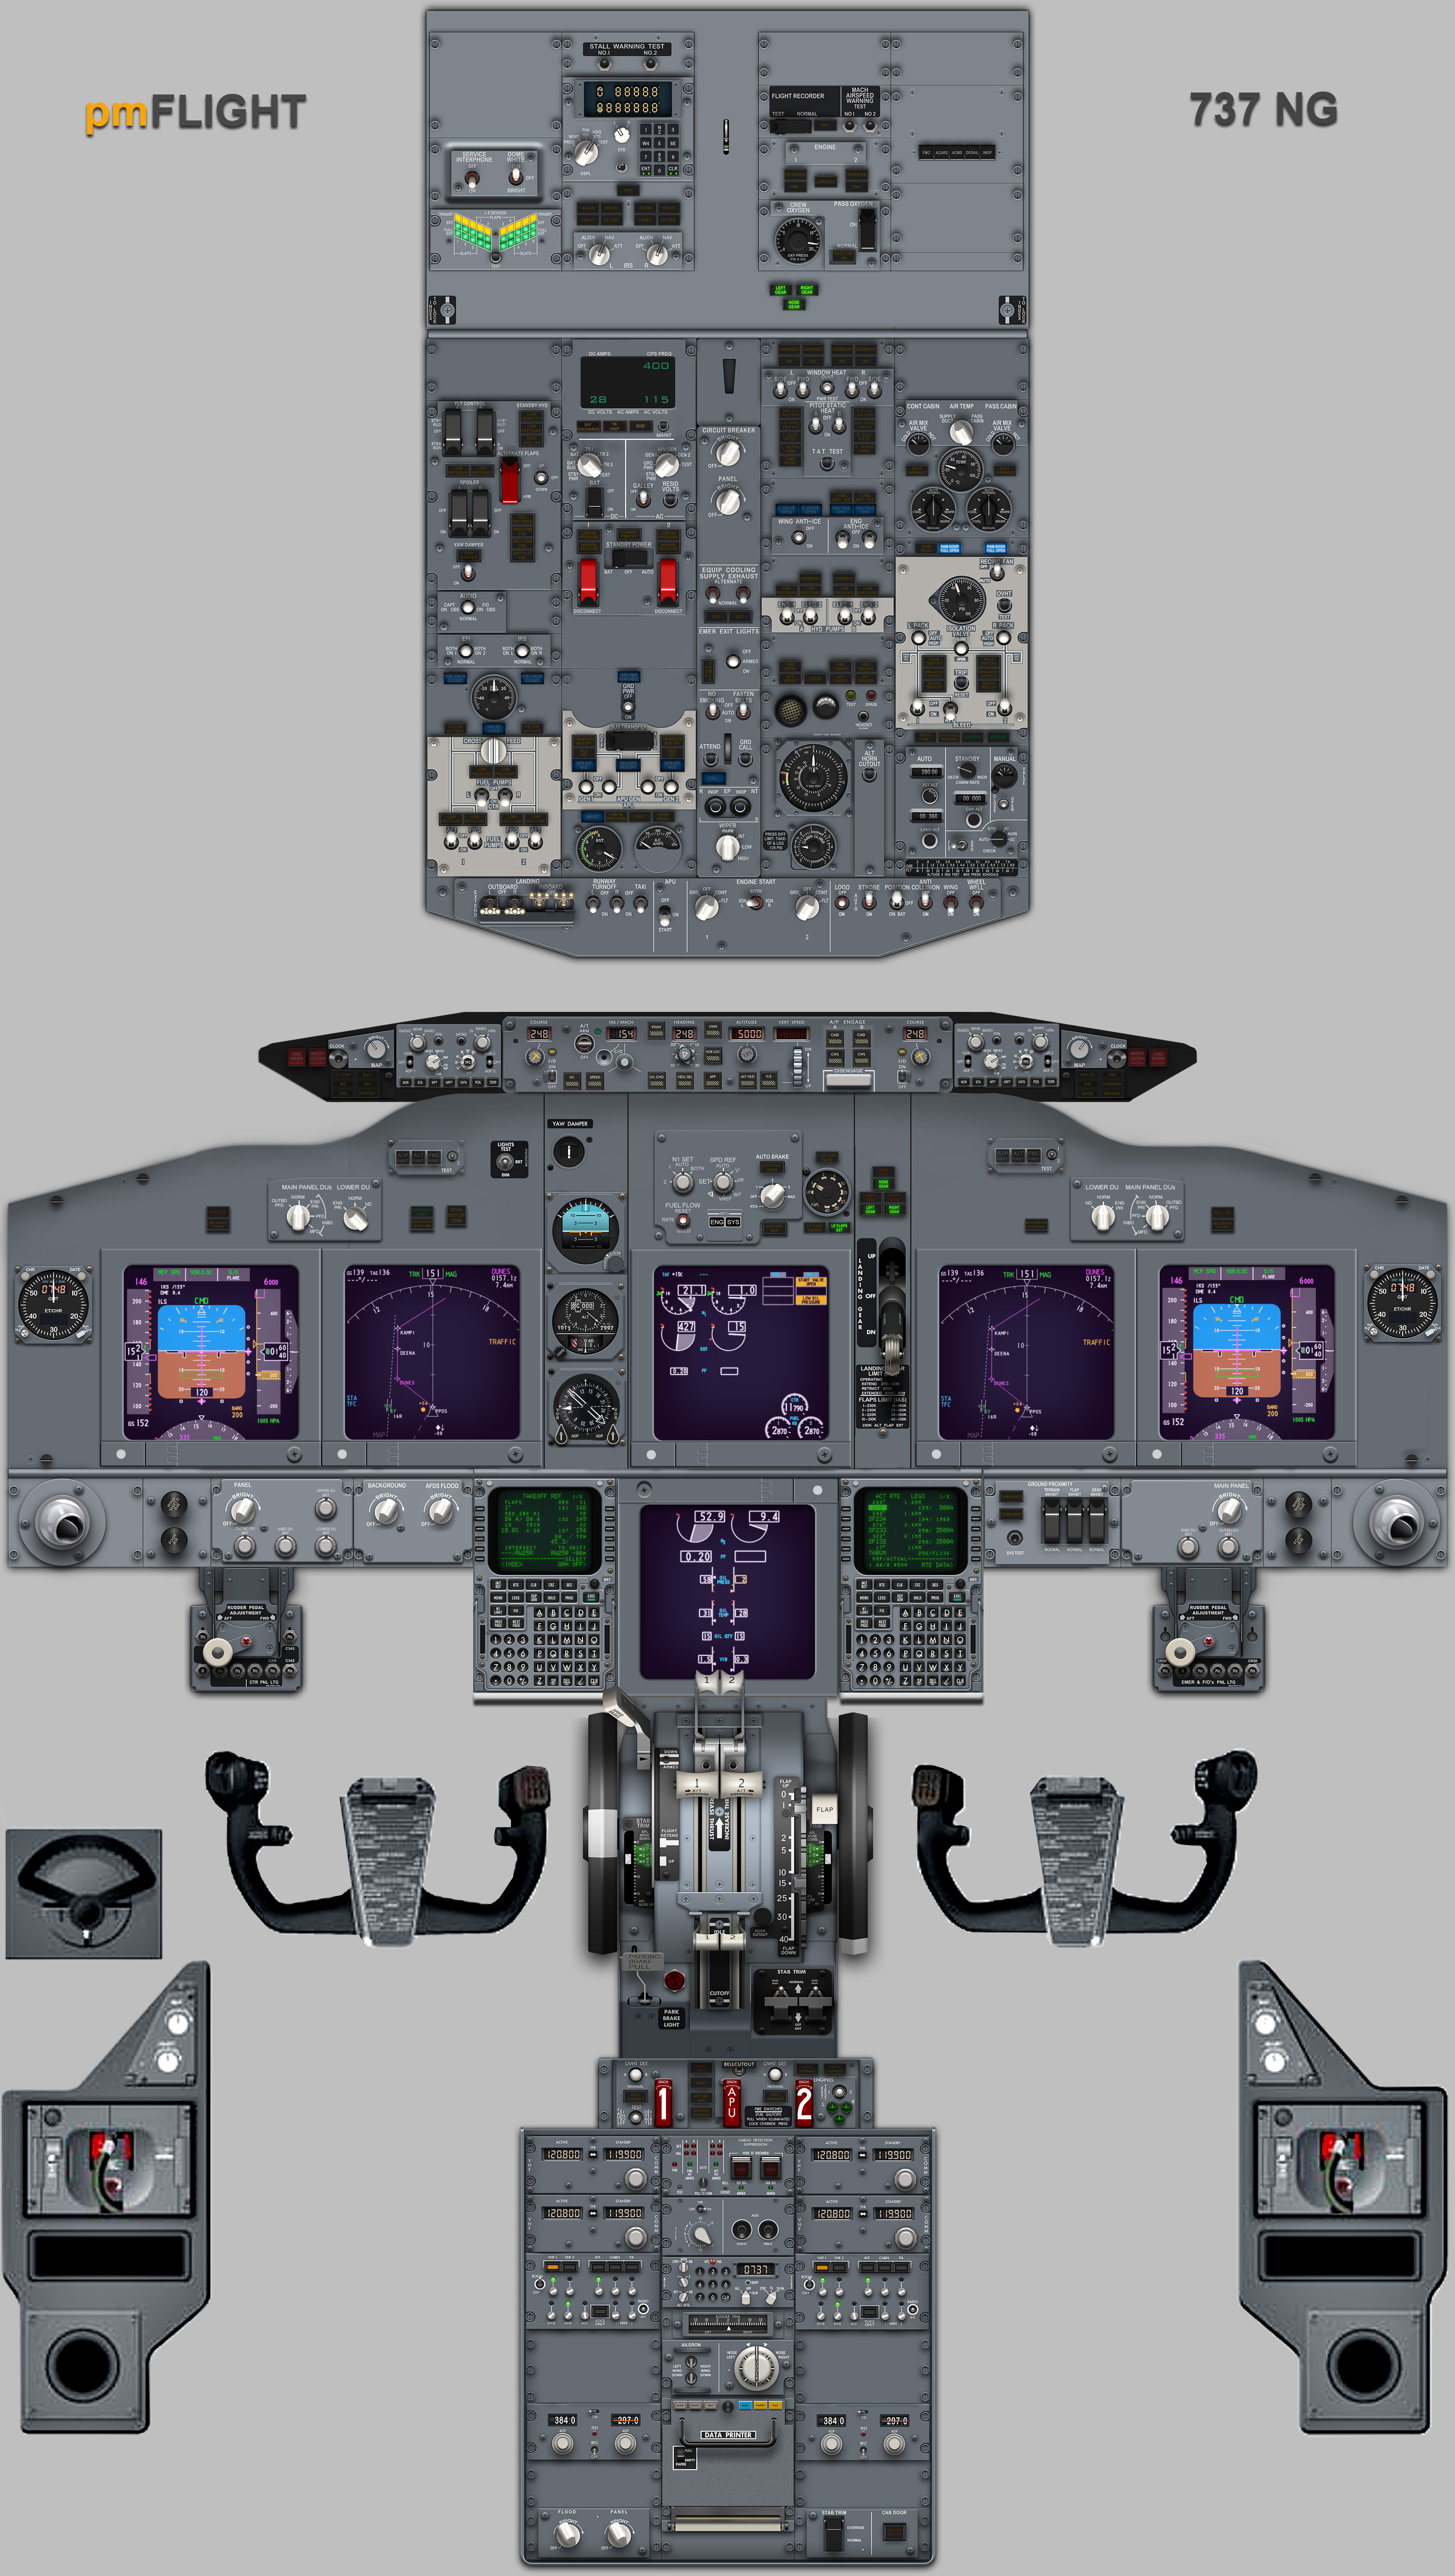
\includegraphics[width=0.6\textwidth]{01.tablero.instrumentos/U01.imagenes/1.2.distribucion.normalizada.instrumental.en.tablero/01-free-737-poster-HI.jpg}

  \caption{Cabina del Boeing 737 NG. Gentileza \protect\href{https://pmflight.co.uk}{pmFlight}}
  \label{fig:01.cabina.boeing.737NG}
\end{figure}

\begin{figure}[!htb]
  \centering
    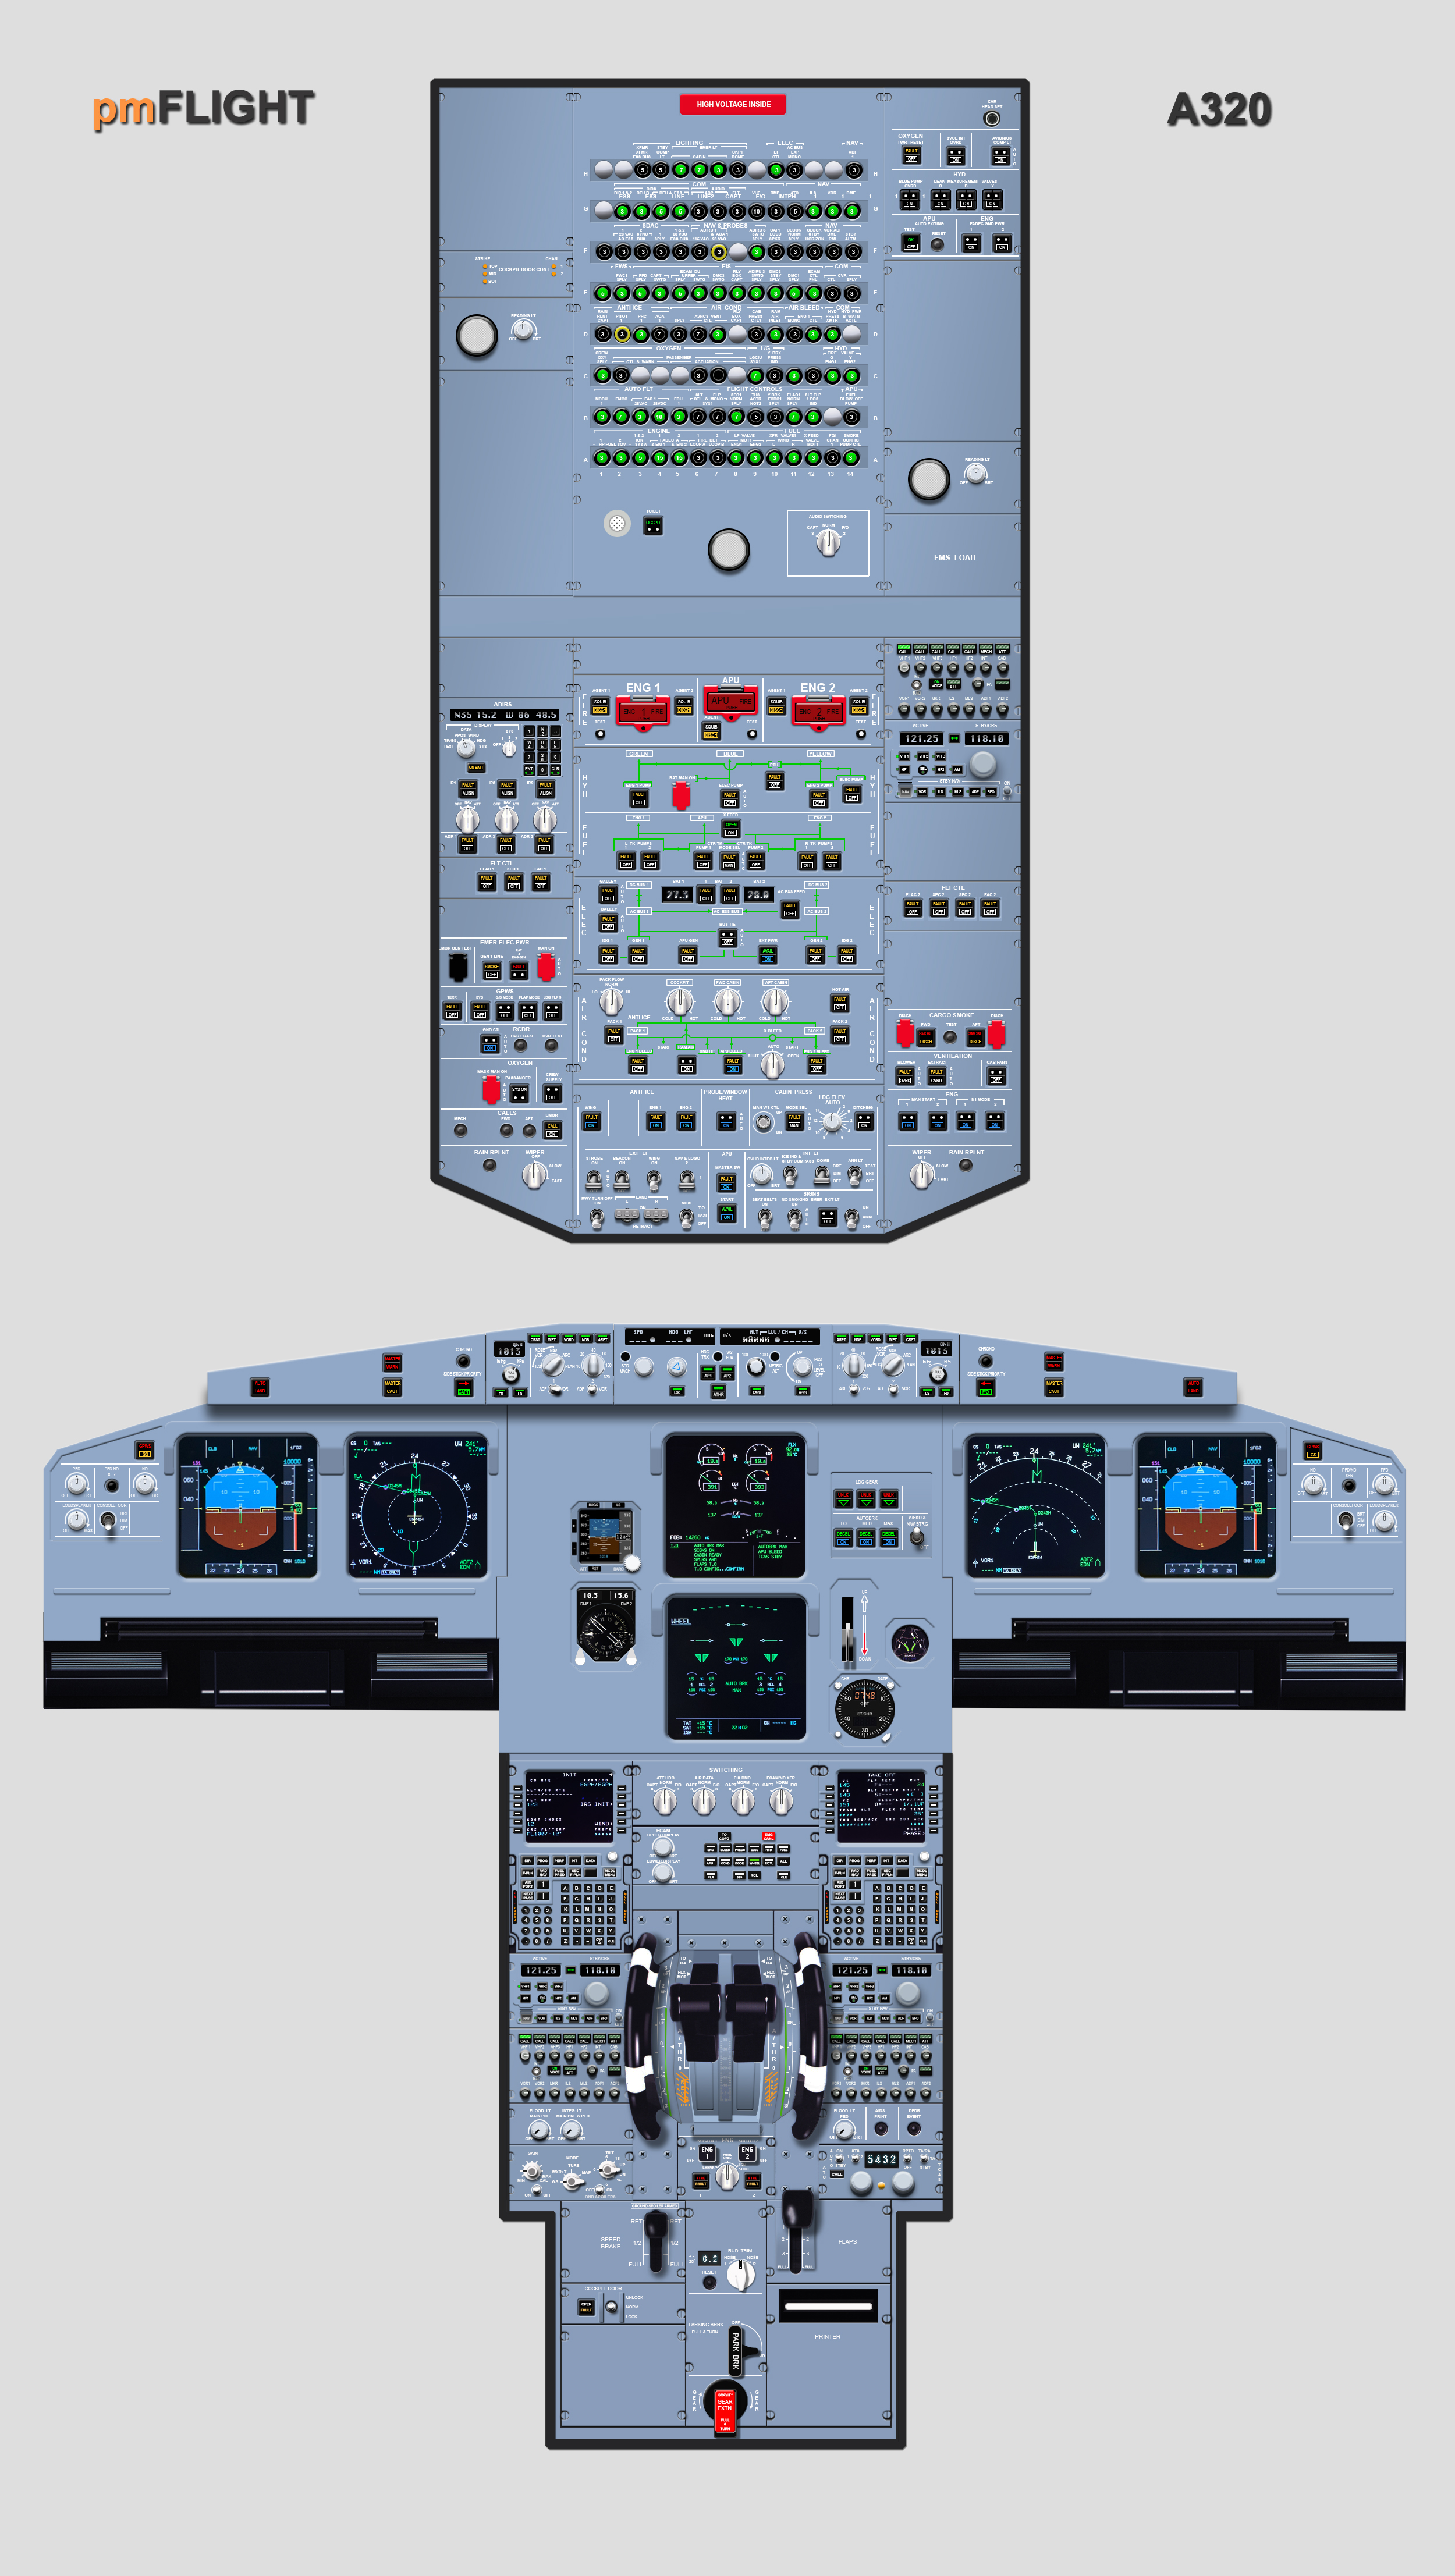
\includegraphics[width=0.6\textwidth]{01.tablero.instrumentos/U01.imagenes/1.2.distribucion.normalizada.instrumental.en.tablero/01-free-airbus-a320-poster-HI.jpg}

  \caption{Cabina del Airbus A320. Gentileza \protect\href{https://pmflight.co.uk}{pmFlight}}
  \label{fig:01.cabina.boeing.A320}
\end{figure}




\section{Presentaci\'on en Pantalla Electr\'onica}
\label{sec:presentacion.en.pantalla.electronica}

{Un poco de historia...}


        \begin{description}
        \item[1970] NASA investigaci\'on en como mostrar instrumentos
          de vuelo
        \item[1982]Boeing 767 con pantallas electr\'onicas de datos tipo \ac{CRT}
        \item[1990]Fines de la d\'ecada, pantallas \ac{LCD} reemplazan
          pantallas \ac{CRT}, ver Figura \ref{fig:01.CRT}.
        \item[Actualidad] La mayor\'ia de las aeronaves equipadas con
          pantallas \ac{LCD}, ver Figura \ref{fig:01.LCD}.
        \item[Futuro] Uso de pantallas tipo \ac{OLED} y empleo de pantallas t\'actiles, ver Figura \ref{fig:01.04.cabina.actual.vs.cabina.futura} y Figura \ref{fig:01.OLED}.
        \end{description}

        \begin{figure}
          \centering
          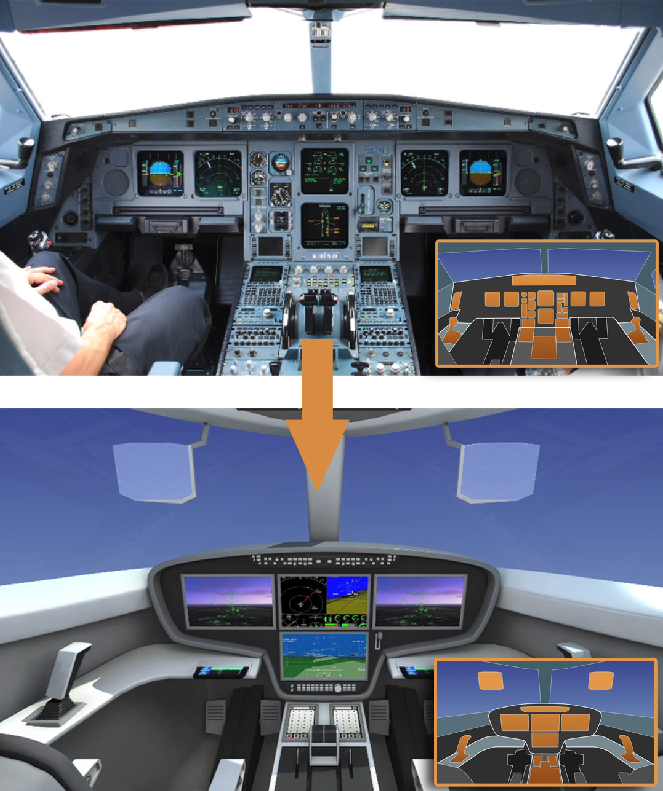
\includegraphics[width=0.8\linewidth]{01.tablero.instrumentos/imagenes/1.4.pantalla.electronica/01_04_cabina_actual_vs_cabina_futura.png}
          \caption{Cabina actual y cabina futura con pantallas t\'actiles \protect\cite{Bonelli2011FlyingWC}}
          \label{fig:01.04.cabina.actual.vs.cabina.futura}
        \end{figure}


\begin{tcolorbox}
La empresa Thales ha presentado FlytX, la nueva generaci\'on de cabina de vuelo con pantallas t\'actiles para aeronaves y helic\'opteros, mayor informaci\'on puede encontrarse 
\href{https://www.thalesgroup.com/en/markets/aerospace/flight-deck-avionics-equipment-functions/flytx-tactile-large-display-flight-deck}{aqu\'i} 
y un video de la misma 
\href{https://www.youtube.com/watch?v=PcrEUL8ATgE}{aqu\'i}.
\end{tcolorbox}

\begin{figure}[!htb]
  \centering
  \subfigure[CRT]{\includegraphics[width=0.75\linewidth]{01.tablero.instrumentos/imagenes/1.4.pantalla.electronica/CRT.gif} \label{fig:01.CRT}}

  \subfigure[LCD]{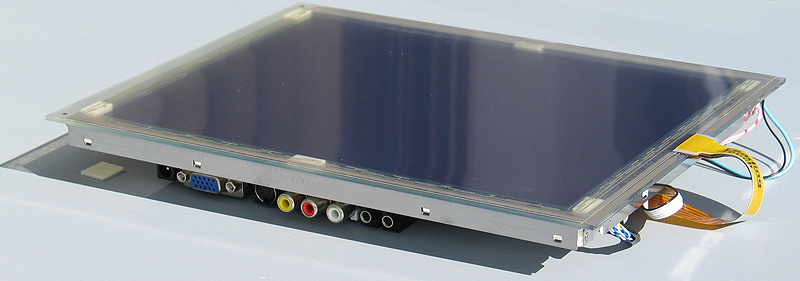
\includegraphics[width=0.45\linewidth]{01.tablero.instrumentos/imagenes/1.4.pantalla.electronica/LCD.jpg} \label{fig:01.LCD}}
  \subfigure[OLED]{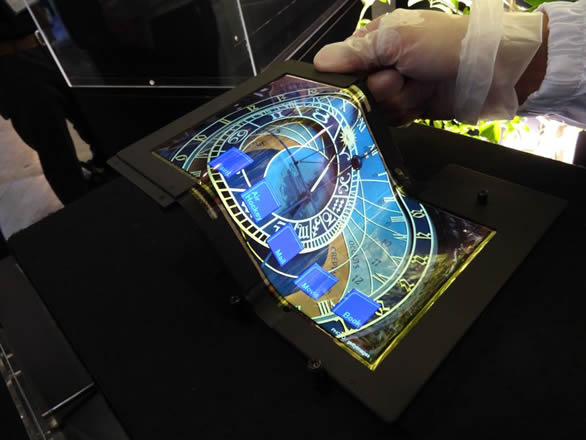
\includegraphics[width=0.45\linewidth]{01.tablero.instrumentos/imagenes/1.4.pantalla.electronica/foldable-oled-display.jpg} \label{fig:01.OLED}}
  
  \caption{Diferentes tipos de tecnolog\'ia de pantallas}
\label{fig:01.diferentes.tecnologias.pantallas}
\end{figure}



  \subsection{ \ac{EIS}}
  \label{sec:01.EIS}

  El sistema comprende el \ac{EFIS} y al \ac{ECAM}  tal como se muestra en la Figura \ref{fig:01.eis}. 

  \begin{figure}[!htb]
    \centering
    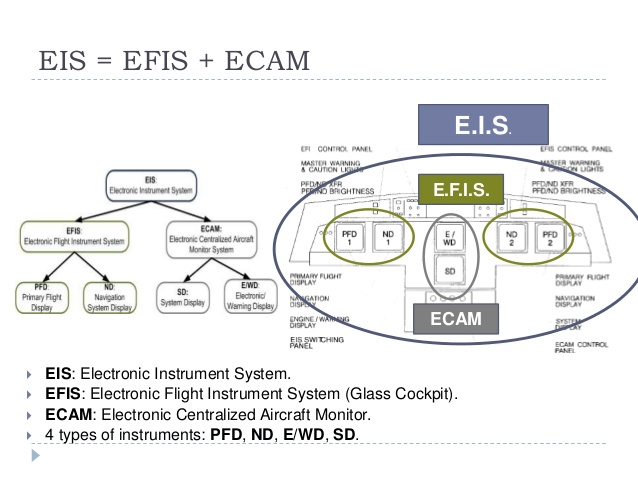
\includegraphics[width=\textwidth]{01.tablero.instrumentos/U01.imagenes/1.4.pantalla.electronica/01_eis.jpg}
    \caption{EIS}
    \label{fig:01.eis}
  \end{figure}

%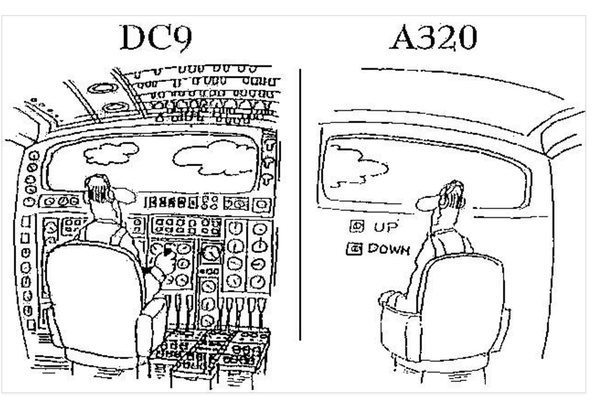
\includegraphics[width=0.5\textwidth]{01.tablero.instrumentos/imagenes/1.4.pantalla.electronica/efis_humor.png}


% Ejemplos:

% 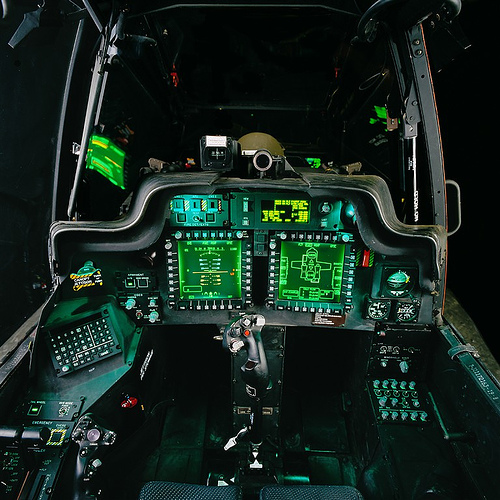
\includegraphics[width=0.34\textwidth]{01.tablero.instrumentos/imagenes/1.4.pantalla.electronica/apache.jpg}
% \hspace{3mm}
% 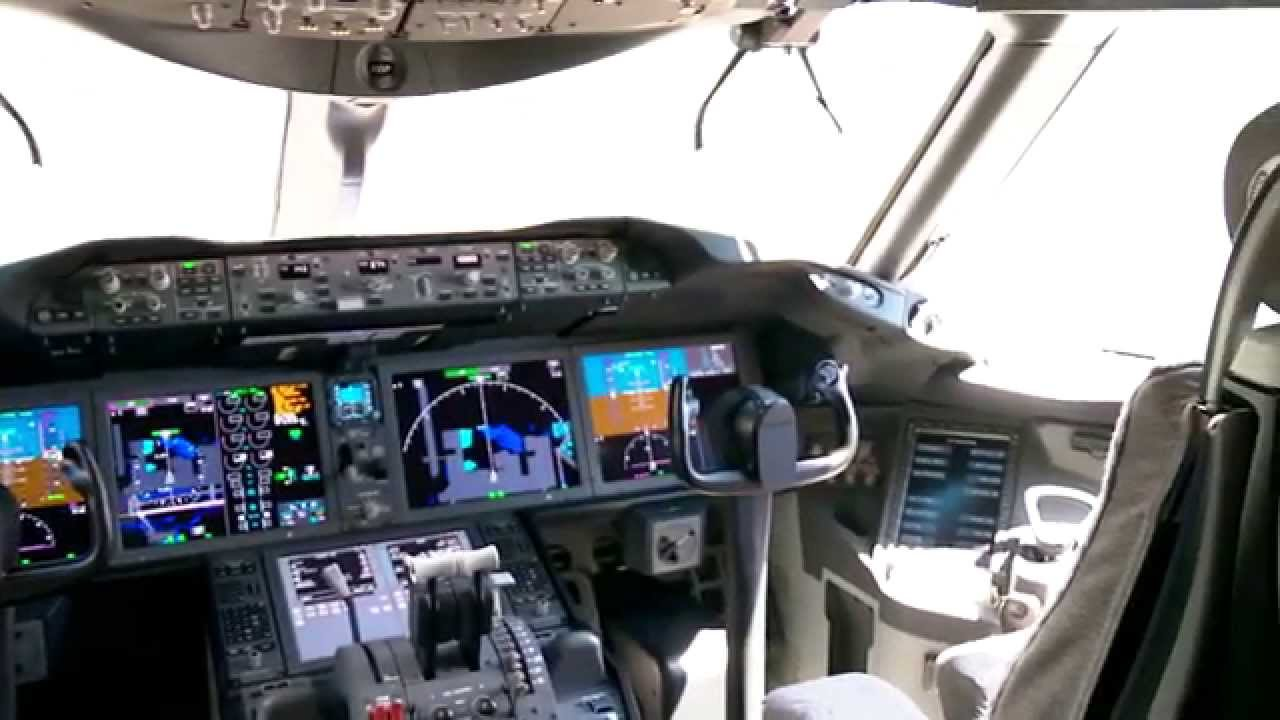
\includegraphics[width=0.55\textwidth]{01.tablero.instrumentos/imagenes/1.4.pantalla.electronica/dreamliner.jpg}

% Helic\'optero Apache \hspace{25mm} Boeing 787 Dreamliner


Una instalaci\'on \ac{EIS} sigue la secuencia siguiente:

\vspace{3mm}


 Pantallas \qquad $\Longrightarrow$ \qquad
 Controles  \qquad $\Longrightarrow$ \qquad
 Procesadores de datos 

 \begin{tcolorbox}
   El sistema EIS est\'a brevemente explicado  
   \href{https://www.youtube.com/watch?v=AS91uq1tkjQ}{aqu\'i} y \href{https://www.youtube.com/watch?v=2aix7kIL29o}{en este video}
 \end{tcolorbox}


\subsection{EFIS}
\label{sec:01.efis}


Como ejemplo de \ac{EFIS} se tiene el producto 
\href{http://www.ifd-net.com/}{IFD-NET EFIS de M.A.V.AVIONIC DIVISION}  que proveen un manual de especificaciones del producto y de instalaci\'on.


Video interesante con detalle de uso de la cabina de un Airbus 350 
\href{https://www.youtube.com/watch?v=jk-WClye4bw}{Airbus A350 Lufthansa ULTIMATE COCKPIT MOVIE + Business Class Tokyo [AirClips full flight series]}


\subsubsection{\ac{PFD}}
\label{sec:01.pfd}

	El PFD reemplaza a los seis (6) instrumentos tradicionales.
	Muestra la informaci\'on cr\'itica de vuelo 
	incluyendo velocidad, altitud,direcci\'on (heading)
	actitud y velocidad vertical.

	Est\'a dise\~nado para mejorar las alertas al piloto
	al integrar informaci\'on en una sola pantalla.
	Reduce el tiempo para monitorear otros instrumentos.

	Alerta a los pilotos de condiciones potencialmente peligrosas
        cambiando el color o la forma en el display o mediante alertas
        de sonido (baja velocidad, alta tasa de descenso). 

        \begin{figure}[!htb]
          \centering
          \subfigure[PFD]{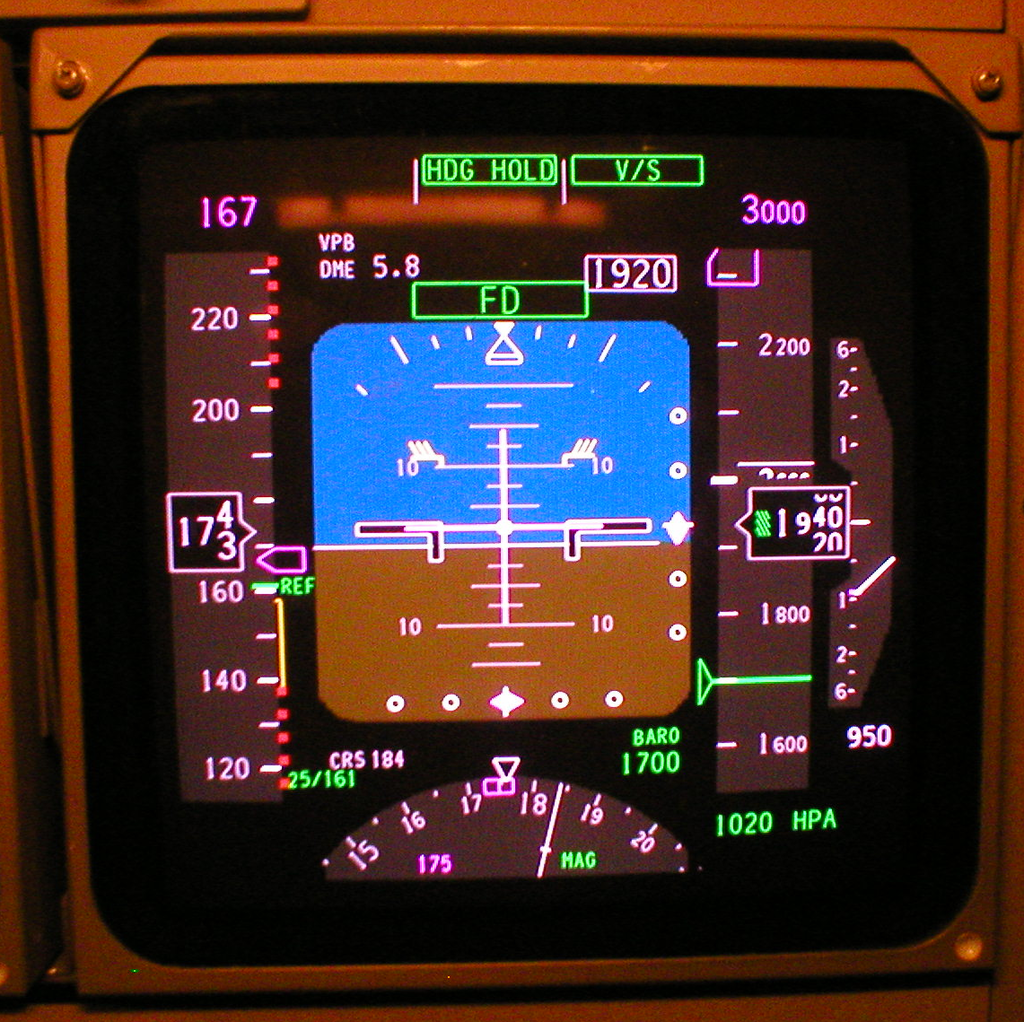
\includegraphics[width=0.45\textwidth]{01.tablero.instrumentos/U01.imagenes/1.4.pantalla.electronica/Primary_Flight_Display,_Boeing_747-400.png}
          }
          \subfigure[PFD]{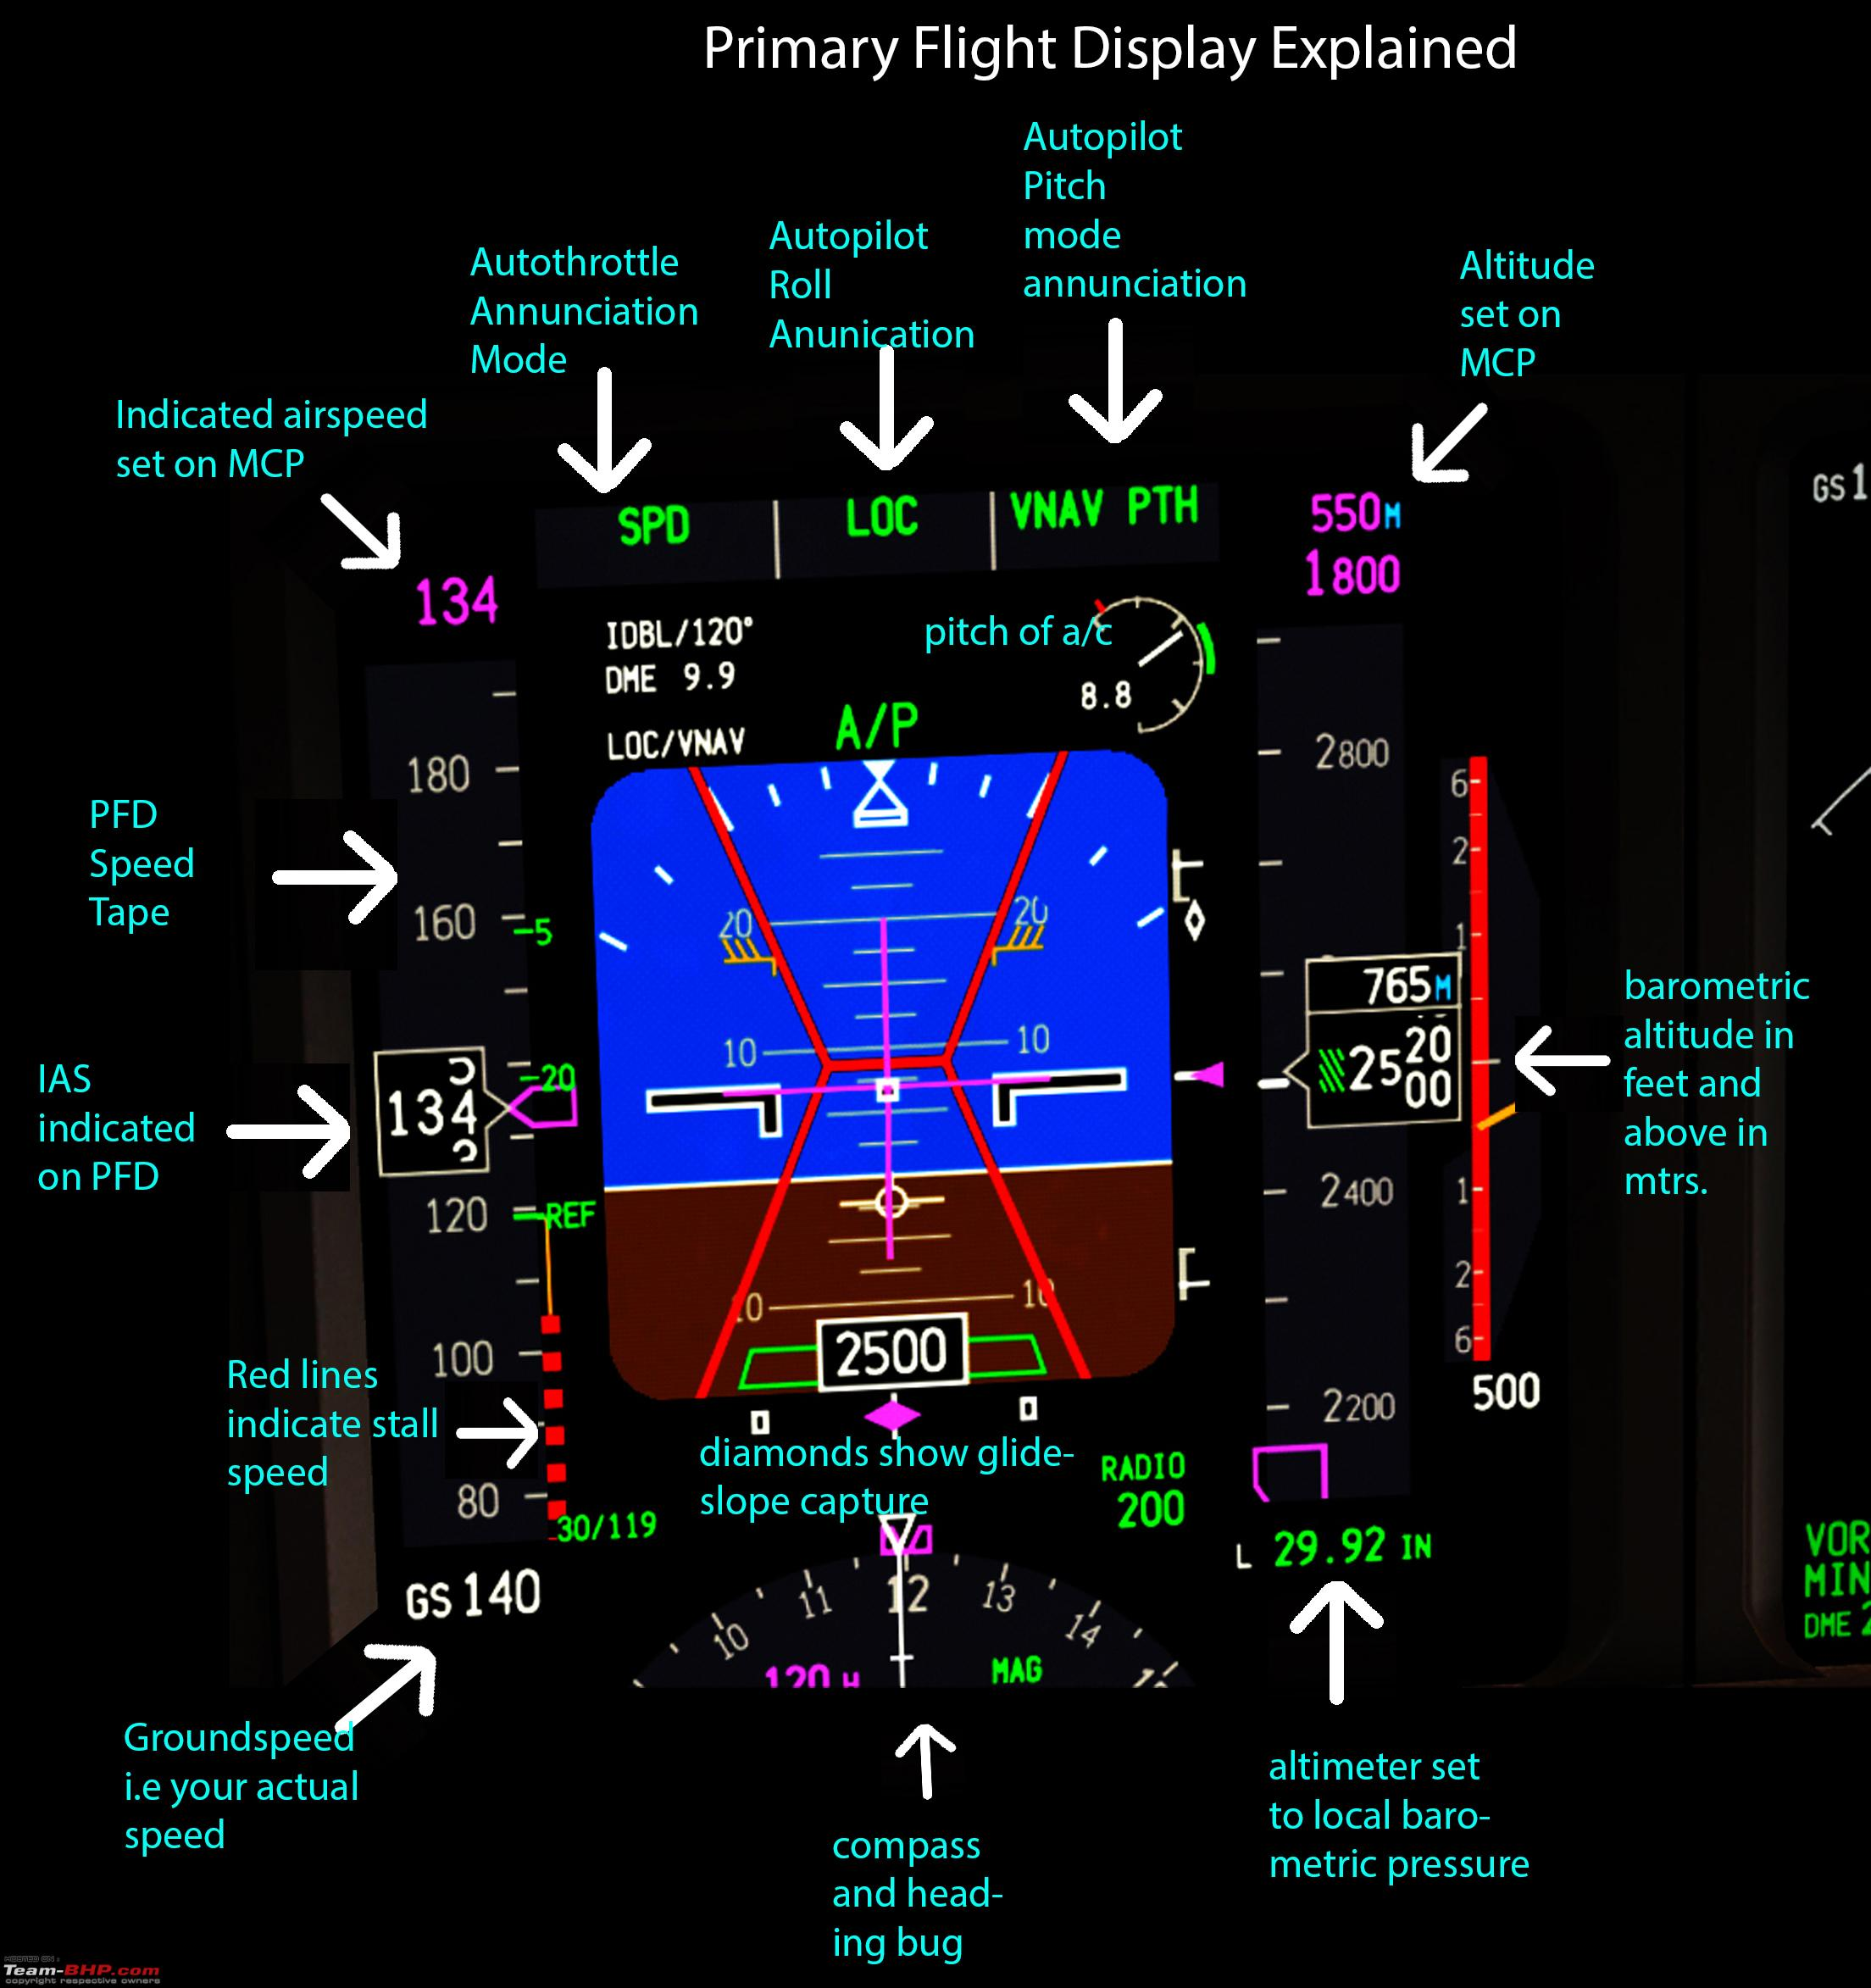
\includegraphics[width=0.45\textwidth]{01.tablero.instrumentos/U01.imagenes/1.4.pantalla.electronica/01_pfd_explanation.jpg}
          }
          
          \caption{PFD}
      \label{fig:01.pfd}
    \end{figure}


\subsubsection{\ac{ND}}
\label{sec:01.nd}

Tambi\'en es conocida como \ac{MFD}

    Provee informaci\'on para navegaci\'on (VOR, DME, ILS), iInformaci\'on clim\'atica de m\'ultiples sistemas (radar a bordo, sensores de detecci\'on de rel\'ampagos).

    Idem al PFD el MFD puede cambiar color, forma y dar alertas  sonoras.

    \begin{figure}[!htb]\centering
      
      \includegraphics[width=0.45\textwidth]{01.tablero.instrumentos/U01.imagenes/1.4.pantalla.electronica/Navigation_Display_(ND)_on_Boeing_747-400.jpg}
      
      \caption{MFD o ND}
  \label{fig:01.MFD}
\end{figure}

\subsubsection{\ac{FMS}}
\label{sec:01.FMS}

   Instrumentos para mantener el plan de vuelo (flight plan) permite
    a los pilotos modificarlo en vuelo

    Dada la posici\'on y el plan de vuelo, el  \ac{FMS} se encarga de guiar
    el avi\'on a lo largo del mismo, gestiona los diversos factores
    que afectan al vuelo del avi\'on, tanto la ruta que tiene que
    seguir, como los niveles \'optimos a los cuales volar para reducir
    el consumo y hacer un vuelo m\'as eficiente.


    Usualmente se presenta como una pantalla peque\~na y un teclado

    El \ac{FMS} se compone principalmente del \ac{CDU} y 
    el \ac{FMC}
 
El piloto introduce los datos al \ac{FMC} a trav\'es de la \ac{CDU} que no es m\'as que un teclado 
y una pantalla que sirve para la comunicaci\'on entre el piloto y el \ac{FMC}. 
A trav\'es de la \ac{CDU} el piloto programa la ruta del vuelo, las \ac{SID}  
y las \ac{STAR}, as\'i como los puntos en las rutas donde el avi\'on debe ascender 
a niveles \'optimos seg\'un disminuye el peso del avi\'on.

\begin{figure}[!h]
  \centering
  \includegraphics[width=0.9\textwidth]{01.tablero.instrumentos/imagenes/1.4.pantalla.electronica/fms_plan_vuelo.jpg}
   \caption{FMC}
\label{fig:01.FMC}
\end{figure}

El \ac{FMC} adem\'as adquiere datos de muchos de los sistemas del avi\'on. Para empezar recibe informaci\'on de los inerciales, y de los \ac{GPS} para triangular la posici\'on del avi\'on y tener una posici\'on a\'un m\'as exacta de donde se encuentra el avi\'on.

El \ac{FMS} tiene principalmente dos bases de datos. Una base de datos de navegaci\'on, donde est\'an almacenadas las rutas, aerov\'ias, \ac{SID}, \ac{STARS}, as\'i como las frecuencias de las radio ayudas a la navegaci\'on que va a sintonizar autom\'aticamente a lo largo de la ruta. Esta base de datos se renueva cada 28 d\'ias para poder estar actualizada cuando se producen cambios en los espacios a\'ereos o se modifican procedimientos de aproximaci\'on. 
El \ac{FMC} es capaz de guardar dos (2)  bases de datos de navegaci\'on.

La otra base de datos es de performance del avi\'on. Esta base de datos contiene informaci\'on de los niveles \'optimos de vuelo dependiendo del peso del avi\'on. Los consumos que tiene el avi\'on para cada peso y nivel de vuelo. Las predicciones de ascenso y descenso del avi\'on.

Como el avi\'on va envejeciendo a lo largo de su vida y disminuyendo sus performance, el \ac{FMS} admite un valor de degradaci\'on de las performance que se introduce en la p\'agina principal del \ac{CDU} para que de unas previsiones de combustibles m\'as reales seg\'un el avi\'on se va haciendo ``mayor''

Con el tiempo el \ac{FMS} ha ido mejorando y abarcando nuevas posibilidades. As\'i Airbus cambia el nombre 
al \ac{CDU} y le ha pasado a llamar \ac{MCDU}. Ahora no solamente se puede acceder 
al \ac{FMC} a trav\'es del teclado de la \ac{CDU} si no a una infinidad de nuevos servicios.

Mediante el \ac{MCDU} se accede al \ac{ATSU}, \ac{AIDS}, \ac{CFDS} y al \ac{FMS} 
comentado hasta ahora y llamado por Airbus \ac{FMGS}.

\begin{itemize}
\item El \ac{ATSU} es el acceso al Acars o sistema de comunicaciones
  tanto con la compa\~n\'ia como con el control a\'ereo. A trav\'es de
  esta opci\'on se recibe desde la hoja de carga, cualquier mensaje
  escrito que envie la compa\~n\'ia, hasta la autorizaci\'on para
  ingresar a otro pa\'is.

\item   El \ac{CFDS} es usado principalmente por el personal de
  mantenimiento.  En el est\'an los reportes de mantenimiento del
  vuelo, y las aver\'ias que haya tenido el avi\'on, por muy
  peque\~nas o temporales que hayan sido (aunque haya sido un fallo
  temporal de cualquier fusible por menos de 1 sg se queda
  registrado).

\item   El \ac{AIDS} es otra herramienta que maneja mantenimiento, sirve
  para interrogar y realizar TEST a cualquier sistema del avi\'on para
  conocer en qu\'e estado de operatividad se encuentra.
\end{itemize}


\begin{figure}[!h]
  \centering
  \includegraphics[width=0.9\textwidth]{01.tablero.instrumentos/imagenes/1.4.pantalla.electronica/mcdu.jpg}
  \caption{MCDU}
\label{fig:01.MCDU}
\end{figure}

\subsection{EICAS y ECAM}
\label{sec:01.eicas+ecam}

El \ac{EICAS} ha sido desarrollado por Boeing para proporcionar toda la instrumentación del motor y anuncios de tripulación en un formato integrado, 
por otra parte, el sistema utilizado en los aviones Airbus es el \ac{ECAM}. 
Los dos sistemas operan con filosof\'ias diferentes: ambos sistemas producen mensajes de advertencia, precaución y aviso que deben ser evaluados por la tripulación; en ciertos casos, el sistema indica los procedimientos necesarios para abordar el problema. 
Cada sistema utiliza  pantallas LCD o  CRT,  sus funciones básicas son monitorear los sistemas de la aeronave y mostrar información relevante a los pilotos. En la Figura \ref{fig:eicas+ecam} puede apreciarse la presentaci\'on de dichos sistemas.


\begin{figure}[!h]
  \centering
  \subfigure[EICAS en cabina de Boeing 747-400 \protect\cite{747-400-cabina}]{\includegraphics[width=0.45\textwidth]{01.tablero.instrumentos/imagenes/1.4.pantalla.electronica/01_Boeing_747-400_cockpit.jpg}}
  \subfigure[ECAM \protect\cite{NASA_Mumaw}]{\includegraphics[width=0.45\textwidth]{01.tablero.instrumentos/imagenes/1.4.pantalla.electronica/Airbus-ECAM-displays_W640.jpg}}
  \caption{EICAS y ECAM}
  \label{fig:eicas+ecam}
\end{figure}


EICAS est\'a dividido en  dos pantallas: Upper EICAS ( superior) y Lower EICAS ( inferior),  
en la Tabla \ref{tab:01.eicas.presentacion.en.pantallas} se detalla la informaci\'on presentada en cada pantalla.% Conocido así por pilotos de un 747.
Este sistema provee la instrumentación de diversos parámetros del motor, por ejemplo RPM, valores de temperatura, caudal y cantidad de combustible, presión de aceite, etc. 
Los otros sistemas de la aeronave controlados por EICAS son; hidráulica, neumática, eléctrica, de deshielo, control de los sistemas de superficie. 
Mediante este sistema se sustituye a todos los medidores analógicos con software impulsado por pantallas electrónicas.

\begin{table}[!h]\centering
\caption{EICAS presentaci\'on en sus pantallas}
\label{tab:01.eicas.presentacion.en.pantallas}
  
\begin{tabular}{m{0.3\textwidth}m{0.65\textwidth}} \hline \rowcolor{yellow!30}
{\bf Pantalla} & {\bf Funciones } \\ \hline
\parbox{\linewidth}{  \textbf{Pantalla Superior} \\
(Upper EICAS)
}
& Muestra datos basicos de motor, indicador del modo de potencia, 
lista de mensajes de alerta, 
conjunto de arranque en vuelo, 
tren de aterrizaje, 
flaps,
combustible,
presi\'on en los conductos de aire,
altura de la cabina. \\ \rowcolor{cyan!30}

\parbox{\linewidth}{  \textbf{Pantalla Inferior} \\ Lower EICAS}
& 
La característica principal de esta
pantalla es que tiene la flexibilidad
permitir seleccionar distintos grupos
de datos en dos formas básicas:
\textcolor{blue}{\it Datos en Cifras}, y
\textcolor{blue}{\it Cuadros Sin\'opticos}.
Tambi\'en muestra mensajes de estado. \\ \hline
\end{tabular}
\end{table}

%\href{https://docplayer.es/21099386-L-aeroteca-c-montseny-num-22-esquina-sant-joaquim-08012-barcelona-telefono-932-181-739-www-aeroteca-com-www-simutaca-com.html}{BAJAR INFORMACIÓN DE AQUÍ PARA COMPLETAR EL APUNTE}

Los cuadros sinopticos de sistemas son presentados en la Lower EICAS, consisten en esquemas que representan diferentes sistemas de la aeronave.  Se les conoce como ``{\it toy modeling}'' (modelos de juegete) y permiten a los pilotos comprobar con una mirada a la pantalla de que forma est\'an dispuestos los comandos de varios sistemas. 

\begin{myboxAzul}{}
  El sistema EICAS avisa al piloto de cualquier problema usando la
  sección de mensajes de ALERTA del EICAS SUPERIOR.  El color del
  mensaje varía según su importancia:

  \begin{itemize}
  \item \textcolor{red}{\bf ROJO} indica máximo nivel de peligro y se
    denomina WARNING.

  \item \textcolor{amber}{\bf AMBAR} es el siguiente nivel, de
    precaución, y se denomina CAUTION

  \item El ultimo nivel corresponde a simples AVISOS y puede ser de
    color \textcolor{amber}{\bf AMBAR} o {\bf BLANCO} \mbox{(STATUS)}.
  \end{itemize}
\end{myboxAzul}

Los WARNING y CAUTION no pueden cancelarse

Los mensajes pueden ir acompañados por
señales ACUSTICAS.

Los mensajes STATUS del EICAS indican problemas
que pueden afectar la capacidad de funcionamiento correcto
del avión y son distintos de los mensajes ALERT.

\begin{myboxAzul}{EICAS}
  \href{https://www.youtube.com/watch?v=wSgB9FoSR5E}{
    \includegraphics[height=1cm]{imagenes.iconos/video.jpg}
  } Video explicando como funciona EICAS.
\end{myboxAzul}

ECAM proporciona las características principales de EICAS pero también muestra las acciones correctivas que debe tomar la tripulación así como las limitaciones del sistema después de las fallas. 

Usando una jerarquía codificada por colores, la tripulación puede asimilar la información que se presenta y tomar las medidas correctivas necesarias. 
ECAM se introdujo por primera vez en el Airbus A320. En la Figura pueden observarse varias pantallas de presentaci\'on de ECAM.

ECAM comprende una serie de sistemas integrados que muestran información a la tripulación de manera eficiente. los sensores de aeronaves se clasifican en funciones clave de supervisión; estos sensores transmiten datos a dos \ac{SDAC}. Los datos se procesan y se envían a dos  \ac{FWC} que están programadas para identificar cualquier inconsistencia en los datos y luego emitir los datos a través de tres \ac{DMC}.

Si se detecta una falla o evento del sistema, uno de los FWC genera los mensajes de advertencia y alertas auditivas apropiados. Los sistemas críticos, como el motor y la cantidad de combustible, se env\'ian directamente a las FWC para que aún puedan ser monitoreados en caso de falla de ambos SDAC. 

ECAM puede tolerar la falla de un SDAC y un FWC y seguir operando. La informaci\'on es presentada en dos pantallas, una por arriba de la otra, en la Tabla \ref{tab:01.ecam.presentacion.en.sus.pantallas} se detalla la informaci\'on presentada en cada pantalla.

\begin{table}[!h]
  \centering
\caption{ECAM presentaci\'on en sus pantallas}
\label{tab:01.ecam.presentacion.en.sus.pantallas}

  \begin{tabular}{m{0.3\textwidth}m{0.65\textwidth}} \hline \rowcolor{yellow!30}
{\bf Pantalla} & {\bf Funciones } \\ \hline
  \parbox{\linewidth}{\textbf{Pantalla Superior} \\
  \ac{EWD}} 
& Muestra los principales datos del motor y otras informaciones: por ejemplo, configuración de los flaps y slats, EOR, \ac{EGT}, N1 y N2 , FUEL FLOW, mensajes y checklist en relación a operaciones normales. \\ \rowcolor{cyan!30}
  \parbox{\linewidth}{\textbf{Pantalla Inferior} \\
  \ac{SD}}
   & Presenta avisos permanentes de información adicional,  ya sea de forma automática o manual, lo cual incluye daños del sistema y sus consecuencias.  Se muestra: Indicaciones adicionales del motor, es decir, combustible utilizado, nivel de aceite, presión y temperatura de aceite niveles de vibración del motor y aviso de obstrucción de filtros de aceite y del combustible. Ademas de página de crucero, Sistema neumático, sangrando e aire ( bleed air), Sist. eléctrico, Sist. hidráulico, presurización de cabina, Sist. de combustible, APU, aire acondicionado, puertas y sistema de oxigeno, mandos de vuelo, tren de aterrizaje. \\ \hline
\end{tabular}

\end{table}

%El sinóptico típico de un sistema eléctrico se muestra en la figura 14.9. En esta ilustración, se muestran gráficamente las fuentes de energía que suministran barras colectoras específicas, junto con información como los voltajes de la batería y la unidad rectificadora del transformador (TRU) y las corrientes de suministro. La capacidad del generador se muestra como un porcentaje del máximo, junto con el voltaje y la frecuencia de salida.

Las fallas del sistema de la aeronave se priorizan como fallas de nivel 1, 2 o 3 para la pantalla superior y / o inferior. En la Tabla \ref{tab:01.ecam.jerarquia.de.advertencias.y.precauciones} se detalla la jerarquía de advertencias y precauciones.

\begin{table}[!h]
 \centering
 \caption{ECAM jerarqu\'ia de advertencias y precauciones}
 \label{tab:01.ecam.jerarquia.de.advertencias.y.precauciones}

  \begin{tabular}{m{0.10\textwidth}m{0.3\textwidth}m{0.2\textwidth}m{0.3\textwidth}} \hline \rowcolor{cyan!20}
\centering {\bf Jerarqu\'ia} & \centering {\bf Descripci\'on} & \centering {\bf Ejemplo} & \multicolumn{1}{c}{\bf Indicaci\'on} \\ \hline 

 \cellcolor{red!80} \centering \textcolor{white}{\bf Fallas de nivel 3} 
&
\begin{spacing}{0.75}
  {\scriptsize Situaciones que requieren una acción inmediata de la tripulación e indican que la aeronave está en peligro. }
\end{spacing}
& {\scriptsize Incendio en el motor o pérdida de presión en la cabina. }

& {\scriptsize Se ilumina la luz de advertencia principal roja, un mensaje ECAM de advertencia color rojo y una advertencia sonora que puede ser un timbre repetitivo continuo, un sonido específico o una voz sintética. Al presionar el botón pulsador de advertencia principal, se silencia la advertencia sonora.} \\ \hline \cellcolor{amber}

  \centering \textbf{Fallos de nivel 2} & {\scriptsize Situaciones que requieren la atención de la tripulación, pero no una acción inmediata. No tienen un impacto inmediato o directo en la seguridad del vuelo. } 

& {\scriptsize Falla de purga de aire o falla del sistema de combustible. }

&{\scriptsize Mediante una luz de advertencia principal color ámbar, un mensaje ECAM color ámbar y un pulso de timbre s\'olo.} \\ \hline \cellcolor{amber}

   \centering \textbf{Fallos de nivel 1} & {\scriptsize Estos son fallos del sistema y/o fallos que podrían provocar una pérdida de redundancia del sistema.

 Requieren monitoreo pero no tienen un impacto inmediato en la operación segura continua de la aeronave. }

&{\scriptsize La pérdida de un sensor de temperatura del sistema de combustible. }

&{\scriptsize Solamente mediante mensajes ECAM color ámbar, sin advertencia auditiva.} \\ \hline
    
  \end{tabular}
\end{table}


\section{Buses de Datos en Avi\'onica}
\label{sec:U01.05.buses.datos.avionica}

% Versión 2023
%

% la section y label cargado en el archivo madre

% \section{Buses de Datos en Avi\'onica}
% \label{sec:U01.05.buses.datos.avionica}

    Las se\~nales que se env\'ian entre los distintos componentes del
    EIS se transmiten por una l\'inea de transmisi\'on digital
    denominada ``{\it Bus de Datos}". Las se\~nales transmitidas son
    peque\~nos pulsos de tensi\'on en c\'odigo binario (unos y
    ceros). Seg\'un el protocolo, los unos y ceros se diferencian por
    tener valores distintos de tensiones positivas o negativas,
    variaciones de tensiones ascendentes o descendentes, falta de
    tensi\'on, etc. Los pusos de tensi\'on tienen duraciones
    extremadamente breves a fin de enviar una gran cantidad de
    informaci\'on en poco tiempo.

Estos son los pilares de los modernos sistemas de avi\'onica integrados, permitiendo el intercambio
de informaci\'on entre los diferentes sistemas de la aeronave. Transmiten la informaci\'on para
los datos de ingreso en un sistema y comunican los resultados para otros usuarios.

La palabra ``\emph{bus}'' es una contracción de la palabra griega ``\emph{ómnibus}'' cuyo significado es  ``\emph{para todos}''. Por lo tanto, en el contexto de computadoras y sistemas digitales, ``\emph{bus}'' se refiere a un sistema que permite la interconexión y el intercambio de datos entre los dispositivos en un sistema complejo. Sin embargo, se debe tener en cuenta que la ``\emph{interconexión}'' implica algo más que un cableado físico puesto que, entre otras cosas, define los niveles de tensión  y las reglas (o protocolos) que rigen la transferencia de datos.

Con una cantidad tan grande de sistemas de aviónica, una aeronave moderna requiere una cantidad considerable de cableado. Además, algunos de estos tendidos en una aeronave grande pueden tener una longitud considerable.

 \begin{myboxVerde}{\bf ¿C\'omo ahorrar peso? }
Con el correr de los años y los avances realizados en aviónica y sistemas de las aeronaves, estos se incrementan en las mismas y la comunicación entre ellos se vuelve más compleja. 

Por otra parte el cableado de una aeronave equivale a una proporción significativa de su peso sin carga y, por lo tanto, minimizar la cantidad de cableado  es una consideración importante en el diseño de aeronaves modernas, tanto civiles como militares.

\begin{minipage}[c]{0.3\linewidth}
  \includegraphics[width=\linewidth]{01.tablero.instrumentos/imagenes/1.5.protocolos.buses.datos/7-A380-IMA.png}
  \captionof{figure}{Aumento de sistemas de aviónica en el tiempo
   \protect\cite{a380IMA}}
\end{minipage}\hspace{1.5em}
\begin{minipage}[c]{0.3\linewidth}
  \includegraphics[width=\linewidth]{01.tablero.instrumentos/imagenes/1.5.protocolos.buses.datos/8-avion+cableado.png}
  \captionof{figure}{Conexiones punto a punto  \protect\cite{MIL-1553-tutorial} }
\end{minipage}\hspace{1.5em}
\begin{minipage}[c]{0.3\linewidth}
  \includegraphics[width=\linewidth]{01.tablero.instrumentos/imagenes/1.5.protocolos.buses.datos/9-avio+arquitectura+bus.png}
  \captionof{figure}{Conexiones con bus de datos \protect\cite{MIL-1553-tutorial} }
\end{minipage}

\end{myboxVerde}




\subsection{Conceptos generales}
\label{sec:01.05.01.01.conceptos.generales.buses}

Los sistemas de bus pueden ser unidireccionales  o bidireccionales, como se muestra en la Figura \ref{fig:01.sistemas.bus.datos}. 
También pueden ser seriales (un \ac{Bit} de datos transmitido a la vez) o paralelos (donde a menudo aparecen 8, 16 o 32 bits de datos como un grupo en varias líneas de datos transmitido al mismo tiempo). Debido a las restricciones impuestas por la longitud y el peso del conductor, todos los sistemas prácticos de bus de datos en aeronaves se basan en la transferencia de datos en serie en lugar de en paralelo.

\begin{figure}[!htb]
  \centering
  \includegraphics[width=0.4\textwidth]{01.tablero.instrumentos/U01.imagenes/U01.5.protocolos.buses.datos/01_Uni_bi_paralelo_datos.png}
  \caption{Sistemas de bus de datos. Adaptado de \protect\cite{tooley2013aircraft}}
  \label{fig:01.sistemas.bus.datos}
\end{figure}


Los sistemas de bus proporcionan un medio eficiente para intercambiar datos entre los diversos sistemas de aviónica que se encuentran en una aeronave moderna.
Las Unidades Reemplazables de Línea, en ingl\'es  \ac{LRU}, como la interfaz de datos del motor o las unidades electrónicas de flaps/slats están conectadas al bus por medio de un acoplador de bus dedicado y un módulo de interfaz en serie.

Dentro de la \ac{LRU}, la lógica digital dedicada y los sistemas de microprocesador que procesan datos localmente utilizan cada uno su propio sistema de bus local los cuales emplean, invariablemente, la transferencia de datos en paralelo que resulta ideal para mover grandes cantidades de datos muy rápidamente pero solo durante distancias cortas.

Teniendo en cuenta la temporización los buses se dividen en:
\begin{description}
\item[Síncronos] requieren de un reloj en sus líneas de control, todos los equipos trabajan con la misma velocidad.
\item[Asíncronos] requieren un ``{\it \bf handshaking}'', mediante el cual los equipos que necesitan comunicarse se ponen de acuerdo previamente.

\end{description}

Respecto a la velocidad de transmisión se tienen:

\begin{description}
\item[LS channel] o canal de baja velocidad, usualmente de cobre.
\item[HS channel] o canal de alta velocidad, de fibra óptica.
\end{description}

%PUNTO CLAVE

\begin{tcolorbox}
  Las aeronaves modernas utilizan múltiples sistemas de bus de forma
  redundante para intercambiar datos entre los diversos sistemas y
  subsistemas de aviónica. Estos sistemas de bus utilizan la
  transferencia de datos en serie porque minimiza el tamaño y el peso
  del cableado de la aeronave.
\end{tcolorbox}

\subsection{Protocolos de bus}
\label{sec:01.05.01.02.protocolos.bus}


La noción de un protocolo necesita una pequeña explicación:

Imagine por un momento que se enfrenta con el problema de organizar una discusión entre una gran cantidad de personas sentadas alrededor de una mesa, todas las cuales están con los ojos vendados y, por lo tanto, no pueden verse.

Para asegurarse de que no todos hablen a la vez debe establecer algunas reglas básicas, incluida la forma en que los participantes indican que tienen algo que decir y establecer algunas prioridades sobre quién debería hablar. en el caso de que varios participantes indiquen que desean hablar al mismo tiempo.

Estas (y otras) consideraciones formarían un protocolo acordado entre los participantes para llevar a cabo la discusión. El debate debe continuar sin demasiados problemas, siempre que todos en la sala entiendan y estén dispuestos a aceptar el protocolo que se ha establecido. 


Los protocolos de comunicación permiten el intercambio eficiente de datos entre varios dispositivos conectados al mismo bus. Onsisten en un conjunto de reglas y especificaciones que rigen, entre otras cosas, el formato de datos y las conexiones físicas.


% En las computadoras y los sistemas digitales, los protocolos de comunicación se establecen para permitir el intercambio eficiente de datos entre múltiples dispositivos conectados al mismo bus.

 Una serie de estándares diferentes para protocolos se utilizan comúnmente en avi\'onica.
 Respecto a los protocolos actualmente empleados se tiene el ARINC 429, el MIL-STD 1553 y, por ultimo, el AFDX.


% \subsection{Arquitectura del bus}
% \label{sec:01.05.01.03.arquitectura.bus}

% La arquitectura de un bus de datos se refiere a la estructura general de una computadora u otro sistema digital que depende de un bus para su funcionamiento, se describe en forma de un diagrama esquemático de bloques que muestra cómo se interconectan los diversos elementos del sistema y también cómo se organiza el flujo de datos entre los elementos. 

% La arquitectura de un sistema basado en el uso de un sistema de bus serie unidireccional se muestra en la Figura 4.4a, mientras que un sistema de bus bidireccional comparable se muestra en la Figura 4.4b. Pued observarse que el sistema bidireccional simplifica la interconexión de las LRU y permite que todos los dispositivos transmitan y reciban en el mismo bus.





% \subsection{Principios del bus serie}
% \label{sec:01.05.01.04.bus.serie}

% En la Figura 4.5 se muestra un sistema simple para la transferencia de datos en serie entre dos LRU, cada uno de los cuales comprende un sistema aviónico por derecho propio. Dentro de la LRU, los datos se transfieren utilizando un bus de datos paralelo interno (8, 16, 32 o 64 bits de ancho). El enlace entre las dos LRU se realiza utilizando un cable serie simple (a menudo con solo dos, cuatro o seis conductores). La conversión de datos de paralelo a serie y de serie a paralelo se lleva a cabo mediante una interfaz de bus (a menudo se trata de una sola tarjeta o módulo dentro de la LRU). Los datos a transferir pueden ser sincrónicos (utilizando el reloj señales generadas localmente dentro de cada LRU) o pueden ser asíncronas (es decir, auto reloj).

% El sistema que se muestra en la Figura 4.5 tiene la limitación obvia de que los datos solo pueden intercambiarse entre dos dispositivos. En la práctica, necesitamos compartir los datos entre muchas LRU / unidades de aviónica. Esto se puede lograr mediante el sistema de bus ilustrado en la Figura 4.6. En este sistema, los datos se transfieren utilizando un cable de bus de par trenzado blindado, en ingl\'es ``\emph{shielded twisted pair}'',  con una serie de paneles de acoplamiento que se encuentran en los puntos apropiados de la aeronave (por ejemplo, la cubierta de vuelo, la bahía de aviónica, etc.). Cada panel de acoplamiento permite conectar varias unidades de aviónica al bus mediante un cable corto. Para optimizar la velocidad de transferencia de datos y minimizar los problemas asociados con la reflexión y la falta de coincidencia, el cable del bus debe terminarse en cada extremo utilizando un terminador de bus coincidente.

% Los acopladores de bus se producen como unidades de modo de voltaje o de modo de corriente, dependiendo de si usan dispositivos de detección de voltaje o corriente. Dentro de cada unidad LRU / aviónica, se proporciona una interfaz que realiza la conversión de datos de serie a paralelo o de paralelo a serie requerida, como se muestra en la Figura 4.7.

% Además de proporcionar una interfaz eléctrica (con el cambio apropiado de nivel de voltaje y corriente), la unidad de interfaz también convierte los formatos de datos (por ejemplo, de dobletes analógicos en serie presentes en el cable auxiliar a datos en serie codificados por Manchester requeridos por el controlador de terminal), como se muestra en la Figura 4.8. Para transmitir datos utilizando el bus de datos en serie, la información debe presentarse en un formato estándar.

% Un formato típico para datos en serie usaría una longitud de palabra de 32 bits. Esta palabra comprende varios campos discretos, que incluyen:

% \begin{itemize}
%      \item  Hasta 20 bits para datos (que pueden dividirse aún más);

%      \item Un campo de etiqueta de 8 bits que se utiliza para identificar   el tipo de datos y cualquier parámetro que pueda estar asociado a  él.

%      \item Un identificador de origen / destino (SDI);

%      \item Varios bits de estado utilizados para proporcionar informaci\'on   sobre el modo, el estado del hardware o la validez de los datos.

%      \item Un bit de paridad adicional que proporciona un medio para   validar los datos (es decir, determinar si están o no libres de   error).

% \end{itemize}

% PUNTO CLAVE

% Se requiere un medio para convertir los datos en serie en datos paralelos (y viceversa) siempre que una LRU deba conectarse a un sistema de bus de avión.





% Los buses de datos se agrupan en dos conjuntos: 

% \begin{itemize}
%     \item {\bf Simplex} o de un sentido (one way) con un \'unico transmisor y m\'ultiples receptores.
%     \item {\bf Duplex} con m\'ultiples transmisores y receptores.
% \end{itemize}




% En el panorama actual de la aviónica hemos visto pasar un número amplio de
% protocolos que han ido quedando desfasados a lo largo del tiempo. Antes de
% evaluar cada uno de ellos resulta conveniente realizar  un recorrido a la
% importancia de la aviónica en los sistemas de aviación y su evolución.

% Los sistemas han seguido creciendo
% y evolucionando haciendo que sistemas como la comunicación con los
% satélites, sistemas que controlan la electricidad o los sistemas hidráulicos sean
% controlados por electrónica.


\subsubsection{ARINC 429}
\label{sec:01.05.01.ARINC.429}

Creado por \ac{ARINC}, corporación creada en 1929 y compuesta por aerolíneas, fabricantes de aeronaves y de equipos de aviónica. \ac{ARINC} fue creada para producir especificaciones y normas para equipos de aviónica fuera del gobierno para fabricantes nacionales o internacionales.

Es un protocolo utilizado para aviones comerciales y de transporte
y nos cuenta como los equipos de aviónica se comunican unos con otros,
especifica las características eléctricas y de datos.

Se emplea en distintos aviones tanto de Airbus como de Boeing, tal
como A330 o el Boeing 747 o los helicópteros Bell. La fiabilidad de este
protocolo es a costa de un gran peso en cableado y de tasas de envío
limitadas.

El estándar ARINC 429 fue desarrollado a partir del existente estándar ARINC 419, el cual  contiene  especificaciones  de  comunicación  digital  para aviación   comercial.   En   estas   especificaciones   se tienen   cuatro   tipos diferentes  de  topologías  de  cableado,  estando  entre  ellas  una  topología  en serie  que  utiliza  un  par  trenzado  de  cable  apantallado.  Es  esta  topología  en serie la que evolucionó hacia el estándar ARINC 429. 

La primera publicación del ARINC 429 fue en Abril de 1978 y aún existe hoy día bajo  la  nomenclatura  de  ARINC  429-15.  

Este  estándar  está  dividido  en  tres partes:

\begin{description}
\item[Parte 1-15:] Descripción funcional, interfaz eléctrica,
  asignación de etiquetas y formato del paquete de datos.
\item[Parte 2-15:]   Estándares para paquetes de datos discretos. %, define los formatos de paquetes con asignación d.
\item[Parte 3-15:] Técnicas de  transferencias de datos.
\end{description}



ARINC  429  es  un  bus  de  datos   simplex que tiene las siguientes características:

\begin{itemize}
\item Está compuesto por  por dos hilos unidireccionales de datos estándar (puertos Tx y Rx), apantallados y de lazo abierto (open loop) tipo 
Mark 33 Digital Information Transfer System bus.

\item La fuente y el destino deben estar conectados mediante un par de cables trenzados y apantallados. El apantallamiento debe conectarse a masa en ambos lados de la conexión y en todos los conectores intermedios del cableado.

\item Tiene dos velocidades de funcionamiento: baja velocidad entre 12-14,5 Kbps y alta velocidad alcanzando 100 Kbps. 

\item No se pueden utilizar ambas velocidades en el mismo bus.

\item La codificación  es  RZ bipolar

\item El formato de las palabras enviadas por este protocolo es  de  palabras o paquetes de datos  de  32  bits.


\item El protocolo  establece que  debe haber   un   espacio   de   tiempo   entre   cada   palabra (o paquete de datos)   enviada  (GAP).

\item      Las características del mensaje son:
  \begin{itemize}
  \item La información fluye desde una puerta de transmisión hasta una
    o varias puertas de recepción.
  \item En ningún caso la información puede llegar hasta una puerta
    destinada a la transmisión.
  \item La transmisión entre dos LRU en ambos sentidos se
    realiza por buses independientes.
  \end{itemize}

\item El transmisor emite siempre, ya sea 32 bits de datos (palabra) o el estado nulo (NULL).

\item El bus posee un  solo  transmisor  y  hasta  20  receptores.

\item  Si  se  desea implementar  una  comunicación  bidireccional  se  necesitan  dos  canales  o  dos buses.

\end{itemize}


\begin{figure}[!h]
  \centering
%  \scalebox{0.9}{
% ARINC 429 topologias

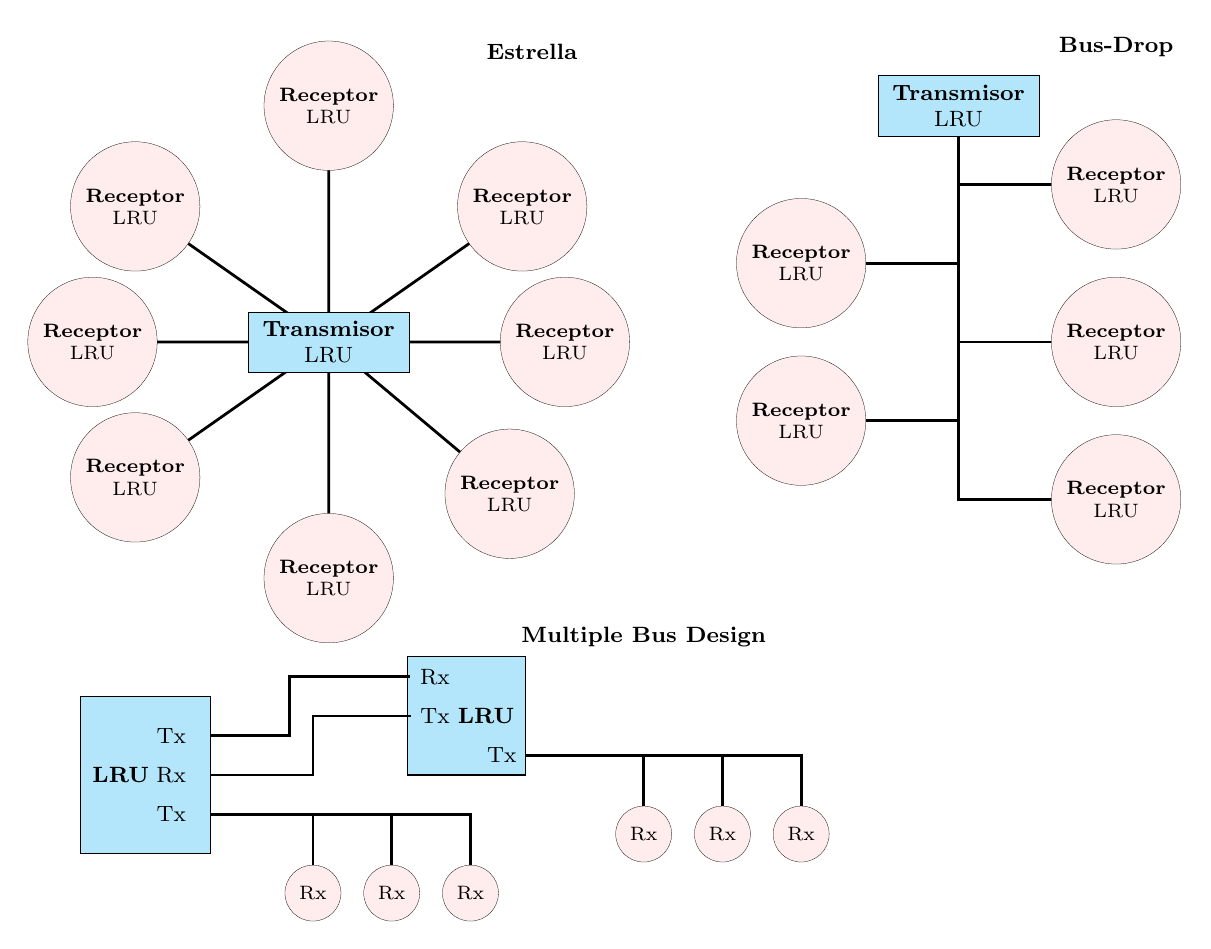
\begin{tikzpicture}[node distance=1cm, 
				font = \footnotesize , 
               Transmisor/.style ={ fill=cyan!30 , 
                          draw,
                          line width= 0.1 , 
						text width=1.8cm,
						align = center
                        } ,
               Receptor/.style ={  font = \scriptsize, 
						circle ,
                          fill=pink!30 , 
                          draw,
%						text width=1.2cm,
						align = center ,
                          line width= 0.1 , 
                        } ,
			]

% grilla
%  \draw[ green!50!black] (0,0) grid (20,10) ;

\path (3.5 , 7.5) coordinate (TxEstrella)
             (11.5 , 10.5) coordinate (TxBusDrop)
      ;

% Topologia estrella

\draw (TxEstrella) + (55:4.5) node {\bf Estrella};
\draw[line width=1]
               (TxEstrella) node[Transmisor]  {{\bf Transmisor} \\ LRU }
               -- +(0:3.0) node[Receptor]  {{\bf Receptor} \\ LRU }
(TxEstrella)  --  +(35:3.0) node[Receptor]  {{\bf Receptor} \\ LRU }
(TxEstrella)  --   +(90:3.0) node[Receptor]  {{\bf Receptor} \\ LRU }
(TxEstrella)  --   +(145:3.0) node[Receptor]  {{\bf Receptor} \\ LRU }
(TxEstrella)  --  +(180:3.0) node[Receptor]  {{\bf Receptor} \\ LRU }
(TxEstrella)  --   +(215:3.0) node[Receptor]  {{\bf Receptor} \\ LRU }
(TxEstrella)  --    +(270:3.0) node[Receptor]  {{\bf Receptor} \\ LRU }
(TxEstrella)  --    +(320:3.0) node[Receptor]  {{\bf Receptor} \\ LRU }
  ;

% Topologia estrella
\draw (TxBusDrop)  +(2,0.75)  node {\bf  Bus-Drop};
\draw[line width=1]
               (TxBusDrop) node[Transmisor]  {{\bf Transmisor} \\ LRU }
				         |- +(2,-1) node[Receptor]  {{\bf Receptor} \\ LRU }
(TxBusDrop) |- +(-2,-2) node[Receptor]  {{\bf Receptor} \\ LRU }
(TxBusDrop) |- +(2,-3) node[Receptor]  {{\bf Receptor} \\ LRU }
(TxBusDrop) |- +(-2,-4) node[Receptor]  {{\bf Receptor} \\ LRU }
(TxBusDrop) |- +(2,-5) node[Receptor]  {{\bf Receptor} \\ LRU }
;

% Topologia Multiple Bus Design

\draw [fill=cyan!30] (0.35,1) rectangle (2,3) 
	(1,2) node[text width=1cm] {\bf LRU}
		+ (0.5,0.5) node (Tx1) {Tx}
		+ (0.5,0.0) node (Rx1) {Rx}
		+ (0.5,-0.5) node (Tx11) {Tx}
;

\draw [fill=cyan!30] (4.5,2) rectangle (6,3.5) 
	(5.5,2.75) node {\bf LRU} +(2.0 , 1.0) node {\bf Multiple Bus Design}
		+ (-0.65,0.5) node (Rx2) {Rx}
		+ (-0.65,0.0) node (Tx2) {Tx}
		+ (0.2,-0.5) node (Tx22) {Tx}
;

\draw[line width=1] (Tx1) +(0.5 , 0) -- +(1.5,0) |- (Rx2) ;
\draw[line width=1] (Rx1) +(0.5 , 0) -- +(1.8,0) |- (Tx2) ;
\draw[line width=1] (Tx11) +(0.5 , 0) -- +(1.8,0) -- +(1.8 , - 1) node[Receptor] {Rx} ;
\draw[line width=1] (Tx11) +(0.5 , 0) -- +(2.8,0) -- +(2.8 , - 1) node[Receptor] {Rx} ;
\draw[line width=1] (Tx11) +(0.5 , 0) -- +(3.8,0) -- +(3.8 , - 1) node[Receptor] {Rx} ;

\draw[line width=1] (Tx22) +(0.3 , 0) -- +(1.8,0) -- +(1.8 , - 1) node[Receptor] {Rx} ;
\draw[line width=1] (Tx22) +(0.3 , 0) -- +(2.8,0) -- +(2.8 , - 1) node[Receptor] {Rx} ;
\draw[line width=1] (Tx22) +(0.3 , 0) -- +(3.8,0) -- +(3.8 , - 1) node[Receptor] {Rx} ;



\end{tikzpicture} 
%}
  \caption{Topologías ARINC 429, adaptado de \protect\cite{ARINC429Tutorial2010}}
  \label{fig:01.Topologias.ARINC429}
\end{figure}

Las  formas  de  conexión  más  utilizadas  para  conectar  las  LRU son la topología en Estrella o la Bus-Drop, Figura \ref{fig:01.Topologias.ARINC429}, donde cada LRU puede contener múltiples receptores y transmisores.

La mayor parte de la topología emplea una arquitectura punto a punto lo que proporciona alta fiabilidad en la transferencia de información.

\begin{myboxAzul}{Características del cableado}
  En este bus de
  comunicación se utiliza un par de cable trenzado y apantallado con
  una impedancia de 78$\Omega$.  El apantallamiento debe ir conectado
  a tierra al final de cada tramo y en cada unión de líneas.

La impedancia de salida del transmisor debe ser de $75 \Omega \pm 5 \Omega$
divididos equitativamente entre las líneas A y B, esta salida balanceada debe coincidir con la impedancia del cable. El receptor debe tener una impedancia efectiva de ingreso de $8\Omega$ como mínimo.

No se especifica una longitud máxima para los conductores, la mayoría de los sistemas emplean menos de 150 pies pero, si las condiciones lo permiten se puede llegar al doble de esta longitud o más.

\end{myboxAzul}
%\begin{myboxAzul}{Paquete de datos}

Como se indicó anteriormente el paquete de datos o palabra está formado por 
32 bits según la siguiente estructura:

\begin{center}
  \begin{tabular}[c]{c|c|c|c|c|c|c|c|c|c|c|c|c|c|c|c|c|c|} \cline{2-18}
    Bit & 32 & 31 & 30 & 29 & ......& 12 & 11 & 10 & 9 & 8 & 7 & 6 & 5 & 4 & 3 & 2 & 1 \\ \cline{2-18}
  Significado & {\bf P}
  & \multicolumn{2}{c|}{\bf SSM}
  & \multicolumn{4}{c|}{\bf Data} 
  & \multicolumn{2}{c|}{\bf SDI} 
  & \multicolumn{8}{c|}{\bf Label} 
\\ \cline{2-18}
  \end{tabular}
\end{center}



  \begin{itemize}
  \item Los 8 primeros bits son de etiqueta (Label), expresada en octal, identificando el tipo de datos.

El Label  se  expresa  como  3  dígitos codificados en octal por separado.
Se reservan los bits 1 y 2 para codificar el primer dígito del Label 
y los 6 restantes para codificar los dos últimos del Label.
Con esta estructura solo se puede codificar hasta 255 Labels.

% \begin{center}
%   \begin{tabular}[c]{c|c|c|c|c|c|c|c|c|} \cline{2-9}
%     Bit & 8 & 7 & 6 & 5 & 4 & 3 & 2 & 1 \\ \cline{2-9}
%   Dígito & \multicolumn{3}{|c|}{\bf Dígito 3}
%   & \multicolumn{3}{c|}{\bf Dígito 2}
%   & \multicolumn{2}{c|}{\bf Dígito 1} \\ \cline{2-9}
%   \end{tabular}
% \end{center}

  \item Los bits 9 y 10 corresponden al Source/Destination Identifier
    (SDI),  indican el origen y destino de los datos.
  \item Los bits comprendidos entre el 11 y el 29 son los datos
    (Data) que se encuentran codificados en sistema BCD o el BNR, que son las codificaciones comunes en ARINC 429. También se pueden utilizar formatos de datos mixtos.
    \begin{itemize}
    \item Binario (BNR)
    \item Decimal codificado en binario (BCD)
    \item Combinación de BNR y BCD
    \item Datos de mantenimiento
    \item Protocolo Williamsburg/Buckhorn
    \end{itemize}

  \item Los bits 30 y 31 corresponden al Sign/Status Matrix (SSM), indican si la palabra es válida. Los valores posibles son:
    \begin{description}
    \item[OP (operacional)] Indica que los datos de esta palabra se consideran correctos.
    \item[TEST]  Indica que los datos son proporcionados por una fuente de prueba.
    \item[FAIL]  Indica un error de hardware que ha causado pérdida de datos.

    \item[NCD] (no hay datos computados). Indica que faltan datos o que son inexactos, debido a alguna razón que no está vinculada al hardware. Por ejemplo, los comandos del piloto automático se muestran como NCD cuando el piloto automático no está activado.

    La SSM puede indicar también el signo (+/-) de los datos (por ejemplo usada en altura) o información relacionada, como la orientación (Norte / Sur / Este / Oeste).
  \end{description}
  
  \item El bit 32 es el de comprobación de paridad impar, se utiliza para
    verificar que la palabra no fue dañada durante la transmisión o
    que es ilegible.

%ParitybithelpstoDetectErrorinthereceivingwords.•ARINC429usesoddparityaserrorchecktoinsureaccuratedatareception.•ThenumberofLogic1stransmittedineachwordisanoddnumber.Thereceiverchecksthereceivedwordshavingoddlogicornot.•Oddlogic1s-accepttheword•Evenlogic1s-rejecttheword


\item De  todos  estos  campos  sólo  son obligatorios  dos:  el  bit  de  paridad  y  la etiqueta (Label).
  \end{itemize}

%\end{myboxAzul}


% \subsubsection{Cableado y topología}
% \label{sec:01.05.01.01.subsection.y.topologia}

% El protocolo 429 emplea una topología punto a punto muy simple en la que por
% cada cable solo puede existir un transmisor que siempre estará transmitiendo,
% ya sea palabras de 32 bits o el estado NULL, los receptores pueden ser desde
% 1, como mínimo, hasta 20. La transmisión por cada cable solo se realiza en un
% sentido.

% Este protocolo emplea transmisión unidireccional de palabras de 32 bits sobre
% dos pares trenzado usando formato bipolar RZ, en el bus conocido como Mark
% 33 \ac{DITS} a una tasa de envío de 12,5 o 100 kilobits por segundo.

% \subsubsection{Formato de trama}
% \label{sec:01.05.01.02.formato.de.trama}

% El formato de trama para este protocolo es el siguiente:

% \begin{table}[!h]
%   \centering

%   \caption{Trama para el ARINC 429}
%   \label{tab:formato.trama.ARINC.429}

%   \begin{tabular}{|c|c|c|cccccc|c|c|cc|} \hline
% 32 & 31 & 30 & 29 & & & & & 11 & 10 & 9 & 8 & 1 \\ \hline

% P & \multicolumn{2}{c|}{SSM} & DATA  $\Longrightarrow$ &\quad & $\Longleftarrow$ 
% & PAD & $\Longleftarrow$ & DISCRETES &
% \multicolumn{2}{c|}{SDI} & \multicolumn{2}{c|}{LABEL} \\ \hline 

%  & \multicolumn{2}{c|}{} & MSB  & & & & & LSB &
% \multicolumn{2}{c|}{} & \multicolumn{2}{c|}{ } \\ \hline 

    
%   \end{tabular}

% \end{table}


% Pasamos a explicar esta trama:

% \begin{itemize}

% \item \textbf{P} es el bit de paridad de la trama, suele estar fijado a impar
%   excepto para algunos tests, la paridad impar significa que hay un
%   numero de 1s impar. 

% \item {\bf \ac{SSM}}. Este
%   campo contiene el estado del hardware del equipo, el modo de
%   operación o la validez de los datos contenidos. Los valores que
%   pueden tomar aparecen en las siguientes tablas:
% \end{itemize}

% En esta tabla esta el significado de la pareja de bits en caso que sea
% información del tipo BCD, si la información fuera del tipo BCR deberíamos
% consultar la siguiente tabla.


% El campo Data engloba desde el bit 29 hasta el bit 11 de la trama, y como se
% puede esperar contiene los datos del protocolo. Estos datos pueden ser de
% diferentes formatos que pueden ser siguiendo los Standard o según el formato
% que el usuario quiera darle. Si necesitamos mas espacio este campo puede
% solaparse con el campo SDI, evidentemente en esos casos el campo SDI no se
% utiliza.

% \begin{itemize}
% \item El siguiente campo con el que nos encontramos es el SDI o
%   Source/Destination Identifier. Este es utilizado para cuando la
%   trama se envía a varios usuarios puedan saber a cual de ellos iba
%   realmente destinada la trama, a su vez puede ser destinado en caso
%   de sistemas múltiples para identificar el origen de la
%   transmisión. Recordemos que en 429 se puede tener un transmisor pero
%   hasta 20 receptores.

% \item El ultimo campo que tenemos es el Label o etiqueta, que nos
%   sirve para etiquetar el tipo de datos y los parámetros asociados a
%   el. Con este campo podemos deducir el método a usar para interpretar
%   los datos.  Reseñar el modo de transmisión de los datos ya que se
%   transmite a partir del bit 8 hasta el 1, es decir la etiqueta y
%   posteriormente se envía el resto de la trama a partir del bit 9
%   hasta el 32, quedaría de la siguiente forma:
% \end{itemize}

% 8, 7, 6, 5, 4, 3, 2, 1, 9, 10, 11, 12 ... 31, 32

% \subsubsection{Tipos de datos}
% \label{sec:tipos.de.datos}

% Anteriormente hemos hablado de los tipos de datos pero pasamos a explicarlos
% más detenidamente. Como hemos podido ver hasta ahora toda la información
% en 429 se transmite en palabras de 32 bits y puede estar en código decimal
% binario (BCD), complemento a dos binario (BNR), datos discretos, datos de
% mantenimiento y asentimiento, y por ultimo datos en caracteres ISO. Vamos a
% explicar cada uno de estos tipos de datos a continuación.

% Primero tenemos los datos BCD que son los más comunes en este protocolo y
% en otros protocolos similares. En este formato, 4 bits son asignados a cada
% carácter decimal, en este caso tendríamos espacio suficiente para 4 caracteres
% y un quinto que solo dispondría de 3 bits así que su valor máximo puede ser 7.
% Si necesitásemos que fuera mayor que 7 lo rellenamos con 0 y el segundo
% subcampo (bits del 26 al 23 según la numeración hecha anteriormente) seria el
% campo más importante desechando el primero.

% Los datos en un formato BNR también son muy comunes. Este tipo de
% codificación simplemente pone el número o dato como un número binario. El bit
% 29 es usado para el signo y el 28 es el bit más significativo (MSB) del campo de
% datos. Si el signo es negativo (bit 29 a ``1''), se trata de un numero negativo y
% esta codificado como complemento a dos de numero positivo. Para descifrar el
% valor de este campo suele ser necesario conocer la etiqueta asociada a la
% trama, explicaremos esto con un ejemplo a continuación.

% Sabiendo que la etiqueta es la 103 ya tenemos que la trama nos dirá la
% velocidad seleccionada. A partir del protocolo ya sabemos que la escala es 512
% y por lo tanto solo 11 bits se usan, desde el 29 al 19; como el bit 29 es 0
% sabemos que el número será positivo, el numero final lo deduciremos
% multiplicando por el factor de escala y después sumando todos los valores, el
% bit mas importante (bit 28) nos indica un factor de escala de 1/2, el siguiente nos
% indica 1/4 y así sucesivamente; como la escala en este caso es 512 tenemos
% que el valor seria 256 + 8 + 4 = 268 Knots, que es una medida de velocidad.

% También podríamos encontrar formatos mezclados entre estos dos tipos
% usando los bits que quedan inútiles.

% Otro formato a destacar son los formatos de datos discretos que son
% enumerados en la referencia 3 del protocolo. En ellos no tenemos un dato
% concreto sino que nos muestran el funcionamiento de distintos campos; como
% ejemplo podemos tomar la etiqueta 005 que nos da datos sobre el
% funcionamiento de del motor de transmisión.

% Por ultimo vamos a explicar el formato de datos de mantenimiento. Este
% formato se puede enviar tanto mensajes de mantenimiento como mensajes
% alfanuméricos, los alfanumérico suelen usar el alfabeto ISO No. 5. Este tipo de
% mensajes están controlados por un protocolo orientado a bit que será descrito
% posteriormente.

% Algunos ejemplos de las etiquetas se muestran a continuación en las dos
% siguientes tablas, en la primera es para el formato BCD y la segunda para el
% formato BNR.

% Destacar que los identificadores de los equipos nos dan mas información sobre
% la trama, por ejemplo en la tabla de BCD a pesar que la etiqueta 010 siempre
% indica latitud puede pertenecer a 3 orígenes distintos. Una misma etiqueta
% puede indicar datos distintos según cual sea su origen como podemos ver en la
% tabla de BCR. Para dejar esto mas claro ponemos a quien pertenecen los
% identificadores mostrados en las anteriores tablas

% \subsubsection{Modo de envío}
% \label{sec:01.05.01.04.modo.de.envio}

% Los mensajes en este protocolo suelen ser enviados varias veces, ya sea en
% secuencia de palabras o solo en tramas; por ejemplo podemos enviar una
% trama varias veces con un intervalo de 100 ms o pueden enviarse 5 tramas
% distintas en un intervalo y repetir esa secuencia varias veces.

% \subsubsection{Protocolo orientado a bit}
% \label{sec:01.05.01.06.protocolo.a.bit}


% Vamos a entrar mas detenidamente en el protocolo orientado a bit también
% conocido como el protocolo Williamsburg.

% Este protocolo se usa para enviar archivos entre unidades ARINCs. Los
% mensajes normales de ARINC 429 pueden ser mezclados con mensajes del
% tipo orientado a bit. Cuando un sistema quiere emplear este protocolo envía un
% mensaje usando la última versión que soporta, un proceso ajusta la versión
% hasta la más alta que soporten ambos.

% Para que inicie una transacción bajo este protocolo el código de inicio ha de ser
% ALO (de aloha) enviado a un potencial receptor, este mensaje ha de ser
% enviado justo cuando se inicie o cuando se reinicie por cualquier motivo. Si el
% receptor soporta este protocolo ha de enviar un ALR para que el transmisor
% sepa que puede seguir enviando bajo este protocolo, una vez ambos extremos
% han establecido la comunicación el origen envía un mensaje RTS (request to
% send) y espera a recibir un mensaje CTS (clear to send), el mensaje RTS
% incluye un código de destino y un contador de palabras que se repiten en el
% CTS para ser verificados. Los archivos son enviados en bloques conocidos
% como LDUs (Link Data Unit) que podría ser desde 3 hasta 255 palabras. La
% transmisión una vez permitida con el CTS se inicia con un SOT (Start Of
% Transmission) que incluye un número de secuencia, un identificador de formato
% general (GFI) y un número de secuencia de LDU. Al final de la secuencia se
% envía un EOT (End Of Transmission) que incluye un CRC, e identifica al LDU
% en una situación global en la transferencia del archivo; el receptor efectúa un
% control sobre el EOT y si todos los test se pasan envía una trama de
% aceptación ACK, y después el mismo destino envía otro CTS y el proceso se
% repite hasta que el ultimo LDU es confirmado. A continuación hacemos un
% esquema con la transacción de tramas en este protocolo:

% Algunos sistemas que usan este protocolo y su respectiva etiqueta puede ser
% vista en la siguiente tabla:

\subsubsection{Otros protocolos de la familia ARINC}
\label{sec:01.05.01.07.otros.protocolos.ARINC}


Hay otros protocolos del mismo estilo de ARINC 429 tales como:

\begin{description}

\item [ARINC  419] que fue sobre el que se basó el ARINC 429,  se trata de un protocolo
parecido en el que se incluyen palabras de 64 bits así como palabras de 32 bits.
Es bastante menos estandarizado para dar cabida a distintos
tipos de mensajes, tales como mensajes con etiquetas predeterminadas u otros
sin etiqueta alguna. %Es un protocolo mucho menos claro que el ARINC 429.

\item[ARINC 561] se basó en un sistema de seis hilos con tres pares  para DATA, SYNC y CLOCK. La codificación de no retorno a cero (NRZ) se empleó con la lógica 1 representada por 12 V. Al igual que ARINC 429, la longitud de la palabra fue de 32 bits con los bits 32 y 31 que comprenden la matriz de signo / estado (SSM) y no hay paridad disponible. Los campos incluyen una etiqueta de 8 bits y seis campos BCD, cinco de cuatro bits y uno de dos bits. Este sistema fue ampliamente utilizado en aviones fabricados antes de 1970. ARINC 568 usa la misma especificación de interfaz eléctrica que la utilizada en ARINC 561.

\item[ARINC 573] adoptado para su uso con Registradores de Datos de Vuelo (FDR, Flight Data Recorder) que utilizan un flujo continuo de datos de palabras codificadas de 12 bits de Harvard Bi-Phase. Estas palabras están codificadas en cuadros que contienen información instantánea de los datos de cada uno de los subsistemas de aviónica en el avión. Cada cuadro comprende cuatro subtramas. Una palabra de sincronización única aparece al comienzo de cada subtrama. ARINC 717 reemplaza a ARINC 573 y atiende a una serie de velocidades de bits y tamaños de trama diferentes.

\item[ARINC 575] similar al ARINC 429  es un sistema de bus de baja velocidad que se basa en un solo par de cables trenzados. Debido a la baja velocidad de datos admitida se considera obsoleto. Eléctricamente es generalmente compatible con ARINC 429 de baja velocidad. Sin embargo, algunas variantes de ARINC 575 usan una tasa de bits que es significativamente más lenta que ARINC 429 y pueden no ser compatibles en términos de especificaciones eléctricas y formatos de datos.

\item[ARINC 615] es un protocolo de software que se puede superponer sobre los sistemas compatibles con ARINC 429. Admite la transferencia de datos a alta velocidad hacia y desde los sistemas digitales integrados lo que permite, por ejemplo, leer y escribir discos de 3,5 pulgadas.

\item[ARINC 629] se introdujo a mediados de la década de 1990 y admite una velocidad de datos de 2 Mbps (20 veces más rápido que ARINC 429). El bus admite 120 dispositivos conectados y actualmente se utiliza en el Boeing 777, Airbus A330 y Airbus A340. Una mejora notable respecto de ARINC 429  es que  es un sistema de bus bidireccional por lo que los dispositivos conectados pueden transmitir, recibir o hacer ambas cosas. También  logra la comunicación bidireccional del bus sin la necesidad de un controlador de bus. El medio del bus físico es un par trenzado blindado (STP).

\item[ARINC 708] se utiliza para transferir datos desde el receptor de radar meteorológico en el aire a la pantalla de radar de la aeronave. El bus es unidireccional y utiliza datos codificados en Manchester a una velocidad de 1 Mbps. Las palabras de datos tienen una longitud de 1600 bits:
  \begin{itemize}
      \item una palabra de estado de 64 bits y
      \item 512 palabras de datos de 3 bits
  \end{itemize}

\end{description}

\subsubsection{Avionics Full-Duplex Switched Ethernet (AFDX)}
\label{sec:01.05.AFDX}

Basado en ARINC 664 Parte 7 contribuye al modelo IMA (Integrated Modular Avionics) que presenta nuevas topologías de arquitectura y nuevas amenazas de seguridad.
 
 El Airbus A380 fue el primer avión en utilizar el bus de aviónica basado en el protocolo AFDX. 




\subsubsection{MIL-STD-1553}
\label{sec:01.02.MIL.STD.1553}

Es un protocolo de carácter militar del Departamento de Defensa de  EEUU. 
Ha encontrado su uso, preferente, en aeronaves o helicópteros militares, además
es la interfaz preferida entre la nave y los misiles. 
También se lo puede encontrar este protocolo en barcos, submarinos, tanques de combate y naves espaciales.

Este protocolo especifica las características mecánicas, eléctricas y operativas de un bus de transmisión de datos en serie. 

 MIL-STD-1553 es la contraparte militar de ARINC-429 y posee diferencias estructurales puesto que, en las
aeronaves militares, se exige que el diseño permita seguir controlando la misma en caso de corte de un cable o  el  mazo de los mismos.

En 1978 apareción  MIL-STD-1553B que reemplazó a la anterior  MIL-STD-1553A de 1975. 
%La diferencia fundamental entre estas revisiones es que las opciones se especifican en la última en lugar de dejar que el consumidor las identifique según sea necesario. 
%Es responsabilidad de la SAE (Society of American Engineers) proporcionar reparaciones y cualquier mejora potencial a la norma. 
La mayoría de los sistemas modernos emplean el formato MIL-STB1553B.
La última revisión es MIL-STD-1553C realizada en febrero de 2018. 


Como características principales se tienen:

\begin{itemize}
\item Velocidad de envío de datos de 1Mb/seg
\item Tamaño de palabras de 16 bit
\item Comunicación half-duplex asíncrona.
\item Posee la técnica TDM (Time Division Multiplex) en la cual la transmisión se realiza bajo petición.
\item Sistema de codificación Manchester II bifase.
\item Hasta 31 terminales conectadas al mismo bus.
\item Tres tipos de terminales:
  \begin{itemize}
  \item Bus Monitor (BM)
  \item el Bus Controller (BC)
  \item y los terminales remotos, o Remote Terminals (RT)
  \end{itemize}
\end{itemize}

\begin{figure}[!h]
  \centering
%  \scalebox{0.9}{
% MIL-STD-1553
% esquema del bus
% version 2021

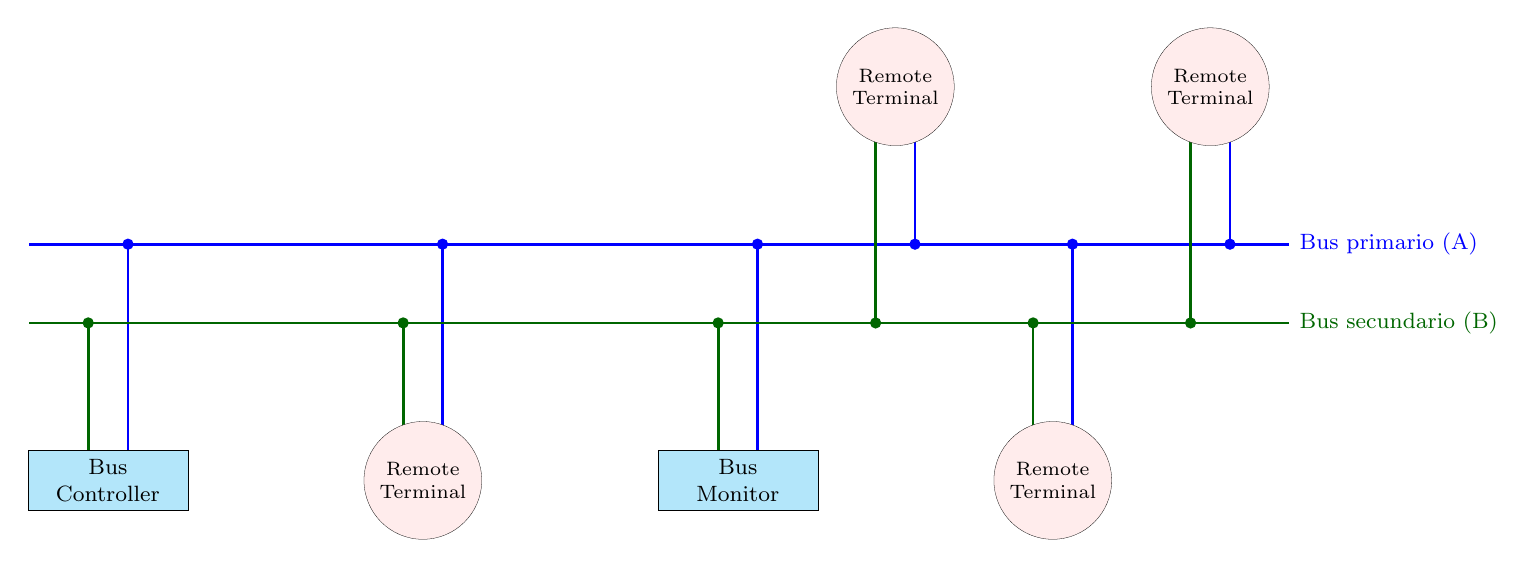
\begin{tikzpicture}[ node distance=1cm,
             conexion/.style = { circle, 
                                                 minimum size = 3 ,
                                              draw,
												fill ,
											inner sep=0 ,
                                                },
				font = \footnotesize , 
               Transmisor/.style ={ fill=cyan!30 , 
                          draw,
                          line width= 0.1 , 
						text width=1.8cm,
						align = center
                        } ,
               Receptor/.style ={  font = \scriptsize, 
						circle ,
                          fill=pink!30 , 
                          draw,
%						text width=1.2cm,
						align = center ,
                          line width= 0.1 , 
                        } ,
                     ]

% grilla
%  \draw[ green!50!black] (0,0) grid (20,10) ;

% Bus primario
\draw[line width=1, blue]  (0 , 4) -- +(16 , 0) node[above, right] {Bus primario (A)}
                       (1.255 , 4 ) node[conexion ] {} -- +(0 , -3) 
                       (5.25 , 4 ) node[conexion ] {} -- +(0 , -3) 
                       (9.25 , 4 ) node[conexion ] {} -- +(0 , -3)
                        (11.25 , 4 ) node[conexion ] {} -- +(0 , 2)
                       (13.25 , 4 ) node[conexion ] {} -- +(0 , -3) 
                       (15.25 , 4 ) node[conexion ] {} -- +(0 , 2) 
;

% Bus secundario
\draw[line width=1, green!40!black]  (0 , 3) -- +(16 , 0) node[above, right] {Bus secundario (B)} 
                       (0.75 , 3 ) node[conexion ] {} -- +(0 , -2) 
                       (4.75 , 3 ) node[conexion ] {} -- +(0 , -2) 
                       (8.75 , 3 ) node[conexion ] {} -- +(0 , -2) 
                      (10.75 , 3 ) node[conexion ] {} -- +(0 ,  3)
                      (12.75 , 3 ) node[conexion ] {} -- +(0 ,  -2)
                      (14.75 , 3 ) node[conexion ] {} -- +(0 ,  3)
;

% Elementos del bus
\draw ( 1 ,1 ) node[Transmisor] (BS) {Bus \\Controller} 
            +( 4 , 0 ) node[Receptor] (RT1) {Remote \\Terminal} 
            +( 8 , 0 ) node[Transmisor] (BM) {Bus \\ Monitor} 
            +( 10 , 5 ) node[Receptor] (RT2) {Remote \\Terminal} 
            +( 12 , 0 ) node[Receptor] (RT3) {Remote \\Terminal} 
            +( 14 , 5 ) node[Receptor] (RT4) {Remote \\Terminal} 
;





\end{tikzpicture}
%}
  \caption{Arquitectura de MIL-STD-1553, adaptado de \protect\cite{MIL-1553-tutorial}}
  \label{fig:01.MIL.1553.componentes}
\end{figure}



\subsubsection{STANAG 3838}
\label{sec:01.02.STANAG.3838}

\begin{myboxAmarillo}{STANAG}
  El STANdardization AGreement (STANAG, Acuerdo de Normalización) de
  la OTAN (Organización del Tratado del Atlántico Norte) definen
  procesos, procedimientos, términos y condiciones de equipamiento o
  procedimientos y técnicas militares comunes entre los países
  miembros de dicha alianza.
\end{myboxAmarillo}


El protocolo MIL-STD-1553 
fué adoptado por la OTAN como STANAG 3838 empleando el método de transmisión bidireccional por una sola línea  de 16 bits. Es redundante porque emplea dos buses y dos controladores de bus. Su velocidad de transmisión es de 1Mb/seg.

\subsubsection{STANAG 3910 }
\label{sec:01.02.STANAG3910 }

Es un protocolo de bus de alta velocidad de 16 bit bajo STANAG 3838 o control equivalente mediante fibra óptica. Se emplea principalmente para uso en sistemas de aviónica y que permite aumentar un bus de datos STANAG 3838 o MIL-STD-1553B de 1 Mb/seg a un bus de datos de alta velocidad de 20 Mb/seg denominado canal HS mediante, entre otros elementos, el uso de fibra óptica..

El bus STANAG 3838 / MIL-STD-1553B en una implementación de STANAG 3910 se denomina canal de baja velocidad (LS) y emplea canales de cobre. 

Ambos canales o cualquiera de ellos pueden tener redundancia múltiple y emplear medios eléctricos u ópticos.

\subsubsection{CSDB y ASCB}
\label{sec:01.02.CSDB+ASCB}

Son protocolos patentados de Collins (CSDB) y Honeywell (ASCB). 
Estos sistemas se utilizan a menudo en pequeñas empresas y aviones privados de aviación general. 

CSDB es un bus unidireccional que permite la conexión de hasta diez receptores y un transmisor. El estándar admite velocidades de datos de 12,5 kbps y 50 kbps. 

ASCB es un bus bidireccional controlado centralmente. Una configuración básica comprende un controlador de bus único y dos buses aislados, cada uno de los cuales puede admitir hasta 48 dispositivos.

\subsubsection{FDDI}
\label{sec:01.02.FDDI}

La Interfaz de Datos Distribuidos por Fibra (FDDI) fue desarrollada originalmente por Boeing para su uso en el avión Boeing 777. 

FDDI es una red de área local (LAN) basada en una topología de anillo de token dual. Los datos en cada anillo fluyen en direcciones opuestas. La velocidad de datos es de 100 Mbps y los datos se codifican en cuadros. 
CDDI (Interfaz de Datos Distribuidos de Cobre) y SDDI (Interfaz de Datos Distribuidos de Par Trenzado Blindado) son estándares de bus de red similares empleando como medios físicos cables de cobre y par trenzado blindado. 
El formato de datos es NRZI, formato de datos similar a NRZ, pero en el cual un cambio en el nivel de voltaje de línea indica un 1 lógico y ningún cambio indica un 0 lógico. 
%Por razones de costo y para reducir el número y la complejidad de los estándares de red utilizados en sus aeronaves avión, Boeing ahora planea reemplazar el sistema en el 777 con un ethernet de cobre de 10 Mbps menos costoso.


% Versión 2021
%

% Capítulo 2. Medición de datos de aire
% 2.1.  Circuitos de presiones estática y total. Toma de presiones alternativas
% 2.2.  Altímetros barométricos, servoaltímetros. Codificadores de altura
% 2.3.  Variómetros
% 2.4.  Velocímetros. Machmetros.
% 2.5.  Computadores centrales de datos de aire, su función

% \section{Introducci\'on}
% \label{sec:U02.00.introduccion}


 \chapter{Medici\'on de datos de aire}
 \label{chap:U02.medicion.datos.aire}


\begin{flushright}
  Por el Prof. Ing. Ángel Galeasso
\end{flushright}

% \section{Circuitos de presiones estática y total. Toma de presiones alternativas}
% \label{sec:U02.01.circuitos.p.estat.y.total.tomas.presiones.alternativas}


% \section{Altímetros barométricos, servoaltímetros. Codificadores de altura}
% \label{sec:U02.02.altimetros.codificadores.altura}


% \section{Variómetros}
% \label{sec:U02.03.variometros}


% \section{Velocímetros. Machmetros}
% \label{sec:U02.04.Velocimetros.Machimetros}


% \section{Computadores centrales de datos de aire, su función}
% \label{sec:U02.05.computadores.datos.aire}

\begin{landscape}

  \includepdf[pages=-, fitpaper=false, scale=0.80, landscape=true,
  offset = 0 -20,
  pagecommand={\thispagestyle{fancy}}]
  {02.medicion.datos.aire/instrumentos-2019.pdf}

\end{landscape}


% Versión 2021
%

% Capítulo 3. Instrumentos de motores
% 3.1.      Taquímetros mecánicos , eléctricos, electrónicos.
% 3.2.      Flujómetros, diferentes tipos, totalizadores.
% 3.3.      Indicadores de empuje, indicadores de torque.
% 3.4.      Termocuplas. Medición de la temperatura en motores.

\chapter{Instrumentos de motores}
\label{chap:U03.instrumentos.de.motores}




\section{Introducci\'on}
\label{sec:U03.00.introduccion}

\begin{flushright}
  Por el Prof. Ing. Pedro Giraudo
\end{flushright}

\section{Taquímetros mecánicos , eléctricos, electrónicos}
\label{sec:U03.01.taquimetros}

  \includepdf[pages=-, fitpaper=false, scale=1.0, %landscape=true,
  offset = 0 -20,
  pagecommand={\thispagestyle{fancy}}]
{03.instrumentos.motores/Taquimetros.pdf}

\section{Flujómetros, diferentes tipos, totalizadores}
\label{sec:U03.02.flujometros}

  \includepdf[pages=-, fitpaper=false, scale=1.0, %landscape=true,
  offset = 0 -20,
  pagecommand={\thispagestyle{fancy}}]
{03.instrumentos.motores/MedicionDelFlujoDeCombustible.pdf}

% \section{Indicadores de empuje, indicadores de torque}
% \label{sec:U03.03.indicadores.empuje}

\section{Termocuplas. Medición de la temperatura en motores}
\label{sec:U03.termocuplas}


  \includepdf[pages=-, fitpaper=false, scale=1.0, %landscape=true,
  offset = 0 -20,
  pagecommand={\thispagestyle{fancy}}]
{03.instrumentos.motores/MedicionDeTemperaturaEnMotoresTermometrosTermoelectricos.pdf}

%  Versión 2021
%

% Capítulo 4. Instrumentos de control
% 4.1.      Indicación de la cantidad de combustible, eléctrica y electrónica
% 4.2.      Indicadores de posición a distancia de CC y CA.
% 4.3.      Termómetros, diferentes tipos de lectura directa y a distancia
% 4.4.      Medidores de presión, diferentes tipos de lectura directa y a distancia.

\chapter{Instrumentos de Control}
\label{chap:U04.instrumentos.ctrol}

% \section{Introduccion}
% \label{sec:U04.00.introduccion}


% \section{Indicación de la cantidad de combustible, eléctrica y electrónica}
% \label{sec:U04.01.indicacion.cantidad.combustible}


\section{Indicadores de posición a distancia de CC y CA}
\label{sec:U04.02.indicadores.posicion.a.distancia.cc.ca}

\begin{flushright}
  Por el Prof. Ing. Pedro Giraudo
\end{flushright}



  \includepdf[pages=-, fitpaper=false, scale=1.0, %landscape=true,
  offset = 0 -20,
  pagecommand={\thispagestyle{fancy}}]
{04.instrumentos.ctrol/SistemasSincronosDeTransmisionDeDatos.pdf}

% \section{Termómetros, diferentes tipos de lectura directa y a distancia}
% \label{sec:U04.03.termometros}


% \section{Medidores de presión, diferentes tipos de lectura directa y a distancia}
% \label{sec:U04.04.medidores.presion}



% Versión 2021
%


% Capítulo 5. Instrumentos giroscópicos
% 5.1.       Propiedades giroscópicas aplicadas al instrumental aeronáutico de a bordo.
% 5.2.       Indicadores de virajes, neumáticos, de CC y CA .
% 5.3.       Indicadores de actitud en dos ejes con giróscopo integrado, y remoto.
% 5.4.       Magnetismo terrestre, brújula, giróscopo direccional libre.
% 5.5.       Compás giroscópico auto-corregido, indicador con giróscopo integrado, y remoto.
% 5.6.       Central giroscópica para la indicación de actitud en tres ejes y toda actitud.
% 5.7.       Giróscopo LASER


\chapter{Instrumentos girosc\'opicos}
\label{sec:instrumentos.giroscopicos}

\begin{flushright}
  Por el Prof. Ing. Ángel Galeasso
\end{flushright}


\begin{landscape}

  \includepdf[pages=-, %fitpaper=true,
  scale=0.80, landscape= true, offset = 0 -20,
  pagecommand={\thispagestyle{fancy}}]
  {05.instrumentos.giroscopicos/instrumentos_giroscopicos_Galeasso/01_instrumentos_2020_GIROSCOPOS.pdf}

  \includepdf[pages=-33, %fitpaper=true,
  scale=1, landscape= true, offset = 0 -20,
  pagecommand={\thispagestyle{fancy}}]
  {05.instrumentos.giroscopicos/instrumentos_giroscopicos_Galeasso/03_Principios_basicos_del_giroscopio.pdf}

  \includepdf[pages=-, %fitpaper=true,
  scale=0.9, landscape= true, offset = 0 -20,
  pagecommand={\thispagestyle{fancy}}]
  {05.instrumentos.giroscopicos/instrumentos_giroscopicos_Galeasso/04_Indicador_de_viraje_2020.pdf}

\end{landscape}

  \includepdf[pages=-, %fitpaper=true,
  scale=0.9, landscape= false, offset = 0 -20,
  pagecommand={\thispagestyle{fancy}}]
  {05.instrumentos.giroscopicos/instrumentos_giroscopicos_Galeasso/05_Horizonte_artificial.pdf}

  \begin{landscape}

  \includepdf[pages=-, %fitpaper=true,
  scale=0.8, landscape= true, offset = 0 -20,
  pagecommand={\thispagestyle{fancy}}]
  {05.instrumentos.giroscopicos/instrumentos_giroscopicos_Galeasso/06_Magnetismo_terrestre.pdf}

  \includepdf[pages=-, %fitpaper=true,
  scale=0.9, landscape= true, offset = 0 -20,
  pagecommand={\thispagestyle{fancy}}]
  {05.instrumentos.giroscopicos/instrumentos_giroscopicos_Galeasso/07_Giroscopo_direccional.pdf}
    
  \end{landscape}


\subsection{Videos sobre instrumentos girosc\'opicos}
\label{sec:05.videos.instrumentos.giroscopicos}

  \begin{itemize}

  \item PARTE 1--                                                                     

    \begin{itemize}
    \item \href{https://www.youtube.com/watch?v=fVefWA-SV2g&feature=relmfu}{Giróscopo
        educativo }

    \item \href{https://www.youtube.com/watch?v=VXePbCxCzRA}{Giróscopo
        educativo }

    \item \href{https://www.youtube.com/watch?v=-NSUIEOPjrY}{Analogía
        traslación-rotación}
    \end{itemize}

  \item PARTE 3--

\href{https://www.youtube.com/watch?v=hVsx4XWafXg}{Video  general sobre giróscopo }

\item PARTE 4—Indicador de viraje

  \begin{itemize}
  \item \href{https://www.youtube.com/watch?v=0sRrSkSJc7w}{Indicador
      de viraje }

  \item \href{https://www.youtube.com/watch?v=a4iLtZPp_-8}{Indicador
      de viraje }
  \end{itemize}


\item PARTE 5-- Horizonte artificial

  \begin{itemize}
  \item \href{https://www.youtube.com/watch?v=f2thngd9AGI}{Horizonte
      artificial neumático}

  \item
    \href{https://www.facebook.com/1Elaviador/videos/492439044662271/}{Horizonte
      artificial }

  \item
    \href{https://www.facebook.com/Pilotviewglobal/videos/354425058384879/}{Horizonte
      artificial }

  \item \href{https://www.youtube.com/watch?v=VycrS3VYjeM}{Horizonte
      artificial}
  \end{itemize}

\item PARTE 6-- Magnetismo terrestre

\href {https://www.youtube.com/watch?v=4dDKjdj_Dvc}{Brújula magn\'etica}

% \item PARTE 7-- Compás giroscópico

% \item PARTE 8—Bases inerciales

% https://www.youtube.com/watch?v=pvRsA-bk4b4       MIG 21

% https://www.youtube.com/watch?v=LaxsIgxnf_E          MIG 23

% https://www.youtube.com/watch?v=U2JvtNbGVZc        F-104 Starfighter

\item PARTE 9--Giróscopo laser

  \begin{itemize}
  \item \href{https://www.youtube.com/watch?v=ox-LRneg1VY}{Giróscopo
      laser}

  \item \href{https://www.youtube.com/watch?v=Fk0RvzaHq_Q}{Efecto
      Sagnac}
  \end{itemize}

\end{itemize}

% \section{Introducci\'on}
% \label{sec:U05.00.introduccion}


% \section{Propiedades giroscópicas aplicadas al instrumental aeronáutico de a bordo}
% \label{sec:U05.01.propiedades.giroscopicas}


% \section{Indicadores de virajes, neumáticos, de CC y CA}
% \label{sec:U05.02.indicadores.virajes}


% \section{Indicadores de actitud en dos ejes con giróscopo integrado, y remoto}
% \label{sec:U05.03.indicadores.actitud.en.dos.ejes}

% \section{Magnetismo terrestre, brújula, giróscopo direccional libre}
% \label{sec:U05.04.magnetismo.terrestre}


% \section{Compás giroscópico auto-corregido, indicador con giróscopo integrado, y remoto}
% \label{sec:U05.05.instrumentos.giroscopicos}


% \section{Central giroscópica para la indicación de actitud en tres ejes y toda actitud}
% \label{sec:U05.06.central.giroscopica}


% \section{Giróscopo LASER}
% \label{sec:U06.07.giroscopo.laser}



% Version 2023
%

% Capítulo 6. Radionavegación
% 6.1      ADF, función, diagrama en bloque, principio de funcionamiento.
% 6.2      VOR, función, diagrama en bloque, principio de funcionamiento.
% 6.3      ILS, función, diagrama en bloque, principio de funcionamiento.
% 6.4      DME, función, diagrama en bloque, principio de funcionamiento.
% 6.5      Radio-altímetro
% 6.6      Radar meteorológico.                                            

\chapter{Radionavegaci\'on}
\label{chap:U06.radionavegacion.tex}


\section{M\'etodos de Navegaci\'on A\'erea}
\label{sec:06.metodos.navegacion.aerea}

La navegaci\'on a\'erea se divide en dos tipos, dependiendo de si la aeronave es independiente o necesita de instalaciones exteriores a la aeronave para poder guiarse:

\CajaAmarilla{Navegaci\'on A\'erea Aut\'onoma}{	
Es aquella que no necesita de alguna infraestructura o informaci\'on suministrada 
	por un equipo exterior a la aeronave para poder completar con \'exito el vuelo. 
	A su vez, \'esta se divide en:

\begin{description}

    \item [Navegaci\'on observada:] se basa en la observaci\'on directa por parte del navegante o piloto de las referencias necesarias en el terreno para conocer la posici\'on de la aeronave.

    \item [Navegaci\'on a estima (Dead reckoning):] el navegante o piloto estima la posici\'on actual, conocidas la direcci\'on y la velocidad respecto al terreno.

    \item [Navegaci\'on por fijaci\'on de la posici\'on:] \'esta a su vez se subdivide en navegaci\'on a\'erea astron\'omica, navegaci\'on a\'erea Doppler, \ac{INS}.

\end{description}

}

\CajaAmarilla{Navegaci\'on A\'erea No Aut\'onoma}{
 Necesita de instalaciones exteriores para su guiado durante el vuelo, estas reciben el nombre de \emph{ayudas a la navegaci\'on}, las cuales se pueden dividir a su vez dependiendo del tipo de informaci\'on que transmiten as\'i como del canal a trav\'es del cual lo hacen. 
De esta manera las ayudas pueden ser:

\begin{description}
    \item [Ayudas visuales al aterrizaje:] son instalaciones que proporcionan se\~nales visuales durante la etapa de aterrizaje de la aeronave.

    \item [Radioayudas:] Se basan en se\~nales radioel\'ectricas, usualmente generadas en instalaciones terrestres y recibidas a bordo.

    \item [Navegaci\'on por sat\'elite:] se basa en una constelaci\'on de sat\'elites que transmite rangos de se\~nales utilizados para el posicionamiento y localizaci\'on en cualquier parte del globo terrestre, ya sea en tierra, mar o aire. Estos permiten determinar las coordenadas geogr\'aficas y la altitud de un punto dado como resultado de la recepci\'on de se\~nales provenientes de dicha constelaci\'on.

\end{description}
}

\begin{figure}[!h]
  \centering
  \includegraphics[width=0.7\textwidth]{06.radionavegacion/Imagenes/tipos-navegacion.eps}
  \caption{Navegaci\'on A\'erea}
  \label{fig:navegacion.aerea.cuadro}
\end{figure}

\section{Radionavegaci\'on}
\label{sec:06.radionavegacion.principios}

Se suele denominar como Radionavegaci\'on a las t\'ecnicas y sistemas que permiten estimar la posici\'on de un veh\'iculo, ya sea terrestre, naval o a\'ereo, empleando se\~nales de radio.

Estos sistemas empezaron a desarrollarse a principios del siglo XX junto con el desarrollo de la radio y, al día de hoy, se contin\'uan desarrollando por la gran multitud de aplicaciones que éstos tienen.

Los sistemas de radionavegación emplean estaciones, o radiayudas, para enviar o recibir señales. Seg\'un  donde se encuentren dispuestas estas estaciones pueden clasificarse los sistemas de radionavegación como terrestres, si se usan estaciones terrestres, y sistemas de radionavegación por satélite, si se emplean constelaciones de satélites en la \'orbita terrestre.

Todos estos sistemas basan su funcionamiento en las ondas de radio.
 Por ello, es conveniente comenzar con los conceptos b\'asicos asociados a las ondas en general y a las ondas electromagn\'eticas en particular, de las cuales las ondas de radio son apenas un subconjunto.

\subsection{ Ondas Electromagn\'eticas }
\label{sec:06.ondas.electromagneticas}


\subsubsection{Caracter\'isticas generales}
\label{sec:06.ondas.electromagneticas.caracteristicas.generales}

Una onda electromagn\'etica es un tipo de radiaci\'on en forma de onda que se caracteriza por poseer dos campos: un campo el\'ectrico ($\vec{E}$) y otro campo magn\'etico ($\vec{B}$), oscilando perpendicularente entre s\'i. La Figura \ref{fig:onda-electromagnetica} representa una onda electromagn\'etica: 

\begin{figure}[!h]
  \centering
  \includegraphics[width=0.5\textwidth]{06.radionavegacion/Imagenes/06.00.ondas.electromagneticas/onda_electromagnetica.jpg}  
  \caption{Onda electromagn\'etica \protect\cite{onda_electro_magnetica}}
  \label{fig:onda-electromagnetica}
\end{figure}



% Dibujar en Tikz onda electromagnética ver:

% \url{https://tex.stackexchange.com/questions/229674/electromagnetic-wave-propagation-with-tikz}


% Link que explica de forma simple y con dibujos: 
% \url{https://ikastaroak.ulhi.net/edu/es/IEA/ICTV/ICTV02/es_IEA_ICTV02_Contenidos/website_index.html}



Para entender mejor su comportamiento se recuerdan los siguientes conceptos:

\begin{description}
\item [Ciclo] Es cada patr\'on repetitivo de una onda.

\item  [Per\'iodo] Tiempo que tarda la onda en completar un ciclo, se lo suele denominar $T$.

\item  [Frecuencia] N\'umero de ciclos que completa la onda en un intervalo de
  tiempo. Se la suele designar $f$.
  Si dicho intervalo es de un segundo, la unidad de frecuencia
  es el Hertz (Hz). Otras unidades de frecuencias muy utilizadas (en
  otros \'ambitos) son las ``\textit{revoluciones por minuto}'' (RPM) y los
  ``\textit{radianes por segundo}'' (rad/s).

El per\'iodo y la frecuencia est\'an relacionados mediante la expresión: $ f = 1/T $

\item [Amplitud] Es la medida de la magnitud de la m\'axima perturbaci\'on del medio producida por la onda.

\item [Longitud de onda] Determinada por la distancia entre los puntos inicial y final de un ciclo (por ejemplo, entre un valle de la onda y el siguiente). Habitualmente se denota con la letra griega $\lambda$ (lambda).
En la Figura
donde se mantiene el tiempo $t$ constante y la distancia $x$ variable 


En el caso de las ondas electro magn\'eticas 
la amplitud del campo el\'ectrico o del magn\'etico se puede expresar como:

\[ E = E_0 \,\cos{(     \omega \,t + \varphi)}
\]

Donde $E_0$ es la amplitud m\'axima, en este caso del campo el\'ectrico,  considerando el eje $x$
como direcci\'on de propagaci\'on, 
%$k$ es el n\'umero de onda, 
$\varphi$ es la fase inicial
de la onda y $\omega$ la frecuencia angular.
% Estos valores se relacionan entre s\'i de la siguiente manera:

% \[ \displaystyle k = \frac{2\pi}{\lambda} \quad [\text{radianes/m}] 
%    \qquad \omega = 2\pi\,f \quad [\text{radianes/seg}]
% \]

% Donde $\lambda$ es la longitud de onda en metros y $f$ es la frecuencia de la misma en Hertz.


Un factor importante a tener en cuenta es que el tama\~no y dise\~no de las antenas est\'a fuertemente influenciado por la longitud de onda. Por ejemplo, una antena dipolo sencilla debe tener una longitud $\lambda/2$ para que sintonice de manera \'optima las ondas de longitud $\lambda$.

Los conceptos anteriores est\'an representados en la Figura \ref{fig:propiedades-onda}.

\begin{figure}[!h]
  \centering
 \includegraphics[width=0.7\textwidth]{06.radionavegacion/Imagenes/06.01.adf/propiedades-onda.png}  
  \caption{Propiedades de una onda \protect\cite{wikipedia_esp}}
  \label{fig:propiedades-onda}
\end{figure}


\item [Velocidad] Las ondas se desplazan a una velocidad que depende de la naturaleza de la onda y del medio por el cual se mueven. En el caso de la luz, por ejemplo, la velocidad en el vac\'io se denota $c$ y vale 299792458 m/s (aproximadamente $3 \times 10^8 \, m/s$).

Los conceptos de velocidad, longitud y frecuencia est\'an interrelacionados. Para el caso de las ondas electromagn\'eticas (de las cuales la luz es un ejemplo), la relaci\'on se expresa como $ \lambda = c / f $

\begin{tcolorbox}
  \begin{sagesilent}
# Ejemplos sobre ondas electromagneticas
# 22/09/2020  SageMath 


long_onda_01 = 30           # [m] longitud onda dato
velocidad_luz = 3 * 10**8   # [m/seg] velocidad de la luz en vacio

frecuencia_01 = velocidad_luz / long_onda_01  # [Hz] frecuencia correspondiente a long_onda_01

frecuencia_02 = 300         # [MHz] frecuencia dato
long_onda_02  = velocidad_luz / frecuencia_02 / 10**6 # [m] long_onda correspondiente a frecuencia_02

  \end{sagesilent}

{\bf Ejemplos:}

  \begin{itemize}
  \item Si se tiene onda electromagn\'etica con $\lambda_1 =
    30$ \,m, ¿ cu\'al es la frecuencia
    asociada?

    Recordando la expresi\'on anterior, se hace:

    \[ \text{frecuencia}_1 = \displaystyle \frac{c}{\lambda_1} =
    \displaystyle
    \frac{ 3\times10^8 \text{\,m/seg}}{ 30 \text{\,m}}
    =  10000000 \,\text{Hz} =
    10,\text{MHz}
    \]

  \item Si se tiene onda electromagn\'etica con frecuencia$_2 =
    300$\,MHz, ¿ cu\'al es la longitud de onda 
    asociada?

    Recordando la expresi\'on que relaciona estos valores, se hace:

\[ \displaystyle 
	\lambda_2 = \frac{c}{\text{frecuencia\,}_2} 
	= \frac{3\times10^8 \text{\,m/seg}}{ 300 \text{\,MHz}}
	= \frac{3\times10^8  \text{\,m/seg}}{ 300000000 \text{\,Hz}}
	=  1  \text{\,m}
\]

  \end{itemize}

\end{tcolorbox}


\item [Fase] La fase de una onda relaciona la posici\'on de una caracter\'istica espec\'ifica del ciclo (como por ejemplo un pico), con la posici\'on de esa misma caracter\'istica en otra onda. Puede medirse en unidades de tiempo, distancia, fracci\'on de la longitud de onda o (m\'as com\'unmente) como un \'angulo.

Tomese en cuenta que la definici\'on de fase lleva impl\'icita la comparaci\'on de dos ondas de la misma frecuencia, pues en caso contrario no tiene mucho sentido dicha comparaci\'on.

La Figura \ref{fig:desfase-ondas} muestra varias ondas con diferentes fases. 

\begin{figure}[!h]
  \centering
  \includegraphics[width=0.7\textwidth]{06.radionavegacion/Imagenes/06.01.adf/desfase-ondas.png}
  \caption{Ondas con diferentes fases \protect\cite{wikipedia_esp}}
  \label{fig:desfase-ondas}
\end{figure}


\item [Polarizaci\'on] Representa la orientaci\'on con la que la onda oscila y, en el caso particular de las ondas electromagn\'eticas, la orientaci\'on en la oscilaci\'on del campo el\'ectrico. 
Pueden ser del siguiente tipo:

\begin{description}
\item[\bf Polarizaci\'on Plana o Lineal:] A menudo esta orientaci\'on es una l\'inea y por ello se habla t\'ipicamente de ondas con polarizaci\'on vertical u horizontal, es decir, cuando el campo el\'ectrico oscila en un plano con esas direcciones.
  \begin{description}
  \item[\bf Polarizaci\'on Horizontal:] Si el campo eléctrico se propaga en dirección paralela a la superficie de la tierra.
  \item[\bf Polarizaci\'on Vertical:] Si el campo eléctrico se propaga perpendicularmente a la superficie terrestre.
  \end{description}

\item[\bf Polarizaci\'on Circular:] Cuando el campo el\'ectrico cambie su orientaci\'on conforme la onda avanza, girando 360º a medida de que la onda recorre una distancia $\lambda$ y la intensidad de $\vec{E}$ es igual en todos los \'angulos de polarizaci\'on

\item[\bf Polarizaci\'on El\'iptica:] Cuando la intensidad de campo eléctrico varia con cambios en la polarización.

\end{description}

\href{https://www.youtube.com/watch?v=Q0qrU4nprB0}{\includegraphics[width=20pt]{imagenes.iconos/video.jpg}} Video sobre distintos tipos de polarización.


\begin{figure}[!htb]
  \centering
    \includegraphics[width=\textwidth]{06.radionavegacion/Imagenes/06.00.ondas.electromagneticas/polarizacion_ondas_EM.jpg}    
    \caption{Tipos de polarizaci\'on, \protect\cite{PolarizacionImagenes}%{\footnotesize Fuente: \url{https://ar.pinterest.com/pin/354940014355760560/}}
    }
  \label{fig:06.tipos.polarizacion}
\end{figure}


%   \begin{figure}[!h]
%     \centering
%   \includegraphics[width=0.7\textwidth]{06.radionavegacion/Imagenes/06.01.adf/polarizacion-ondas.png}    
%     \caption{Polarizaci\'on de las ondas electromagn\'eticas \protect\cite{wikipedia_esp}}
%     \label{fig:polarizacion-ondas}
%   \end{figure}


% \begin{figure}[!h]
%   \centering
%   \includegraphics[width=0.7\textwidth]{06.radionavegacion/Imagenes/06.01.adf/polarizacion-circular.png}  
%   \caption{Onda con polarizaci\'on circular \protect\cite{wikipedia_esp}}
%   \label{fig:polarizacion-circular}
% \end{figure}


\end{description}


\subsection{El espectro electromagn\'etico}

Se denomina Espectro Electromagn\'etico a todo el rango posible de radiaci\'on electromagn\'etica, lo cual incluye las ondas de radio, los infrarrojos, la luz, los ultravioletas, los rayos X, gamma, etc.
  En la Figura \ref{fig:espectro-electromagnetico} se presenta el espectro completo.

En funci\'on de lo anterior, el Espectro Radioel\'ectrico o de RadioFrecuencia, 
 en ingl\'es \ac{RF},
 se refiere a la porci\'on del espectro electromagn\'etico en el cual las ondas electromagn\'eticas pueden generarse alimentando a una antena con corriente alterna. La Tabla \ref{tab:espectro-radioelectrico}   presenta las bandas de RF m\'as importantes.

 En la Tabla \ref{tab:06.bandas.radar} se encuentra la letra designación de las bandas de frecuencias más altas. Varias bandas se superponen, y este sistema de designación, además de ser
histórico, tiende a categorizar bandas con propiedades similares.

%A mayor frecuencia la longitud de onda se reduce, raz\'on por la cual es posible encontrar tambi\'en la tabla anterior en funci\'on de la longitud y clasificando el espectro en ondas kilom\'etricas, decim\'etricas, milim\'etricas, etc.  	  	 

% \begin{figure}[!h]
%   \centering
%       \includegraphics[width=\textwidth]{06.radionavegacion/Imagenes/06.00.ondas.electromagneticas/Espectro_electro_magnetico.png}
%   \caption{Espectro electromagnético}
%   \label{fig:espectro-electromagnetico}
% \end{figure}

  
%   \begin{table}[!h]
%   \centering
%   \caption{Espectro Radioeléctrico}
%   \label{tab:espectro-radioelectrico}

%   \resizebox{1.\textwidth}{!}{
    
%     \begin{tabular}{lm{0.3\textwidth}ccm{0.3\textwidth}m{0.3\textwidth}}
%       \hline \rowcolor{blue}
      
%   \textcolor{white}{\bf ACRÓNIMO}
%  & \textcolor{white}{\bf DENOMINACIÓN}
% & \textcolor{white}{\bf LONGITUD DE ONDA}
% & \textcolor{white}{\bf GAMA DE FRECUENC.}
% & \textcolor{white}{\bf CARACTERÍSTICAS}
% & \textcolor{white}{\bf USO TÍPICO} \\ \hline

    
% VLF
%     & VERY LOW FRECUENCIES Frecuencias muy bajas
% & 30000 m a 10000 m
% & 10 KHz a 30 KHz
% & Propagación por onda de tierra, atenuación débil. Caracteristicas estables.
% & Enlaces de radio a gran distancia
%     \\ \rowcolor{cyan!30}
    
%  LF
% & \parbox{\linewidth}{LOW FRECUENCIES \\Frecuencias bajas}
% & 10000 m  a  1000 m
% & 30 KHz a 300 KHz
% & Similar a la anterior, pero de características menos estables.
%     & Enlaces de radio a gran distancia, ayuda a la navegación aérea y marítima.
%       \\

% MF
% & \parbox{\linewidth}{MEDIUM FRECUENCIES \\ Frecuencias medias }
% & 1000 m a 100 m
% & 300 KHz a 3 MHz
% & Similar a la precedente pero con una absorción elevada durante el día. Propagación prevalentemente ionosférica durante le noche.
% & Radiodifusión
%     \\  \rowcolor{cyan!30}
    
% HF
% & \parbox{\linewidth}{ HIGH FRECUENCIES \\ Frecuencias altas }
% & 100 m a l0 m
% & 3 MHz a 30 MHz
% & Propagación prevalentemente ionosférica con fuertes variaciones estacionales y en las diferentes horas del día y de la noche.
% & Comunicaciones de todo tipo a media y larga distancia
%     \\
    
%  VHF
% &VERY HIGH FRECUENCIES Frecuencias muy altas
% &10 m a 1 m
% &30 MHz a 300 MHz
% &Prevalentemente propagación directa, esporádicamente propagación ionosférica o Troposférica.
% &Enlaces de radio a corta distancia, Televisión, Frecuencia Modulada
%     \\  \rowcolor{cyan!30}
    
% UHF
% & ULTRA HIGH FRECUENCIES Frecuencias ultra altas
% &1 m
% a
% 10 cm
% &de 300 MHz
% a 3 GHz
% &Exclusivamente propagación directa, posibilidad de enlaces por reflexión o a través de satélites artificiales.
% &Enlaces de radio, Radar, Ayuda a la navegación aérea, Televisión
%     \\
    
% SHF
% & SUPER HIGH FRECUENCIES Frecuencias superaltas
% &10 cm a 1 cm
% &de 3 GHz a 30 GHz
% &Como la precedente
% &Radar, Enlaces de radio
%     \\  \rowcolor{cyan!30}
    
% EHF
% &EXTRA HIGH FRECUENCIES Frecuencias extra-altas
% &1 cm a 1 mm
% &30 GHz a 300 GHz
% &Como la precedente
% &Como la precedente
%     \\
    
% EHF
% &EXTRA HIGH FRECUENCIES Frecuencias extra-altas
% &1 mm a 0,1 mm
% &300 GHz a 3.000 GHz
% &Como la precedente
% &Como la precedente 
% \\ \hline   
%   \end{tabular}
% }

% \end{table}


% \begin{table}[!h]
%   \centering

%   \caption{Designación para bandas de frecuencias altas}
%   \label{tab:06.bandas.frecuencias.altas}

%   \begin{tabular}{lc}

%       \hline \rowcolor{blue}
% \textcolor{white}{\bf Letra} & \textcolor{white}{\bf Rango frecuencias [GHz]} \\ \hline
% L   &   0.39 - 1.55  \\
% Ls  &   0.90 - 0.95  \\  \rowcolor{cyan!30}
% S   &   1.55 - 5.20  \\
% C   &   3.90 - 6.20  \\ \rowcolor{cyan!30}
% X   &   5.20 - 10.90 \\
% Xb  &   6.25 - 6.90  \\ \rowcolor{cyan!30}
% K1  &   10.90 - 17.25\\
% Ku  &   15.35 - 17.25\\ \rowcolor{cyan!30}
% Ka  &   33.00 - 36.00\\
% Q   &   36.00 - 46.00\\ \hline
       
%   \end{tabular}
% \end{table}





\begin{landscape}


\begin{figure}[!h]
  \centering
 \includegraphics[width=\textheight]{06.radionavegacion/Imagenes/06.01.adf/electromagneticspectrumes.eps}   
  \caption{Espectro electromagn\'etico}
  \label{fig:espectro-electromagnetico}
\end{figure}

  \begin{minipage}[c]{0.50\textheight}
    \centering 
    \captionof{table}{ Espectro radioel\'ectrico}
    \label{tab:espectro-radioelectrico}

    \begin{adjustbox}{width = 0.9\linewidth}
      \begin{tabular}{|c|l|c|c|}
        \hline \rowcolor{blue!50!black}
        \textcolor{yellow}{\bf Abreviatura} & \multicolumn{1}{c}{\textcolor{yellow}{\bf  Nombre}}
        & \textcolor{yellow}{\bf Frecuencia} & \textcolor{yellow}{\bf Algunos usos}\\ \hline \hline
        VLF 	& Very Low Frequency& 	3-30 kHz &	Loran-C \\ \hline
        LF 	&Low Frequency 	&30-300 kHz &	ADF/NDB \\ \hline
        MF 	&Medium Frequency 	&300-3000 kHz 	&ADF/NDB \\ \hline
        HF 	&High Frequency 	&3-30 MHz 	&COMM larga distancia \\ \hline
        VHF 	&Very High Frequency 	&30-300 MHz 	&VOR, COMM ACFT \\ \hline
        UHF 	&Ultra High Frequency 	&300-3000 MHz 	&DME, Radar, GNSS \\ \hline
        SHF 	&Super High Frequency 	&3-30 GHz 	&Radar, COMM microondas \\ \hline
        EHF 	&Extremely High Frequency &30-300 GHz 	&Radioastronom\'ia \\ \hline
      \end{tabular}  
    \end{adjustbox}

  \end{minipage}
  \begin{minipage}[c]{0.50\textheight}

  \centering

  \captionof{table}{Bandas de Microondas}
  \label{tab:06.bandas.radar}

  \begin{adjustbox}{width = 0.9\linewidth}

    \begin{tabular}{lll} \rowcolor{blue!50!black} \centering
      \textcolor{yellow}{\bf Banda} & \textcolor{yellow}{ {\bf Rango
          de Frecuencias}}
      & \multicolumn{1}{c}{ \textcolor{yellow}{\bf Valor}} \\
%      High Frecuency (HF) & 3 - 30 MHz & \\ \hline
%      Very  High Frecuency (VHF)& 30 - 300 MHz & 138-144 MHz \\
%      & & 216-225 MHz \\ \hline
      P & 300 MHz - 1 GHz & 420 - 450 MHz \\
      & & 890 - 942 MHz \\ \hline L & 1 - 2 GHz & 1,215 - 1,4 GHz \\
      \hline
      S  & 2 - 4 GHz & 2,3  - 2,5 GHz \\
      & & 2,7 - 3,7 GHz \\ \hline C & 4 - 8 GHz & 5,250 - 5,925 GHz \\
      \hline X & 8 - 12 GHz & 8,5 - 10,68 GHz \\ \hline
      Ku (``under'' K) & 12 - 18 GHz & 13,4 - 14,0 GHz \\
      & & 15,7 - 17,7 GHz \\ \hline
      K & 18 - 27 GHz & 24,05 - 24,25 GHz \\
      & & 24,65 - 24,75 GHz \\ \hline Ka (``above'' K) & 27 - 40 GHz &
      33,4 - 36,0 GHz \\ \hline V & 40 - 75 GHz & 59,0 - 64,0 GHz \\
      \hline W & 75 - 110 GHz & 76,0 - 81,0 GHz \\ \hline 
%	& & 92,0 -  100,0 GHz \\ \hline
%      mm & 100 - 300 GHz & 126,0 - 142,0 GHz \\
%      & & 144,0 - 149,0 GHz \\
%      & & 231,0 - 235,0 GHz \\
%      & & 238,0 - 248,0 GHz \\ \hline
    \end{tabular}

  \end{adjustbox}

  \end{minipage}



\end{landscape}






\subsection{Propagaci\'on de ondas electromagn\'eticas}

Las caracter\'isticas de la propagaci\'on de las ondas electromagn\'eticas son importantes para comprender algunas de las caracter\'isticas de los sistemas que las utilizan. Por eso, en esta secci\'on se repasar\'an los aspectos m\'as importantes de la propagaci\'on. En la Tabla \ref{tab:06.constantes.fisicas} pueden observarse varias constantes f\'isicas que son empleadas en las propiedades de propagaci\'on de las ondas electromagn\'eticas.


\begin{table}[!h]
  \centering
  \caption{Tabla de constantes f\'isicas}
  \begin{tabular}{lcl}  \rowcolor{blue!50!black}
    \multicolumn{1}{c}{\textcolor{yellow}{\bf Constante}}
&   \multicolumn{1}{c}{\textcolor{yellow}{\bf S\'imbolo}}
&   \multicolumn{1}{c}{\textcolor{yellow}{\bf Valor}} \\

Velocidad de la luz en el vac\'io & $c$ & $2,99792458 \times 10^8\,\text{m/seg} \approx 3 \times 10^8\,\text{m/seg}$ \\ \hline
Permitividad en el vac\'io & $\epsilon_0$ & $8,85 \times 10^{-12} \,\text{F/m}$ \\ \hline
Permeabilidad en el vac\'io & $\mu_0$ & $ 4\,\pi \times 10^{-7} \,\text{T\,m / A}$ \\ \hline
Impedancia en el vac\'io & $\eta$ & $ 377\,\Omega$ \\ \hline
Constante de Boltzmann & $k$ &  $1,38 \times 10^{-23} \,\text{J/K}$ \\ \hline
  \end{tabular}

  \label{tab:06.constantes.fisicas}
\end{table}


Se suele emplear en lugar del vector campo magn\'etico  $\vec{B}$ al vector excitaci\'on magn\'etica $\vec{H}$ siendo 
$\displaystyle \vec{H} = \frac{\vec{B}}{\mu_0} - \vec{M}$,
donde $\vec{M}$ es el vector momento magn\'etico por unidad de volumen, que en este caso se considera nulo.

% Haciendo $\displaystyle \frac{E}{H} = \sqrt{\frac{\mu_0}{\epsilon_0}} 
% = \sqrt{\frac{\Resultado{4 * 10**{-7} }\text{Henry/m}}{\epsilon_0}} 
% $

\begin{tcolorbox}{Propiedades generales de la propagaci\'on que son independientes de la frecuencia de la onda RF:}{\small
  \begin{itemize}

  \item La velocidad de una onda electromagn\'etica es constante
    mientras no cambie el medio de propagaci\'on.
 La velocidad de una onda electromagn\'etica en el vac\'io es
    siempre $c = 299792458 \,\text{m/s} \approx 3 \times 10^8 \,\text{m/s}$.

  \item En presencia de una atmósfera se producen perdidas en la señal que en el vacío no se encuentran.

  \item Las ondas electromagn\'eticas tienden a reflejarse en objetos
    de tama\~no similar a su longitud de onda ($\lambda$).

  \item Las ondas electromagn\'eticas se propagan en l\'inea recta
    mientras no sufran influencias externas ni cambien de medio de
    propagaci\'on.

  \item Son ondas transversales, su direcci\'on de oscilaci\'on es perpendicular a la direcci\'on de propagaci\'on.
  \end{itemize}
  }
\end{tcolorbox}

La propagación de ondas  electromagnéticas se refiere al espacio libre, aunque \'este realmente 
implica ``\emph{en el vacío}'', con frecuencia la
propagación por la atmósfera terrestre se suele llamar ``\emph{propagación por el espacio libre}''
 y se puede considerar siempre así. 
La principal diferencia es que la atmósfera de nuestro planeta introduce
perdidas de la señal que no se encuentran en el vacío.

Las ondas electromagnéticas se propagan a través de cualquier medio considerado como  dieléctrico,
con lo cual se incluye el aire, pero no es as\'i en conductores que presentan p\'erdidas como el
agua en el mar.

Como este tipo de ondas no son visibles al ojo humano, ver Figura \ref{fig:espectro-electromagnetico},
 su propagaci\'on  se  analizar con métodos indirectos empleando esquemas. 
Para esto el conceptos de rayo y de frente de onda auxilian en la ilustraci\'on
de los efectos de propagación de las ondas electromagnéticas a través
del espacio libre. 

Se considera a un rayo como una línea seg\'un la dirección de
propagación de una onda y permite mostrar la
dirección relativa de la propagación de la misma.

Un frente de ondas representa una superficie de las mismas de fase
constante, al unir los puntos de igual fase en rayos
que se propagan desde la misma fuente. Cerca de la fuente emisora (en el denominado ``\emph{near field}'')
el frente de onda suele ser una superficie curva pero al alejarse, a una cierta distancia en el denominado ``\emph{far field}'', se transforma en una superficie plana denominado ``\emph{frente de onda plano}''.

Para entender lo anterior, se considera un emisor puntual, que emite por igual en cualquier direcci\'on del espacio,  denominado ``\emph{emisor isotr\'opico}''. En este caso ideal 
el frente de onda del mismo en el near field
puede representarse como una esfera rodeando al emisor.
Al alejarse del emisor el frente de onda se transforma gradualmente en una superficie cada vez m\'as plana,
por esto la mayor\'ia de los casos se pueden considerar de \'este tipo a una cierta distancia del emisor.

Volviendo al frente de onda esf\'erico, se considera que la potencia irradiada se encuentra 
uniformemente distribuida sobre la superficie total de la esfera, considerando que el medio de transmisión no
tiene pérdidas.
De esta manera, si la esfera tiene un radio $r$ desde el emisor, y este brinda una potencia $P_t$, 
 en cada punto de la esfera se encuentra la misma densidad de potencia lo cual se puede expresar como:

 \begin{equation}
   \label{eq:06.densidad.potencia.emisor.iso} \displaystyle
   p = \frac{P_t}{4\pi\,r^2} \qquad \qquad  \left[ \frac{\text{Vatios}}{\text{m}^2} \right]
 \end{equation}

Siendo $4\pi\,r^2$ la superficie de la esfera.

La expresi\'on (\ref{eq:06.densidad.potencia.emisor.iso})
expresa la regla del cuadrado inverso puesto que al duplicarse la distancia desde el emisor,
la densidad de potencia disminuye a la cuarta parte, considerando que la potencia del emisor
permanece constante.
Este efecto es denominado ``\emph{atenuaci\'on}'' y se debe a la dispersión esférica de la onda.

Pero los emisores que se emplean suelen tener direcciones preferenciales, a diferencia del emisor isotr\'opico,
por lo que 
se denomina ``\emph{ganancia del emisor}'', $G_t$ a la potencia transmitida seg\'un la 
direcci\'on preferencial de la antena empleada. Con lo cual la densidad de potencia resulta ser:

\begin{equation}
  \label{eq:06.densidad.potencia.con.ganancia.transmisor} \displaystyle
  p_t = p\,G_t = \frac{P_t \, G_t}{4\pi\,r^2}
\end{equation}


% La potencia que recibe el receptor, en el modelo considerado, depende de la densidad de potencia recibida y de la ``\emph{apertura}'' de su antena ($Ae$):

% \begin{equation}
%   \label{eq:06.potencia.recibida} \displaystyle
%   P_r = p_t \,Ae = \frac{P_t \, G_t\, Ae}{4\pi\,r^2} \qquad \qquad [\text{Vatios}]
% \end{equation}

% La apertura de la antena receptora depende de:

% \begin{equation}
%   \label{eq:06.apertura.antena.receptora} \displaystyle
%   Ae = \frac{\lambda^2 \, G_r}{4\pi}
% \end{equation}

% Con lo anterior la potencia recibida queda:

% \begin{equation}
%   \label{eq:06.formula.radiacion.Frii}
%   P_r = \frac{P_t \, G_t}{4\pi\,r^2} \, \frac{\lambda^2 \, G_r}{4\pi}
% 	= \frac{\lambda^2}{(4\pi)^2\,r^2} \,P_t \, G_t \, G_r
% \end{equation}

% Que se denomina ``\emph{F\'ormula de radiaci\'on de Frii}''.

% Tomando logaritmo de base diez en ambos miembros:

% \[ \log{P_r} = \log{\left[ \left(\frac{\lambda}{4\pi\,r}\right)^2 \,P_t \, G_t \, G_r \right]}
% 	= 2\,\log{\left(\frac{\lambda}{4\pi\,r}\right)} + \log{P_t} + \log{G_t} + \log{G_r}
% \]








\begin{description}
\item[\bf Reflexi\'on:] Se conoce como  reflexi\'on al cambio abrupto en la direcci\'on de la onda cuando \'esta llega a la uni\'on de dos medios diferentes, regresando al medio original (Figura \ref{fig:reflection-ondas}) . 

\item[\bf Refracci\'on:] Por otro lado, la refracci\'on es el cambio en velocidad de una onda
cuando pasa de un medio a otro. Es de hacer notar que a menudo el
cambio en velocidad implica un cambio de direcci\'on (dado que la
velocidad es un vector), tal como se muestra en la Figura
\ref{fig:refraccion-ondas}.

\begin{figure}[!h]
  \centering \subfigure[Fen\'omeno de reflecci\'on
  \protect\cite{wikipedia_esp}]{\includegraphics[height=7cm]{06.radionavegacion/Imagenes/06.01.adf/Reflection_angles.eps} \label{fig:reflection-ondas}}
  \subfigure[Fen\'omeno de refracci\'on
  \protect\cite{wikipedia_esp}]{\includegraphics[height=7cm]{06.radionavegacion/Imagenes/06.01.adf/refraccion-ondas.png} \label{fig:refraccion-ondas}}

\subfigure[Fen\'omeno de difracci\'on
  \protect\cite{wikipedia_esp} ]{\includegraphics[height=7cm]{06.radionavegacion/Imagenes/06.00.ondas.electromagneticas/Laser_Interference.JPG} \label{fig:difraccionOndas}}  
  \caption{Fenomenos que ocurren en la propagaci\'on de las ondas}
\end{figure}

Un concepto estrechamente relacionado con el de la refracci\'on es el
del \'angulo l\'imite o \'angulo cr\'itico. Cuando el \'angulo de
incidencia de la onda con respecto a la normal es mayor que dicho
\'angulo, la onda se refleja en vez de refractarse.

La expresi\'on para el \'angulo l\'imite es  $ \theta_{crit} =
\arcsin(n_2/n_1) $, donde $n_1$ y $n_2$ son los \'indices de
refracci\'on de los medios de origen y destino, respectivamente.

\item[\bf Difracci\'on:]

  La permitividad eléctrica y la permeabilidad magnética de un medio diferente del vacío dependen, además de la naturaleza del medio, de la longitud de onda de la radiación. De esto se desprende que la velocidad de propagación de la radiación electromagnética en un medio depende también de la longitud de onda de dicha radiación. Por ejemplo, en el caso de la luz visible la desviación de un rayo de luz al cambiar de medio será diferente para cada longitud de onda ( para cada color), que es lo que ocurre con  un haz de luz blanca que se ``\emph{descompone}'' en colores al pasar por un prisma. Esto ocurre por ser la luz blanca  suma de haces de luz de distintas longitudes de onda que son desviadas de manera diferente, fenómeno conocido como dispersión.


  

\item[\bf Dispersi\'on (scatter):] 
  Si bien el término dispersión está muy extendido en la literatura científica (junto con el anglicismo scattering, que a menudo se encuentra sin traducir en textos en español), el término recomendado por la Real Academia de Ciencias Exactas, Físicas y Naturales es esparcimiento, recomendando el uso de dispersión a la dispersión de la luz en los diversos colores que componen su espectro.

  Si el tamaño de las partículas es mayor que la longitud de onda, esta no se separa, ni se dispersa en todas las longitudes de onda que la componen, como cuando al atravesar una nube, esta se ve blanca, lo mismo pasa cuando atraviesa los granos de sal y de azúcar. Para que la luz se disperse, el tamaño de las partículas debe ser similar o menor que la longitud de onda. 



  
\end{description}


Finalmente, pero no por ello menos importante, hay que tener en cuenta
que la potencia de una onda electromagn\'etica va disminuyendo
mientras se aleja de la fuente con una relaci\'on inversamente
proporcional al cuadrado de la distancia.



\begin{figure}[!h]
  \centering
  \includegraphics[width=0.95\textwidth]{06.radionavegacion/Imagenes/06.01.adf/propagacion-ondas.gif}
  \caption{Propagaci\'on de ondas}
  \label{fig:propagacion.de.ondas}
\end{figure}

Por otro lado, hay propiedades de la propagaci\'on que son fuertemente dependientes de la frecuencia de la onda. 



\subsubsection{Tipos de ondas electromagn\'eticas seg\'un la forma de propagaci\'on}
\label{sec:06.tipos.ondas.electromagneticas.segun.propagacion}

\begin{tcolorbox}
  Si bien no hay una separaci\'on estricta entre cada caso, se suele
  dividir a las ondas en tres grandes tipos seg\'un su forma
  predominante de propagaci\'on:

   \begin{itemize}
	\item Ondas de tierra (Surface Waves)
	\item Ondas ionosf\'ericas  u ondas de cielo (Skyline Waves)
	\item Ondas de l\'inea de vista (Space Waves)
        \end{itemize}
        
A continuaci\'on se describen cada una de las mismas:

\end{tcolorbox}

\begin{description}
  \item[Ondas de tierra (Surface Waves)] Tambi\'en denominadas ondas de suelo se caracterizan porque aprovechan las propiedades conductivas del terreno (tierra, agua, etc.) para propagarse, siempre que la frecuencia de emisi\'on se encuentre debajo de los 5 Mhz. De esta manera, son capaces de sortear grandes obst\'aculos y llegar muy lejos, \textcolor{blue}{\bf con un alcance casi global}. A pesar de su nombre, no es necesario estar en el suelo para poder recibirlas.
Se emplea en las mismas polarizaci\'on vertical para reducir su atenuaci\'on al ponerse en contacto con la tierra, Figuras \ref{fig:propagacion.de.ondas} y \ref{fig:ondas.de.tierra}.

Este tipo de propagaci\'on es predominante en las frecuencias bajas (VLF, LF y MF, 
principalmente, $\approx 3$ MHz), y por ello se requiere de grandes antenas y mucha potencia 
para emitirlas y recibirlas.

\begin{figure}[!h]
  \centering
  \subfigure[Ondas de tierra]{
	\includegraphics[height=4.5cm]{06.radionavegacion/Imagenes/06.01.adf/surface-waves.gif}
	  \label{fig:ondas.de.tierra}
	}
  \subfigure[Ondas de l\'inea de vista]{
	\includegraphics[height=4.5cm]{06.radionavegacion/Imagenes/06.01.adf/space-wave.gif}
	  \label{fig:space.waves}
	}
  \caption{Propagaci\'on de ondas}
\end{figure}

El hecho de que su alcance sea tan grande limita su uso, pues plantea el problema de potenciales interferencias entre estaciones muy lejanas. Asimismo, su trayectoria puede ser dif\'icil de predecir dado que se refractan en las fronteras entre medios diferentes, como por ejemplo las costas (tierra/agua). 

Tambi\'en suelen emplearse para comunicaciones a distancias cortas con un rango de frecuencias entre 3-30 MHz.

El Loran-C es una de las pocas radioayudas que utiliza este tipo de ondas. 


\item[Ondas ionosf\'ericas  u ondas de cielo (Sky Waves)] Aprovechan las caracter\'isticas el\'ectricas de la ionosfera para propagarse, us\'andola como una especie de ``espejo''. En realidad, m\'as que una reflexi\'on es una refracci\'on progresiva limitada por el \'angulo cr\'itico (lo que implica que cierta cantidad de energ\'ia se escapa al espacio). Es predominante en las frecuencias medias: MF y HF.

Este tipo de propagaci\'on se ve fuertemente influenciada por la geometr\'ia relativa entre emisor, ionosfera y receptor. Para complicar la situaci\'on, la posici\'on y caracter\'isticas de la ionosfera son altamente variables, pues dependen del Sol. Por eso, la situaci\'on es diferente durante el d\'ia y durante la noche, y cambia seg\'un la estaci\'on del a\~no y el ciclo solar. Adicionalmente, el terminator line\footnote{Se puede entender mejor este concepto mediante el simulador Earth Viewer \url{http://www.paulcarlisle.net/old/earthviewer.html} } (frontera entre el d\'ia y la noche) tambi\'en afecta la propagaci\'on,  Figuras \ref{fig:propagacion.de.ondas}.

Debido a esta compleja situaci\'on aparecen ``\emph{zonas de oscuridad}'', es decir, zonas donde no hay recepci\'on porque ninguna onda ha rebotado con la geometr\'ia adecuada para proporcionar cobertura. Asimismo, es posible que hayan m\'ultiples rebotes sucesivos (proporcionando un alcance muy largo pero inestable).

Otro problema que presentan estas ondas es el ``\emph{efecto fadding}'', a cierta distancia del emisor el receptor puede recibir la misma onda pero que ha seguido caminos diferentes (una parte se propag\'o como onda de tierra y otra como de cielo), ocasionando interferencia destructiva y resultando en una se\~nal que aparece y desaparece r\'apidamente.

En el \'ambito aeron\'autico, el ADF/NDB y las comunicaciones de largo/medio alcance utilizan este tipo de propagaci\'on. 


\item[Ondas de l\'inea de vista (Space Waves)] Se propagan en l\'inea recta, de forma an\'aloga a como lo har\'ia la bala de un rifle. Debido a lo anterior, su alcance es limitado y no pueden rodear obst\'aculos de tama\~no medio, Figuras \ref{fig:propagacion.de.ondas} y \ref{fig:space.waves}.

Esta limitaci\'on se convierte en una ventaja dado que entonces es posible reutilizar las frecuencias una y otra vez si los emisores/receptores est\'an lo suficientemente alejados entre s\'i. Adem\'as, las frecuencias altas (VHF y superior) en donde este tipo de propagaci\'on predomina son mucho menos suceptibles a la interferencia por causa de est\'aticos.

Debido a sus ventajas, la inmensa mayor\'ia de las comunicaciones y aplicaciones aeron\'auticas modernas (VOR, DME, ILS, GNSS y un largo etc\'etera) se hace con ondas de l\'inea de vista.




\end{description}



\subsection{Modulaci\'on}

Cuando se compara el rango de frecuencia t\'ipico de la voz humana (250 Hz a 3000 Hz) con el rango de frecuencia de las ondas de radio (a partir de los 30 kHz, aproximadamente), se hace evidente que no es posible convertir directamente de sonido a radio. Es necesario llevar a cabo un proceso intermedio para transmitir una onda de baja frecuencia utilizando una de mayor frecuencia.

\begin{tcolorbox}
  Se define entonces la \textbf{Modulaci\'on} como el proceso de
  alterar las caracter\'isticas de una onda, llamada portadora o
  carrier, para que transporte informaci\'on de una se\~nal de frecuencia m\'as baja, denominada moduladora.
\end{tcolorbox}

Los m\'etodos de modulaci\'on se pueden agrupar seg\'un el tipo de portadora, anal\'ogica o digital, y seg\'un el tipo de informaci\'on, tambi\'en de tipo anal\'ogica o digital. En la Tabla \ref{tab:06.tipos.modulacion} se enumeran algunos de ellos.

\begin{table}[!h]\centering
\centering
\caption{Tipos de modulaci\'on}
\label{tab:06.tipos.modulacion}
  
{\footnotesize

\begin{tabular}{lllll} \hline
  {\bf Portadora} & \multicolumn{2}{c}{\bf Moduladora} \\ \cline{2-3}
& {\bf Anal\'ogica} & {\bf Digital}  \\ \hline \rowcolor{yellow!30}
{\bf Anal\'ogica} & \parbox{0.4\textwidth}{\ac{AM} \\ \ac{FM} \\ \ac{PM}} & \parbox{0.4\textwidth}{\ac{ASK} \\ \ac{PSK} \\ 
\ac{FSK}}  \\ 
{\bf Digital}  & \parbox{0.4\textwidth}{\ac{PAM} \\ \ac{PWM} \\ \ac{PPM} } & \parbox{0.4\textwidth}{\ac{PCM} \\ \ac{DPCM} \\ \ac{ADPCM}} \\ \hline
\end{tabular}

}

\end{table}


  \begin{figure}[!h]
    \centering
\subfigure[Modulaci\'on en amplitud \protect\cite{wikipedia_esp}]{\includegraphics[width=0.25\textwidth]{06.radionavegacion/Imagenes/06.01.adf/modulacion-am.png} \label{fig:modulacion-am}} \hspace{20pt}
\subfigure[Modulaci\'on en frecuencia \protect\cite{wikipedia_esp}]{\includegraphics[width=0.25\textwidth]{06.radionavegacion/Imagenes/06.01.adf/modulacion-fm.png} \label{fig:modulacion-fm}}
\caption{Modulaci\'on de ondas electromagn\'eticas}
  \end{figure}


Son varios los par\'ametros de la portadora que se pueden alterar, pero los m\'as habituales en el contexto aeron\'autico son la amplitud y la frecuencia, los cuales son descriptos a continuaci\'on.

\begin{description}

\item [AM] Se modifica la amplitud de la portadora en proporci\'on directa a la se\~nal moduladora. Este fue el primer m\'etodo para la emisi\'on de radio comercial. En la Figura \ref{fig:modulacion-am} se esquematiza la modulaci\'on AM.


\item [FM]La informaci\'on se representa mediante variaciones de la frecuencia instant\'anea de la onda portadora.
La modulaci\'on FM se representa en la Figura \ref{fig:modulacion-fm}.


\item [Bandas laterales] En comunicaciones v\'ia radio se denomina as\'i a las bandas de frecuencias su\-pe\-rio\-res y/o inferiores a la de la portadora que aparecen por causa del proceso de modulaci\'on.


\item [Canal] Es una banda de radiofrecuencia espec\'ifica que ha sido asignada para un uso dado por medio de acuerdos internacionales. Por ejemplo, los canales de voz en aeron\'autica tienen un ancho predefinido de 50 kHz, lo que incluye el espacio para la banda de voz, las bandas laterales que aparezcan al modular, y unos margenes en los extremos para separarlos adecuadamente de los canales adyacentes.  

\end{description}






\subsection{Antenas}
\label{sec:06.Antenas}

Las ondas electromagn\'eticas
  utilizadas por las radioayudas t\'ipicamente se emiten o reciben
  utilizando diferentes tipos de antenas. Dependiendo del tipo de
  antena utilizada, la energ\'ia electromagn\'etica puede o no
  emitirse (o recibirse) con igual intensidad en todas las
  direcciones.
  
En la Figura \ref{fig:06.antenas.boeing.787} puede apreciarse la distribuci\'on y tipo de antenas en una aeronave 
moderna.


  \begin{figure}[!h]
    \centering
  \includegraphics[width=0.8\textwidth]{06.radionavegacion/Imagenes/06.00.ondas.electromagneticas/787-antenas.png}  
    \caption{Antenas en Boeing 787. \protect\cite{Boeing787_antenas}}
      \label{fig:06.antenas.boeing.787}
  \end{figure}



\begin{figure}[!h]
  \centering
  \includegraphics[width=0.7\textwidth]{06.radionavegacion/Imagenes/06.01.adf/diagramas-radiacion.png}
  \caption{Diagramas de radiaci\'on \protect\cite{wikipedia_esp}}
  \label{fig:diagramas-radiacion}
\end{figure}

\subsubsection{Parámetros de una antena}
\label{sec:Parametros.antena}


Las antenas se comportan de igual mancra en recepción que en emisión y se caracterizan por una serie de parametros,
entre los mas habituales estan los siguientes:
respuesta en frecuencia,
polarización,
ganancia delante-atras,
longitud y area efectiva,
peso,
dimensiones,
tipos de conectores,
resistencia al viento, etc. \cite{moyacomunicaciones}
Los más importantes, a nivel electrico, se describen a continuación:

\begin{description}
\item [\bf Ancho de banda] Es el margen de frecuencias en el cual los
  parámetros de la antena cumplen unas determinadas
  caracteristicas. Se puede definir un ancho de banda de impedancia, de
  polarización, de ganancia o de otros parametros.

\item [\bf Directividad] Es la relación entre la densidad de potencia radiada en la dirección de maxima radiación, a una cierta distancia R, y la potencia total radiada dividida entre el área de la esfera de radio R.
  Se puede calcular a partir del diagrama de radiación.
  La ganancia de una antena es igual a 1a direetividad multiplicada por la eficiencia. La relación entre la densidad de potencia radiada por la antcna cn la dirección útil y la que radia por el lóbulo trasero se conoce como “relación delante/detras” (forward/backward) y es un importante parametro de diseño de 1a antena en lo relativo a interferencias. El angulo que hace referencia al diagrama de radiación del lóbulo principal en el plano horizontal de la antena se denomina “azimut”, que para el diagrama de radiación vertical se denomina “angulo de elevación”, que se diseña para concentrar el máximo de radiación para aquellos ángulos por debajo de la horizontal, que es donde se agrupan los usuarios, ya que las antenas sc suclcn colocar cn cotas elevadas para, asi, alcanzar una mayor cobertura.

\item [\bf Ganancia] Es la relación entre la densidad de potencia radiada en la dirección del maximo a una distancia R y 1a potencia total entregada a la antena dividida por el area de una esfera de radio R. 
\item[\bf Eficiencia] Es la relación entre la ganancia y la directividad. Dicha relación coincide con la relación entre la potencia total radiada y la potencia entregada a la antena.

\end{description}






 Se denominan diagrama de radiaci\'on (o
  emisi\'on) a un diagrama polar que represente la intensidad relativa
  de la se\~nal electromagn\'etica en funci\'on del azimut alrededor
  de la antena.  En la Figura \ref{fig:diagramas-radiacion} se
  presentan dos diagramas de radiaci\'on. El de la izquierda es en
  forma de ``ocho'' y es muy usado en aviaci\'on, mientras que el de
  la derecha representa una antena is\'otropa (o no-direccional:
  aquella cuya emisi\'on o recepci\'on no depende de la direcci\'on).
En la Figura \ref{fig:diagramas-radiacion-antenas} pueden apreciarse diagramas de radiaci\'on 
de otros tipos de antenas.



\begin{figure}[!h]
  \centering
  \includegraphics[width=0.6\textwidth]{06.radionavegacion/Imagenes/06.00.ondas.electromagneticas/diagramas-radiacion-antenas.gif}
  \caption{Diagramas de radiaci\'on de varios tipos de antenas.}
  \label{fig:diagramas-radiacion-antenas}
\end{figure}





\section{Sistemas de Navegaci\'on Hiperb\'olicos}
\label{06.sistemas.navegacion.hiperbolicos}

% Version 2020
%

\subsection{Introducci\'on}

Los Sistemas de Navegaci\'on Hiperb\'olicos son aquellos que utilizan como t\'ecnica de localizaci\'on de la aeronave la intersecci\'on de hip\'erbolas. Son sistemas de largo alcance, que han sido utilizados en vuelos intercontinentales o transoce\'anicos.

\begin{figure}[!h]
  \centering
\includegraphics[width=0.7\textwidth]{06.radionavegacion/Imagenes/06.01.adf/Hiperbola.gif}
  \caption{Elementos de una hip\'erbola}
  \label{fig:hiperbola}
  \label{!h}
\end{figure}


La hip\'erbola es una de las c\'onicas (elipse, par\'abola, hip\'erbola) y se define como el lugar geom\'etrico de los puntos cuyas diferencias de distancias a dos puntos fijos, denominados focos, es constante. Matem\'aticamente esto se expresa como:

\[\left|{FP}-{F'P}\right|= 2a
\]

Donde los puntos $F$ y $F'$ son los focos de la c\'onica (Figura \ref{fig:hiperbola}), y $2a$ es la distancia entre los dos v\'ertices de las curvas.

El principio de funcionamiento de los sistemas hiperb\'olicos se basa en que la aeronave tenga a borde el equipo necesario para determinar la diferencia de distancias que la separan de dos estaciones fijas situadas en tierra. Para ello se asume que las dos estaciones terrestres, ubicadas en los focos, emiten ondas electromagn\'eticas en todas direcciones. El punto $P$ que representa a la aeronave, recibe las ondas y determina la diferencia de distancias que la separan de las estaciones terrestres.

De esta manera, el operador a bordo de la aeronave, determina en que ``\emph{hip\'erbola}'' se encuentra, pero no sabe en que punto de la misma est\'a ubicado. 
Para solucionar esto se requiere una hip\'erbola m\'as, lo que se logra
con un sistema de tres estaciones terrestres, 
a fin de minimizar la indeterminaci\'on a dos posibles puntos 
o tres hip\'erbolas para localizar la nave en un \'unico punto. 
Con dos curvas sobra precisi\'on para la localizaci\'on ya que, 
de los dos puntos posibles, uno se desestima por encontrarse muy alejado de la ruta.

Han existido diversos sistemas de navegaci\'on hiperb\'olicos, pero la mayor\'ia no operan actualmente o han sufrido modificaciones. Entre ellos se tiene:
\begin{multicols}{2}
\begin{itemize}
\item GEE

\item LORAN-A
\item  LORAN-B
\item LORAN-C
\item LORAN-D

\item DECCA

\item OMEGA

\item TROPIK

\item MARSHRUT

\item SHORAN (SHOrt Range Air Navigation)
\end{itemize}
\end{multicols}

\begin{figure}[!h]
  \centering
  \subfigure[Principio de ubicaci\'on de la posici\'on por navegaci\'on hiperb\'olica]{\includegraphics[width=0.4\textwidth]{06.radionavegacion/Imagenes/06.01.adf/hiperbolic-fix.png}   \label{fig:principio.navegacion.hiperbolica}
}
\hspace{1em}
\subfigure[Triángulo de situación]{
  \scalebox{0.80}{
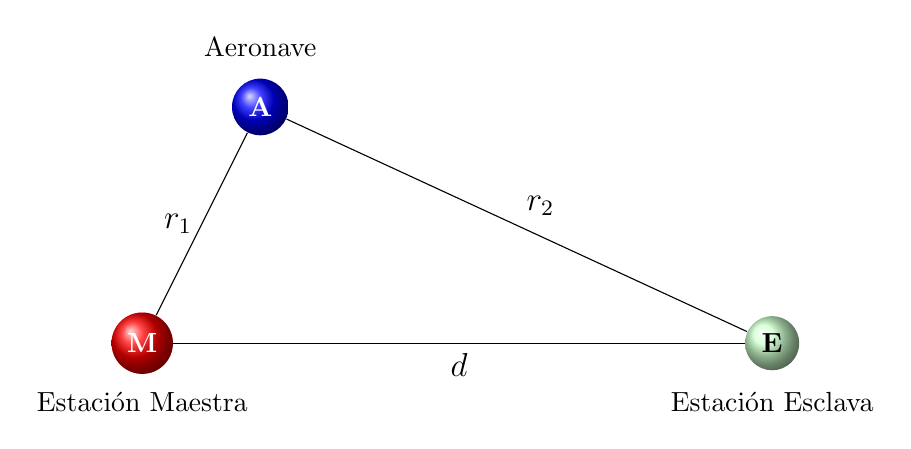
\begin{tikzpicture}[scale=1]
%\usetikzlibrary{snakes}
%\usetikzlibrary{calc}

%  \draw[help lines, green!70, step=0.5] (0,0) grid (9,4);
	% Impulso tiempo t0

	\node[circle, 
				shading=ball, 
				fill=red!50, 
				ball color=red,
				text=white
				] (M) at (0,0) {$\bf M$};

	\node[circle,
				shading=ball, 
				ball color=green!20,
%				text=white
				] (E) at (8,0) {$\bf E$};

	\node[circle,
				shading=ball,
%				ball color=black,
				text=white
				] (A) at (1.5,3) {$\bf A$};

	\draw (M) ++(0.0,-0.5) node[anchor=north] {Estaci\'on Maestra}; 
	\draw (E) ++(0.0,-0.5) node[anchor=north] {Estaci\'on Esclava}; 
	\draw (A) ++(0.0,1.0) node[anchor=north] {Aeronave}; 

	\draw (M) -- (A) node[midway, above,anchor=east] {\large $r_1$};
	\draw (E) -- (A) node[midway, above,anchor=south west] {\large $r_2$};
	\draw (M) -- (E) node[midway, above,anchor=north] {\large $d$};

\end{tikzpicture}
    }
%  \caption{Tri\'angulo de situaci\'on}
  \label{fig:06.triangulo.situacion}
 }
 \caption{Navegaci\'on hiperb\'olica}

\end{figure}


\subsubsection{T\'ecnicas de navegaci\'on hiperb\'olica}

Los sistemas hiperb\'olicos solo pueden determinar diferencias de distancias, para ello se emplean dos t\'ecnicas diferentes:

\begin{description}
\item [T\'ecnica de impulsos-tiempos:] conociendo la velocidad de las ondas electromagn\'eticas, $\mathbf{c}$, se puede relacionar el tiempo medido con la distancia recorrida mediante la expresi\'on:

\[ \Delta\,r = c\,\Delta t
\]

De donde:

\[ r = r_0+c\,\left(t-t_0\right)
\]

%\begin{figure}[!h]
% \end{figure}

Pero la ecuaci\'on encierra una gran dificultad de llevar a la pr\'actica puesto que $t_0$ implica conocer el momento exacto en que se produjo la transmisi\'on del emisor. Este problema desaparece si se considera, en lugar de una distancia determinada a una estaci\'on, una diferencia de distancias a dos estaciones puesto que si ambas transmiten sincronizadas, al efectuarse la diferencia de distancia la inc\'onita $t_0$ desaparece.

Para ver con mas detalle lo anterior, consid\'erese una estaci\'on emisora maestra, $M$  que empieza su emisi\'on en el tiempo $t_0$; otra estaci\'on denominada esclava ubicada a una distancia $d$ de la estaci\'on maestra, recibe esta se\~nal luego de un tiempo $d/c$. Luego de un tiempo $\tau$, denominado ``tiempo de sincronismo'', emite una se\~nal id\'entica a la recibida. 

El receptor en la aeronave ($A$) recibe las se\~nales emitidas por las emisoras maestra y esclava, calculando la diferencia de tiempo entre ambas $\Delta\,t = t_2-t_1$. 

Partiendo de la estaci\'on maestra en el tiempo $t_0$, el impulso tarda un tiempo $t_1-t_0$ en llegar al receptor de la aeronave:

\[t_1-t_0 = \displaystyle \frac{r_1}{c}
\]

Al llegar el impulso de la estaci\'on madre a la esclava, esta luego del tiempo $\tau$, emite el suyo el cual llega en el tiempo $t_2$ al receptor, de esta forma se tiene:

\[
t_2-t_0 = \displaystyle \frac{d}{c}+\tau+\frac{r_2}{c}
\]

Haciendo la diferencia de $t_2-t_1$ seg\'un las expresiones anteriores:

\[
t_2-t_1 = t_0 + \displaystyle \frac{d}{c}+\tau+\frac{r_2}{c} - t_0 -\frac{r_1}{c} = \tau+\frac{d+r_2-r_1}{c} = \tau+\frac{d+\Delta\,r}{c}
\]

Finalmente:

\[
\Delta\,t = \tau+\frac{d+\Delta\,r}{c}
\]

Esta expresi\'on implica que a cada incremento de tiempo ($\Delta t$) le corresponde uno de distancia ($\Delta r$), con los par\'ametros $d$, $c$ y $\tau$ conocidos.

Pero debe recordarse algo, en lugar de considerar hip\'erbolas que son curvas planas, este m\'etodo ubica al receptor en un hiperboloide de revoluci\'on. Por esto deben hacerse correcciones por la curvatura y forma de la tierra.


\item [T\'ecnica de onda continua-fases:]

En esta t\'ecnica la emisi\'on es de forma continua a diferencia de la anterior que es por pulsos y que el par\'ametro que se mide es la diferencia de fases.

Se utilizan dos emisores omnidireccionales con un sincronismo de fases entre sus se\~nales. El receptor recibe a ambas se\~nales con una diferencia de fase, que depende de la distancia de la aeronave a cada una de las emisoras. De esta manera se determina la hip\'erbola donde se encuentra el receptor.

Conociendo la longitud de onda $\lambda$ se puede obtener la distancia recorrida seg\'un la fase medida: 

\[\Delta r = \lambda \,\Delta \phi \quad \Longrightarrow r = r_0 +\lambda \,\left( \phi - \phi_0 \right) \]

Aqui se presenta una dificultad porque el receptor necesita conocer $ \phi_0$, la fase exacta en que se produjo la transmisi\'on.

El proceso se realiza de la siguiente forma, la estaci\'on maestra ubicada en $M$ emite su se\~nal continua con frecuencia $f_1$ (longitud de onda $\lambda_1$) y origen de fases $ \phi_{1_0}$. La estaci\'on esclava en $E$ recibe esta se\~nal y transmite la suya con frecuencia $f_2$ y fase inicial $ \phi_{2_0}$. La frecuencia $f_2$ es diferente de la $f_1$ para que el receptor pueda separar facilmente las se\~nales.

La antena de la aeronave recibe ambas se\~nales $f_1$ y $f_2$ con fases $\phi_1$ y $\phi_2$ diferentes a las de salida, cuyos valores son:

\[
\phi_1 = {\phi_1}_0 + \displaystyle \frac{r_1}{\lambda_1} \qquad
\phi_2 = {\phi_2}_0 + \displaystyle \frac{r_2}{\lambda_2} 
\]

Para poder comparar estas se\~nales se usa el artificio de una frecuencia com\'un, $f_c$, con longitud de onda $\lambda_c$ que resulta de multiplicar a cada una de las frecuencias anteriores por un n\'umero entero $n_1$ y $n_2$, respectivamente:

\[
f_c = n_1\,f_1 = n_2\,f_2
\]

Cuando se multiplica una frecuencia por un n\'umero, se hace lo mismo con su fase, por lo que las expresiones anteriores vistas desde esta frecuencia com\'un, quedan:

\[
\theta_1 = n_1\,\phi_1 = n_1\,{\phi_1}_0 + \displaystyle \frac{n_1\,r_1}{\lambda_1} \qquad
\theta_2 = n_2\,\phi_2 = n_2\,{\phi_2}_0 + \displaystyle \frac{n_2\,r_2}{\lambda_2} 
\]

Restando la diferencia de las fases:

\[
\Delta\,\theta = \theta_1-\theta_2 = n_1\,{\phi_1}_0 + \displaystyle \frac{n_1\,r_1}{\lambda_1} -  n_2\,{\phi_2}_0 - \displaystyle \frac{n_2\,r_2}{\lambda_2} 
\]

El sincronismo de fase entre la estaci\'on maestra y la esclava debe realizarse de forma que se cumpla lo siguiente:

\begin{itemize}
\item La diferencia de fases iniciales multiplicadas por su entero respectivo debe mantenerse constante: $n_1\,{\phi_1}_0- n_2\,{\phi_2}_0= cte$

\item El ajuste de sincronismo que realiza la estaci\'on esclava cumple, en la prolongaci\'on de la l\'inea que la une con la maestra pero en el lado de la maestra, que la diferencia de fases en la aeronave sea nula: 

Para $r_1=0$ y $r_2=d$ se cumple que $\Delta\,\theta = \theta_1-\theta_2 =0$

\end{itemize}

Sabiendo que para un lado se cumple $c = f_c\,\lambda_c = f_1\,\lambda_1$ y como $f_c=n_1\,f_1$, entonces $n_1f_1\lambda_c = f_1\lambda_1$, por lo que $n_1\lambda_c=\lambda_1$ o $\displaystyle \frac{n_1}{\lambda_1}=\frac{1}{\lambda_c}$.

De la misma manera se obtiene $\displaystyle \frac{n_2}{\lambda_2}=\frac{1}{\lambda_c}$.

Volviendo a la diferencia de fases de la frecuencia com\'un:

\[
\Delta\,\theta = n_1\,{\phi_1}_0- n_2\,{\phi_2}_0 +  \displaystyle \frac{n_1\,r_1}{\lambda_1}  - \displaystyle \frac{n_2\,r_2}{\lambda_2}= cte + \frac{\Delta r}{\lambda_c}
\]

Trabajando con la expresi\'on anterior se llega a que:

\[
\Delta \theta = \displaystyle \frac{d+\Delta r}{\lambda_c}
\]

Surge un problema adicional, esta expresi\'on solo resuelve el incremento de fase dentro de una longitud de onda determinada pero se desconoce dentro de cual. 
Esto resulta en una indeterminaci\'on m\'ultiple, ya que el \'angulo real ser\'a un n\'umero entero de longitudes de onda m\'as el desfase obtenido de la ecuaci\'on anterior. 
La indeterminaci\'on ser\'a mayor cuanto mayor sea la frecuencia de la se\~nal radiada (menor $\lambda$). 
El inconveniente se soluciona con otra t\'ecnica conocida como del n\'umero de longitudes de onda completas.


\end{description}


\subsection{LORAN}
\label{sec:06.loran}

%Ver la siguiente pagina, de donde sacaron la informacion los de Alaca
%http://jproc.ca/hyperbolic/loran_c.html


El \textbf{LORAN} (del ingl\'es LOng RAnge Navigation, navegaci\'on de largo alcance) es un sistema de ayuda a la navegaci\'on electr\'onica de tipo hiperb\'olico
 de largo alcance, que opera en baja y media frecuencia. 

Utiliza el intervalo transcurrido entre la recepci\'on de se\~nales de radio transmitidas desde tres o m\'as transmisores para determinar la posici\'on del receptor. 

Desarrollado a principios de la II Guerra Mundial, el LORAN fue el primer sistema de navegaci\'on basado en la llegada diferenciada de se\~nales de radio. Fue concebido por el laboratorio de Radiaci\'on de MIT. LORAN fue, tambi\'en, el primer sistema de posicionamiento capaz de funcionar bajo cualquier condici\'on climatol\'ogica pero es solamente bidimensional (latitud y longitud).

\begin{figure}[!tbh]
  \centering
  \subfigure[Interior de la instalaci\'on emisora]{\includegraphics[height=5.5cm]{06.radionavegacion/Imagenes/06.01.adf/LORAN-Equip-Hut_.jpg}}
  \subfigure[Vista de estaci\'on emisora]{\includegraphics[height=5.5cm]{06.radionavegacion/Imagenes/06.01.adf/LORAN-A_1940-instalacion-terrestre.jpg}}
  \caption{Instalaciones de LORAN-A \protect\cite{Historia_LORAN} }
\end{figure}

 El sistema emisor LORAN se compone de una estaci\'on maestra y otras esclavas. La maestra emite de forma regular una peque\~na se\~nal, que es repetida por la esclava, controlada por radio desde la maestra.
En la Figura \ref{fig:06.loran.cadenas} puede observarse la configuraci\'on t\'ipica de cadenas LORAN (Maestra + Esclavas) y una cadena ubicada en USA.

 Ambas se\~nales se reciben en el barco o avi\'on, se amplifican y se registran. Los circuitos del receptor est\'an dispuestos de forma que la distancia entre las se\~nales corresponda a la diferencia de tiempos de llegada de las se\~nales de ambas estaciones. El receptor posee adem\'as un dispositivo temporizador electr\'onico que permite medir dicha diferencia en microsegundos (millon\'esimas de segundo). 

En la Figura \ref{fig:06.loran.vista.detallada.pulso.y.gri} puede observase un detalle del pulso emitido en la se\~nal LORAN y del \ac{GRI}.

% \begin{landscape}
   \begin{figure}[!h]
     \centering
     \subfigure[Configuraciones t\'ipicas de cadenas LORAN]{\includegraphics[width=0.5\textwidth]{06.radionavegacion/Imagenes/06.01.Loran/configuracion_cadenas_Loran.png}}
     \subfigure[Cadena LORAN GRI 9960]{\includegraphics[width=0.5\textwidth]{06.radionavegacion/Imagenes/06.01.Loran/Loran_cadena_GRI_9960.png}}
     \caption{Cadenas LORAN \protect\cite{LoranC_user_book}}
     \label{fig:06.loran.cadenas}
   \end{figure}

% \end{landscape}
 
% \begin{figure}[!h]
%      \centering
%      \includegraphics[width=\textwidth]{06.radionavegacion/Imagenes/06.01.Loran/Loran_vista_detallada_pulso_+GRI.png}
%      \caption{Vista detallada de un pulso y de GRI \protect\cite{LoranC_user_book}}
%      \label{fig:06.loran.vista.detallada.pulso.y.gri}
%    \end{figure}





Como las ondas de radio viajan a una velocidad aproximadamente constante de 3$ \times 10^8$ m/segundo, la ubicaci\'on de todos los puntos en los que las se\~nales de las dos estaciones est\'an separadas un determinado intervalo de tiempo se puede representar mediante una curva concreta que es una hip\'erbola (Figura \ref{fig:LORAN_hiperbolas}). El navegante dispone de un mapa con muchas de estas curvas, denominadas curvas de posici\'on LORAN, y tras determinar la diferencia de tiempos, por ejemplo, 3 $\mu$segundos, sabe que la posici\'on de su nave se halla en alg\'un punto de la curva de 3 $\mu$segundos del mapa. Sintonizando una pareja de emisores LORAN y repitiendo este proceso, el navegante es capaz de detectar otra curva que represente la posici\'on de la nave, la posici\'on real de la aeronave se halla en la intersecci\'on de las dos curvas LORAN. 


\begin{figure}[!h]
  \centering
  \includegraphics[width=0.8\textwidth ]{06.radionavegacion/Imagenes/06.01.Loran/06_Loran_intersecciones.png}
  \caption{Mapa de hip\'erbolas del sistema LORAN, (A) Estación Maestra, (B) Estación Esclava, $\tau=1$mseg, tiempos en mseg \protect\cite{tooley2017aircraft}}
  \label{fig:LORAN_hiperbolas}
\end{figure}


Este sistema pose\'ia un alcance \'util de unos 2592,8 km (1400 nm) por la noche y unos 1296,4 km (700 nm) de d\'ia,
ver Figuras \ref{fig:06.LoranC.alcances}. 
%Las se\~nales se emitían generalmente en la banda de frecuencias de 1,8 a 2,0 MHz. 
Sirvi\'o tanto para marcar y mantener un rumbo, como para fijar la posici\'on, y presentaba la ventaja de ser independiente de las condiciones meteorol\'ogicas. Su exactitud oscilaba entre unos centenares de metros y unos pocos kil\'ometros, dependiendo del equipo utilizado y de la distancia entre la nave y la emisora. 

La versi\'on m\'as moderna fu\'e LORAN-C que oper\'o en frecuencias del espectro electromagn\'etico entre 90 y 110 Khz (la portadora es 100 kHz para todas las estaciones). El sistema LORAN fu\'e utilizado en muchos pa\'ises, entre ellos los Estados Unidos de Am\'erica, Jap\'on y varios pa\'ises europeos. Rusia utiliz\'o un sistema casi id\'entico llamado CHAYKA, que emple\'o la misma banda de frecuencias. 

\begin{figure}[!h]
  \centering
  \subfigure[Alcance de VOR y DME]{ \includegraphics[height=18em]{06.radionavegacion/Imagenes/06.01.Loran/06_VOR+DME_cobertura_marDelNorte.png}}\hspace{1em}
  \subfigure[Alcance de Loran C]{ \includegraphics[height=18em]{06.radionavegacion/Imagenes/06.01.Loran/06_LoranC_cobertura_marDelNorte.png}}
  \caption{Comparación de alcances de sistema VOR+DME y Loran-C \protect\cite{tooley2017aircraft}}
  \label{fig:06.LoranC.alcances}
\end{figure}



% From  Tooley Aircraft communications
%
% The intention for a Loran-C system is to only use ground waves for navigation purposes; sky waves are filtered out with pulse timing techniques. The approximate time taken for a transmitted wave to reflect off the ionosphere is 30 ms; since the pulse duration is 270 ms some of the transmitted pulse can be expected to be reflected from the ionosphere. To avoid this, a specific peak within the pulse is selected as the indexing pulse. This is the third peak within the pulse and represents approximately 50% of the maximum amplitude.

% Signals are transmitted from the master station as a group of nine pulses; secondary stations transmit eight pulses, see Figure 14.6. Groups of pulses from each of the chains are transmitted within the range of 10–25 groups per second. Each pulse is spaced at 1 ms intervals; the ninth pulse from the master station occurs after a 2 ms delay. The specific timing interval of the group of pulses (starting and finishing with the master pulses) is referred to as the group repetition interval, or GRI. This time interval is used as the basis of identifying the chain, e.g. a chain with
% GRI of 99,600 microseconds is identified as ``9960''.

% The first group of nine pulses from the master station is received at different times by each of the secondary stations due to the varying baseline distances between respective stations. The secondary stations transmit their pulse groups after predetermined time delays, referred to as the coding delay. The total time for the pulse to travel over the baseline together with the secondary station’s coding delay is called the emission delay. 

% Operational aspects associated with Loran-C include:
% electromagnetic interference affecting the signal, e.g. from power lines loss of one station affecting the area of
% coverage local weather conditions (particularly electrical storms) affecting the signal. 

% In addition to master and secondary stations, monitoring stations are deployed to sample the chain’s signal strength, timing and pulse shape.

% In the event that any of these are outside a specified limit, an alert signal, known as a blink, is coded into the pulse groupings.

\begin{minipage}[c]{0.65\linewidth}
  El Loran-C utiliza ondas terrestres únicamente para fines de
  navegación pero las ondas del cielo pueden interferir por lo cual se
  las filtra con técnicas de sincronización de pulsos.  Una onda
  transmitida tarda en reflejarse en reflejarse en la ionosfera
  aproximadamente 30 mseg, el pulso de Loran-C es de 270 mseg por lo
  que se puede esperar que parte del pulso transmitido se refleje
  desde la ionosfera.  Para evitar esto se selecciona un pico
  específico dentro del pulso como ``\emph{pulso de indexación}'' el
  cual es el tercer pico dentro del pulso y representa aproximadamente
  el 50\% de la amplitud máxima, ver Figura \ref{fig:06.LoranC.formato.pulsos}.
\end{minipage}\hspace{1em}
\begin{minipage}[c]{0.30\linewidth}
  \includegraphics[width=\linewidth]{06.radionavegacion/Imagenes/06.01.Loran/06_LoranC_pulso_formato.png}
  \captionof{figure}{Formato de pulso de Loran-C \protect\cite{tooley2017aircraft}}
  \label{fig:06.LoranC.formato.pulsos}

\end{minipage}

Desde la estación Maestra las señales se transmiten  como un grupo de nueve pulsos mientras que las estaciones secundarias transmiten ocho pulsos, Figura \ref{fig:06.LoranC.secuencia.pulsos}. Los grupos de pulsos de cada una de las cadenas se transmiten dentro del rango de 10 a 25 grupos por segundo. Cada pulso está espaciado a intervalos de 1 mseg; el noveno pulso de la estación maestra ocurre después de un retraso de 2 mseg. El intervalo de tiempo específico del grupo de pulsos (comenzando y terminando con los pulsos maestros) se denomina Intervalo de Repetición de Grupo o Group Repetition Interval (GRI). Este intervalo de tiempo se utiliza como base para identificar la cadena. 
%p. Ej. una cadena con el GRI de 99,600 microsegundos se identifica como `` 9960 ''.

\begin{figure}[!h]
  \centering
  \includegraphics[width=\linewidth]{06.radionavegacion/Imagenes/06.01.Loran/06_LoranC_pulsos_secuencia.png}
  \caption{Intervalo de Repetición de Grupo (GRI) de Loran-C \protect\cite{tooley2017aircraft}}
  \label{fig:06.LoranC.secuencia.pulsos}
\end{figure}

El primer grupo de nueve pulsos de la estación maestra es recibido en diferentes momentos por cada una de las estaciones secundarias debido a las diferentes distancias de línea de base entre las respectivas estaciones. Las estaciones secundarias transmiten sus grupos de pulsos después de retardos de tiempo predeterminados, denominados retardo de codificación. El tiempo total que tarda el pulso en viajar sobre la línea de base junto con el retardo de codificación de la estación secundaria se denomina retardo de emisión.

Los aspectos operativos asociados con Loran-C incluyen:
\begin{itemize}
\item Interferencia electromagnética que afecta a la señal, p. ej. por la presencia de líneas eléctricas.
\item Pérdida de la señal de  una estación que afecta el área
  de cobertura
\item Condiciones meteorológicas severas (particularmente tormentas eléctricas) que afecten a la señal.

\end{itemize}

Además de las estaciones maestra y secundaria se emplean  estaciones de monitoreo  para muestrear la intensidad de la señal de la cadena, el tiempo y la forma del pulso emitido.
Si alguno de estos parámetros se encuentre fuera de un límite especificado, se codifica una señal de alerta, conocida como {\bf blink} (parpadeo) en las agrupaciones de pulsos.



A fin de proporcionar una protección contra la interferencia de fuentes externas y también reducir la contaminación de la onda de tierra 
%de los pulsos transmitidos después 
de las ondas celestes,
% de los pulsos precedentes 
se empleó la codificaci\'on por fase de los pulsos. 
Dado que la onda de cielo del primer pulso llega al receptor al mismo tiempo que la onda de tierra del segundo pulso por lo que esta contaminación 
por ondas del cielo  sin codificación de fase anularía el efecto de muestrear solo la onda terrestre, degradando así la precisión inherente del sistema.

Además, el uso de la codificación de fase también proporciona al receptor la información lógica necesaria para la búsqueda automática de las señales maestra y esclavas. La búsqueda automática se puede utilizar por conveniencia o cuando la relación señal / ruido de las señales recibidas impide la identificación visual.

 
% El uso de pulsos codificados por fase por parte del sistema proporciona una medida de protección contra la interferencia de fuentes externas y también reduce la contaminación de la onda terrestre de los pulsos transmitidos después de las ondas celestes de los pulsos precedentes; es decir, la onda del cielo del primer pulso llega al mismo tiempo que la onda de tierra del segundo pulso. La contaminación por ondas del cielo precedentes sin codificación de fase anularía el efecto de muestrear solo la onda terrestre, degradando así la precisión inherente del sistema. El uso de la codificación de fase también proporciona al receptor la información lógica necesaria para la búsqueda automática de las señales maestra y esclava. La búsqueda automática se puede utilizar por conveniencia o cuando la relación señal / ruido de las señales recibidas impide la identificación visual.


%Within each of these multi-pulse groups from the master and slave stations, the phase of the RF carrier is changed with respect to the pulse envelope in a systematic manner from pulse-to-pulse. The phase of each pulse in an eight or nine-pulse group is changed in accordance with a prescribed code so that it is either in phase (+) or 180? out of phase (-) with a stable 100 kc/s reference signal. The phase code used at a master station is different from the phase code used at a slave, but all slave stations use the same code and currently (1962) all LORAN-C chains use the same code. The sequence utilized in a typical LORAN-C star chain is given below:

Para realizar la codificaci\'on anterior,  la fase de la portadora de RF se cambia con respecto a la envolvente de pulso de manera sistemática de pulso a pulso. 
La secuencia utilizada en una típica cadena LORAN-C se muestra en la Tabla \ref{tab:06.Loran.C.secuencia.cambio.fase}.
La fase de cada pulso en un grupo de ocho o nueve pulsos se cambia de acuerdo con un código prescrito para que esté en fase indicado con el s\'imbolo (+) o 180º fuera de fase indicado con el s\'imbolo (-), con una señal de referencia estable de 100 kHz. 
El código de fase en una estación maestra es diferente del de una esclava, ver 
Tabla \ref{tab:06.Loran.C.secuencia.cambio.fase}.


\begin{table}[!h]
  \centering
\caption{Secuencia de cambio de fase Loran-C \protect\cite{Loran1962}}
\label{tab:06.Loran.C.secuencia.cambio.fase}
% ver pagina 69 de la referencia
  \begin{tabular}{lcccc} \hline
  &MASTER &X-SLAVE& Y-SLAVE& Z-SLAVE \\ \hline
Primer per\'iodo repetici\'on &+ - - +++++ &+ - + - ++- - &+ - + - ++ - - &+ - + - ++ - - \\ 
Segundo per\'iodo repetici\'on &++ - - +-+- &+++++ - - + &+++++ - -+ &+++++ - - + \\
Tercer per\'iodo repetici\'on & \multicolumn{4}{c}{Idem Primer per\'iodo repetici\'on}\\
Cuarto per\'iodo repetici\'on & \multicolumn{4}{c}{Idem Segundo per\'iodo repetici\'on}\\
& \multicolumn{4}{c}{Etc.} \\ \hline
\end{tabular}
\end{table}

%The use of phase-coded pulses by the system provides a measure of protection against interference from outside sources and also reduces contamination of the groundwave of pulses transmitted subsequent to skywaves from preceding pulses; i.e., skywave of the first pulse arriving at the same time as the groundwave of the second pulse. Contamination by preceding skywaves without phase coding would nullify the effect of sampling only the groundwave, thereby degrading the inherent accuracy of the system. The use of phase coding also provides the receiver with necessary logical information for automatic search for the master and slave signals. Automatic search can be utilized for convenience or when the signal- to-noise ratio of the received signals precludes visual identification.




\begin{landscape}


\Informacion{¿El fin del LORAN?}{

  \begin{small}
    El uso de LORAN ha dejado de ser utilizado al ser reeplazado por
    GPS. Sin embargo, debido a la interferencia que se puede producir
    en \'este \'ultimo sistema se ha estudiado la posibilidad de
    mejorar y volver a popularizar este sistema mediane el eLORAN. Ver
    el siguiente art\'iculo 
      \href{https://rntfnd.org/2018/06/06/russia-china-upgrading-loran-eloran-systems/}{\bf
        Russia, China Upgrading Loran/ eLoran Systems?}
%	\href{https://rntfnd.org/2020/08/27/eloran-and-aviation-aviation-policy-news/}{}
  \end{small}
}






  \begin{figure}[!tbh]
    \centering
    \includegraphics[width=\textwidth]{06.radionavegacion/Imagenes/06.01.Loran/06_Loran_cobertura.jpg}
    \caption{ Cobertura LORAN.  
{\scriptsize Fuente: \url{https://www.reddit.com/r/MapPorn/comments/3aaak8/station_location_and_coverage_areas_of_the_loran/}}     }
    \label{fig:LORAN-A-cobertura-1973}
  \end{figure}

\end{landscape}







\section{ADF}
%\section{ADF, función, diagrama en bloque, principio de funcionamiento}
\label{sec:U06.01.ADF}

% Versión 2021
%
\begin{tcolorbox}{Conceptos b\'asicos del sistema \ac{ADF}}

  \begin{itemize}
  \item El \ac{ADF}, es uno de los sistemas de radio navegación mas
    antiguos, est\'a compuesto por un equipo llevado a bordo de la
    aeronave y otros en tierra.

  \item La funci\'on del ADF es indicar al piloto la direcci\'on en la
    cual se encuentra una \ac{NDB} sintonizada.

  \item La \ac{NDB} es la correspondiente radioayuda en tierra que se
    sintoniza, mientras que el ADF es el equipo a bordo de la
    aeronave. El ADF puede utilizar se\~nales de otras fuentes, como
    radioemisoras comerciales.

  \item A nivel mundial, se utiliza el ancho de banda entre 200 kHz y
    1750 kHz (aunque los l\'imites pueden variar un poco seg\'un el
    lugar). En Europa los NDB t\'ipicamente se encuentran en las
    sub-bandas 255-415 y 510-525 kHz.

  \item Este rango de frecuencias coloca al sistema en el dominio de la
    \ac{MF}, entre las  ondas ionosf\'ericas (o de
    cielo) y las ondas de tierra. Estas \'ultimas son capaces de llegar a
    largas distancias y sobrepasar obst\'aculos.

  \item La longitud de onda es bastante grande
    comparada con las dimensiones de una aeronave: f = 200 kHz -
    $\lambda = 1500$ m, y f = 1750 kHz - $\lambda = 171.429$ m.

  \item La se\~nal se emite en \ac{AM},envi\'andose la
    identificaci\'on de la estaci\'on NDB en c\'odigo Morse
    o m\'usica y sonidos en el caso de las radioemisoras comerciales.

  \item El alcance es de 25 a 100 NM (46,3 a 185,2 km), puede ser
    mayor, pero aparecen problemas.

  \item La intensidad de campo requerida es de 70 $\mu$Voltios/m, con
    S/N $>$ 15 dB.

  \item La precisi\'on media obtenida es de 3º a 5º en condiciones
    normales de operaci\'on.

  \item La polarizaci\'on es vertical con propagaci\'on horizontal.
  \end{itemize}

\end{tcolorbox}

\subsection{Antena de cuadro}
\label{sec:06.antena.de.cuadro}

La antena de cuadro (tambi\'en llamada antena loop), es una evoluci\'on de las antenas ``Adcock'' que consiste en dos antenas verticales aisladas conectadas en contrafase, ver Figura \ref{fig:antena.adcock}.

La antena de cuadro tiene las antenas verticales conectadas entre s\'i y est\'a hecha de varias vueltas de hilo conductor para mejorar sus propiedades de recepci\'on, como se muestra en la Figura \ref{fig:antena.cuadro}.

Las dos secciones verticales de la antena son las que reciben la se\~nal, son paralelas entre s\'i y est\'an conectadas en ``contrafase'', lo que significa que lo que reciben se resta entre s\'i y lo que sale es la diferencia.

\begin{figure}[!h]
  \centering
 \subfigure[Antena Adcock %\\ {\tiny Fuente:\url{http://www.flyingstart.ca/FlightTraining/preflight/antennae.html}}
	]{
	 \includegraphics[width=0.4\textwidth]{06.radionavegacion/Imagenes/06.01.adf/adcock-antena-01.jpg}
	 \label{fig:antena.adcock}
	 }
% \subfigure[Antigua antena de cuadro ubicada en la parte baja del fuselaje de un DC3.\\ {\tiny Fuente:armyintelligence.tpub.com/IT0302/IT03020036.htm}]{\includegraphics[height=6.5cm]{Imagenes/06.01.adf/DC3-loop-antena.jpg}  \label{fig:antena.loop.vieja}}
 \subfigure[Antigua antena de cuadro ubicada en la parte baja del fuselaje de un DC3]{\includegraphics[width=0.4\textwidth]{06.radionavegacion/Imagenes/06.01.adf/DC3-loop-antena.jpg}  \label{fig:antena.loop.vieja}}
  \caption{Antenas}
\end{figure}




\subsection{Radiogoni\'ometro}

La evoluci\'on del ADF ha sido en fases. La primera de ellas fue el radiogoni\'ometro, que hallaba la direcci\'on en la cual se encontraba una estaci\'on emisora en tierra, pero NO lo hac\'ia de manera autom\'atica.

Este instrumento ten\'ia una antena de cuadro que pod\'ia girarse manualmente desde la cabina, como la mostrada en la Figura \ref{fig:antena.loop.vieja}.

El siguiente dibujo representa una antena de cuadro cuyo plano est\'a inclinado un cierto \'angulo $\theta$ con respecto al origen de la se\~nal:


\begin{figure}[!h]
  \centering
\subfigure[Antena de cuadro \protect\cite{ADF-teoria}]{  \includegraphics[width=0.3\textwidth]{06.radionavegacion/Imagenes/06.01.adf/antena-cuadro.png}  \label{fig:antena.cuadro}}
\subfigure[Recepci\'on de la se\~nal por la antena de cuadro \protect\cite{ADF-teoria}]{  \includegraphics[width=0.6\textwidth]{06.radionavegacion/Imagenes/06.01.adf/antena-cuadro-recibiendo-senial.png}  \label{fig:antena.cuadro.recibiendo.senial}}
  \caption{Antena de cuadro}
\end{figure}


En la Figura \ref{fig:antena.cuadro.recibiendo.senial} se puede apreciar claramente que debido a que la ``Antena 1'' (Ant. 1 en la figura) y la ``Antena 2'' (Ant. 2) est\'an separadas una cierta distancia y, adem\'as, existe un \'angulo entre la se\~nal que llega y el plano que une las antenas ($\theta$), la primera recibe la se\~nal antes que la segunda. Por esto existe un desfase entre ambas, y por tanto una diferencia (la salida de la antena de cuadro NO es cero en este caso).

 En la Figura \ref{fig:seniales.recibidas.antena.cuadro} se ilustra la forma de las se\~nales recibidas por la antena 1 ($y_1$), la antena 2 ($y_2$) y la diferencia entre ellas ( $y_3 = y_2 - y_1$ ), que es realmente la salida de la antena de cuadro.

\begin{figure}[!h]
  \centering
  \subfigure[Se\~nales recibidas por la antena de cuadro ]{  \includegraphics[, height=6cm]{06.radionavegacion/Imagenes/06.01.adf/adf-seniales-antena-cuadro.eps}  \label{fig:seniales.recibidas.antena.cuadro}}
  \subfigure[Se\~nales recibidas por la antena de cuadro ]{  \includegraphics[height=6cm]{06.radionavegacion/Imagenes/06.01.adf/diagrama-recepcion-antena-cuadro.png}  \label{fig:diagrama.recepcion.antena.cuadro}}

  \caption{Esquemas funcionamiento antena de cuadro}
\end{figure}

En la Figura \ref{fig:diagrama.recepcion.antena.cuadro} se muestra un diagrama de recepci\'on de estas antenas, el resultado es una figura de ``ocho'', donde la recepci\'on es mayor cuando la se\~nal llega paralela al plano de la antena de cuadro, y nula cuando viene perpendicularmente.


Esta caracter\'istica es aprovechada para hallar la direcci\'on de donde proviene la se\~nal. El ``radionavegante'' a bordo del avi\'on ten\'ia en su panel de control una ruedecilla (acoplada a un indicador de direcci\'on) con la que pod\'ia girar a voluntad (y manualmente) la antena de cuadro, mientras simult\'aneamente escuchaba con sus aud\'ifonos la se\~nal de audio proveniente del emisor (NDB o estaci\'on de radio comercial).

Cuando el radionavegante dejaba de escuchar la se\~nal significaba que el plano de la antena de cuadro estaba perpendicular a la direcci\'on en la cual se encontraba el emisor, tomando nota de dicha direcci\'on (mostrada en el indicador) y marc\'andola en su carta de navegaci\'on.

El m\'etodo anterior encuentra la direcci\'on pero \emph{existe una ambigüedad en el sentido}, pues el emisor puede estar a un lado u otro del plano de la antena de cuadro. Esta ambigüedad era resuelta tomando otros emisores como referencia, y hallando la intersecci\'on de las direcciones, o llevando un registro cuidadoso de la trayectoria del avi\'on desde el inicio del vuelo.

En la Figura \ref{fig:diag-bloques-radiogoniometro} se ilustra el diagrama de bloques del radiogoni\'ometro.


\begin{figure}[!h]
  \centering
   \includegraphics[width=0.5\textwidth]{06.radionavegacion/Imagenes/06.01.adf/diag-bloques-radiogoniometro.png}
  \caption{Diagrama de bloques del radiogoni\'ometro}
  \label{fig:diag-bloques-radiogoniometro}
\end{figure}


En un circuito aparte, alimentado por una ``\emph{antena de referencia}'', proporciona una se\~nal en el sistema de audio que no est\'a sometida a las variaciones de amplitud que implica el cambio de direcci\'on de la antena de cuadro.



\subsection{ADF}

La diferencia principal entre el radiogoni\'ometro y el ADF es que este \'ultimo es \emph{autom\'atico}, como lo indica su nombre. Esto indica que la ambigüedad en el sentido debe resolverse dentro del propio equipo.

Para ello, se instala una antena de referencia que, por comodidad, se representar\'a en el centro de la antena de cuadro. La se\~nal recibida por esta antena se considera que no tiene desfase y al graficarla en el tiempo ($y_4$) estar\'a entre $y_1$ y $y_2$, ver Figura \ref{fig:seniales-2}.


\begin{figure}[!h]
  \centering
  \subfigure[Se\~nales recibidas por la antena de cuadro + se\~nal de referencia. ]{  \includegraphics[width=0.45\textwidth]{06.radionavegacion/Imagenes/06.01.adf/adf-+seniales-antena-cuadro.eps}  \label{fig:seniales-2}}
  \subfigure[Se\~nales antena de cuadro + referencia + referencia desfasada 90º. ]{  \includegraphics[width=0.45\textwidth]{06.radionavegacion/Imagenes/06.01.adf/senyales-3.png}  \label{fig:seniales-3}}

  \subfigure[Diagrama de recepci\'on antena de cuadro + antena de referencia.]{  \includegraphics[width=0.65\textwidth]{06.radionavegacion/Imagenes/06.01.adf/diag-recepcion-2.png}  \label{fig:diag-recepcion-2}}

  \caption{Se\~nales recibidas por la antena de cuadro}
\end{figure}


Si la se\~nal de referencia se desfasa 90º (en la Figura \ref{fig:seniales-3} se indica como curva $y_5$), se puede apreciar que pr\'acticamente entra en fase con $y_3$, la cual es la salida de la antena de cuadro cuando la antena 1 est\'a m\'as cerca del emisor que la antena 2. Correspondientemente, $y_5$ estar\'a en contrafase con $y_3$ si es la antena 2 la que est\'a m\'as cerca del emisor ($y_6 = y_1 - y_2$). %Lo anterior se representa en la Figura \ref{fig:seniales-3}. 

Esta caracter\'istica de la recepci\'on se aprovecha para determinar el sentido en el que se encuentra el sector y as\'i resolver la ambigüedad que padec\'ia el radiogoni\'ometro. Si se hace un diagrama de recepci\'on de la combinaci\'on antena de cuadro + antena de referencia, se obtiene un diagrama de radiaci\'on en forma de curva \emph{cardioide}, ver Figura \ref{fig:diag-recepcion-2}.


Entonces, la se\~nal de la antena de cuadro es introducida alternativamente a dos combinadores que generan 2 cardioides: Uno recibe $y_3$ ($y_2-y_1$) y el otro $y_6$ ($y_1-y_2$). \'Estos a su vez tambi\'en reciben $y_5$ y la salida de ambos alimenta a un comparador.

El resultado de la comparaci\'on es amplificado y alimenta a su vez al motor que mueve el cuadro. Este motor girar\'a en un sentido u otro seg\'un el signo de la comparaci\'on dejando de mover la antena cuando la se\~nal de ambas cardioides resulte igual. Un acoplador selsyn conectado al motor del cuadro transmite la se\~nal hasta un indicador en la cabina de vuelo.

En la Figura \ref{fig:diag-bloques-adf-rot} se presenta el diagrama de bloques de lo anterior.

% \begin{figure}[!h]
%   \centering
%   \includegraphics[width=0.75\textwidth]{06.radionavegacion/Imagenes/06.01.adf/diag-bloques-adf-rot.png}   
%   \label{fig:diag-bloques-adf-rot}
%   \caption{Diagrama  de bloques del ADF con antena rotatoria}
% \end{figure}


%\begin{landscape}
 
 \begin{figure}[!h]
    \centering \subfigure[Diagrama de bloques del ADF con antena
    rotatoria]{ \includegraphics[width=0.45\textwidth]{06.radionavegacion/Imagenes/06.01.adf/diag-bloques-adf-rot.png} \label{fig:diag-bloques-adf-rot}}
    \subfigure[Diagrama de bloques del ADF con antena
    rotatoria]{ \includegraphics[width=0.45\textwidth]{06.radionavegacion/Imagenes/06.01.adf/esquema-adf-rot.png} \label{fig:esquema-adf-rot}}
    \caption{}
  \end{figure}


%\end{landscape}

El siguiente esquema muestra las cardioides que el comparador est\'a recibiendo de los combinadores y c\'omo el sistema reacciona seg\'un cada caso, ver Figura \ref{fig:esquema-adf-rot}.

%\subsubsection{Reacciones del sistema ADF con antena rotatoria}

Para explicar estas reacciones vamos a estudiarlas por casos, siempre teniendo en cuenta que la flecha denotada como ``\emph{Sentido de la medida}'' representa la flecha del indicador:

\begin{description}
\item[\bf Emisor en posici\'on A:] En este caso, la cardioide 1 ($C_11$) es mayor que la cardioide 2 ($C_2$), $C_1 > C_2$ lo que hace que el comparador emita una se\~nal al motor del cuadro que har\'a rotar al conjunto COMO LAS AGUJAS DEL RELOJ (unos 150º en este caso) hasta que la flecha apunte hacia ``A''. Cuando se llegue a ese punto, $C_1=C_2$ y se detendr\'a el movimiento.


\item[\bf Emisor en posici\'on B:] Ahora el comparador hallar\'a que $C_2 > C_1$, y por tanto dar\'a al motor del cuadro la orden de giro AL CONTRARIO DE LAS AGUJAS DEL RELOJ hasta que la flecha apunte hacia ``\emph{B}'', lugar en donde se detiene el giro porque $C_1 = C_2$.
    

\item[\bf Emisor en posici\'on X:] En este caso no hay movimiento porque la estaci\'on est\'a precisamente en donde $C_1 = C_2$. No obstante, si por alguna desviaci\'on de la aeronave resulta que la flecha apuntara brevemente un poco ``\emph{por debajo}'' de ``\emph{X}'', entonces $C_1 > C_2$ y el motor empezar\'a a girar como las agujas del reloj, lo que posicionar\'a la flecha otra vez en ``X''. Si por el contrario la flecha apuntara brevemente ``\emph{por encima}'' de ``\emph{X}'', entonces $C_2 > C_1$ y el motor girar\'ia al rev\'es del reloj, volviendo a colocar la flecha apuntando a ``\emph{X}''. En definitiva, esta posici\'on es de equilibrio estable.


\item[\bf Emisor en posici\'on C:] Esta posici\'on representa aparentemente un problema porque la estaci\'on est\'a situada justamente al contrario de lo indicado por la flecha, pero como $C_1 = C_2$ en teor\'ia la aguja permanecer\'ia en la posici\'on err\'onea. Sin embargo, la m\'as ligera desviaci\'on de esta posici\'on provocar\'ia que el conjunto diera una vuelta de 180º, colocando a la flecha en la posici\'on correcta. Por ejemplo, si C se mueve relativamente un poco hacia abajo de abajo de la posici\'on actual, $C_2 > C_1$ y la antena se mover\'ia al contrario del reloj, aumentando a cada momento la diferencia entre $C_2$ y $C_1$, hasta que se d\'e una vuelta completa y se encuentre de nuevo el equilibrio, ahora con la flecha apuntando en el sentido correcto. Por tanto, la posici\'on ``C'' es de ``\emph{equilibrio inestable}'' y no representa un problema en la pr\'actica.
 
\end{description}
    

Conforme evolucion\'o la tecnolog\'ia, se encontraron maneras de desarrollar un sistema ADF que resolviera la ambigüedad de sentido sin necesidad de rotar la antena de cuadro, mejor\'andose la confiabilidad del sistema.

Para ello, se utilizan dos antenas de cuadro colocadas ortogonalmente. La que tiene su plano a lo largo del eje longitudinal del avi\'on (adelante-atr\'as) es la ``\textbf{antena coseno}'', mientras aquella cuyo plano coincide con el eje transversal es la ``\textbf{antena seno}'', ver Figura \ref{fig:esquema-adf-fijo}.

De esta manera se tienen dos diagramas de recepci\'on en ``\emph{ocho}'', perpendiculares entre s\'i, que generar\'an sus respectivas cardioides al ser adecuadamente combinados con la se\~nal proveniente de la antena de referencia.% Observe el siguiente diagrama:



De forma an\'aloga al caso del ADF con antena rotatoria, las se\~nales provenientes de las antenas de cuadro son combinadas con la se\~nal de la antena de referencia y alimentan alternativamente (con una frecuencia de alternancia de 100 Hz) a un comparador de fases. La salida de \'este son los valores de seno y coseno del \'angulo $\theta$ entre el eje longitudinal del avi\'on y la posici\'on de la estaci\'on.

Estas se\~nales seno-coseno alimentan a los indicadores (por ejemplo, un Indicador Radio-Magn\'etico o RMI), o a trav\'es de una interfaz ARINC 429 a un bus de datos digital.

En la Figura \ref{fig:diag-bloques-adf-fijo} se encuentra el diagrama de bloques t\'ipico de este sistema.

\begin{figure}[!h]
  \centering
  \subfigure[Diagrama de las antenas de cuadro ortogonales]{\includegraphics[width=0.75\textwidth]{06.radionavegacion/Imagenes/06.01.adf/esquema-adf-fijo.png}\label{fig:esquema-adf-fijo}}
  \subfigure[Diagrama de bloques del ADF con antenas fijas]{\includegraphics[width=0.75\textwidth]{06.radionavegacion/Imagenes/06.01.adf/diag-bloques-adf-fijo.png}\label{fig:diag-bloques-adf-fijo}}
  \caption{ADF fijo}
\end{figure}

\Informacion{Antenas para ADF}{
En el \href{https://www.sensorantennas.com/product/adf-antenna/}{siguiente link} puede accederse a una antena ADF comercial.

\href{http://verdanttelemetry.com/products-list.php?prdtcat_id=148}{Otro link} con informaci\'on de antenas ADF.
}



\subsubsection{NDB}
Como se indic\'o previamente, el NDB es la radioayuda en tierra que corresponde al ADF. Las sub-bandas de frecuencia usadas en Europa para los NDB t\'ipicamente se encuentran entre 255-415 y 510-525 kHz. Los NDB modulan en AM su identificaci\'on de estaci\'on en c\'odigo Morse, compuesta usualmente por tres letras.

\begin{figure}[!h]
  \centering
  \subfigure[S\'imbolo NDB usado en cartas aeron\'auticas ]{\includegraphics[width=0.15\textwidth]{06.radionavegacion/Imagenes/06.01.adf/NDB-simbolo.png}\label{fig:simbolo_ndb}} 
	\hspace{20pt}
  \subfigure[Emisor NDB en 49º 12.35' N, 2º 13.20' W. Callsign JW - 'Jersey West'. 329.0 kHz]{\includegraphics[width=0.25\textwidth]{06.radionavegacion/Imagenes/06.01.adf/NDB-transmisor.jpg}\label{fig:imagen_ndb}}
  \caption{NDB}
\end{figure}


Estos radiofaros con emisi\'on omnidirecciona en azimut tienen la caracter\'istica que sus antenas no pueden radiar en su direcci\'on longitudinal, por lo cual justo por encima de los NDBs se forma un cono en el cual NO existe se\~nal.

Este cono, caracter\'istico tambi\'en de otras radioayudas, es llamado ``cono de silencio'', y su \'angulo de abertura puede tener, en el caso de los NDB, hasta 45º.

El alcance de los NDB puede ir desde unas 25 NM (46300\,m) hasta m\'as de 100 NM (185200 m), dependiendo de la potencia de emisi\'on. M\'as all\'a de las 100 NM (185200 m) empiezan a aparecer importantes errores.

\Informacion{Estaciones NDB en Argentina}{
  Por el
  \href{http://186.153.175.229/descarga/aip-5b6deb26b09dd}{siguiente link}
  puede accederse a una lista de las estaciones NDB y otras radioayudas disponibles en Argentina en el a\~no 2018.
}

%\begin{landscape}
  \subsubsection{Presentaci\'on de la informaci\'on}
  \label{sec:06.adf.presentacion.informacion}

  % \url{https://greatbustardsflight.blogspot.com/2019/09/indicador-de-direccion-df-direction.html}

  % \begin{figure}[!h]
  %   \centering
  %   \subfigure[RBI]{\includegraphics[width=0.3\textwidth]{06.radionavegacion/Imagenes/06.01.adf/RBI-0001.jpg}}
  %   \subfigure[RBI]{\includegraphics[width=0.4\textwidth]{06.radionavegacion/Imagenes/06.01.adf/RMI.jpg}}
  %   \subfigure[RMI +
  %   VOR]{\includegraphics[width=0.25\textwidth]{06.radionavegacion/Imagenes/06.01.adf/rmi-adf-vor.png}}
  %   \caption{Formas de presentaci\'on de la informaci\'on}
  %   \label{fig:06.RBI.RMI}
  % \end{figure}

La informaci\'on presentada al piloto puede ser en forma de \ac{RBI} (Figura \ref{fig:06.RBI}) o como \ac{RMI} (Figura \ref{fig:06.RMI}), donde tambi\'en se presenta el QDM (rumbo magn\'etico a una estaci\'on),ver Figura  \ref{fig:06.QDM}. 

\begin{figure}[!h]
  \centering
  \subfigure[ADF]{\includegraphics[width=0.4\textwidth]{06.radionavegacion/Imagenes/06.01.adf/adf-1.jpg} \label{fig:06.RBI}}
  \subfigure[QDM]{\includegraphics[width=0.25\textwidth]{06.radionavegacion/Imagenes/06.01.adf/QDM.jpg} \label{fig:06.QDM}}

  \subfigure[ADF]{\includegraphics[width=0.6\textwidth]{06.radionavegacion/Imagenes/06.01.adf/adf-2.jpg} \label{fig:06.RMI}}
  \caption{Formas de presentaci\'on de la informaci\'on \protect\cite{QDM-RBI-RMI}}
  \label{fig:06.RBI.RMI}
\end{figure}

%\end{landscape}



\subsubsection{Errores ADF-NDB}

El sistema ADF/NDB tiene errores que t\'ipicamente oscilan entre los 3º y 5º. Hay dos tipos principales de error que son:

\begin{description}
\item [Errores Sistem\'aticos]

Los errores sistem\'aticos se pueden caracterizar previamente y tomar previsiones ante ellos. Los m\'as importantes son:

\begin{description}
\item [Error Instrumental]

Es el error asociado a incertidumbres en la lectura de los valores mostrados por los instrumentos. Oscila de 1 a 2 grados.

\item [Error por presencia del avi\'on]

La aeronave es un cuerpo met\'alico que puede interferir con la recepci\'on del sistema, distorsionando las se\~nales. Sin embargo, este error puede caracterizarse de f\'abrica y entonces tomar medidas correctivas.

\end{description}


\item [Errores Variables]

Como su nombre lo indica, son errores cuya aparici\'on y magnitud depende de m\'ultiples factores, siendo esencialmente desconocidos. Los m\'as conocidos son:

\begin{description}

\item [Errores atmosf\'ericos (tormentas)]

El n\'ucleo de las grandes tormentas genera poderosas cargas electromagn\'eticas cuya frecuencia puede estar en la banda de trabajo del ADF. Esto ocasiona que las tormentas puedan aparecer como estaciones en tierra y el ADF apuntar\'a hacia ellas. Es muy peligroso que el piloto las confunda con estaciones reales y vuele hacia ellas.


\item [Errores de polarizaci\'on]

Ciertas condiciones pueden alterar la polarizaci\'on y propagaci\'on de las se\~nales y ocasionar errores. Las m\'as conocidas son:

\begin{description}
\item [Efecto de l\'inea de costa], causado por la diferente conductividad entre la corteza terrestre y el agua, ocasionando que la se\~nal se refracte al pasar por la costa y genere indicaciones erradas.


\item [Efecto monta\~na], en donde debido a la orograf\'ia las ondas de tierra se pueden distorsionar, apareciendo errores de medici\'on.

\end{description}


\item [Interferencia xDSL (en estudio)]

La transmisi\'on de datos por Internet utilizando la tecnolog\'ia xDSL (HDSL, SDSL, VDSL y ADSL) puede generar se\~nales que interfieran con la operaci\'on del ADF y con las comunicaciones HF.

Debido a la naturaleza de los sistemas xDSL la fuente de interferencia est\'a distribuida geogr\'aficamente. Se est\'an realizando estudios para determinar si el efecto acumulativo de muchas de estas se\~nales puede alterar seriamente el funcionamiento del sistema (referencia actualizada al 21/Sep/2000).


\item [Efecto FADING]

Este efecto de ``desvanecimiento'' aparece porque a cierta distancia de la estaci\'on emisora las ``ondas de suelo'' y las ``ondas de cielo'' (estas \'ultimas por rebote ionosf\'erico) empiezan a interferir entre s\'i.
\vspace{10pt}

\begin{minipage}[b]{0.5\linewidth}
La interferencia entre ambas se\~nales puede ser constructiva o destructiva seg\'un el desfase que exista entre ellas, produci\'endose el efecto de una recepci\'on err\'atica e intermitente.

El siguiente gr\'afico representa la intensidad de campo versus la distancia a la estaci\'on, indicando las zonas en donde es m\'as probable que ocurra este efecto.
Una observaci\'on final es que durante la noche y cuando la aeronave se aproxima al ``terminator'' (l\'inea divisoria entre el d\'ia y la noche) es m\'as probable que se produzca este efecto, debido a la variaci\'on en la altura de la ionosfera.

\end{minipage}
\begin{minipage}[b]{0.5\linewidth}
  % \begin{figure}[!htb]
  \centering
  \includegraphics[width=\linewidth]{06.radionavegacion/Imagenes/06.01.adf/grafico-fading.png}
%  \captionof{ Gr\'afico del efecto ``fading''}
  \label{fig:fading}
%\end{figure}  
\end{minipage}





\end{description}

\end{description}






% \begin{tcolorbox}{Conceptos b\'asicos del sistema \ac{ADF}}

%   \begin{itemize}
%   \item El \ac{ADF}, es uno de los sistemas de radio navegación mas
%     antiguos, est\'a compuesto por un equipo llevado a bordo de la
%     aeronave y otros en tierra.

%   \item La funci\'on del ADF es indicar al piloto la direcci\'on en la
%     cual se encuentra una \ac{NDB} sintonizada.

%   \item La \ac{NDB} es la correspondiente radioayuda en tierra que se
%     sintoniza, mientras que el ADF es el equipo a bordo de la
%     aeronave. El ADF puede utilizar se\~nales de otras fuentes, como
%     radioemisoras comerciales.

%   \item A nivel mundial, se utiliza el ancho de banda entre 200 kHz y
%     1750 kHz (aunque los l\'imites pueden variar un poco seg\'un el
%     lugar). En Europa los NDB t\'ipicamente se encuentran en las
%     sub-bandas 255-415 y 510-525 kHz.

%   \item Este rango de frecuencias coloca al sistema en el dominio de la
%     \ac{MF}, entre las  ondas ionosf\'ericas (o de
%     cielo) y las ondas de tierra. Estas \'ultimas son capaces de llegar a
%     largas distancias y sobrepasar obst\'aculos.

%   \item La longitud de onda es bastante grande
%     comparada con las dimensiones de una aeronave: f = 200 kHz -
%     $\lambda = 1500$ m, y f = 1750 kHz - $\lambda = 171.429$ m.

%   \item La se\~nal se emite en \ac{AM},envi\'andose la
%     identificaci\'on de la estaci\'on NDB en c\'odigo Morse
%     o m\'usica y sonidos en el caso de las radioemisoras comerciales.

%   \item El alcance es de 25 a 100 NM (46,3 a 185,2 km), puede ser
%     mayor, pero aparecen problemas.

%   \item La intensidad de campo requerida es de 70 $\mu$Voltios/m, con
%     S/N $>$ 15 dB.

%   \item La precisi\'on media obtenida es de 3º a 5º en condiciones
%     normales de operaci\'on.

%   \item La polarizaci\'on es vertical con propagaci\'on horizontal.
%   \end{itemize}

% \end{tcolorbox}

% \subsection{Antena de cuadro}
% \label{sec:06.antena.de.cuadro}

% La antena de cuadro (tambi\'en llamada antena loop), es una evoluci\'on de las antenas ``Adcock'' que consiste en dos antenas verticales aisladas conectadas en contrafase, ver Figura \ref{fig:antena.adcock}.

% La antena de cuadro tiene las antenas verticales conectadas entre s\'i y est\'a hecha de varias vueltas de hilo conductor para mejorar sus propiedades de recepci\'on, como se muestra en la Figura \ref{fig:antena.cuadro}.

% Las dos secciones verticales de la antena son las que reciben la se\~nal, son paralelas entre s\'i y est\'an conectadas en ``contrafase'', lo que significa que lo que reciben se resta entre s\'i y lo que sale es la diferencia.

% \begin{figure}[!h]
%   \centering
%  \subfigure[Antena Adcock %\\ {\tiny Fuente:\url{http://www.flyingstart.ca/FlightTraining/preflight/antennae.html}}
% 	]{
% 	 \includegraphics[width=0.4\textwidth]{06.radionavegacion/Imagenes/06.01.adf/adcock-antena-01.jpg}
% 	 \label{fig:antena.adcock}
% 	 }
% % \subfigure[Antigua antena de cuadro ubicada en la parte baja del fuselaje de un DC3.\\ {\tiny Fuente:armyintelligence.tpub.com/IT0302/IT03020036.htm}]{\includegraphics[height=6.5cm]{Imagenes/06.01.adf/DC3-loop-antena.jpg}  \label{fig:antena.loop.vieja}}
%  \subfigure[Antigua antena de cuadro ubicada en la parte baja del fuselaje de un DC3]{\includegraphics[width=0.4\textwidth]{06.radionavegacion/Imagenes/06.01.adf/DC3-loop-antena.jpg}  \label{fig:antena.loop.vieja}}
%   \caption{Antenas}
% \end{figure}




% \subsection{Radiogoni\'ometro}

% La evoluci\'on del ADF ha sido en fases. La primera de ellas fue el radiogoni\'ometro, que hallaba la direcci\'on en la cual se encontraba una estaci\'on emisora en tierra, pero NO lo hac\'ia de manera autom\'atica.

% Este instrumento ten\'ia una antena de cuadro que pod\'ia girarse manualmente desde la cabina, como la mostrada en la Figura \ref{fig:antena.loop.vieja}.

% El siguiente dibujo representa una antena de cuadro cuyo plano est\'a inclinado un cierto \'angulo $\theta$ con respecto al origen de la se\~nal:


% \begin{figure}[!h]
%   \centering
% \subfigure[Antena de cuadro \protect\cite{ADF-teoria}]{  \includegraphics[width=0.3\textwidth]{06.radionavegacion/Imagenes/06.01.adf/antena-cuadro.png}  \label{fig:antena.cuadro}}
% \subfigure[Recepci\'on de la se\~nal por la antena de cuadro \protect\cite{ADF-teoria}]{  \includegraphics[width=0.6\textwidth]{06.radionavegacion/Imagenes/06.01.adf/antena-cuadro-recibiendo-senial.png}  \label{fig:antena.cuadro.recibiendo.senial}}
%   \caption{Antena de cuadro}
% \end{figure}


% En la Figura \ref{fig:antena.cuadro.recibiendo.senial} se puede apreciar claramente que debido a que la ``Antena 1'' (Ant. 1 en la figura) y la ``Antena 2'' (Ant. 2) est\'an separadas una cierta distancia y, adem\'as, existe un \'angulo entre la se\~nal que llega y el plano que une las antenas ($\theta$), la primera recibe la se\~nal antes que la segunda. Por esto existe un desfase entre ambas, y por tanto una diferencia (la salida de la antena de cuadro NO es cero en este caso).

%  En la Figura \ref{fig:seniales.recibidas.antena.cuadro} se ilustra la forma de las se\~nales recibidas por la antena 1 ($y_1$), la antena 2 ($y_2$) y la diferencia entre ellas ( $y_3 = y_2 - y_1$ ), que es realmente la salida de la antena de cuadro.

% \begin{figure}[!h]
%   \centering
%   \subfigure[Se\~nales recibidas por la antena de cuadro ]{  \includegraphics[, height=6cm]{06.radionavegacion/Imagenes/06.01.adf/adf-seniales-antena-cuadro.eps}  \label{fig:seniales.recibidas.antena.cuadro}}
%   \subfigure[Se\~nales recibidas por la antena de cuadro ]{  \includegraphics[height=6cm]{06.radionavegacion/Imagenes/06.01.adf/diagrama-recepcion-antena-cuadro.png}  \label{fig:diagrama.recepcion.antena.cuadro}}

%   \caption{Esquemas funcionamiento antena de cuadro}
% \end{figure}

% En la Figura \ref{fig:diagrama.recepcion.antena.cuadro} se muestra un diagrama de recepci\'on de estas antenas, el resultado es una figura de ``ocho'', donde la recepci\'on es mayor cuando la se\~nal llega paralela al plano de la antena de cuadro, y nula cuando viene perpendicularmente.


% Esta caracter\'istica es aprovechada para hallar la direcci\'on de donde proviene la se\~nal. El ``radionavegante'' a bordo del avi\'on ten\'ia en su panel de control una ruedecilla (acoplada a un indicador de direcci\'on) con la que pod\'ia girar a voluntad (y manualmente) la antena de cuadro, mientras simult\'aneamente escuchaba con sus aud\'ifonos la se\~nal de audio proveniente del emisor (NDB o estaci\'on de radio comercial).

% Cuando el radionavegante dejaba de escuchar la se\~nal significaba que el plano de la antena de cuadro estaba perpendicular a la direcci\'on en la cual se encontraba el emisor, tomando nota de dicha direcci\'on (mostrada en el indicador) y marc\'andola en su carta de navegaci\'on.

% El m\'etodo anterior encuentra la direcci\'on pero \emph{existe una ambigüedad en el sentido}, pues el emisor puede estar a un lado u otro del plano de la antena de cuadro. Esta ambigüedad era resuelta tomando otros emisores como referencia, y hayando la intersecci\'on de las direcciones, o llevando un registro cuidadoso de la trayectoria del avi\'on desde el inicio del vuelo.

% En la Figura \ref{fig:diag-bloques-radiogoniometro} se ilustra el diagrama de bloques del radiogoni\'ometro.


% \begin{figure}[!h]
%   \centering
%    \includegraphics[width=0.5\textwidth]{06.radionavegacion/Imagenes/06.01.adf/diag-bloques-radiogoniometro.png}
%   \caption{Diagrama de bloques del radiogoni\'ometro}
%   \label{fig:diag-bloques-radiogoniometro}
% \end{figure}


% En un circuito aparte, alimentado por una ``\emph{antena de referencia}'', proporciona una se\~nal en el sistema de audio que no est\'a sometida a las variaciones de amplitud que implica el cambio de direcci\'on de la antena de cuadro.



% \subsection{ADF}

% La diferencia principal entre el radiogoni\'ometro y el ADF es que este \'ultimo es \emph{autom\'atico}, como lo indica su nombre. Esto indica que la ambigüedad en el sentido debe resolverse dentro del propio equipo.

% Para ello, se instala una antena de referencia que, por comodidad, se representar\'a en el centro de la antena de cuadro. La se\~nal recibida por esta antena se considera que no tiene desfase y al graficarla en el tiempo ($y_4$) estar\'a entre $y_1$ y $y_2$, ver Figura \ref{fig:seniales-2}.


% \begin{figure}[!h]
%   \centering
%   \subfigure[Se\~nales recibidas por la antena de cuadro + se\~nal de referencia. ]{  \includegraphics[width=0.45\textwidth]{06.radionavegacion/Imagenes/06.01.adf/adf-+seniales-antena-cuadro.eps}  \label{fig:seniales-2}}
%   \subfigure[Se\~nales antena de cuadro + referencia + referencia desfasada 90º. ]{  \includegraphics[width=0.45\textwidth]{06.radionavegacion/Imagenes/06.01.adf/senyales-3.png}  \label{fig:seniales-3}}

%   \subfigure[Diagrama de recepci\'on antena de cuadro + antena de referencia.]{  \includegraphics[width=0.65\textwidth]{06.radionavegacion/Imagenes/06.01.adf/diag-recepcion-2.png}  \label{fig:diag-recepcion-2}}

%   \caption{Se\~nales recibidas por la antena de cuadro}
% \end{figure}


% Si la se\~nal de referencia se desfasa 90º (en la Figura \ref{fig:seniales-3} se indica como curva $y_5$), se puede apreciar que pr\'acticamente entra en fase con $y_3$, la cual es la salida de la antena de cuadro cuando la antena 1 est\'a m\'as cerca del emisor que la antena 2. Correspondientemente, $y_5$ estar\'a en contrafase con $y_3$ si es la antena 2 la que est\'a m\'as cerca del emisor ($y_6 = y_1 - y_2$). %Lo anterior se representa en la Figura \ref{fig:seniales-3}. 

% Esta caracter\'istica de la recepci\'on se aprovecha para determinar el sentido en el que se encuentra el sector y as\'i resolver la ambigüedad que padec\'ia el radiogoni\'ometro. Si se hace un diagrama de recepci\'on de la combinaci\'on antena de cuadro + antena de referencia, se obtiene un diagrama de radiaci\'on en forma de curva \emph{cardioide}, ver Figura \ref{fig:diag-recepcion-2}.


% Entonces, la se\~nal de la antena de cuadro es introducida alternativamente a dos combinadores que generan 2 cardioides: Uno recibe $y_3$ ($y_2-y_1$) y el otro $y_6$ ($y_1-y_2$). \'Estos a su vez tambi\'en reciben $y_5$ y la salida de ambos alimenta a un comparador.

% El resultado de la comparaci\'on es amplificado y alimenta a su vez al motor que mueve el cuadro. Este motor girar\'a en un sentido u otro seg\'un el signo de la comparaci\'on dejando de mover la antena cuando la se\~nal de ambas cardioides es igual. Un acoplador selsyn conectado al motor del cuadro transmite la se\~nal hasta un indicador en la cabina de vuelo.

% En la Figura \ref{fig:diag-bloques-adf-rot} se presenta el diagrama de bloques de lo anterior.

% % \begin{figure}[!h]
% %   \centering
% %   \includegraphics[width=0.75\textwidth]{06.radionavegacion/Imagenes/06.01.adf/diag-bloques-adf-rot.png}   
% %   \label{fig:diag-bloques-adf-rot}
% %   \caption{Diagrama  de bloques del ADF con antena rotatoria}
% % \end{figure}


% %\begin{landscape}
 
%  \begin{figure}[!h]
%     \centering \subfigure[Diagrama de bloques del ADF con antena
%     rotatoria]{ \includegraphics[width=0.45\textwidth]{06.radionavegacion/Imagenes/06.01.adf/diag-bloques-adf-rot.png} \label{fig:diag-bloques-adf-rot}}
%     \subfigure[Diagrama de bloques del ADF con antena
%     rotatoria]{ \includegraphics[width=0.45\textwidth]{06.radionavegacion/Imagenes/06.01.adf/esquema-adf-rot.png} \label{fig:esquema-adf-rot}}
%     \caption{}
%   \end{figure}


% %\end{landscape}

% El siguiente esquema muestra las cardioides que el comparador est\'a recibiendo de los combinadores y c\'omo el sistema reacciona seg\'un cada caso, ver Figura \ref{fig:esquema-adf-rot}.

% %\subsubsection{Reacciones del sistema ADF con antena rotatoria}

% Para explicar estas reacciones vamos a estudiarlas por casos, siempre teniendo en cuenta que la flecha denotada como ``\emph{Sentido de la medida}'' representa la flecha del indicador:

% \begin{description}
% \item[\bf Emisor en posici\'on A:] En este caso, la cardioide 1 (C1) es mayor que la cardioide 2 (C2), lo que hace que el comparador emita una se\~nal al motor del cuadro que har\'a rotar al conjunto COMO LAS AGUJAS DEL RELOJ (unos 150º en este caso) hasta que la flecha apunte hacia ``A''. Cuando se llegue a ese punto, $C_1=C_2$ y se detendr\'a el movimiento.


% \item[\bf Emisor en posici\'on B:] Ahora el comparador hallar\'a que C2 > C1, y por tanto dar\'a al motor del cuadro la orden de giro AL CONTRARIO DE LAS AGUJAS DEL RELOJ hasta que la flecha apunte hacia ``\emph{B}'', lugar en donde se detiene el giro porque C1 = C2.
    

% \item[\bf Emisor en posici\'on X:] En este caso no hay movimiento porque la estaci\'on est\'a precisamente en donde C1 = C2. No obstante, si por alguna desviaci\'on de la aeronave resulta que la flecha apuntara brevemente un poco ``\emph{por debajo}'' de ``\emph{X}'', entonces C1 > C2 y el motor empezar\'a a girar como las agujas del reloj, lo que posicionar\'a la flecha otra vez en "X". Si por el contrario la flecha apuntara brevemente ``\emph{por encima}'' de ``\emph{X}'', entonces C2 > C1 y el motor girar\'ia al rev\'es del reloj, volviendo a colocar la flecha apuntando a ``\emph{X}''. En definitiva, esta posici\'on es de equilibrio estable.


% \item[\bf Emisor en posici\'on C:] Esta posici\'on representa aparentemente un problema porque la estaci\'on est\'a situada justamente al contrario de lo indicado por la flecha, pero como C1 = C2 en teor\'ia la aguja permanecer\'ia en la posici\'on err\'onea. Sin embargo, la m\'as ligera desviaci\'on de esta posici\'on provocar\'ia que el conjunto diera una vuelta de 180º, colocando a la flecha en la posici\'on correcta. Por ejemplo, si C se mueve relativamente un poco hacia abajo de abajo de la posici\'on actual, C2 > C1 y la antena se mover\'ia al contrario del reloj, aumentando a cada momento la diferencia entre C2 y C1, hasta que se d\'e una vuelta completa y se encuentre de nuevo el equilibrio, ahora con la flecha apuntando en el sentido correcto. Por tanto, la posici\'on "C" es de "equilibrio inestable" y no representa un problema en la pr\'actica.
 
% \end{description}
    

% Conforme evolucion\'o la tecnolog\'ia, se encontraron maneras de desarrollar un sistema ADF que resolviera la ambigüedad de sentido sin necesidad de rotar la antena de cuadro, mejor\'andose la confiabilidad del sistema.

% Para ello, se utilizan dos antenas de cuadro colocadas ortogonalmente. La que tiene su plano a lo largo del eje longitudinal del avi\'on (adelante-atr\'as) es la ``\textbf{antena coseno}'', mientras aquella cuyo plano coincide con el eje transversal es la ``\textbf{antena seno}'', ver Figura \ref{fig:esquema-adf-fijo}.

% De esta manera se tienen dos diagramas de recepci\'on en ``\emph{ocho}'', perpendiculares entre s\'i, que generar\'an sus respectivas cardioides al ser adecuadamente combinados con la se\~nal proveniente de la antena de referencia.% Observe el siguiente diagrama:



% De forma an\'aloga al caso del ADF con antena rotatoria, las se\~nales provenientes de las antenas de cuadro son combinadas con la se\~nal de la antena de referencia y alimentan alternativamente (con una frecuencia de alternancia de 100 Hz) a un comparador de fases. La salida de \'este son los valores de seno y coseno del \'angulo theta entre el eje longitudinal del avi\'on y la posici\'on de la estaci\'on.

% Estas se\~nales seno-coseno alimentan a los indicadores (por ejemplo, un Indicador Radio-Magn\'etico o RMI), o a trav\'es de una interfaz ARINC 429 a un bus de datos digital.

% En la Figura \ref{fig:diag-bloques-adf-fijo} se encuentra el diagrama de bloques t\'ipico de este sistema.

% \begin{figure}[!h]
%   \centering
%   \subfigure[Diagrama de las antenas de cuadro ortogonales]{\includegraphics[width=0.75\textwidth]{06.radionavegacion/Imagenes/06.01.adf/esquema-adf-fijo.png}\label{fig:esquema-adf-fijo}}
%   \subfigure[Diagrama de bloques del ADF con antenas fijas]{\includegraphics[width=0.75\textwidth]{06.radionavegacion/Imagenes/06.01.adf/diag-bloques-adf-fijo.png}\label{fig:diag-bloques-adf-fijo}}
%   \caption{ADF fijo}
% \end{figure}

% \Informacion{Antenas para ADF}{
% En el \href{https://www.sensorantennas.com/product/adf-antenna/}{siguiente link} puede accederse a una antena ADF comercial.

% \href{http://verdanttelemetry.com/products-list.php?prdtcat_id=148}{Otro link} con informaci\'on de antenas ADF.
% }



% \subsubsection{NDB}
% Como se indic\'o previamente, el NDB es la radioayuda en tierra que corresponde al ADF. Las sub-bandas de frecuencia usadas en Europa para los NDB t\'ipicamente se encuentran entre 255-415 y 510-525 kHz. Los NDB modulan en AM su identificaci\'on de estaci\'on en c\'odigo Morse, compuesta usualmente por tres letras.

% \begin{figure}[!h]
%   \centering
%   \subfigure[S\'imbolo NDB usado en cartas aeron\'auticas ]{\includegraphics[width=0.15\textwidth]{06.radionavegacion/Imagenes/06.01.adf/NDB-simbolo.png}\label{fig:simbolo_ndb}} 
% 	\hspace{20pt}
%   \subfigure[Emisor NDB en 49º 12.35' N, 2º 13.20' W. Callsign JW - 'Jersey West'. 329.0 kHz]{\includegraphics[width=0.25\textwidth]{06.radionavegacion/Imagenes/06.01.adf/NDB-transmisor.jpg}\label{fig:imagen_ndb}}
%   \caption{NDB}
% \end{figure}


% Estos radiofaros con emisi\'on omnidirecciona en azimut tienen la caracter\'istica que sus antenas no pueden radiar en su direcci\'on longitudinal, por lo cual justo por encima de los NDBs se forma un cono en el cual NO existe se\~nal.

% Este cono, caracter\'istico tambi\'en de otras radioayudas, es llamado ``cono de silencio'', y su \'angulo de abertura puede tener, en el caso de los NDB, hasta 45º.

% El alcance de los NDB puede ir desde unas 25 NM ($\Resultado{1852 * 25}{0}$\,m) hasta m\'as de 100 NM, dependiendo de la potencia de emisi\'on. M\'as all\'a de las 100 NM empiezan a aparecer importantes errores.

% \Informacion{Estaciones NDB en Argentina}{
% Por el \href{http://186.153.175.229/descarga/aip-5b6deb26b09dd}{siguiente link} puede accederse a una lista de las estaciones NDB y otras radioayudas disponibles en Argentina en el a\~no 2018.
% }

% %\begin{landscape}
%   \subsubsection{Presentaci\'on de la informaci\'on}
%   \label{sec:06.adf.presentacion.informacion}

%   % \url{https://greatbustardsflight.blogspot.com/2019/09/indicador-de-direccion-df-direction.html}

%   % \begin{figure}[!h]
%   %   \centering
%   %   \subfigure[RBI]{\includegraphics[width=0.3\textwidth]{06.radionavegacion/Imagenes/06.01.adf/RBI-0001.jpg}}
%   %   \subfigure[RBI]{\includegraphics[width=0.4\textwidth]{06.radionavegacion/Imagenes/06.01.adf/RMI.jpg}}
%   %   \subfigure[RMI +
%   %   VOR]{\includegraphics[width=0.25\textwidth]{06.radionavegacion/Imagenes/06.01.adf/rmi-adf-vor.png}}
%   %   \caption{Formas de presentaci\'on de la informaci\'on}
%   %   \label{fig:06.RBI.RMI}
%   % \end{figure}

% La informaci\'on presentada al piloto puede ser en forma de \ac{RBI} (Figura \ref{fig:06.RBI}) o como \ac{RMI} (Figura \ref{fig:06.RMI}), donde tambi\'en se presenta el QDM (rumbo magn\'etico a una estaci\'on),ver Figura  \ref{fig:06.QDM}. 

% \begin{figure}[!h]
%   \centering
%   \subfigure[ADF]{\includegraphics[width=0.4\textwidth]{06.radionavegacion/Imagenes/06.01.adf/adf-1.jpg} \label{fig:06.RBI}}
%   \subfigure[QDM]{\includegraphics[width=0.25\textwidth]{06.radionavegacion/Imagenes/06.01.adf/QDM.jpg} \label{fig:06.QDM}}

%   \subfigure[ADF]{\includegraphics[width=0.6\textwidth]{06.radionavegacion/Imagenes/06.01.adf/adf-2.jpg} \label{fig:06.RMI}}
%   \caption{Formas de presentaci\'on de la informaci\'on \protect\cite{QDM-RBI-RMI}}
%   \label{fig:06.RBI.RMI}
% \end{figure}

% %\end{landscape}



% \subsubsection{Errores ADF-NDB}

% El sistema ADF/NDB tiene errores que t\'ipicamente oscilan entre los 3º y 5º. Hay dos tipos principales de error que son:

% \begin{description}
% \item [Errores Sistem\'aticos]

% Los errores sistem\'aticos se pueden caracterizar previamente y tomar previsiones ante ellos. Los m\'as importantes son:

% \begin{description}
% \item [Error Instrumental]

% Es el error asociado a incertidumbres en la lectura de los valores mostrados por los instrumentos. Oscila de 1 a 2 grados.

% \item [Error por presencia del avi\'on]

% La aeronave es un cuerpo met\'alico que puede interferir con la recepci\'on del sistema, distorsionando las se\~nales. Sin embargo, este error puede caracterizarse de f\'abrica y entonces tomar medidas correctivas.

% \end{description}


% \item [Errores Variables]

% Como su nombre lo indica, son errores cuya aparici\'on y magnitud depende de m\'ultiples factores, siendo esencialmente desconocidos. Los m\'as conocidos son:

% \begin{description}

% \item [Errores atmosf\'ericos (tormentas)]

% El n\'ucleo de las grandes tormentas genera poderosas cargas electromagn\'eticas cuya frecuencia puede estar en la banda de trabajo del ADF. Esto ocasiona que las tormentas puedan aparecer como estaciones en tierra y el ADF apuntar\'a hacia ellas. Es muy peligroso que el piloto las confunda con estaciones reales y vuele hacia ellas.


% \item [Errores de polarizaci\'on]

% Ciertas condiciones pueden alterar la polarizaci\'on y propagaci\'on de las se\~nales y ocasionar errores. Las m\'as conocidas son:

% \begin{description}
% \item [Efecto de l\'inea de costa], causado por la diferente conductividad entre la corteza terrestre y el agua, ocasionando que la se\~nal se refracte al pasar por la costa y genere indicaciones erradas.


% \item [Efecto monta\~na], en donde debido a la orograf\'ia las ondas de tierra se pueden distorsionar, apareciendo errores de medici\'on.

% \end{description}


% \item [Interferencia xDSL (en estudio)]

% La transmisi\'on de datos por Internet utilizando la tecnolog\'ia xDSL (HDSL, SDSL, VDSL y ADSL) puede generar se\~nales que interfieran con la operaci\'on del ADF y con las comunicaciones HF.

% Debido a la naturaleza de los sistemas xDSL la fuente de interferencia est\'a distribuida geogr\'aficamente. Se est\'an realizando estudios para determinar si el efecto acumulativo de muchas de estas se\~nales puede alterar seriamente el funcionamiento del sistema (referencia actualizada al 21/Sep/2000).


% \item [Efecto FADING]

% Este efecto de ``desvanecimiento'' aparece porque a cierta distancia de la estaci\'on emisora las ``ondas de suelo'' y las ``ondas de cielo'' (estas \'ultimas por rebote ionosf\'erico) empiezan a interferir entre s\'i.

% La interferencia entra ambas se\~nales puede ser constructiva o destructiva seg\'un el desfase que exista entre ellas, produci\'endose el efecto de una recepci\'on err\'atica e intermitente.

% El siguiente gr\'afico representa la intensidad de campo versus la distancia a la estaci\'on, indicando las zonas en donde es m\'as probable que ocurra este efecto:

% \begin{figure}[!htb]
%   \centering
%   \includegraphics[width=\textwidth]{06.radionavegacion/Imagenes/06.01.adf/grafico-fading.png}
%   \caption{ Gr\'afico del efecto ``fading''}
%   \label{fig:fading}
% \end{figure}

% Una observaci\'on final es que durante la noche y cuando la aeronave se aproxima al ``terminator'' (l\'inea divisoria entre el d\'ia y la noche) es m\'as probable que se produzca este efecto, debido a la variaci\'on en la altura de la ionosfera.
% \end{description}

% \end{description}





 \newpage 
% \section{VOR, función, diagrama en bloque, principio de funcionamiento}
% \label{sec:U06.02.VOR}

\section{VOR}
\label{sec:06.VOR}

% 2023
% Unidad 06
% VOR



\subsection{Un poco de historia....}
\label{sec:06.VOR.historia}

% \begin{wrapfigure}{r}{0.35\textwidth} \centering
%   \includegraphics[keepaspectratio,width=0.3\textwidth]{06.radionavegacion/Imagenes/06.02.vor.imagenes/Marconi.eps}\caption{Guillermo Marconi}
% \end{wrapfigure}
 \begin{minipage}[c]{0.55\linewidth}

Las radioayudas utilizadas actualmente (VOR, DME, ILS, etc.) se remontan a los primeros d\'ias de la radiocomunicaci\'on. Sus l\'ineas de origen se cruzan en muchos puntos, pero  encuentran, finalmente, su inicio en dos patentes registradas en Alemania en 1906.

Hacia 1905 Marconi hab\'ia dedicado un esfuerzo considerable a la investigaci\'on de las propiedades de la cl\'asica antena en L invertida. Encontr\'o que si el tramo horizontal era considerablemente mayor que el vertical, el diagrama polar presentaba un abombamiento considerable en la direcci\'on contraria a la l\'inea de secci\'on horizontal.

En 1905 patent\'o un sistema que utilizaba este tipo de antenas tanto para la emisi\'on como la recepci\'on, reivindicando excepcionales propiedades direccionales para la combinaci\'on. Bas\'andose en el mismo principio, Marconi registr\'o al a\~no siguiente la patente de un sistema con un n\'umero de antenas L invertidas igualmente espaciadas en forma radial alrededor del receptor. Seleccionando la antena que recib\'ia la se\~nal m\'as intensa pod\'ia averiguarse la direcci\'on aproximada de la estaci\'on emisora.

Antes de que pasara un a\~no, Telefunken, en Alemania, hab\'ia introducido una idea muy parecida pero utilizando la parte emisora. Consist\'ia en un emisor que radiaba primero una se\~nal de inicio preestablecida a una antena central omnidireccional, seguida de una segunda emisi\'on en cada una de las 32 antenas espaciadas radialmente alrededor del radiador central omnidireccional y situadas seg\'un las marcaciones de la br\'ujula (Figura \ref{fig:brujula.telefunken}).

Una estaci\'on que desease utilizar la baliza, s\'olo ten\'ia que accionar un cron\'ometro al o\'ir la se\~nal de inicio y detenerlo cuando la se\~nal alcanzaba su m\'axima intensidad. Como ayuda a los usuarios del sistema se dise\~no un reloj especial. Ten\'ia una aguja que completaba una revoluci\'on en 32 segundos y su esfera estaba calibrada seg\'un los puntos de la br\'ujula.

Aunque este sistema no alcanz\'o nunca un uso generalizado, se le puede considerar como el precursor de todos los radiofaros giratorios modernos.


\end{minipage}
\begin{minipage}[c]{0.45\linewidth}
  \begin{center}
  \includegraphics[width= 0.7\linewidth]{06.radionavegacion/Imagenes/06.02.vor.imagenes/Marconi.eps}
  \captionof{figure}{Guillermo Marconi} \label{fig:Marconi}
  \vspace{3mm}
  
  \includegraphics[width=0.9\linewidth]{06.radionavegacion/Imagenes/06.02.vor.imagenes/Telefunken.eps}
  \captionof{figure}{La ``\emph{br\'ujula}''\, Telefunken} \label{fig:brujula.telefunken}
\end{center}
\end{minipage}


\begin{minipage}[c]{0.5\linewidth}
En 1907 Bellini y Tosi presentaron un dise\~no que comprend\'ia dos antenas receptoras de cuadro cruzadas a 90 grados a partir de las cuales se pod\'ia determinar la direcci\'on de las ondas incidentes, mediante la magnitud relativa de las corrientes que se induc\'ian en las antenas (Figura \ref{fig:bellini.y.tosi.principio}). Este sistema alcanz\'o un desarrollo ulterior y, durante la Primera Guerra Mundial (1914-1948), ambos contendientes depositaron una confianza considerable en el mismo. Pese a que una estaci\'on radiogonom\'etrica s\'olo pod\'ia controlar a un avi\'on a la vez y que, a veces, debido a desconocidos fen\'omenos de propagaci\'on, surg\'ian errores posicionales de mas de 50 millas; Von Buttlar-Brandenfels, el \'unico comandante de Zeppelin que vol\'o durante toda la guerra dedujo que la radionavegaci\'on era muy superior a la navegaci\'on astron\'omica.
\end{minipage}
\begin{minipage}[c]{0.5\linewidth}
\centering
\includegraphics[keepaspectratio,width=0.75\linewidth]{06.radionavegacion/Imagenes/06.02.vor.imagenes/bellinitosiprinciple.jpg}
\captionof{figure}{Principio del equipo de Bellini y Tosi}
\label{fig:bellini.y.tosi.principio}
\end{minipage}

A partir de 1916, Marconi inici\'o el estudio de radioenlaces direccionales de onda corta en una serie de experimentos que fueron llevados a cabo con diversas alternativas en Hendon y Cernavon, a partir de los cuales se desarroll\'o el ``\emph{faro de radioenlaces}'' que fue instalado en 1921 en Inchkeith Island. El hecho m\'as importante en el dise\~no de este equipo fue que \'unicamente pod\'ia generarse un haz suficientemente localizado como para proporcionar una exactitud digna de consideraci\'on, elevando la frecuencia al espectro de VHF. Adem\'as, el dise\~no de los sistemas de manipulaci\'on no permit\'ia que la baliza radiase informaci\'on err\'onea; asimismo el empleo del cron\'ometro se hizo innecesario.


También en 1907, una patente de O. Scheller de la compa\~n\'ia Lorenz, condujo a una l\'inea de desarrollo que, cuando se combin\'o con el radiofaro rotatorio de Marconi, culmin\'o con las radioayudas de hoy en d\'ia.

Era el ``\emph{Indicador de rumbo}'', cuyo fundamento consist\'ia en que dos antenas con diagramas de radiaci\'on que se interceptaban, eran energizadas alternativamente por un \'unico transmisor. La potencia que se enviaba a una antena era utilizada para formar la letra ``\emph{A}'' y la otra antena formaba la ``\emph{N}''. La posici\'on de las antenas se dispon\'ia de tal manera que la intersecci\'on de sus diagramas de radiaci\'on correspondiese con el rumbo deseado. Por lo tanto, si una aeronave se encontrase fuera de rumbo, recibir\'ia una ``\emph{A}'' o una  ``\emph{N}'', pero si se encontrase en el rumbo, oir\'ia ambas simult\'aneamente, combin\'andose estas para dar un tono continuo.

\begin{figure}[!hbt]
  \centering  \includegraphics[width=0.8\textwidth]{06.radionavegacion/Imagenes/06.02.vor.imagenes/Loran.eps}
    \caption{El sistema de aproximaci\'on de Lorenz.
	(a) Dispositivo de antenas. (b) Modelo de radiaci\'on. \\(c) Diagrama polar vertical y senda de aproximaci\'on.
}
    \label{fig:sistema.lorenz}
\end{figure}

En 1917 se realizaron experiencias en Alemania con barcos y cinco a\~nos m\'as tarde, Keibitz las realiz\'o con aviones. Aunque en tierra se hablaba de un margen de error de 30 m a 3,5 km de distancia, los resultados obtenidos fueron dudosos y la investigaci\'on qued\'o detenida hasta comienzos de la d\'ecada de 1930 cuando la compa\~n\'ia us\'o de nuevo el principio equise\~nal para su equipo de aproximaci\'on de VHF.

Este equipo de aproximaci\'on de Lorenz consist\'ia en un transmisor de VHF situado en la cabecera de la pista de aterrizaje y trabajaba a una frecuencia de aproximadamente 33 Mhz. Este sistema alimentaba un dipolo vertical a cuyos lados, formando \'angulo recto con la pista, se situaba un elemento reflector. El punto medio de cada uno de estos elementos reflectores estaba interrumpido y puenteado por un conjunto de contactos de rel\'e que operaban en oposici\'on, esto es, si un conjunto de contactos se encontraba cerrado el otro estar\'ia abierto, manteniendo sin funcionar ese reflector.

\begin{minipage}[c]{0.5\linewidth}
Operando sobre los rel\'es, el diagrama de radiaci\'on pod\'ia ser trasladado de uno a otro lado. Ambos diagramas se interseccionaban sobre la l\'inea central de la pista  (Figura \ref{fig:sistema.lorenz}). La manipulaci\'on de los receptores se hac\'ia de modo que uno de ellos se manten\'ia en funcionamiento un per\'iodo de tiempo tres veces mayor que el otro; as\'i, cuando un piloto se aproximaba a la pista ligeramente fuera de rumbo, escuchaba una serie de ``\emph{E}'' ($\cdot \, \cdot \, \cdot$) o de ``\emph{T}'' ($- \, - \, -$) que se fund\'ian en un tono continuo ($- \cdot - \cdot - \cdot$) si se encontraba en el rumbo adecuado (Figura \ref{fig:seniales.lorenz}).

\end{minipage}
\begin{minipage}[c]{0.5\linewidth}
\centering
  \includegraphics[width=0.9\linewidth]{06.radionavegacion/Imagenes/06.02.vor.imagenes/Lorenz_beam.png}
  \captionof{figure}{ Se\~nales de Lorenz }
  \label{fig:seniales.lorenz}
\end{minipage}

 Este sistema se denomin\'o \emph{Ultrakurzwellen-Landefunkfeuer} (LFF), o radiobaliza de ondas ultra-cortas para aterrizaje.

El receptor del avi\'on estaba dotado de un medidor de intensidad de se\~nal y pod\'ia obtenerse una gu\'ia de la senda de planeo siguiendo un contorno de igual intensidad de campo.

Este sistema se puso en funcionamiento tambi\'en en Inglaterra con \'exito y se mantuvo en servicio hasta principios de 1960.

En Estados Unidos se investig\'o, por la misma \'epoca, un sistema de antenas ortogonales mediante se\~nales enclavadas. Este m\'etodo generaba cuatro rumbos independientes por cada estaci\'on y se le atribu\'ia una buena apreciaci\'on. 

Desde 1923 a 1926 se continu\'o esta l\'inea, descubri\'endose que utilizando un goni\'ometro transmisor junto con cuadros Bellini-Tosi, los rumbos pod\'ian ser desplazados casi a cualquier direcci\'on deseada. El \'exito del sistema fue tal que a comienzos de 1926 se emprendi\'o la labor de instalar un sistema de estas radiobalizas para trazar el creciente n\'umero de l\'ineas a\'ereas dentro de ese pa\'is. 

Posteriormente se encontr\'o que el sistema de antenas Bellini-Tosi presentaba errores de m\'as de 40 grados en condiciones nocturnas desfavorables, pero su sustituci\'on por antenas Adcock resolvi\'o este problema. En 1944 exist\'ian m\'as de 300 de estos equipos que permanecieron en servicio hasta ser reemplazados por el VOR.


Debido a los problemas inherentes al manejo de radiofaros omnidireccionales de frecuencias medias (efectos nocturnos, etc) en 1937 la U.S. Civil Aeronautics Administration llevó a cabo una serie de pruebas con el uso de VHF para radiofaros omnidireccionales. Las primer las pruebas usaban una frecuencia de 63 MHz y los resultados fueron prometedores, pero surgieron problemas debidos a efectos de reflexión bajo condiciones de propagaci\'on anormales y, en consecuencia, la frecuencia fue elevada a 12S MHz. Aunque todavía subsistían algunos problemas con los sistemas de cuatro rumbos, el trabaJo con VHF había demostrado que el equipo que trabajaba con estas frecuencias era capaz de obtener mejores resultados que el de MF. De todos modos, un problema importante que quedaba por resolver era la desorientación que experimentaba un piloto cuando perdía sus marcaciones cerca de un radiofaro de cuatro rumbos,  por eso se investigó la viabilidad de un sistema de radiofaro de dos rumbos, en el cual se emitian a la vez dos modelos de radiación que conformaban cuatro rumbos distintos. Típicamente podía consistir en un rumbo este-oeste definido por señales de 150 Hz y otro norte-sur de 90 Hz, separándose estas señales mediante filtros en el receptor del avión para alimentar diferencialmente un medidor con el cero en posición central. Esto se conoció como rumbo visual. Adicionalmente se instrumentaron un par de rumbos norte-sur en ángulo recto usando senales interconexionadas del tipo de Lorenz.% (D y U)

Hacia 1936 tambi\'en se consideró un radiofaro que radiaba un n\'umero infinito de rumbos, que era esencialmente un retorno al radiofaro giratorio.

Dicho radiofaro empleaba un sistema en el que el diagrama polar horinzontal tenía forma de cardioide, con la propiedad de que al girar, la intensidad de la señal en cualquier estación receptora variaba sinusoidalmente. El diagrama giraba a 60 Hz. La onda sinusoidal recibida era separada en dos partes en cuadratura de fase, que eran conectadas a las placas
de deflexión de un tubo de rayos catódicos. Esto producia una traza
circular, cada punto de la cual estaba asociado con el instante correspondiente a 
alguna orientaci\'on particular del diagrama espacial, pero sin
ningún punto de referencia. Este fue suministrado al principio introduciendo una discontinuidad en la se\~nal cuando el m\'aximo del diagrama
giratorio pasaba por el norte verdadero, siendo el resultado una deflexi\'on radial en la traza que,
 de otro modo, sería circular, proporcionando así una indicación del rumbo. 

En los primeros trabajos sobre dicho radiofaro se usaba una frecuencîa de 6,5 MHz, 
pero en vista de la tendencia en favor del uso de VHF
cesaron las pruebas con esta frecuencia y posteriormente se usaron frecuencias en la banda de 125 MHz.

Una versi\'on pasterior del equipo sustituía la discontinuidad instantánea de referencia
 por una modulaci\'on a 60 Hz de una subportadora de 10 kHz cuya fase se hacía coincidir con el diagrama
 giratorio en el norte verdadero.

En el receptor se comparaban las fases de la se\~na1 de referencia y de
la se\~nal g\'irada, correspondiendo la diferencia de fase con el rumbo
del receptor. Debido a esta modificaci\'on en la se\~nal de referencia 
se dej\'o de usar como \'indicador el tubo de rayos catódicos, 
que fue sustituido
por un medidor de fase con \'indicac\'i\'on azimutal.

Esto era, en esencia, el VOR que se usa hoy día, consist\'iendo las
principales variaciones posteriores en un cambio en la frecuencia para
usar la banda de 112,0 MHz a 117,9 MHz, en una reducción de la velocidad 
de rotaci\'on del d\'iagrama girator\'io y en una modulación de referenc\'ia
 de 30 Hz usando 9960 Hz para la frecuencia subportadora.

 \begin{myboxRojo}{Desarrollos durante la Segunda Guerra Mundial}

   {\footnotesize   

     \begin{minipage}[c]{0.65\linewidth}

     En el período de este conflicto se produjeron avances notables para el guiado y la navegaci\'on a ciegas de las aeronaves con el fin de realizar bombardeos de precisi\'on. 

Los alemanes utilizaron el principio del sistema de aproximación Lorenz para sus raids de bombardeo a ciegas, principalmente el 
Knickebein (``\emph{Pierna torcida}'') y el X-Ger\"{a}t (``\emph{Aparato-X}''),
durante la ofensiva de bombardeo sobre las ciudades de Inglaterra en el 
invierno de 1940/41.

El X-Ger\"{a}t era muy similar al LFF de Lorenz, siendo mucho m\'as direccional y con mayores alcances. Usando las mismas frecuencias permit\'ia a los aviones utilizar los emisores LFF ya instalados, pero se necesitaba un segundo emisor para ubicar una localizaci\'on.


\end{minipage}
\begin{minipage}[c]{0.35\linewidth}
  \centering
\includegraphics[width=0.9\linewidth]{06.radionavegacion/Imagenes/06.02.vor.imagenes/sottisville-x-geret.jpg}
\captionof{figure}{\footnotesize Modo de uso del X-Ger\"{a}t para posicionar Coventry}
\label{fig:Xgerat}
\end{minipage}


Estos sistemas utilizaban haces cruzados de radiondas de las mismas caracter\'isticas pero de diferentes frecuencias, lo que permit\'ia al piloto calcular su velocidad, desde el momento en que cruzaba la se\~nal y al cruzar la señal principal, luego le indicaba cuando liberar su cargamento.
Los c\'alculos se efectuaban mediante una computadora mec\'anica.

Posteriormente Lorenz modific\'o este sistema creando el sistema de guiado lateral 
Viktoria/Hawaii 
para el misil V-2.

}

\end{myboxRojo}


\subsection{Introducci\'on}
\label{sec:introduccion.vor}

VOR es un acr\'onimo para la frase "\textbf{\textit{VHF Omnidirectional Range}}", que en castellano significa Radiofaro Omnidireccional de VHF. Es un tipo de radioayuda a la navegaci\'on que utilizan las aeronaves para  para delinear aerovías en colaboración con el DME.

Desarrollado en Estados Unidos a partir del radiofaro giratorio de los años veinte, se reconoció como estándar internacional en 1949 y, por lo tanto, ha reemplazado al radiofaro internacional de MF.


\subsection{Principio de funcionamiento}
\label{Principio de funcionamiento}

El principio de funcionamiento del VOR es similar al de un faro de navegaci\'on mar\'itima.

\begin{minipage}[c]{0.6\textwidth}
El faro es una torre alta situada en las costas o en las cercanías de esta, donde se disponen las rutas de navegación de los barcos, que cuenta con un foco de luz muy potente en su parte superior cuya misión es la de guiar por las noches a los navegantes durante sus viajes, es decir, la prinicipal función de un faro es la de guía.

La mencionada lámpara cuenta con lentes de Fresnel que se caracterizan por su gran apertura y una corta distancia focal y cuyos anchos, color y separación variará de acuerdo al faro que se trate.

Mientras el faro está en funcionamiento en la oscuridad la mencionada lámpara emite haces de luz que giran a 360 grados. Entonces, desde la distancia en la cual se encuentren los barcos visualizarán no solamente la luz del faro sino también los colores y los intervalos de haces de luz que presenta la misma. Todo faro tiene su propia frecuencia de emisión de luz que lo hace único. De esta forma los marinos, consultando la correspondiente guía de faros, pueden determinar que faro están viendo y por lo tanto la zona donde navegan.
\end{minipage}
\begin{minipage}[c]{0.4\textwidth}

  \centering
  \includegraphics[width=0.9\linewidth]{06.radionavegacion/Imagenes/06.02.vor.imagenes/faro-alejandria.jpg}
  \captionof{figure}{El faro de Alejadr\'ia \\{\small (reconstrucci\'on)}}
  \label{fig:faro.alejandria}

\end{minipage}

En función de cómo se emite la señal luminosa, los faros se clasifican en: Faro de luz fija, faro de destellos, faro de luz centelleante, faro de grupos de destellos, faro de grupos de ocultaciones, faro de luz alternativa. Según la potencia de luz emitida y la altura en metros sobre el nivel del mar se obtiene el alcance geográfico, que no es más que la distancia máxima a la que se ve la luz que emite.

Los colores universalmente adoptados para emitir luz en los faros son el blanco, verde y rojo. Puede darse el caso, bajo ciertas condiciones atmosféricas, que la luz blanca o la verde adquieran un tono rosado.


El faro es un elemento célebre y útil desde la época de los Romanos, recordado es el faro de Alejandría e incluso esta civilización  supo construir en la entrada de los puertos torres sumamente altas que imitaban de alguna manera al mencionado Faro de Alejandr\'ia (Figura \ref{fig:faro.alejandria}). En el siglo XIX se produciría el gran salto de calidad de los faros con el invento del físico francés Agustin Fresnel. Actualmente los faros son operados a distancia y de manera automática.


El faro más antiguo que se encuentra en funcionamiento es el de la Torre de Hércules ubicado en la península de La Coruña, en Galicia; su alto es de 68 metros, data del siglo I y es el único faro romano en pie.

Volviendo al sistema VOR, la antena de la estaci\'on emite una se\~nal de radiofrecuencia VHF en todas direcciones, que es recibida por el equipo VOR de cualquier aeronave que se encuentre dentro del rango de alcance (max. unos 240 km) y tenga sintonizada la frecuencia de dicha estaci\'on (que puede variar de 108 a 118 MHz).

\begin{figure}[!b]
 \centering
 \subfigure[D-VOR/DME ground station. Identificaci\'on "PEK" (Beijing)]
   {
   \includegraphics[height=5.5cm]{06.radionavegacion/Imagenes/06.02.vor.imagenes/Vor_beijin.jpg}
   \label{fig:Vor_de_Beijin}
   }
 \subfigure[Esquema estaci\'on terrestre]
   {
   \includegraphics[height=5.5cm]{06.radionavegacion/Imagenes/06.02.vor.imagenes/VORGroundStation.jpg}
   \label{fig:Vor.estacion.terrestre}
   }
 \caption{Estaciones VOR }
\end{figure}


La estaci\'on de tierra posee un diagrama de radiaci\'on din\'amico, transmite dos se\~nales VHF en el rango anteriormente mencionado. La radiofrecuencia emitida por un VOR lleva tres se\~nales codificadas. Una es la identificaci\'on de la estaci\'on en c\'odigo Morse \footnote{El c\'odigo Morse es un sistema de representaci\'on de letras y n\'umeros mediante se\~nales emitidas de forma intermitente.}, que permite al piloto saber de cu\'al estaci\'on se trata. Las otras dos son ondas senoidales de 30 Hz cuyas fases var\'ian entre si. Se les llama se\~nal de referencia y se\~nal variable respectivamente. La referencia mantiene siempre su fase constante, mientras que la variable cambia su fase seg\'un la direcci\'on en la que sea emitida. Dicha direcci\'on se mide como un azimut, es decir, se divide en 360 grados alrededor de la antena VOR contando en sentido horario a partir del norte magn\'etico terrestre, punto en el cual la se\~nal de referencia y la variable tienen fase id\'entica. De esta manera se puede visualizar una antena VOR como el punto desde el cual parten 360 l\'ineas de direcci\'on, a las que se les llama radiales.

El equipo VOR en la aeronave recibe la se\~nal VOR y decodifica sus tres se\~nales. Compara la se\~nal de referencia con la variable y determina la diferencia de fase entre las dos. De esta manera puede conocerse en qu\'e radial del VOR sintonizado se encuentra la aeronave con respecto al norte magn\'etico terrestre.

El VOR se utiliza en la aeron\'autica para navegar seg\'un el vuelo IFR \footnote{Recibe el nombre de Reglas de Vuelo Instrumental (m\'as conocido por sus siglas en ingl\'es, IFR), el conjunto de normas y procedimientos recogidos en el Reglamento de Circulaci\'on A\'erea, que regulan el pilotaje de aeronaves en condiciones de visibilidad reducida. Se trata del m\'etodo de navegaci\'on alternativo a las Reglas de Vuelo Visual o VFR.}, siempre permaneciendo en radio con un CTA. Los VOR suelen ir acompa\~nados de DME (Distance Measurement Equipment, Equipo de Medici\'on de Distancia), \'estos son completamente independientes del sistema VOR y ayudan al piloto a saber la distancia que hay entre la aeronave y la estaci\'on VOR. El VOR \'unicamente se utiliza en la llamada "radio navegaci\'on" por lo que siempre hay unos procedimientos que seguir que los marca la carta aeron\'autica para dirijirse a un VOR. Por ejemplo en las SID o salidas normalizadas de un aeropuerto, en la respectiva carta se verifica el procedimiento de apoyo en la salida con los NDB y VOR para poderla realizar correctamente. El piloto debe saber volar bajo reglas de vuelo IFR a un VOR y desde un VOR, o cualquier radioayuda que sea: (NDB, VOR, ILS u otras como el TACAN \footnote{Las siglas TACAN significan  TACtical Air Navigation,  es un tipo de ayuda a la navegaci\'on de uso militar.}) \cite{VOR-Wikipedia}.

Desarrollado de un sistema anterior, Visual-Aural Range (VAR), el VOR se dise\~n\'o para proveer 360 rumbos desde y hacia la estaci\'on seleccionada por el piloto. Los antiguos transmisores de tubo de vac\'io con antenas rotadas mec\'anicamente se instalaron por todos lados en la d\'ecada de 1950 y en la de 1960 comenzaron a ser reemplazados por unidades de estado s\'olido. En este mismo per\'iodo se transformaron en el mayor sistema de navegaci\'on cuando reemplazaron a las viejas radiobalizas. Algunas de estas sobrevivieron como balizas no direccionales de baja o media frecuencia (NDB \footnote{Una Baliza No Direccional,  Non-Directional Beacon (NDB), es una estaci\'on de radio ubicada en un lugar conocido, utilizada como una ayuda para la navegaci\'on a\'erea o naval. Como su nombre implica, la se\~nal no provee informaci\'on direccional en contraste con nuevos tipos de ayudas como VOR. La se\~nal de una NDB copia el contorno de la curvatura de la tierra por lo que puede ser recibida a distancias mayores en latitudes menores, lo que constituye una ventaja sobre el sistema VOR. Sin embargo, la se\~nal NDB es afectada por condiciones atmosf\'ericas, terreno monta\~nosos, refracci\'on costera y tormentas el\'ectricas, particularmente a grandes distancias. A\'un con la aparici\'on de los sistemas VOR y GPS (Global Positioning System), las NDBs contin\'uan siendo las ayudas de navegaci\'on m\'as ampliamente usadas en el mundo. Las NDBs operan en el rango de frecuencias de 190 kHz a 535kHz (aunque tienen frecuencias reservadas en el rango de 190 a 1750 kHz) y una portadora modulada entre  400 o 1020 Hz \cite{NDB}. Entre la informaci\'on transmitida por una NDB se tiene:

\begin{itemize}
 \item Identificaci\'on por c\'odigo Morse entre 400 a 1020 Hz.
\item Informaci\'on de la Terminal A\'erea (Airfield Terminal Information Service = ATIS)
\item Servicio de informaci\'on clim\'atica de la Terminal A\'erea (Airfield Weather Information Service = AWIS), o, en una emergencia un controlador de tr\'afico a\'ereo activando la funci\'on de Presionar-para-hablar (Press-To-Talk = PTT), puede modular la portadora con la voz. El piloto utiliza su receptor ADF para escuchar las instrucciones desde la torre.
\end{itemize}
}).

En los aviones de hoy en d\'ia esto se realiza mediante la FMC, o MCDU seg\'un el fabicante del avi\'on, ya que intoducen directamente la SID y la FMC la realiza automaticamente sola. As\'i podemos llevar a cabo un vuelo, tanto de larga como de corta distancia entre dos puntos del mundo.

En las rutas a\'ereas comerciales m\'as transitadas, al igual que en las carreteras terrestres, hay cruces y curvas. Bajo estos ``\emph{cruces}'' y ``\emph{curvas}'' se suelen instalar estas estaciones VOR. Las ``\emph{carreteras a\'ereas}'' son los radiales de XXX grados que parten de un VOR y que normalmente llegan a otro VOR o incluso a una pista de aterrizaje.

El piloto puede ordenar al piloto autom\'atico: "\textit{Sigua el radial de 115 grados del VOR que transmite en la frecuencia 109.75 Mhz}.", y el avi\'on autom\'aticamente, cuando se cruce con el radial 115, lo seguir\'a hasta sobrevolar el VOR.

\begin{figure} [!hbt]
 \centering
 \includegraphics[width=0.750\textwidth]{06.radionavegacion/Imagenes/06.02.vor.imagenes/mapa_vor.jpg}
 % Mapa_VOR.eps: 0x0 pixel, 300dpi, 0.00x0.00 cm, bb=0 0 500 301
 \caption{Mapa con ruta y posici\'on de estaciones VOR}
 \label{Mapa_estaciones_VOR}
\end{figure}

En el mapa de la Figura  \ref{Mapa_estaciones_VOR} se puede ver una serie de radiobalizas VOR (los c\'irculos grandes) interconectadas entre si por rutas a\'ereas. Cada ruta a\'erea tiene marcado su nombre, altitud y rumbo (que coincide con el radial del VOR del que parte).


\subsection{Equipo de tierra}

\subsubsection{Principios de funcionamiento }

El transmisor es de tipo AM de diseño estándar excepto en el hecho de que el modulador debe ser capaz de trabajar a  frecuencias por encima de los 10 kHz. Para las ayudas en ruta, la potencia de salida es de 200 W, para servicio en aeródromos sólo se necesita 50 W.

La operación de un equipo VOR de tierra está basada en Ia diferencia de fase entre dos señales que emite: una de referencia y otra variable. Cada grado de variación de fase entre las señales, representa un grado de variación de posición del avión.

Los radiales de un VOR son infinitos, pero el equipo de a bordo solo es capaz de diferenciar 360 de ellos.

En una estación VOR, un sistema de monitores y dos transmisores, aseguran un servicio continuo de funcionamiento. Si la señal del equipo se interrumpe por cualquier causa, o varían sus fases, el sistema de monitores desconecta el equipo defectuoso, conectando a su vez un transmisor auxiliar y excitando una alarma en el panel de control que indica un fallo en el sistema. En la Figura \ref{fig:estaciones_VOR}  pueden verse estaciones de tierra. 

\begin{figure}[!htb]
  \centering
  \subfigure[Estación VOR]{\includegraphics[keepaspectratio,height=4.5cm]{06.radionavegacion/Imagenes/06.02.vor.imagenes/Emisor_VOR.eps}}
  \subfigure[Estación VOR Beijin]{\includegraphics[keepaspectratio,height=4.5cm]{06.radionavegacion/Imagenes/06.02.vor.imagenes/Vor_beijin.jpg}}
  \caption{Estaciones VOR}\label{fig:estaciones_VOR}
\end{figure}


El equipo transmisor trabaja en VHF en la banda de 112 Mhz a 118 Mhz, en frecuencias que terminan en décimas pares o impares, y centésimas impares. Se podrán usar frecuencias comprendidas entre 108 Mhz y 112 Mhz cuando:

\begin{itemize}
\item Se usen en VOR de cobertura limitada únicamente

\item Se usen solo frecuencias que terminen bien en décimas pares o centésimas impares de Mhz

\item No se utilicen estas frecuencias para el sistema ILS.

\item No se ocasionen interferencias al ILS
\end{itemize}


\subsubsection{Cono de silencio}

En la emisión de las estaciones VOR se producen ciertas zonas ciegas donde la señal es nula. A estas zonas se las Ilama conos de silencio, y se encuentran localizadas sobre la estación. Cuando la aeronave la esté sobrevolando, no recibirá ningún tipo de señal. La amplitud de la zona de silencio, debido a su forma de cono invertido, se incrementa con la altura. De esta manera, un avión volando a 20.000' sobre una instalación VOR, permanecerá más tiempo en el cono de silencio que otro avión que lo esté haciendo a 10.000'.

\subsubsection{Clasificación y tipos de estaciones VOR}
\label{sec:clasificacion.y.tipo.estaciones.vor}

La clasificación de las estaciones VOR se efectúa de acuerdo con la altitud y distancia libre de interferencias a la que éstas pueden recibirse. Existen dos criterios sobre el particular: el de la FAA y el de OACI.

La clasificación americana de la F.A.A. es la siguiente:

\begin{itemize}
\item \textbf{T-VOR. VOR terminal o de recalada:} Las condiciones operativas de este primer tipo de VOR son tales que no debe ser usado para la navegación si la aeronave que desea sintonizarlo, está a más de 25 NM de Ia estación y a una altitud superior a 12.000'. A partir de esta distancia y altitud, sus indicaciones no son de fiar.
Los VOR de recalada se usan principalmente como ayuda a la aproximación a los aeropuertos, y nunca como ayudas de ruta.


\item \textbf{L-VOR. VOR de baja altitud:}  Este tipo de estación puede usarse con seguridad hasta una distancia de 40 millas náuticas y una altitud de 18.000 pies. Puede usarse, además de come ayuda a la aproximación como apoyo en ruta.


\item \textbf{H-VOR. VOR de gran altitud:} El H-VOR tiene un alcance de unas 40 millas náuticas por debajo de 18.000 pies y de 130 millas náuticas por encima de esta altitud, con un máximo de 156 millas náuticas a  75000 pies. Los alcances de los distintos tipos de VOR no deben confundirse con una mayor o menor potencia de emisión de las estaciones de tierra, pues ésta es prácticamente la misma para todos, situándose alrededor de los 200 W. 

\end{itemize}

Según OACI, únicamente hay dos tipos de instalación VOR. 

\begin{itemize}
\item \textbf{VOR-A:} Una aeronave recibirá las señales de este tipo de VOR, hasta una distancia de 100 millas náuticas por lo menos, y hasta un ángulo de elevación de 40 grados, siempre que no existan obstáculos entre la estación y dicha aeronave.

\item \textbf{VOR-B:} Esta estación VOR será recibida a una distancia de 25 millas náuticas y con un ángulo de 40 grados por lo menos.

\end{itemize}

\subsubsection{Volumenes de Servicio}
\label{sec:volumenes.de.servicio}

Una estaci\'on de VOR sirve a un volumen del espacio a\'ereo denominado \emph{Volumen de Servicio (Service volume)}. Algunos VOR poseen una peque\~na \'area geogr\'afica protegida de la interferencia de otras estaciones con la misma frecuencia (T-VOR), otros tienen protecci\'on hasta 130 millas n\'auticas (240,76 km) o m\'as. 

Las dimensiones de los volumenes de servicio de los distintos tipos de VOR  no deben confundirse con una mayor o menor potencia de emisi\'on de las estaciones de tierra, pues \'esta es pr\'acticamente la misma para todos, situ\'andose alrededor  de los 200 W, y se especifica para que el volumen especificado se provea una adecuada intensidad de se\~nal.

En los Estados Unidos se especifican tres volumenes de servicio normalizados (Standard Service Volumes - SSV): Terminal, Low, y High, es decir, seg\'un la clasificaci\'on de la FAA (Figura \ref{fig:volumenes.de.servicio}).


% \begin{table}[!h]\centering

% \caption{US Standard Service Volumes (extra\'ido de FAA AIM) }
% \begin{tabular}[!h]{|l|m{0.7\textwidth}|}  \hline
% {\bf SSV Class Designator} &	\textbf{Dimensiones} \\ \hline
% T (Terminal) &	%From 1,000 feet above ground level (AGL) up to and including 12,000 feet AGL at radial distances out to 25 NM.
% Desde 1000 pies desde el nivel de tierra (Above Ground Level - AGL) hasta los 12000 pies AGL con un radio de 25 millas n\'auticas \\ \hline
% L (Low Altitude) 	&%From 1,000 feet AGL up to and including 18,000 feet AGL at radial distances out to 40 NM .
% Desde 1000 pies AGL hasta 18000 pies AGL con un radio de 40 millas n\'auticas\\ \hline
% H (High Altitude) 	&From 1,000 feet AGL up to and including 14,500 feet AGL at radial distances out to 40 NM. From 14,500 AGL up to and including 60,000 feet at radial distances out to 100 NM. From 18,000 feet AGL up to and including 45,000 feet AGL at radial distances out to 130 NM. \\ \hline
% \end{tabular}
% \end{table}

\begin{figure}[!htb]
  \centering
  \includegraphics[width=0.7\textwidth]{06.radionavegacion/Imagenes/06.02.vor.imagenes/vor-service-volume-02.png}
  \caption{VOR. Volumenes de servicio}
  
  \label{fig:volumenes.de.servicio}
\end{figure}

Actualmente, existe gran cantidad de instalaciones VOR, por lo que en determinados lugares, a lo largo de una ruta, podría darse el caso de que dos estaciones, emitiendo en Ia misma frecuencia o en frecuencias muy cercanas, se interfirieran. 

En vistas a que esto no suceda, Ias áreas en las que estas interferencias son posibles, vienen indicadas en las cartas de navegación con eI símbolo MAA seguido de unas cifras que indican una altitud. La MAA o Altitud máxima autorizada, asegura la nítida recepción de una señal VOR  sin interferencias, y por supuesto, guardando la mínima separación de seguridad con el terreno.

La recepción de una señal interferida se hará evidente por falsas indicaciones en el receptor VOR, por oscilaciones de los indicadores y por silbidos agudos.

La única corrección posible a este inconveniente, es la sintonización e otra estación VOR que convenga a la ruta que se está volando. Realmente es muy difícil que dos equipos VOR cercanos transmitan en la misma frecuencia, pero en zonas de gran densidad de instalaciones, puede Llegar a suceder.

\subsubsection{Identificación de las estaciones VOR}

La señal de identificación de las estaciones VOR consiste en un tono de 1020 Hz que modula en amplitud a la portadora por medio de una señal de radiofrecuencia, la cual emite el indicativo de la estación en código Morse1. La identificación consiste en dos o tres letras transmitidas a una velocidad de 7 palabras por minuto, siendo emitidas una vez cada treinta segundos.

Los VOR que se identifican con dos letras en Morse, suelen ser los T-VOR, siendo los VOR de ruta los que lo hacen con tres letras.

En estaciones más modernas, se puede proporcionar un canal de comunicaciones unilateral tierra-aire, simultáneo al de navegación. Ambos canales se emiten a través de la misma portadora de radiofrecuencia. La emisión de las estaciones es del tipo A9 o modulación de frecuencia. Este nuevo canal de radiotelefonía se utiliza para la identificación del equipo en forma oral. Otros usos que se le pueden dar son la emisión de informes de meteorología, pista en servicio, viento, QNH, estado operacional del aeropuerto. Este servicio se conoce bajo la denominación ATIS (Automática Terminal Information Service).

Cuando un VOR se identifica en radiotelefonía y radiotelegrafía simultáneamente, lo hará tres veces cada treinta segundos, dos en Morse y una oralmente.

Hay que señalar que cuando se sintonice una estación VOR, es muy importante llevar a cabo su identificación y comprobaría regularmente. Cuando la estación no da indicativo, o este no es audible, hay que desconfiar de las indicaciones que se presentan en el equipo de a bordo. Por otra parte, será necesario saber que cuando se está procediendo a la reparación o mantenimiento de los equipos de tierra, el emisor no transmite identificación.



\subsection{Equipo de a bordo}

Cuatro son los componentes del equipo de a bordo del sistema VOR. Estos son:

\begin{multicols}{2}
  
\begin{itemize}
\item Antena 

\item Receptor


\item Servoamplificador 

\item Indicador

\end{itemize}
\end{multicols}

\subsubsection{Antena }

La antena del equipo VOR no tiene complicación alguna y tan solo cabe destacar su forma en V y que, casi siempre, va instalada en el estabilizador vertical de cola o en la parte superior del fuselaje. Su misión consiste en recibir las líneas de flujo electromagnético emitidas por la estación de tierra y transmitirlas al receptor.

\subsubsection{Receptor }

La función del receptor consiste en interpretar o medir, con ayuda de los indicadores, la diferencia de fase entre las dos señales la de referencia y la  variable, emitidas por el equipo de tierra. Los modernos receptores suelen tener los siguientes mandos de control:

\subsubsection{On/off-volumen}
Cuando este interruptor está en su posición OFF, el receptor no recibe energía, y  por tanto, permanece inactivo. Cuando su posición es ON, está ya preparado para su funcionamiento. Si se sigue girando este interruptor cuando está en ON, el  resultado es un aumento de volumen en la recepción de la estación selectada. Este mando de volumen no afecta, aunque esté en su posición de mínimo, a la señal de navegación que Ilega al indicador.

\subsubsection{Selector de frecuencias}
Consiste en dos ruedas con las que se selectan las frecuencias. Una de ellas selecciona las comprendidas entre 108 y 136 Mhz, y la otra selecciona Khz o centésimas de Mhz. Este selector permitirá, pues, selectan un canal entre 560 posibles.

Aunque el emisor del equipo VOR trabaja casi siempre entre 112 y 118 Mhz, el receptor de a borde cubre la banda comprendida entre 108 y 136 Mhz, con lo que es capaz de admitir frecuencias para operar en las funciones ILS, VOR y comunicaciones en radiotelefonía aire - tierra y tierra-aire. La banda de frecuencias que se puede sintonizar en el receptor tiene la siguiente distribución:

\begin{itemize}
\item De 108 Mhz a 112 Mhz, para ILS y VOR 

\item De 112 Mhz a 117,9 Mhz, para VOR.

\item De 118 Mhz a 135,9 Mhz, para radiotelefonía

\end{itemize}

El motivo de que el receptor sea capaz de cubrir las tres funciones mencionadas, radica en la necesidad de condensar al máximo el equipo de cabina. De esta manera se evita el tener que instalar un receptor independiente para cada equipo.

\subsubsection{Ventanilla selectora}
En ella se lee la frecuencia selectada.

\subsubsection{Interruptor filtro de identificación (Ident)}
El tono de identificación de la estación de tierra es filtrado, mediante la presión del interruptor IDENT, cuando es muy necesaria una recepción nítida y clara de dicho tono.

\begin{figure}[!hb]
  \centering
  \subfigure[Antena recepción señales VOR]{\includegraphics[width=0.3\textwidth]{06.radionavegacion/Imagenes/06.02.vor.imagenes/Antena_Vor_empenaje_vertical.eps}}
  \subfigure[Receptor (Nav-Com)]{\includegraphics[width=0.3\textwidth]{06.radionavegacion/Imagenes/06.02.vor.imagenes/Nav-com.eps}}
  \subfigure[Indicador VOR (¡modelo obsoleto!)]{\includegraphics[width=0.3\textwidth]{06.radionavegacion/Imagenes/06.02.vor.imagenes/Indicador-vor-viejo.eps}}
  \caption{Equipo a bordo sistema VOR}
\end{figure}


\subsection{Servoamplificador}
La energía electromagnética llega desde el emisor de tierra hasta la antena de a bordo. Desde allí es enviada al receptor, donde es convertida en impulsos eléctricos. Estos impulsos no bastarán para producir las deflexiones necesarias en indicador VOR, por lo que tienen que ser tratados por un servoamplificador. Una vez amplificados los impulsos ya pueden ser transmitidos al indicador.

\subsection{Indicador VOR}

La función única del indicador VOR, es mostrar al piloto su situación con respecto a la estación de tierra en cualquier momento. La información es clara y precisa y da, constantemente, indicaciones de mando, o da qué debe hacer el piloto para mantener a la aeronave sobre una ruta determinada. 

\begin{figure}[!htb]
  \centering
  \includegraphics[width=\textwidth]{06.radionavegacion/Imagenes/06.02.vor.imagenes/vor_indicator.eps}
  \caption{Partes de un indicador VOR}
  \label{fig:indicador-vor}
\end{figure}

Aunque hay muchos tipos de indicadores VOR, este estudio se ce\~nir\'a a la descripci\'on de un equipo moderno que consta de los siguientes elementos:

\begin{itemize}

\item \textbf{Selector de rutas (OBS):} Con el OBS (Omni - Bearing Selector), el piloto puede seleccionar la ruta que desee con el fin de interceptarla y acercarse o alejarse por ella, de una estación VOR. El OBS es un pequeño mando adosado a la caja del instrumento, y con él se gobierna la rotación de la carta o rosa graduada en 360 grados que va instalada en el interior del indicador VOR.


\item \textbf{Bandera TO-0FF-FROM:} La misión de la bandera TO - OFF - FROM, es resolver los 180 grados de ambigüedad que tendría la ruta seleccionada, mostrando si ésta, una vez haya sido interceptada, conducirá al avión hacia (TO) la estación, o por el contrario, si le alejará de ella (FROM). Si la aeronave está fuera del alcance de la estación de tierra, y por tanto no recibe una señal fiable, el indicador  TO - FROM desaparecerá, siendo sustituido por la palabra OFF. Este indicador será también visible cuando la aeronave se encuentre en el cono de silencio de la estación VOR, o cuando la ruta seleccionada se encuentre entre 85 grados ó 90 grados de distancia de la posición real del avión. La banderilla TO - OFF - FROM es activada por medio de energía eléctrica procedente de las fuentes principales del avión (corriente continua).


\item \textbf{Indicador de desvío de ruta (CDI):} Una vez una ruta haya sido selectada e interceptada, el CDI (Course Desviatìon Indicator), indicará al piloto si la está siguiendo correctamente, o si por el contrario se ha desviado de ella. Si el avión está sobre la ruta seleccionada, al CDI estará centrado en el instrumento. El piloto puede pensar en el CDI como en un pedacito de ruta trasladado a su indicador de a bordo. Considerándolo de esta manera, cuando el avión se encuentre a la derecha de la ruta seleccionada, el CDI estará desplazado a la izquierda del instrumento. En el caso opuesto, cuando e1 avión esté volando a la izquierda de la ruta, el CDI estará desplazado a la derecha del instrumento. En cualquier caso, el CDI indicará a qué lado del avión está la ruta que el piloto haya seleccionado y hacia dónde tiene éste que virar para reinterceptarla. En el centro del instrumento y en cada una de sus mitades, hay dibujados cinco puntos que indican la distancia en grados entre la ruta seleccionada y el avión. Un desplazamiento del CDI de dos puntos, indicará una separación de cuatro grados. Cada punto equivale, pues, a dos grados. Es evidente que el haz que cubre el instrumento en cada lado de la ruta seleccionada, es de diez grados.

\item \textbf{Pulsador de TEST:} Sirve única y exclusivamente para medir la seguridad de las indicaciones del CDI. Haciendo uso del pulsador, el CDI sufrirá un desplazamiento determinado hacia uno de los lados del instrumento, lo cual indicará su buen funcionamiento. En caso de que el CDI no reaccionara de esta manera, eI instrumento no sería de fiar. En muchos instrumentos eI TEST va instalado en el mismo mando que el OBS.

\item \textbf{Fiel:} El fiel es un punto grabado en la parte superior de la caja del instrumento, bajo el cual, el piloto situará la ruta deseada.

\item \textbf{Fiel de ruta reciproca:} Este fiel es diametralmente opuesto al anterior, y sirve al piloto como recordatorio de la ruta recíproca a la que lleva selectada.

\item \textbf{Referencias de 90 grados:} Son otros dos puntos situados a derecha e izquierda del indicador, dando referencia de cuáles son las rutas situadas a 90 grados de la ruta seleccionada.


\end{itemize}



\subsection{Interpretación de las presentaciones VOR}

Tres componentes del indicador VOR, trabajando conjuntamente, dan al piloto una línea de situación con respecto a la estación de tierra o a cualquier ruta seleccionada en el equipo de a bordo. Estos tres elementos son el selector de rutas OBS, e1 CDI y el indicador o bandera TO-FROM. Al contrario que una aguja de ADF que apunta continuamente a la estación, estos tres componentes no se ven afectados por el rumbo del avión para una posición dada. En consecuencia, el avión y, por tanto, el girodíreccíonal, deben ser orientados según la presentación VOR para obtener una indicación correcta de la dirección de la ruta. Por ello, el piloto deberá efectuar una serie de procedimientos que le permitan acercarse o alejarse de una estación sin posibles errores.

\begin{figure}[htb]
  \centering
\includegraphics[keepaspectratio,width=0.8\textwidth]{06.radionavegacion/Imagenes/06.02.vor.imagenes/radiales-vor.eps}
  \caption{Radiales de una estación VOR}
  \label{fig:radiales-vor}
\end{figure}


Si el piloto, desde un punto cualquiera, desea dirigirse a una estación VOR, selectará su frecuencia y la identificará. Con el OBS girará la rosa del indicador VOR de a bordo hasta que el CDI quede centrado y aparezca en la ventanilla la bandera con la palabra TO. Cuando esto suceda, mírará debajo del fiel para conocer cuál es su ruta magnética de acercamiento (TO) a la estación. Hará virar su avión hasta que su rumbo magnético coincida con la ruta magnética que señala el fiel del VOR. En el viraje, el CDI, probablemente y dependiendo de la distancia a la estación, habrá sufrido un pequeño desplazamiento, por lo que e1 piloto volverá a centrarlo de nuevo siempre en TO, y tomará el nuevo rumbo magnético que coincida con la Ruta magnética que señale ahora el fiel de indicador VOR. Manteniendo el CDI centrado en esta posición, indudablemente, el avión procederá en arribada a la estación. 

La marcación magnética o QDR del avión con respecto a 1a estación, será la recíproca a la ruta magnética que lleve el avión en ese momento. Si la aeronave prosigue acercándose a la estación, llegará un punto en el que penetre en su cono de silencio. El tiempo que permanezca en él dependerá, lógicamente, de la velocidad y altitud a las que vuele el avión. En ese punto, el CDI oscilará debido a que el instrumento no recibe ningún tipo de señal desde tierra, apareciendo casi simultáneamente la banderilla OFF en ventanilla. Al atravesar el cono de silencio, y suponiendo que el avión haya mantenido constante su rumbo magnético, la bandera OFF se ocultará, apareciendo en su lugar la palabra FROM, y el CDI volverá a centrarse. A partir de esta punta, el piloto sabrá positivamente que ha sobrevolado la estación y que ya se está alejando de ella por la ruta magnética que señala el fiel del indicador VOR.

Evidentemente toda la maniobra se ha descrito suponiendo que el viento es inexistente. En caso de que éste tuviera fuertes componentes,

A pesar de que el piloto pudiera mantener el CDI centrado en el instrumento, el rumbo magnético del avión y la ruta magnética, por supuesto que no coincidirían.

Como explicación complementaria, puede decirse que para una posición dada del avión, una rotación de 360 grados  de la rosa del indicador VOR, efectuará un ciclo completo de cambios en las indicaciones dei CDI y de la bandera TO-OFF-FROM. Este ciclo sería el mismo que el que podría observarse si fuera el avión el que se desplazara en círculo alrededor de la estación con una ruta magnética fija seleccionada bajo el fiel del instrumento.

Al llevar a cabo esta maniobra, el CDI se centrará en dos puntos distintos que serán opuestos -separados 180 grados  - los cuales constituyen la línea de situación del avión con respecto a la estación. En uno de los puntos aparecerá la banderilla TO. Si ahí el piloto virara su avión hacia la ruta magnética señalada bajo el fiel del VOR, procedería en arribada a la estación.

El otro punto en el que el CDI se centre estará a 180 grados del primero y  será visible la bandera con la palabra FROM. Si en ese punto el avión virara hacia la ruta magnética señalada en el fiel del VOR, procedería en alejamiento de la estación. 

El piloto deberá tener especial cuidado al trabajar con el equipo VOR. Podría darse el caso de estar alejándose de la estación llevando en ventanilla la palabra TO, o viceversa, acercándose en ella en FROM

Esto sería causado por una selección errónea de la ruta magnética deseada. 

Hay que tener siempre presente que en una aeronave que se está alejando de una estación VOR, la ruta magnética seleccionada y el Radial VOR, coinciden. Si por el contrario se está acercando a la estación, la ruta magnética seleccionada es el Radial VOR opuesto al que está realmente sobrevolando la aeronave.



\subsection{HSI (Horizontal Situation Indicator) Indicador de situación horizontal}

Uno de los instrumentos que pueden realizar la función de indicadores VOR es el HSI.

\'Este es uno de los componentes del Director de Vuelo (FLIGHT DIRECTOR) y actúa como instrumento indicador para las señales de radionavegación que llegan a bordo de la aeronave. Este instrumento puede también ser instalado independientemente del sistema Director de Vuelo y es susceptible de ser usado como indicador de las estaciones VOR, ILS y ADF.

Por otra parte, el HSI presenta las indicaciones de sistemas como el CLC 3D, el INS, el OMEGA y el DOPPLER, sirviendo las órdenes de las computadoras de navegación de estos equipos.


\begin{figure}[!h]
  \centering
  \includegraphics[keepaspectratio,width=0.7\textwidth]{06.radionavegacion/Imagenes/06.02.vor.imagenes/Wiki-HSI.eps}
  \caption{Partes de un HSI (gentileza Federal Aviation Administration )}
  \label{fig:HSI-partes}
\end{figure}

Los elementos que componen el HSI son:

\subsubsection{Rosa de rumbos (compass card) }

Actúa de la misma forma que el girodireccional del avión y está sincronizada con el sistema de brújula giroestabilizada del mismo. Bajo el índice superior del instrumento, se leerá siempre el rumbo magnético que lleve la aeronave. Las divisiones de la rosa son las mismas que las descritas para los indicadores de ADF.

\subsubsection{CDI  (Course Deviation Indicator, Indicador Desviación de Curso)}

La situación del avión con respecto a cualquier ruta seleccionada, se muestra gráficamente, pues, el CDI es totalmente móvil, pudiendo adoptar cualquier posición.

A ambos extremos del CDI están los indicadores de ruta selectada y de ruta recíproca. El primero de ellos tiene 1a forma de una pequeña espada e indica siempre la ruta seleccionada. El segundo indicador es el de ruta recíproca.

El selector de rutas OBS, es el mando situado en la parte inferior izquierda, en la Figura anterior, de la caja dell instrumento. Mediante una serie de transmisiones mecánicas hace girar a los indicadores de ruta selectada y recíproca. Naturalmente, a l ser girado el OBS. eI CDI también variara su posición en el interior del instrumento.

\subsubsection{Indicador TO-FROM}

Un sencillo triángulo situado en el centro del instrumento indica si se está volando en TO o en FROM.

Cuando el triángulo está al mismo lado que la espada indicadora de ruta selectada el avión vuela en TO. Por el contrario, si el triángulo apareciera al lado en el que está el indicador de ruta recíproca, se estaría volando en FROM.

\subsubsection{Puntos de referencia}

\begin{enumerate}

\item Existen ocho puntos de referencia situados cada 45 grados alrededor de la rosa de rumbos.

\item Un triángulo invertido en la parte superior de la caja del instrumento y un pequeño segmento en la parte inferior, constituyen las referencias de rumbo magnético y su recíproco, que lleva el avión.

\item Cinco puntos en el centro del instrumento indican el desplazamiento en grados del CDI. El valor en grados de cada punto es el mismo que en el instrumento VOR convencional. Cuando el HSI actúa como indicador de ILS, el valor de cada punto se reduce de la misma manera que en el indicador ILS clásico. 

\item También en el centro del instrumento va dibujado un pequeño avión que indica la posición relativa de éste con respecto a la ruta selectada.

\item Con eI mando instalado en la parte inferior derecha del HSI (Figura \ref{fig:HSI-partes}, Heading select knob), se hace girar la referencia situada sobre la rosa de rumbos. EI dibujo que lleva rotulado este mando tiene la misma forma que Ia referencia móvil. Esta es usada por el piloto como recordatorio de cualquier ruta o rumbo, aunque en realidad es un selector de rumbos para que el piloto automático (AUTO PILOT) inicie su seguimiento.

\end{enumerate}

\subsubsection{Indicaci\'on de senda de planeo}

En ambos lados del HSI va colocado el GSI (Glide Slope Indicator, Indicador de Senda de Planeo), mediante punteros que señalan la senda de planeo (dual glide-slope pointers).

El GSI entra en funcionamiento cuando el instrumento actúa como indicador de ILS (Instrument Landing System, Sistema de Aterrizaje por Instrumentos).

Un par de pequeños triángulos se desplazarán por encima o por debajo de un fiel indicando la posición del avión con relación a la senda de planeo de una instalación ILS. Los puntos blancos indican el desplazamiento en grados del GSI. 

Otros tipos de HSI tienen una distribución distinta de los elementos descriptos, pero básicamente son los mismos.

\begin{minipage}[c]{0.45\textwidth}
  \begin{center}
  \includegraphics[width=0.9\linewidth]{06.radionavegacion/Imagenes/06.02.vor.imagenes/hsi_ehsi-4000.eps}
  \captionof{figure}{EHSI-4000 \\(Gentileza      L-3 Avionics Systems)  }
  \label{fig:HSI_001}  
\end{center}
\end{minipage}\hspace{0.05\textwidth}
\begin{minipage}[c]{0.45\textwidth}
  \begin{center}
  \includegraphics[width=0.9\linewidth]{06.radionavegacion/Imagenes/06.02.vor.imagenes/hsi-Bendix-King-KI-825.eps}
  \captionof{figure}{HSI Bendix/King KI-825 \\(Gentileza Bendix)}
  \label{fig:HSI_002}    
\end{center}
\end{minipage}

% \begin{figure}[!h]
%   \centering
%   \subfigure[EHSI-4000 (Gentileza      L-3 Avionics Systems   )]{\includegraphics[width=0.45\textwidth]{06.radionavegacion/Imagenes/06.02.vor.imagenes/hsi_ehsi-4000.eps}}
% \subfigure[HSI Bendix/King KI-825 (Gentileza Bendix)]{\includegraphics[width=0.45\textwidth]{06.radionavegacion/Imagenes/06.02.vor.imagenes/hsi-Bendix-King-KI-825.eps}}
%   \caption{Tipos de HSI}
% \end{figure}



En las Figuras anteriores pueden apreciarse HSI con pantalla de tipo Active Matrix Liquid Crystal Display (AMLCD), que resulta visible tanto con luz solar directa como en una cabina a oscuras.

\begin{enumerate}

\item En una de las esquinas va instalado el indicador del equipo radiotelemétrico (DME) dando información constante de la distancia que separa al avión de la estación selectada.


\item En una ventanilla aparece la ruta selectada mediante el OBS. 


\item Por último, en este HSI pueden verse dos referencias más, en distinto color que no son más que la cabeza y la cola de una aguja indicadora de ADF. Al ser Ia carta de HSI móvil, esta aguja trabajará como si el instrumento fuera un RMI.

\end{enumerate}







%   \includepdf[pages=-, %fitpaper=true, 
% scale=0.80, 
%   landscape=false,
%   offset = 0 -20,
%   pagecommand={\thispagestyle{fancy}}]
%   {06.radionavegacion/2020_VOR.pdf}




  
\clearpage


  
\section{Distance Measurement Equiptment (DME)}
\label{sec:U06.04.DME}

El equipo medidor de distancias %(DME, del ingl\'es: Distance Measuring Equipment)
\ac{DME}
 es un sistema electr\'onico que permite establecer la distancia entre \'este y una estaci\'on emisora, reemplazando a las radiobalizas en muchas instalaciones. Generalmente ligado a la aeron\'autica, el DME es uno de los sistemas de ayuda a la navegaci\'on habitualmente presentes en cualquier aeronave.

Proporciona una medici\'on de la distancia (seg\'un la velocidad) al vuelo (groundspeed). La frecuencia est\'a comprendida entre 962 y 1213 MHz (banda UHF) de 200 canales, que puede trabajar con una \'unica frecuencia para el DME o estar asociado a otra radioayuda como un VOR, ILS o MLS. En equipos antiguos la frecuencia se selecciona sintoniz\'andolo en el equipo como una radio t\'ipica, pero en equipos actuales se selecciona autom\'aticamente al sintonizar la radioayuda a la que est\'a asociado.

Ya que un avi\'on dispone de dos frecuencias de navegaci\'on utilizables al mismo tiempo, el selector del DME permite indicar qu\'e equipo de navegaci\'on queremos que nos indique la distancia. Algunos tambi\'en disponen de la opci\'on HOLD, en la que al pasar de una lectura DME de un equipo a esa posici\'on guarda en la memoria la frecuencia que estaba usando, teniendo as\'i la posibilidad de cambiar de VOR, ILS o MLS en un HSI, RMI o RBI sin perder la medici\'on de la distancia anterior. Esta opci\'on es muy \'util en vuelos IFR en los que la salida est\'andar instrumental del aeropuerto (SID) requiere cambios de radioayuda frecuente pero se basa en una \'unica medici\'on de DME.

El \ac{DME} fue inventado en Australia por  Edward George ``Taffy'' Bowen mientras se desempe\~naba como Jefe de la Divisi\'on de Radiof\'isica en la  Commonwealth Scientific and Industrial Research Organisation (CSIRO). Otra versi\'on fue desarrollada por la Amalgamated Wireless Australasia Limited a principio de la d\'ecada de 1950 operando en la banda de los 200 MHz VHF. Esta versi\'on dom\'estica australiana se la denomina DME(D), de \emph{Domestic}, y la versi\'on adoptada por la OACI es la DME(I).

El sistema fue un desarrollo post-guerra del IFF (Identification Friend or Foe), identificador amigo-enemigo, utilizado en la Segunda Guerra Mundial, es un sistema de identificaci\'on criptogr\'afica. Dentro del campo militar, sirve para distinguir a aeronaves o a veh\'iculos enemigos de los que no lo son.

Su funcionamiento se basa en la respuesta a una interrogaci\'on hecha por otro sistema. En funci\'on de si la respuesta es correcta o no, se identificar\'a como amigo o enemigo.

\begin{figure}[!htb]
  \centering
  \subfigure[]{  
	\includegraphics[width=0.45\textwidth]{06.radionavegacion/Imagenes/06.04.dme.imagenes/iff.jpg}
	}
  \subfigure[]{  
	\includegraphics[width=0.45\textwidth]{06.radionavegacion/Imagenes/06.04.dme.imagenes/B-29_antennas_port.JPG}
	}

  \caption{Sistema IFF}
  \label{fig:DME.sistema.iff}
\end{figure}


\section{Principio de funcionamiento}
\label{sec:DME.principio.funcionamiento}

El avi\'on interroga con una secuencia de pares de pulsos separados 12 $\mu$\,seg. El equipo de tierra que recibe esta se\~nal la retrasmite de nuevo con un retardo de 50 $\mu$\,seg. El equipo del avi\'on calcula el tiempo trascurrido desde que pregunt\'o, le descuenta 50 $\mu$\,seg y lo divide por dos. Este tiempo se multiplica por la velocidad de la luz (300 m/$\mu$\,seg), dando la distancia al equipo de tierra.

\begin{figure}[!h]
  \centering
  \includegraphics[width=0.6\textwidth]{06.radionavegacion/Imagenes/06.04.dme.imagenes/how_to_dme_arc_Picture1.gif}
  \caption{Principio funcionamiento DME {\tiny fuente: \url{http://http://www.ivaoth.org/training/how_to/how_to_dme_arc.htm}}}
  \label{fig:DME.principio.funcionamiento}
\end{figure}

La distancia indicada por el equipo, denominada distancia oblicua, no corresponde a la distancia que separa a la aeronave de la estaci\'on en el plano horizontal, pero a distancias grandes es muy aproximada. No obstante al acercarse a la vertical de la estaci\'on, el error va aumentando y sobre la vertical, en el caso de que existiese cobertura, la distancia indicada ser\'ia igual a la altura.

Dado que son las aeronaves las que transmiten los pulsos de interrogaci\'on, puede darse el caso, y de hecho se da, que lo hagan varias a la vez. Estas interrogaciones llegar\'an al transpondedor que generar\'a y emitir\'a los pulsos de respuesta todos en la misma frecuencia. Entonces tenemos un mont\'on de pulsos en el espacio y cada aeronave tiene que encontrar la forma de distinguir los que son respuestas a sus interrogaciones para calcular su distancia a la estaci\'on.

La forma de distinguirlos consiste en generar los pulsos de interrogaci\'on con una frecuencia de repetici\'on de pulsos cambiante, es decir, separando los pares de pulsos por un tiempo aleatorio pero que queda memorizado en el interrogador. Al recibir los pulsos de respuesta, se van comparando con la secuencia memorizada y cuando coinciden se sabe que son los correspondientes a las interrogaciones propias. Entonces solo queda calcular la distancia por el m\'etodo descrito.

Lo indicado anteriormente resuelve el problema para el interrogador, pero no para el transpondedor de tierra cuya capacidad de respuestas no es ilimitada. Con el fin de aumentar el n\'umero de aeronaves que pueden obtener informaci\'on de distancia a la vez sin saturar la capacidad del transpondedor, se programa a los interrogadores para que hagan su trabajo en dos fases distintas:

\begin{itemize}
	\item \textbf{Funci\'on B\'usqueda:} es la fase inicial cuando se sintoniza una estaci\'on de tierra. En ella el n\'umero de interrogaciones es muy elevado, unas 150 por segundo, para intentar establecer un valor inicial de la distancia con un error menor de 20 NM. Esta fase no durar\'a m\'as de 20 segundos.
        \item \textbf{Funci\'on Seguimiento:} una vez que el interrogador a determinado la distancia aproximada a la que se encuentra de la estaci\'on, se entra en esta fase en la que el ritmo de interrogaciones desciende hasta unas 25 por segundo. Ahora el objetivo es aumentar la precisi\'on con que se conoce la distancia medida y realizar un seguimiento de la aeronave en su desplazamiento.
\end{itemize}.

Teniendo en cuenta el n\'umero m\'aximo de interrogaciones en cada una de las dos fases, se establece un n\'umero m\'aximo total de 100 aeronaves que pueden utilizar una estaci\'on DME de forma simult\'anea. Con estas 100 aeronaves, el transpondedor estar\'ia transmitiendo 2700 pares de pulsos por segundo.

Adem\'as de las respuestas a las interrogaciones recibidas, el transpondedor transmite una identificaci\'on formada por tres letras en c\'odigo Morse e id\'entica a la transmitida por la estaci\'on de informaci\'on acimutal (Localizador o VOR) a la que est\'e asociado. Esta identificaci\'on consiste en la transmisi\'on de pares de pulsos a raz\'on de 1350 pares por segundo. Los pares de pulsos se transmiten cada aproximadamente 40 segundos.

Con el fin de optimizar el funcionamiento del transmisor del transpondedor, sobre todo de los antiguos que funcionaban a v\'alvulas, este se dise\~na para una transmisi\'on continua m\'inima de 700 pares por segundo, excepto durante la transmisi\'on de los pares de pulsos de interrogaci\'on. Cuando el n\'umero de aeronaves est\'a por debajo de este valor m\'inimo, el transpondedor genera unos pulsos de relleno llamados \emph{squitter} que sirven para mantener constante el ciclo de trabajo del transmisor. Es decir, aunque no haya ninguna aeronave interrog\'andolo, el transpondedor siempre est\'a transmitiendo pulsos, bien de identificaci\'on o squitter.

Resumiendo todo lo anterior, se puede decir que en el tren continuo de pulsos transmitidos por el transpondedor se encuentran de forma aleatoria:

\begin{itemize}
	\item Respuestas a interrogaciones
	\item Pares de pulsos de identificaci\'on
	\item Pulsos de squitter.
\end{itemize}


En caso de que el n\'umero de aeronaves que est\'an interrogando a la vez llegase al 90\% del valor m\'aximo de 2700 pares por segundo, el sistema de supervisi\'on del transpondedor disminuye la sensibilidad del receptor para eliminar las interrogaciones de aeronaves muy distantes que al llegar m\'as d\'ebiles se rechazar\'an en el receptor. Llevamos mucho rato hablando de los pares de pulsos sin todav\'ia haber aclarado un poco sus caracter\'isticas, as\'i que vamos a hacerlo ahora. Como podemos ver en la figura, cada interrogaci\'on y su correspondiente respuesta est\'a formada por una serie de pares de pulsos de radiofrecuencia. La duraci\'on de estos pulsos en los puntos de amplitud media es de 3.5 ms ( 1 microsegundo = 0.000001 s) y la separaci\'on entre los dos pulsos del par es de 12 ms tanto en la interrogaci\'on como en la respuesta en el caso de canales X. Con el fin de aumentar el n\'umero de canales dentro de la misma banda de frecuencias, OACI establece otros canales denominados canales Y en los cuales la separaci\'on entre pulsos es de 36 ms en la interrogaci\'on y 30 ms en la respuesta. La forma del pulso es la de una campana de Gauss, ver Figura \ref{fig:DME.modos.X.e.Y.grafico}.

\begin{figure}[!htb]
  \centering
  \includegraphics[width=0.6\textwidth]{06.radionavegacion/Imagenes/06.04.dme.imagenes/dme-modos-x-y-graficos.jpg}
  \caption{Modos X e Y
{\tiny fuente: \url{http://www.tmworld.com/electronics-news/4386082/Signal-generator-power-sensor-test-DME-4386082
}}
}
  \label{fig:DME.modos.X.e.Y.grafico}
\end{figure}


\begin{figure}[!htb]
  \centering
  \includegraphics[width=0.6\textwidth]{06.radionavegacion/Imagenes/06.04.dme.imagenes/dme-modos.gif}
  \caption{Modos X e Y
{\tiny fuente: \url{http://
aelmahmoudy.users.sourceforge.net/electronix/egair/radar.htm
}}
}
  \label{fig:DME.modos.X.e.Y}
\end{figure}

%In the upper diagram, if the pilot selects channel #1, on the X-Mode (1X) for example, then the aircraft DME will send its pulse pair interrogation on a frequency 1025 MHz and the ground station DME will reply with a pulse pair on a frequency 962 MHz, which is 63 MHz away from the aircraft DME sending frequency as mentioned earlier. 

En la Figura \ref{fig:DME.modos.X.e.Y}, si el piloto selecciona el canal Nro 1, en el modo X (1X), el equipo de a bordo del DME envia su par de interrogaci\'on en una frecuencia de 1025 MHz y la estaci\'on de tierra responde con un par en una frecuencia de 962 MHz, la cual se encuentra desplazada 63 MHz de la enviada por la aeronave.

Como hemos dicho la separaci\'on entre pares de pulsos se genera de forma aleatoria en el interrogador.

Cuando el DME se utiliza para proporcionar la funci\'on de distancia del ILS, se instala en el mismo emplazamiento que la Senda de Planeo de forma que la antena del DME se encuentre pr\'oxima al umbral que, como hemos dicho, ser\'a la referencia de distancia cero durante la aproximaci\'on. En este caso el indicativo del DME es igual al transmitido por el Localizador y se asocia con este de forma que de cada cuatro se\~nales de indicativo, tres sean transmitidas por el Localizador y una por el DME.

Con el fin de aumentar la precisi\'on para ser utilizado con el Sistema de Aterrizaje por Microondas (MLS: Microwave Landing System), OACI ha definido el denominado DME de precisi\'on (DME/P) en el cual se modifica la forma de los pulsos para aumentar la precisi\'on al medir los tiempos entre interrogaciones y respuestas.

Cuando el DME est\'a instalado junto con un ILS, debe proporcionar cobertura desde por lo menos la cobertura del Localizador hasta el umbral en el sector de cobertura acimutal del Localizador. En este volumen de cobertura la precisi\'on de la medida de distancia proporcionada por el DME estar\'a comprendida entre 370 m y el 0.25\% de la distancia.

La informaci\'on de distancia obtenida por el DME se le presenta al piloto en millas n\'auticas (1 NM = 1852 m) en el propio instrumento DME de a bordo as\'i como en otros instrumentos que combinan varias informaciones y facilitan su lectura al piloto.

\subsection{Equipo de tierra}
\label{sec:DME.equipo.tierra}

En la Figura \ref{fig:DME.equipo.tierra.diagrama.bloques} se observa un  diagrama de bloques de la estaci\'on de tierra del DME, siendo son sus principales elementos:
\begin{itemize}
\item \textbf{Fuente de alimentaci\'on:} se encarga de generar las tensiones
  necesarias en cada bloque o tarjeta de circuito impreso a partir de
  la alimentaci\'on en corriente alterna.
\item \textbf{Antena: }normalmente est\'a
  formada por un apilamiento de dipolos verticales y se encarga de
  recibir las interrogaciones de los aviones y transmitir las
  respuestas. Tiene polarizaci\'on vertical. Cuando el DME est\'a asociado
  con el ILS, la antena normalmente suele ser directiva para que solo
  se tenga cobertura en la zona de aproximaci\'on.
\item \textbf{Acoplador o
  circulador:} se encarga de separar las se\~nales recibidas de las
  transmitidas ya que como hemos dicho antes, la antena es com\'un.

\item \textbf{Receptor:} a partir de la se\~nal de radiofrecuencia, obtiene los
  pulsos de interrogaci\'on como se\~nal detectada.
\item \textbf{Decodificador:}
  comprueba el espaciado de los pulsos para detectar interrogaciones
  v\'alidas, es decir, aquellas en las que dicho espaciado es de 12 ms o
  36 ms dependiendo del canal de que se trate. Produce un pulso de
  control que sirve para generar las respuestas. Con el fin de evitar
  responder a pares de pulsos procedentes de interrogaciones
  reflejadas en objetos u obst\'aculos naturales y que dar\'ian lugar a
  errores en el interrogador, el decodificador produce un bloqueo del
  receptor durante unos 60 ms una vez que ha detectado una
  interrogaci\'on v\'alida.
\item \textbf{ Retardo principal:} con el fin de homogeneizar
  el retardo que se produce en los distintos tipos de transpondedores
  durante la detecci\'on y generaci\'on de respuestas, se introduce un
  retardo para conseguir que en todos sea igual a 50 ms. Este retardo
  se restar\'a despu\'es en el interrogador a la hora de calcular la
  distancia. En el caso de un DME asociado a un ILS, este retardo
  principal se modifica para que la referencia de distancia cero
  corresponda con el umbral. Si la distancia de la antena del DME al
  umbral es de 300 m, teniendo en cuenta que la velocidad de
  propagaci\'on de la radiofrecuencia en el aire es de aproximadamente
  300000 Km/s = 300 m/ms, tendremos que el retardo tendr\'a que ser de
  48 ms para que el interrogador indique cero en el umbral.

\item \textbf{Codificador:}con cada pulso de control genera un par de pulsos con
  las caracter\'isticas y espaciado requerido. Tambi\'en genera los pulsos
  correspondientes a la identificaci\'on.
\item \textbf{Transmisor:} se encarga de
  modular la se\~nal portadora con los pulsos proporcionados por el
  codificador.
\item \textbf{Sistema de supervisi\'on:} es el encargado de controlar
  que la se\~nal radiada y los par\'ametros del equipo de tierra se
  encuentran dentro de las tolerancias establecidas. Dado que en el
  DME es necesario comprobar el buen funcionamiento tanto del
  transmisor como del receptor, dentro del sistema de supervisi\'on se
  generan unas se\~nales de interrogaci\'on de prueba que se inyectan en
  el camino de recepci\'on antes del receptor. El sistema de supervisi\'on
  comprueba el correcto tratamiento (recepci\'on y detecci\'on) de estas
  interrogaciones de prueba y determina el estado del canal de
  recepci\'on.
\item \textbf{Unidad de control local:} con la informaci\'on
  proporcionada por el sistema de supervisi\'on sobre el estado de las
  par\'ametros de la estaci\'on, esta unidad establece el funcionamiento
  del sistema realizando una transferencia de equipo o cesando la
  radiaci\'on.
\item \textbf{Unidad de control remoto:} permite supervisar y controlar
  la instalaci\'on desde un emplazamiento remoto.
\end{itemize}

 Todos los elementos descritos, a excepci\'on de la antena y las unidades de control, se encuentran duplicados.


 \begin{figure}[!htb]
   \centering
     \subfigure[Instalaci\'on terrestre de un DME(D) en Melbourne/Essendon, alrededor de la d\'ecada de 1960. 
{\tiny fuente: \url{http://
http://http://www.airwaysmuseum.com/Aus\%20DME\%20installation\%20external.htm
}}]
{
\includegraphics[width=0.4\textwidth]{06.radionavegacion/Imagenes/06.04.dme.imagenes/Aus-DME-installation-external.jpg}
  \label{fig:DME(D).instalacion.tierra}
}
\hspace{3mm}
     \subfigure[Instalaci\'on terrestre de un DME actual
{\tiny fuente: \url{http://
http://www.systemsinterface.com/Systems/Navaids/DME/tabid/440/Default.aspx
}}]
{
\includegraphics[width=0.4\textwidth]{06.radionavegacion/Imagenes/06.04.dme.imagenes/DME-actual.jpg}
  \label{fig:DME(D).instalacion.tierra}
}
 
 \end{figure}

\begin{figure}[!h]
  \centering
  \includegraphics[width=0.6\textwidth]{06.radionavegacion/Imagenes/06.04.dme.imagenes/DMEtheoryGround.gif}
  \caption{Diagrama de bloques del Equipo DME en tierra {\tiny 
fuente: \url{http://
www.thalesatminc.com/Technology/DME415.htm
}}}
  \label{fig:DME.equipo.tierra.diagrama.bloques}
\end{figure}

\subsection{Equipo de a bordo }
\label{sec:DME.equipo.a.bordo}

\subsubsection{Indicador DME}
\label{sec:DME.indicador}

DME permite a las aeronaves para establecer su rango a la estaci\'on de tierra: La distancia en millas n\'auticas, la velocidad en nudos de tierra, el tiempo de vuelo a la estaci\'on en cuesti\'on de minutos. 

La interpretaci\'on es directa. El piloto puede leer directamente desde el receptor de la distancia, y en su caso la velocidad del recorrido y el tiempo para la estaci\'on.  En la Figura \ref{fig:DME.equipo.a.bordo} puede apreciarse un equipo comercial y en la Figura \ref{fig:DME.instalacion.a.bordo} la informaci\'on brindada por el equipo.


\begin{figure}[!h]
  \centering
  \includegraphics[width=0.6\textwidth]{06.radionavegacion/Imagenes/06.04.dme.imagenes/DME_VOR_avionics.PNG}
  \caption{Equipo de DME junto con uno de ADF 
{\tiny fuente: \url{http://
en.wikipedia.org/wiki/Distance_measuring_equipment
}}
}
  \label{fig:DME.instalacion.a.bordo}
\end{figure}


\subsubsection{Localizaci\'on de la antena en la aeronave}
\label{sec:DME.localizacion.antena.aeronave}

La antena DME de la estaci\'on emite una se\~nal de radiofrecuencia VHF en todas direcciones, que es recibida por el equipo VOR de cualquier aeronave que se encuentre dentro del rango de alcance (max. unos 240 km) y tenga sintonizada la frecuencia de dicha estaci\'on (que puede variar de 108 a 118 MHz modulada en AM). En la Figura \ref{fig:fig:DME.antena.ubicacion.en.el.avion} puede observarse la ubicaci\'on m\'as com\'un de la antena para el equipo DME en la aeronave.

\begin{figure}[!htb]
  \subfigure[Equipo de a bordo
{\tiny fuente: \url{http://
http://http://www.futureplatone.com/es/avionica/267-elite-ap-4000-dme-module.html
}}
]{
  \includegraphics[width=0.4\textwidth]{06.radionavegacion/Imagenes/06.04.dme.imagenes/elite-ap-4000-dme-module.jpg}
\label{fig:DME.equipo.a.bordo}
}
\hspace{3mm}
  \subfigure[
Localizaci\'on de la antena en la aeronave
{\tiny fuente: \url{http://
www.taringa.net/posts/ciencia-educacion/13993518/equipo-medidor-de-distacia-_dme_.html
}}
]{
  \includegraphics[width=0.6\textwidth]{06.radionavegacion/Imagenes/06.04.dme.imagenes/antenas-en-el-avion.jpg}
\label{fig:fig:DME.antena.ubicacion.en.el.avion}
}
\end{figure}



\subsection{Mediciones err\'oneas}
\label{sec:DME.mediciones.erroneas}

Hay que tener siempre en cuenta que la distancia medida por el DME es la distancia real en l\'inea recta entre el avi\'on y la estaci\'on, que variar\'a dependiendo de la altitud a la que nos encontremos. Para hacernos una idea, aunque nos encontremos sobrevolando en DME, no indicar\'a cero sino que nos dar\'a una lectura en millas n\'auticas de la altitud a la que nos encontramos. Para obtener la distancia real sobre el suelo, que es la que nos interesar\'a a la hora de planificar el vuelo, habr\'a que aplicar el teorema de Pit\'agoras: $\text{Hipotenusa}^2 = \text{Altura}^2+\text{Distancia}^2$.


\begin{figure}[!htb]
  \centering
  \includegraphics[width=0.7\textwidth]{06.radionavegacion/Imagenes/06.04.dme.imagenes/DME_overfly.png}
  \caption{Mediciones del DME. {\tiny fuente: \url{http://www.langleyflyingschool.com/Pages/CPGS\%20Radio\%20Navigation.html
}}
}
  \label{fig:DME.mediciones}
\end{figure}

En la f\'ormula habr\'a que igualar las distancias a la misma medida (lo m\'as sencillo es convertir la altura a millas n\'auticas), siendo la hipotenusa del tri\'angulo la distancia medida por el DME,  nuestra \emph{Altura} respecto a la de la estaci\'on y \emph{Distancia} la existente sobre el suelo para sobrevolar la estaci\'on.

Si el equipo dispone de la posibilidad del c\'alculo de la ground speed (GS) o del tiempo estimado (ETE) para llegar a la estaci\'on habr\'a que saber que el equipo lo calcula seg\'un la velocidad a la que nos acercamos a la estaci\'on y que por lo tanto s\'olo ser\'a una medida fiable si nos dirigimos a ella directamente. Si hici\'eramos un arco DME (girar alrededor de un DME a una distancia fija) el equipo entender\'ia que no nos estamos acercando y por lo tanto llegar\'ia a indicar 0 nudos de GS si hacemos la maniobra con total precisi\'on independientemente de la velocidad real a la que nos desplazamos. Una forma muy sencilla de ver esto es volar cerca de un DME sin dirigirse a \'el y comparar la velocidad que nos indica con la GS que nos marca el GPS, si disponemos de uno.

\section{Exactitud del sistema}
\label{sec:DME.exactitud}

La exactitud del sistema DME es normalmente de 100 a 300 m. Un valor t\'ipico de $0.1$ NM (185 m) se da a veces como referencia. 

Las fuentes de error son:
\begin{itemize}
\item Inexactitudes debidas al equipo
  \begin{itemize}
  \item los $50\,\mu$ seg de retardo tras la recepci\'on de una interrogaci\'on
    est\'an sujetos a un error de $\pm 1\,\mu$ seg
  \item Detecci\'on por parte del receptor
  \end{itemize}
\item Reflexiones (fen\'omeno de   multicamino o multi-path)
\end{itemize}

Las tolerancias aceptables en las indicaciones del DME en la cabina son de $\pm 0.5$\,NM o 3\% de la distancia, tomandose el valor mayor.

\section{Ventajas y desventajas del sistema}
\label{sec:DME.ventajas.y.desventajas}

\begin{tabular}{|m{0.45\textwidth}|m{0.45\textwidth}|} \hline
	\centering \textbf{Ventajas} & 
	\multicolumn{1}{c|}{\textbf{Desventajas}} \\ \hline
  \begin{itemize}
  \item Proporciona a la aeronave informaci\'on de distancia a la
    estaci\'on terrestre.
  \item F\'acilmente asociable a CVOR, DVOR e ILS.
  \item M\'as de 200 interrogaciones simult\'aneas.
  \item Transpondedor \'integramente programable.
  \item Compatible con antenas sectoriales y omnidireccionales.
  \item Totalmente supervisable y controlable a distancia.
  \end{itemize}
	&
        \begin{itemize}
        \item El sistema puede saturarse cuando hay muchas aeronaves dentro del alcance del radiofaro. 
        \item 	Algunos DME asociados con el ILS pueden requerir disposiciones especiales para su protecci\'on contra la interferencia. 
        \end{itemize}
        \\ \hline
\end{tabular}




\section{Sistemas de aproximaci\'on}
\label{sec:06.sistemas.de.aproximacion}

% \section{ILS, función, diagrama en bloque, principio de funcionamiento}
% \label{sec:U06.03.ILS}


% ILS
% version 2022
%-------------------------------------------------------

\subsection{Introdución}
\label{06.01.introduccion}

Los sistemas de aproximación de aterrizaje son aquellos que proporcionan una guía al piloto de
una aeronave que desciente, para facilitarle la aproximación y aterrizaje a la pista del aeropuerto que
desea. Estos están normalizados según el tipo de pista, la OACI distingue entre:

\begin{itemize}
\item Pista de vuelo visual y
\item Pista de vuelo por instrumentos o Pista para aproximaciones de precisión
\end{itemize}

Se debe diferenciar entre aproximación y aterrizaje.

\begin{description}
\item [Aproximación:] consiste en una fase
de vuelo que comienza en el momento que se deja el vuelo de crucero para iniciar la maniobra de
acercamiento con descenso y finaliza en el momento en que se llega al punto de decisión, definido
como aquel en que se debe determinar si se aterriza o se frustra la maniobra, para elevarse de nuevo.

\item[Aterrizaje:]  es la operación que empieza en el punto de decisión, cuando ya se ha
  decidido tomar tierra y no se puede frustrar el aterrizaje, finalizando cuando la aeronave
  se ha posado en la pista, disminuyendo su velocidad hasta el punto de no poder abandonarla.
\end{description}

Una aproximación correcta conduce a un aterrizaje exitoso, por lo que son interdependientes uno
del otro.

La maniobra de aproximación suele dividirse en tres fases:

\begin{description}
\item [Aproximación inicial:] establece la transición entre vuelo de
  crucero y configuración de descenso. Se modifican los parámetros
  de velocidad y altura a la aproximación, los sistemas de navegación
  empleados son VOR, TACAN o ADF. Desde el control de tierra se puede
  ordenar modificar la trayectoria.
  
\item [Aproximación intermedia:] se
  siguen empleando los sistemas de navegación en el crucero, per la
  altitud, velocidad y distancia de separación con otras aeronaves
  cobran una relevancia especial. Esta fase termina en el punto en que
  se puede empezar a emplear el sistema de navegación de aproximación
  (PAR, ILS y MLS) con seguridad.
  
\item [Aproximación final:] en esta fase la
  aeronave ha interceptdo los haces del sistema de aproximación y
  está prácticamente alineada con la pista. La fase finaliza con el
  avión, ya posado en la pista, se encuentra con velocidad segura para
  abandonarla.
\end{description}

Para el caso del uso de instrumentos para la aproximación la OACI establece un procedimiento respectivo.


Los distintos sistemas disponibles para estas maniobras pueden ser clasificados según la forma de transmitir la información:

\begin{itemize}
\item Ayudas visuales
  \begin{itemize}
  \item Sistemas de Luces de Aproximación
  \item Sistema  Indicador de Pendiente de Aproximación Visual
  \item Indicador de Trayectoria de Aproximación de Precisión
  \end{itemize}
\item Ayudas radioeléctricas
\end{itemize}

\subsection{Requerimientos normativos}
\label{sec:06.requerimientos.normativos.aproximacion}


\begin{tcolorbox}[title={
Pista de vuelo visual.     
    OACI. Anexo 14. Edición 2018
  }
  ]
  {\footnotesize
    Pista destinada a las operaciones de aeronaves que utilicen procedimientos de aproximación visual
    o un procedimiento de aproximación por instrumentos a un punto más allá del cual pueda continuarse
    la aproximación en condiciones meteorológicas de vuelo visual.

\emph{Nota. Las condiciones meteorológicas de vuelo visual (VMC) se describen en el Capítulo 3 del Anexo 2 — Reglamento
del aire.
}
  }
  
\end{tcolorbox}


\begin{tcolorbox}[title= {Pista de vuelo por instrumentos o Pista para aproximaciones de precisión.
    OACI. Anexo 14. Edición 2018}]
  
  {\footnotesize

    Uno de los siguientes tipos de pista destinados a la operación de aeronaves que utilizan
    procedimientos de aproximación por instrumentos:
    
    \begin{enumerate}[a)]
    \item Pista para aproximaciones que no son de precisión. Pista de vuelo servida por ayudas visuales y ayudas no visuales
destinada a operaciones de aterrizaje después de una operación de aproximación por instrumentos de Tipo A y con
visibilidad no inferior a 1000 m.
\item Pista para aproximaciones de precisión de Categoría I. Pista de vuelo servida por ayudas visuales y ayudas no
visuales destinadas a operaciones de aterrizaje después de una operación de aproximación por instrumentos de Tipo B
con una altura de decisión (DH) no inferior a 60 m (200 ft) y con una visibilidad de no menos de 800 m o con un
alcance visual en la pista no inferior a 550 m.
\item Pista para aproximaciones de precisión de Categoría II. Pista de vuelo servida por ayudas visuales y ayudas no
visuales destinadas a operaciones de aterrizaje después de una operación de aproximación por instrumentos de Tipo B
con una altura de decisión (DH) inferior a 60 m (200 ft) pero no inferior a 30 m (100 ft) y con un alcance visual en la
pista no inferior a 300 m.
\item Pista para aproximaciones de precisión de Categoría III. Pista de vuelo servida por ayudas visuales y ayudas no
visuales destinada a operaciones de aterrizaje después de una operación de aproximación por instrumentos de Tipo B
hasta la superficie de la pista y a lo largo de la misma; y

\begin{enumerate}[A ]
\item Destinada a operaciones con una altura de decisión (DH) inferior a 30 m (100 ft), o sin altura de decisión y un
alcance visual en la pista no inferior a 175 m.
\item Destinada a operaciones con una altura de decisión (DH) inferior a 15 m (50 ft), o sin altura de decisión, y un
alcance visual en la pista inferior a 175 m pero no inferior a 50 m.
\item Destinada a operaciones sin altura de decisión (DH) y sin restricciones de alcance visual en la pista.
\end{enumerate}

\end{enumerate}

\emph{Nota 1. Las ayudas visuales no tienen necesariamente que acomodarse a la escala que caracterice las ayudas no visuales que se proporcionen. El criterio para la selección de las ayudas visuales se basa en las condiciones en que se trata de operar. \\
Nota 2. Consúltese el Anexo 6,  Operación de aeronaves, para los tipos de operaciones de aproximación por
instrumentos.
}

  }
\end{tcolorbox}


\begin{tcolorbox}[title={Procedimiento de aproximación por instrumentos (IAP). OACI Anexo 6. Edición 2018}]
  {\footnotesize

    Serie de maniobras predeterminadas realizadas por referencia a los instrumentos de a bordo, con protección específica contra los obstáculos desde el punto de referencia de aproximación inicial, o, cuando sea el caso, desde el inicio de una ruta definida de llegada hasta un punto a partir del cual sea posible hacer el aterrizaje; y, luego, si no se realiza éste, hasta una posición en la cual se apliquen los criterios de circuito de espera o de margen de franqueamiento de obstáculos en ruta. Los procedimientos de aproximación por instrumentos se clasifican como sigue:
    
    \begin{description}
    \item [Procedimiento de aproximación que no es de precisión, \ac{NPA}]. Procedimiento de aproximación por instrumentos diseñado para operaciones de aproximación por instrumentos 2D de Tipo A.

\emph{Nota. Los procedimientos de aproximación que no son de precisión pueden ejecutarse aplicando la técnica de
Aproximación Final en Descenso Continuo, \ac{CDFA}. Las \ac{CDFA} con guía \ac{VNAV} de asesoramiento, calculada por el equipo de
a bordo se consideran operaciones de aproximación por instrumentos 3D. Las \ac{CDFA} con cálculo manual de la velocidad
vertical de descenso requerida se consideran operaciones de aproximación por instrumentos 2D. En los PANS-OPS
(Doc 8168), Volumen I, Parte II, Sección 5, se proporciona más información sobre las CDFA.
}

\item [Procedimiento de aproximación con guía vertical (APV)]. Procedimiento de aproximación por instrumentos, con
navegación basada en la performance (PBN), diseñado para operaciones de aproximación por instrumentos 3D de
Tipo A.

\item[ Procedimiento de aproximación de precisión (PA)]. Procedimiento de aproximación por instrumentos, basado en sistemas
de navegación (ILS, MLS, GLS, y SBAS CAT I), diseñado para operaciones de aproximación por instrumentos 3D de
Tipo A o B.

\emph{Nota. Véase la Sección II, Capítulo 2, 2.2.8.3, en relación con los tipos de operación de aproximación por instrumentos.}

\end{description}
  }
\end{tcolorbox}

\begin{tcolorbox}
  {\footnotesize

    \begin{description}
      
\item[2.2.8.3] Las operaciones de aproximación por instrumentos se clasificarán basándose en los mínimos de utilización más
bajos por debajo de los cuales la operación de aproximación deberá continuarse únicamente con la referencia visual requerida,
de la manera siguiente:

\begin{enumerate}[a)]
\item \textbf{Tipo A:} una altura mínima de descenso o altura de decisión igual o superior a 75 m (250 ft); y
\item \textbf{Tipo B:} una altura de decisión inferior a 75 m (250 ft). Las operaciones de aproximación por instrumentos de Tipo B están categorizadas de la siguiente manera:
  \begin{enumerate}[1)]
  \item  \textbf{Categoría I (CAT I):} una altura de decisión no inferior a
    60 m (200 ft) y con visibilidad no inferior a 800 m o alcance
    visual en la pista no inferior a 550 m; 
  \item \textbf{Categoría II (CAT II):}
    una altura de decisión inferior a 60 m (200 ft), pero no inferior
    a 30 m (100 ft) y alcance visual en la pista no inferior a 300 m;
    
  \item \textbf{Categoría IIIA (CAT IIIA):} una altura de decisión inferior a 30
    m (100 ft) o sin limitación de altura de decisión y alcance visual
    en la pista no inferior a 175 m; 
  \item \textbf{Categoría IIIB (CAT IIIB):} una
    altura de decisión inferior a 15 m (50 ft) o sin limitación de
    altura de decisión y alcance visual en la pista inferior a 175 m
    pero no inferior a 50 m; y 
  \item \textbf{Categoría IIIC (CAT IIIC):} sin
    altura de decisión ni limitaciones de alcance visual en la pista.
\end{enumerate}

\end{enumerate}

\emph{Nota 1. Cuando los valores de la altura de decisión (DH) y del alcance visual en la pista (RVR) corresponden a
categorías de operación diferentes, la operación de aproximación por instrumentos ha de efectuarse de acuerdo con los
requisitos de la categoría más exigente (p. ej., una operación con una DH correspondiente a la CAT IIIA, pero con un RVR de
la CAT IIIB, se consideraría operación de la CAT IIIB, o una operación con una DH correspondiente a la CAT II, pero con un
RVR de la CAT I, se consideraría operación de la CAT II).\\
Nota 2. La referencia visual requerida significa aquella sección de las ayudas visuales o del área de aproximación que
debería haber estado a la vista durante tiempo suficiente para que el piloto pudiera hacer una evaluación de la posición y de la rapidez del cambio de posición de la aeronave, en relación con la trayectoria de vuelo deseada. En el caso de una operación de aproximación en circuito, la referencia visual requerida es el entorno de la pista.
}

\end{description}
}
\end{tcolorbox}



\begin{figure}[!htb]
  \centering
  \includegraphics[width=0.9\textwidth]{06.radionavegacion/Imagenes/OACI-Doc8168-tiposInstrumentosAproximacion.jpg} 
  \caption{Tipos de instrumentos para aproximación según OACI \protect\cite{NuevasAproximaciones}}
  \label{fig:06.tipos.instrumentos.aproximacion}
\end{figure}


\begin{table}[!htb]
  \centering
  \caption[06.OACI.requisitos.]{OACI Requisitos de performance en apoyo de las operaciones de aproximación por instrumentos}
  \label{tab:06.OACI.requisitos}

  \begin{tabular}{lm{0.3\linewidth}m{0.2\linewidth}} \hline 
    \multicolumn{2}{c}{Performance de sistemas en el Anexo 10}
    & {Método del Anexo 6 - Categoría de operación de aproximación}
    \\ \hline 
    Aproximación que no es de precisión (NPA)
    &
    &2D-Tipo A$^1$
    \\ \hline
    Aproximación con guía vertical (APV)
    &
    &3D-Tipo A$^2$
    \\ \hline
    Aproximación de precisión (PA)
    & Categoría I, DH igual o superior a 75 m (250 ft)
    &3D-Tipo A$^3$ \\ \cline{2-3}
    & Categoría I, DH igual o superior a 60 m (200
      ft) e inferior a 75 m (250 ft)
    & 3D-Tipo B - CAT I $^3$ \\ \cline{2-3}
    & Categoría II
    & 3D-Tipo B - CAT II \\ \cline{2-3}
    & Categoría II
    & 3D-Tipo B - CAT II \\  \hline
    \multicolumn{3}{l}{\footnotesize
    \parbox{\linewidth}{
        $^1$ Sin  guía vertical barométrica \\
    $^2$ Con guía vertical barométrica o SBAS \\
    $^3$ Con guía vertical ILS, MLS, GBAS o SBAS.
    }	
    } \\
  \end{tabular}
\end{table}

\href{https://skybrary.aero/sites/default/files/bookshelf/2991.pdf}{OACI Doc 9613
  Performance-Based Navigation Manual}


\subsection{Ayudas visuales}
\label{sec:06.02.ayudasvisuales}


Las ayudas visuales utilizan la energía electromagnética como portadora de información y permiten
realizar con mayor eficacia el contacto visual con la pista de aterrizaje y con la trayectoria
correcta de la senda de descenso.

Son dispositivos luminosos cromáticos que emplean el contraste para
transmitir la información al piloto.

Como es lógico, estas ayudas son indispensables en aterrizajes
nocturnos o diurnos de baja visibilidad.

En cuanto a las características que las ayudas visuales  presentan son  descritas
por lo que se denomina las ``\emph{5C}'': 

\begin{description}
  
\item [Configuración] se refiere a la forma de emplazamiento de las
unidades que componen cualquier sistema de ayuda visual iluminada, especificando distancias
entre ellas, distancias respecto al umbral de pista (sector desde donde se inicia el área destinada a
las operaciones aéreas), etc.

\item[Color] los colores según norma utilizados para diferenciar las señales de las ayudas visuales iluminadas.

\item[Cobertura] se refiere a los sectores en los que son visibles las ayudas visuales iluminadas y a la reducción del
  deslumbramiento.
  
\item[Candelas] unidad de intensidad lumínica, las recomendaciones que la OACI emite son
curvas de isocandelas las cuales deben cumplirse y que varía de acuerdo a la posición y función
de las ayudas visuales iluminadas (diagramas publicados en el Anexo 14).

Se sabe que la agudeza visual y la sensibilidad frente al deslumbramiento varían según las
personas, la edad de ellas y el grado de fatiga.  Un elemento importante para el deslumbramiento
es la transmitibilidad atmosférica, que varía cuando es de día, atardecer, noche o cuando
existe niebla.

Para otorgar un buen servicio, dentro las operaciones aéreas, a los pilotos evitando los
problemas de deslumbramiento, los reguladores de corriente constante poseen un rango de
variación de intensidad lumínica (variación de brillo) que depende de las características de las
ayudas visuales.

Por lo general las luces de alta y media intensidad posee de 3 a 5 niveles de intensidad, en cambio
las luces de baja intensidad solo posee un solo nivel de intensidad.

\item[Continuidad] las ayudas visuales más críticas deben tener un alto grado de continuidad en la
emisión de sus señales, por lo que se tienen dos circuitos eléctricos en las luces de borde de pista
y luces de aproximación, en caso de falla de uno de ellos el otro se mantiene operable y aun son
visibles las señales luminosas.

\end{description}




\subsubsection{Sistemas de Luces de Aproximación}
\label{sec:06.02.01.ALS}

El Sistema de Luces de Aproximación (ALS,  Approach Light Systems) se utiliza en aeródromos
con alta frecuencia de uso. Se ubican en las cercanias de la cabecera de la pista como parte a las
ayudas electrónicas de navegación para la parte final de aproximaciones precisas y no precisas de un
vuelo IFR, y también como una guía visual en vuelos VFR nocturnos.
En la Figura \ref{fig:06.ALS.aeropuerto} puede observarse el ALS de la aproximación a la pista 27
del aeropuerto Liverpool - John Lennon.

El ALS suministra al piloto con entradas visuales respecto a la alineación de la aeronave, el
balance, el horizonte, el ancho y la posición con respecto a la cabecera de la pista. Desde que los
sistemas de iluminación aeroportuarios relevaron a las necesariamente rápidas acciones mentales
sobre la información visual que encabezaban las decisiones, un sistema visual es ideal para una guía
durante los últimos segundos críticos del movimiento descendente sobre el patrón de planeo.

El sistema de luces de aproximación se creó en base al ángulo del patrón de planeo, el rango visual,
el ángulo de visibilidad cortada en la cabina y de las velocidades de aterrizaje. Esto es esencial para
que los pilotos estén propensos a utilizar e identificar ALS y de interpretar el sistema sin confusión.
El sistema comienza en el umbral de cabecera de pista y se extiende hacia el frente de la misma por,
aproximadamente, 900 m (3000 pies). En caso de que esta longitud no pueda ser utilizada, se emplea
la mayor posible. Una columna de luces estroboscópicas de alta intensidad luminosa, alimentadas
mediante una descarga de condensador e igulamente espaciadas, se coloca alineada con el eje de la
pista y al ser accionadas producen un efecto de flash que indica a los pilotos la ubicación del centro
de la pista en condiciones de baja visibilidad.

En los Estados Unidos de América los ALS poseen una Fila de Decisión (Decision Bar), ubicada
a 1000 pies (300 m) de la cabecera de pista, la cual sirve como un horizonte visible para facilitar
la transición de IFR a VFR. También se la ubica de forma que coincida con la Altura de Decisión
(Decision Altitude).

\begin{tcolorbox}[title={Requerimientos OACI. Anexo 14. Volumen I. Edición 2018.
    }]
{\footnotesize
  \begin{description}
  \item [5.3.4.1]  Aplicación
    \begin{enumerate}[A ]
    \item {\bf Pista de vuelo visual}
      
      Recomendación. Cuando sea materialmente posible, debería instalarse un sistema sencillo de iluminación de aproximación tal como el que se especifica en 5.3.4.2 a 5.3.4.9, para servir a una pista de vuelo visual cuando el número de clave sea 3 ó 4 y destinada a ser utilizada de noche, salvo cuando la pista se utilice solamente en condiciones de buena visibilidad y se proporcione guía suficiente por medio de otras ayudas visuales.
      
{\it Nota. También puede instalarse un sistema sencillo de iluminación de aproximación para proporcionar guía visual
  durante el día.}

\item {\bf  Pista para aproximaciones que no son de precisión}
  
Cuando sea materialmente posible, se instalará un sistema sencillo de iluminación de aproximación, tal como el que se
especifica en 5.3.4.2 a 5.3.4.9, para servir a una pista para aproximaciones que no son de precisión, salvo cuando la pista se
utilice solamente en condiciones de buena visibilidad y se proporcione guía suficiente por medio de otras ayudas visuales.

\emph{Nota. Es conveniente que se considere la posibilidad de instalar un sistema de iluminación de aproximación de
precisión, de Categoría I, o la adición de un indicador que lleve a la pista.}

\item \textbf{ Pista para aproximaciones de precisión de Categoría I}
  
Cuando sea materialmente posible, en una pista para aproximaciones de precisión de Categoría I se instalará un sistema de
iluminación de aproximación de precisión de Categoría I, tal como el que se especifica en 5.3.4.10 a 5.3.4.21.

\item \textbf{ Pista para aproximaciones de precisión de Categorías II y III}
  
En una pista para aproximaciones de precisión de Categorías II y III, se instalará un sistema de iluminación de
aproximación de precisión de las Categorías II o III, tal como se especifica en 5.3.4.22 a 5.3.4.39.


\end{enumerate}
\end{description}
}
\end{tcolorbox}




Diversas configuraciones de ALS son reconocidas por la OACI, sin embargo, configuraciones no
normalizadas se encuentran instaladas en diversos aeropuertos. Los ALS son sistemas de luces de alta
intensidad y varios se complementan con otros ubicados sobre la senda de aproximación, tal como el
Runway End Identifier Lights (REIL), Touchdown Zone Lights (TDZL), and High Intensity Runway
Lights (HIRL). Entre las configuraciones más usuales se tienen:

{\footnotesize
\begin{description}
\item[MALSR:] Medium-intensity Approach
Lighting System with Runway Alignment
Indicator Lights

\item[MALSF:] Medium-intensity Approach
Lighting System with Sequenced Flashing
lights

\item[SALS:] Simple Approach Lighting System

\item[SSALS:] Simplified Short Approach Lighting System

\item[SSALR:] Simplified Short Approach Light-
ing System with Runway Alignment Indicator Lights

\item[ODALS:] Omnidirectional Approach Lighting System
  
\item[ALSF-1:] Approach Lighting System with
  Sequenced Flashing Lights configuration 1
  
\item[ALSF-2:] Approach Lighting System with
  Sequenced Flashing Lights configuration 2
  
\item[CALVERT I/ICAO-1 HIALS:] ICAO-compliant configuration 1 High Intensity
  Approach Lighting System
  
\item[CALVERT II/ICAO-2 HIALS:] ICAO-compliant configuration 2 High Intensity
  Approach Lighting System
  
\item[LDIN:] Lead-in lighting
  
\item[REIL:] Runway End Identification Lights

\item[RAIL:] Runway Alignment Indicator Lights

\end{description}
}

En las configuraciones que poseen luces secuenciadas (sequenced flashing lights), estas son de tipo
estroboscópicas y se ubican de frente a la cabecera de pista, sobre el eje de la misma. Estas luces
se encienden en secuencia, comenzando con la luz más distante de la cabecera y terminando en la
Fila de Decisión (Decision Bar). Esto se justifica para no distraer al piloto durante la fase crítica de cambiar de IFR a VFR. El sistema de luces secuenciadas es comunmente conocido como ``\emph{el conejo}'' (the rabbit) o ``\emph{correr al conejo}'' (the running rabbit).

\begin{figure}[!htb]
  \centering
  \includegraphics[width=0.9\textwidth]{06.radionavegacion/Imagenes/06.ALS/ALS-01.jpg} 
  \caption{ALS \protect\cite{ALSfoto}}
  \label{fig:06.ALS.aeropuerto}
\end{figure}



\subsubsection{Sistema  Indicador de Pendiente de Aproximación Visual }
\label{sec:06.02.02.VASIS}


\begin{tcolorbox}[title=Requerimientos OACI. Anexo 14. Volumen I. Edición 2018.
  5.3.5 Sistemas visuales indicadores de pendiente de aproximación]

  {\footnotesize

    \begin{description}
    \item [5.3.5.1] Se instalará un sistema visual indicador de pendiente de aproximación para facilitar la aproximación a una pista, que cuente o no con otras ayudas para la aproximación, visuales o no visuales, cuando exista una o más de las condiciones
siguientes:
\begin{enumerate}[a)]
\item La pista sea utilizada por turborreactores u otros aviones
  con exigencias semejantes en cuanto a guía para la aproximación; 
\item el piloto de cualquier tipo de avión pueda tener dificultades para
  evaluar la aproximación por una de las razones siguientes:

  \begin{enumerate}[1)]
  \item orientación visual insuficiente, por ejemplo, en una
    aproximación de día sobre agua o terreno desprovisto de puntos de
    referencia visuales o durante la noche, por falta de luces no
    aeronáuticas en el área de aproximación; o 
  \item información visual
    equívoca, debida por ejemplo, a la configuración del terreno
    adyacente o a la pendiente de la pista;
\end{enumerate}
\item la presencia de objetos en el área de aproximación pueda constituir un peligro grave si un avión desciende por debajo de la trayectoria normal de aproximación, especialmente si no se cuenta con una ayuda no visual u otras ayudas visuales que adviertan la existencia de tales objetos;
\item las características físicas del terreno en cada extremo de la pista constituyan un peligro grave en el caso en que un avión efectúe un aterrizaje demasiado corto o demasiado largo; y
\item las condiciones del terreno o las condiciones meteorológicas predominantes sean tales que el avión pueda estar sujeto a turbulencia anormal durante la aproximación.
\end{enumerate}
\item[5.3.5.2] Los sistemas visuales indicadores de pendiente de aproximación normalizados consistirán en lo siguiente:
  \begin{enumerate}[a)]
  \item  T-VASIS y AT-VASIS que se ajusten a las especificaciones
    contenidas en 5.3.5.7 a 5.3.5.23 inclusive; 
  \item PAPI y APAPI que se
    ajusten a las especificaciones contenidas en 5.3.5.24 a 5.3.5.41
    inclusive; según se indica en la Figura xxx.
  \end{enumerate}
  
\item [5.3.5.3] Se instalarán PAPI, T-VASIS o AT-VASIS si el número de clave es 3 ó 4 o cuando existe una o más de las condiciones especificadas en 5.3.5.1.
    \end{description}
}


\end{tcolorbox}


El Sistema Indicador de Pendiente de Aproximación Visual ( VASIS, Visual
Approach Slope Indicator System) es un sistema de luces al costado de la pista que provee información
de guía visual para el aterrizaje durante la aproximación a una pista. Estas luces pueden ser avistadas
desde una distancia de hasta 5 nm ($\approx  9$ km) durante el día y desde hasta 20 nm ($\approx  37$ km) o más
de noche.

Este sistema posee diversas variantes:

\begin{description}

\item[VASIS Estándar:] consiste en varios conjuntos de 2, 4, 6, 12 o 16 luces dispuestas en filas y
denominadas near, middle y far. La mayoría de las instalaciones VASIS consisten en conjuntos
de 2 filas, near y far, y poseen conjuntos de 2, 4 o 12 luces. Otros VASIS tienen 3 filas, near,
middle y far, lo que permite al piloto con diferentes pendientes de aproximación. Esta última
instalación puede tener de 6 a 16 luces. Las instalaciones VASIS de 2, 4 o 6 luces se ubican a un
lado de la pista, usualmente la izquierda desde el punto de vista del piloto. Las instalaciones
de 12 a 16 luces se colocan en cantidades iguales a ambos lados de la pista.

Las instalaciones VASIS de 2 filas proveen una única pendiente de aproximación, usualmente,
a 3º.

Las instalaciones de 3 filas proveen dos pendientes de aproximación. La pendiente
inferior es indicada por la fila near y middle, usualmente, a 3 grados; la pendiente superior
es guiada por las filas middle y far, y es, aproximadamente, 1/4º mayor. Esta última
pendiente se utiliza en aviones con cabina alta. La pendiente normal del dispositivo es de tres
grados, en algunos lugares se indican pendientes de 4,5º para evitar obstaculos en la
aproximación. El uso de pendientes superiores a 3,5º puede causar un incremento en la
longitud de pista requerida.

Cada conjunto de luces está diseñado de tal manera que las luces se ven o blancas o rojas, de-
pendiendo del ángulo al cual las luces son vistas. Cuando el piloto está aterrizando en el ángulo
de aproximación apropiado, lo que significa que se encuentra en la trayectoria de aproximación
correcta, el primer conjunto de luces se ven blancas y el segundo conjunto, rojas. Cuando am-
bos conjuntos se ven blancos, esto significa que está volando demasiado alto; y demasiado bajo
cuando ambos se ven rojos.

Este es el tipo más común de sistema de indicación de pendiente
de aproximación visual.

\item[PVASIS:] ( Pulsating Visual Approach Slope Indicator System) es una
luz única al costado de la pista de aterrizaje. Se ve blanco fijo cuando se está en la correcta
trayectoria de aproximación, parpadeante blanco por encima y rojo fijo cuando se encuentra
por debajo de la trayectoria de aproximación. Esta última empieza a parpadear cada vez más
rápido cuanto más se aleja la aeronave de la trayectoria de aproximación ideal.

Este tipo de
Indicador de Pendiente de Aproximación Visual es raramente utilizado en parte porque son
facilmente confundidos con otras luces de la pista.

\item[VASIS Tricolor:] Consiste en una luz única que se ve de color ámbar por sobre la trayectoria
de aproximación ideal, blanca en la trayectoria correcta y roja debajo de él. También es muy
poco utilizada, en cierta medida debido a que se sabe que los pilotos que no están familiarizados
con él han malinterpretado las luces, provocando una ``\emph{corrección}'' en la dirección equivocada.

\item[T-VASIS:] (T Visual Approach Slope Indicator System) 
  Consiste en una barra perpendicular al eje de la pista
con 4 luces y una barra paralela al eje de la pista con 6 luces, y que intersecta a la anterior en
el punto medio. Éste esquema se repite en ambos lados de la pista en el T-VASIS,
ver Figura \ref{fig:06.sistemas.indicadores.pendiente.aproximacion}.

La instalación completa de T-VASIS ocupa un espacio considerable según la Figura \ref{fig:T-VasisAeropuerto} 
de la pista 32 del aeropuerto de Brisbane en agosto de 2007.
Las instalaciones de T-VASIS se han resaltado a ambos lados de la pista, se encuentran dentro de la franja de la pista.
Se puede distinguir cada caja de luz individual dentro del sistema
en la Figura \ref{fig:T-VasisCajaLuz} 
se observa un primer plano de una caja de luz del sistema. En la Figura \ref{fig:T-VasisLayout}
se observa el layout según OACI.

Cuando la aeronave va con la inclinación correcta solamente se
verá la barra transversal y su color será blanco, si va por encima de la senda de planeo correcta
verá la barra transversal y también algunas de las luces centrales que están por encima de la
barra transversal, todas ellas de color blanco. Mientras se vuele más por arriba, más luces
centrales se verán.
Si la aeronave va por debajo de la senda, se verá la barra transversal y algunas de las luces
centrales que están por debajo de la barra, todas ellas de color blanco. Si está MUY por debajo,
verá estas mismas luces pero de color rojo. En la Figura 
puede verse lo anteriormente explicado.

\item[AT-VASIS:] Abbreviated T Visual Approach Slope Indicator System, similar al anterior 
consistiendo en 10 elementos luminosos dispuestos a un lado de la pista en forma de una sola barra
de ala de cuatro luces cortada en su punto medio por una fila longitudinal de seis luces,
ver Figura \ref{fig:06.sistemas.indicadores.pendiente.aproximacion}.

\end{description}

\begin{figure}[!htb]
  \centering
  \includegraphics[width=0.7\textwidth]{06.radionavegacion/Imagenes/06.VASIS/06-TVasis+AT-Vasis+Papi+Apapi.pdf}
  \caption{ Sistemas visuales indicadores de pendientes de aproximación \protect\cite{Anexo14Vol1}}
  \label{fig:06.sistemas.indicadores.pendiente.aproximacion}
\end{figure}

\begin{figure}[!htb]
  \centering
  \subfigure[T-Vasis en aeropuerto \protect\cite{T-VasisAeropuerto}]{\includegraphics[width=0.4\textwidth]{06.radionavegacion/Imagenes/06.VASIS/BN-32-14-showing-T-VASIS-1-8-07.jpg} \label{fig:T-VasisAeropuerto} }
\qquad
\subfigure[T-Vasis caja de luz \protect\cite{T-VasisCajaLuz}]{\includegraphics[width=0.4\textwidth]{06.radionavegacion/Imagenes/06.VASIS/Melbourne-T-VASIS-Type-B-bar-box-8-72-CAHS-Byron-Sullivan.jpg} \label{fig:T-VasisCajaLuz} }

\subfigure[T-Vasis Layout \protect\cite{Anexo14Vol1}]{\includegraphics[angle=-90, width=0.9\textwidth]{06.radionavegacion/Imagenes/06.VASIS/06-T-Vasis-emplazamientoOACI.png} \label{fig:T-VasisLayout} }

  \caption{T-Vasis}
  \label{fig:t-vasis}
\end{figure}



\begin{tcolorbox}[title={OACI, Anexo 14. Volumen I. Edición 2018.} ]

  \begin{description}
  \item[5.3.5.2] Los sistemas visuales indicadores de pendiente de aproximación normalizados consistirán en lo siguiente:
    \begin{enumerate}[a)]
    \item  T-VASIS y AT-VASIS que se ajusten a las especificaciones
      contenidas en 5.3.5.7 a 5.3.5.23 inclusive; 
    \item  PAPI y APAPI que  se ajusten a las especificaciones contenidas en 5.3.5.24 a
      5.3.5.41 inclusive; según se indica en la Figura xxxx.
\end{enumerate}
\item[5.3.5.3] Se instalarán PAPI, T-VASIS o AT-VASIS si el número de clave es 3 ó 4 o cuando existe una o más de las
condiciones especificadas en 5.3.5.1. 
  \end{description}

\end{tcolorbox}  

\begin{tcolorbox}[colback=red!5!white, colframe=red!75!black,fonttitle=\bfseries,
  title={OACI, Anexo 14. Volumen I. Edición 2018.}]
  \begin{description}
  \item [5.3.5.4 Recomendación.] A partir del 1 de enero de 2020,
    debería discontinuarse el uso de T-VASIS y AT-VASIS como sistemas
    indicadores de pendiente en aproximación visual.
\end{description}

\end{tcolorbox}


\subsubsection{Indicador de Trayectoria de Aproximación de Precisión}
\label{sec:06.02.03.PAPI}

También conocido como PAPI (Precision Approach Path Indicator), es un sistema más moderno de indicación
de pendiente de aproximación.

Fué desarrollado en 1974 por Tony Smith y David Johnson de la Royal Aircraft Establishment en Bedford, Inglaterra,
siendo necesarios más de dos años para su completa operatividad, que se remonta a mediados del año 1977
cuando se puso a prueba en el aeropuerto de Gatwick en Londres el prototipo de un sistema visual de aproximación
que proporcionaba datos de la senda de planeo (el primer PAPI).

%Fabricado por ADB, se observó que sus señales eran más precisas que las del sistema VASIS existente hasta el momento, que era operativo hasta unos 200 pies frente a los  50 pies del PAPI.

Consiste en cuatro conjuntos de luces alineados en forma perpendicular a la pista de aterrizaje.
Funciona básicamente del mismo modo en que lo hace el VASIS estándar, pero las luces adicionales
indican al piloto que tan alejado de la trayectoria de aproximación ideal se encuentra la aeronave.
En la Figura \ref{fig:PAPI.layout} se observa el layout según OACI.

Cuando los dos conjuntos de luces más alejados se ven rojos y los más cercanos blancos,
la aeronave está exactamente en la trayectoria de aproximación.
Cuando los tres conjuntos de luces más
alejados se ven rojos, se encuentra apenas por debajo, mientras que si los tres conjuntos de luces
más próximos se ven blancos, la aeronave está apenas por encima de la trayectoria de aproximación.
Cuatro conjuntos de luces rojas indican que está muy por debajo de la trayectoria de aproximación,
y cuatro conjuntos de luces blancas indican que está muy por encima. La mayoría de los aeropuertos
importantes utilizan este sistema.

El PAPI es colocado generalmente del lado izquierdo de la pista de aterrizaje/despegue y puede
ser visto desde una distancia máxima de 5 nm durante el día y a una distancia máxima de
20 nm de noche. Tiene dos o cuatro cajas de luces colocadas en una única fila, lo que lo
diferencia del VASIS que tiene dos filas: una más próxima y otra más alejada.

Cada caja de luces está equipada con un mecanismo óptico que divide la luz emitida en dos
segmentos, rojo y blanco. Dependiendo del ángulo de aproximación, las luces se verán o rojas o
blancas desde la posición del piloto. Lo ideal sería que las luces visibles se muevan entre el rango de
todas blancas y de la mitad rojas, cambiando a rojo sucesivamente de derecha a izquierda. El piloto
alcanza la normal trayectoria de aproximación (generalmente de 3º) cuando la mitad de las
luces sean rojas y la otra mitad blancas. Si está por debajo de la trayectoria de aproximación, las
luces rojas sobrepasarán en cantidad a las blancas, si está por encima, observará más luces blancas.

El PAPI se basa en el principio de la Lente de Fresnel.

El estándar para el PAPI de la FAA es el mismo que corresponde al VASIS OACI.

\href{https://adbsafegate.com/documents/2116/en/manual-voltage-powered-papi}{Manual ADB Safegate de PAPI}


\begin{figure}[!htb]
  \centering
  \subfigure[Papi layout \protect\cite{Anexo14Vol1}]{
    \includegraphics[width=0.9\textwidth]{06.radionavegacion/Imagenes/06.PAPI/PapiLayoutOACI.pdf}
    \label{fig:PAPI.layout}
    }
  \caption{PAPI}
  \label{fig:06.papi}
\end{figure}



\subsection{Ayudas radioeléctricas}
\label{sec:06.03.ayudas.radioelectricas}

Entre las ayudas radioeléctricas, la que se ha utilizado por los últimos sesenta años y se encuentra
normalizada por la OACI, es el ILS. En algunos aeropuertos, sobre todo militares, es complementado
con un sistema radárico denominado PAR.
%El ILS esta siendo sustituido por el MLS que proporciona prestaciones superiores.






\section{Radar y Sensores de radar}
\label{sec:U06.05.sensores.de.radar}

Radar es un acrónimo de ``\emph{Radio Detection And Ranging}''.
Las aeronaves civiles llevan una serie de sensores de radar que permiten que la aeronave obtenga datos sobre el vuelo de la aeronave. Los principales sensores de radar en uso en aeronaves civiles son:

% \begin{itemize}
% \item Radioaltímetro

% \item   Radar meteorologico.
% \end{itemize}

% Las bandas de radar se muestran en la Tabla \ref{tab:06.bandas.radar}.

\subsection{Un poco de Historia....}
\label{sec:06.radar.historia}

Los experimentos de Heinrich Hertz a fines del siglo XIX  demostraron que las ondas de radio se reflejaban en objetos metálicos,  posibilidad también  sugerida en el trabajo  de James Clerk Maxwell sobre electromagnetismo. Pero recién a  principios del siglo XX, estuvieron ampliamente disponibles los sistemas capaces de utilizar estos principios.

El inventor alemán Christian H\"ulsmeyer los utilizó por primera vez para construir un dispositivo simple de detección de barcos destinado a ayudar a evitar colisiones en la niebla.

El verdadero radar, como el sistema de alerta temprana británico Chain Home, proporcionó información direccional a objetos en rangos cortos, se desarrolló durante las próximas dos décadas.

El desarrollo de sistemas capaces de producir pulsos cortos de energía de radio fue el avance clave que permitió que existieran los sistemas de radar modernos. Al cronometrar los pulsos en un osciloscopio, se podía determinar el rango y la dirección de la antena revelaba la ubicación angular de los objetivos. Los dos, combinados, produjeron una ``\emph{fijación}'', ubicando el objetivo en relación con la antena. 

En el período 1934-1939, ocho naciones desarrollaron de forma independiente y en gran secreto sistemas de este tipo: el Reino Unido, Alemania, Estados Unidos, la URSS, Japón, los Países Bajos, Francia e Italia. Además, Gran Bretaña compartió su información con los Estados Unidos y cuatro países de la Commonwealth: Australia, Canadá, Nueva Zelanda y Sudáfrica, y estos países también desarrollaron sus propios sistemas de radar. Durante la guerra, Hungría se agregó a esta lista.El término RADAR fue acuñado en 1939 por el Cuerpo de Señales de los Estados Unidos mientras trabajaba en estos sistemas para la Armada.

El progreso durante la guerra fue rápido y de gran importancia, un desarrollo clave fue el magnetrón en el Reino Unido, con lo cual fué posible la creación de sistemas relativamente pequeños con resolución submétrica. Al terminar la Segunda Guerra Mundial (SGM) varios países entre los cuales se encontraban Gran Bretaña, Alemania, los Estados Unidos, la URSS y Japón tenían una amplia variedad de radares terrestres y marinos, así como pequeños sistemas aerotransportados.

Después de la guerra, el uso del radar se amplió a numerosos campos, como por ejemplo  la aviación civil, la navegación marítima, las pistolas de radar para la policía, la meteorología e incluso la medicina. Los desarrollos clave en el período de posguerra incluyen el tubo de onda viajera como una forma de producir grandes cantidades de microondas coherentes, el desarrollo de sistemas de retardo de señal que condujeron a radares de matriz en fase y frecuencias cada vez mayores que permiten resoluciones más altas. Los aumentos en la capacidad de procesamiento de señales debido a la introducción de computadoras de estado sólido también han tenido un gran impacto en el uso del radar.

% Cuatro técnicas, muy importantes en los radares de la posguerra, maduraron a fines de la década de 1940 y principios de la de 1950:
% pulso Doppler, monopulso, matriz en fase y apertura sintética; los primeros tres fueron conocidos e incluso utilizados durante
% los desarrollos de tiempos de guerra, pero maduraron más tarde.

% \begin{itemize}
% \item El radar Pulse-Doppler (a menudo conocido como indicación de
%   objetivo en movimiento o MTI), utiliza las señales desplazadas por
%   Doppler de los objetivos para detectar mejor los objetivos en
%   movimiento en presencia de ecos parásitos.  
% \item El radar monopulso
%   (también llamado lobing simultáneo) fue concebido por Robert Page en
%   la NRL en 1943. Con esto, el sistema obtiene información del ángulo
%   de error de un solo pulso, lo que mejora en gran medida la precisión
%   del seguimiento.  
% \item El radar de matriz en fase tiene muchos segmentos
%   de una antena grande controlados por separado, lo que permite que el
%   haz se dirija rápidamente. Esto reduce en gran medida el tiempo
%   necesario para cambiar la dirección del haz de un punto a otro, lo
%   que permite un seguimiento casi simultáneo de múltiples objetivos
%   mientras se mantiene la vigilancia general.  
% \item El radar de apertura
%   sintética (SAR) se inventó a principios de la década de 1950 en
%   Goodyear Aircraft Corporation. Utilizando una sola antena
%   relativamente pequeña transportada en un avión, un SAR combina los
%   retornos de cada pulso para producir una imagen de alta resolución
%   del terreno comparable a la obtenida por una antena mucho más
%   grande. SAR tiene amplias aplicaciones, particularmente en
%   cartografía y teledetección.
% \end{itemize}

% Una de las primeras aplicaciones de las computadoras digitales fue cambiar la fase de la señal en elementos de grandes antenas de matriz en fase. A medida que surgieron computadoras más pequeñas, se aplicaron rápidamente al procesamiento de señales digitales utilizando algoritmos para mejorar el rendimiento del radar.

% Otros avances en sistemas y aplicaciones de radar en las décadas posteriores a la Segunda Guerra Mundial son demasiados para incluirlos aquí. Las siguientes secciones están destinadas a proporcionar muestras representativas.


\subsection{Tipos de Radar}
\label{sec:06.radar.tipos}

\scalebox{0.9}{
  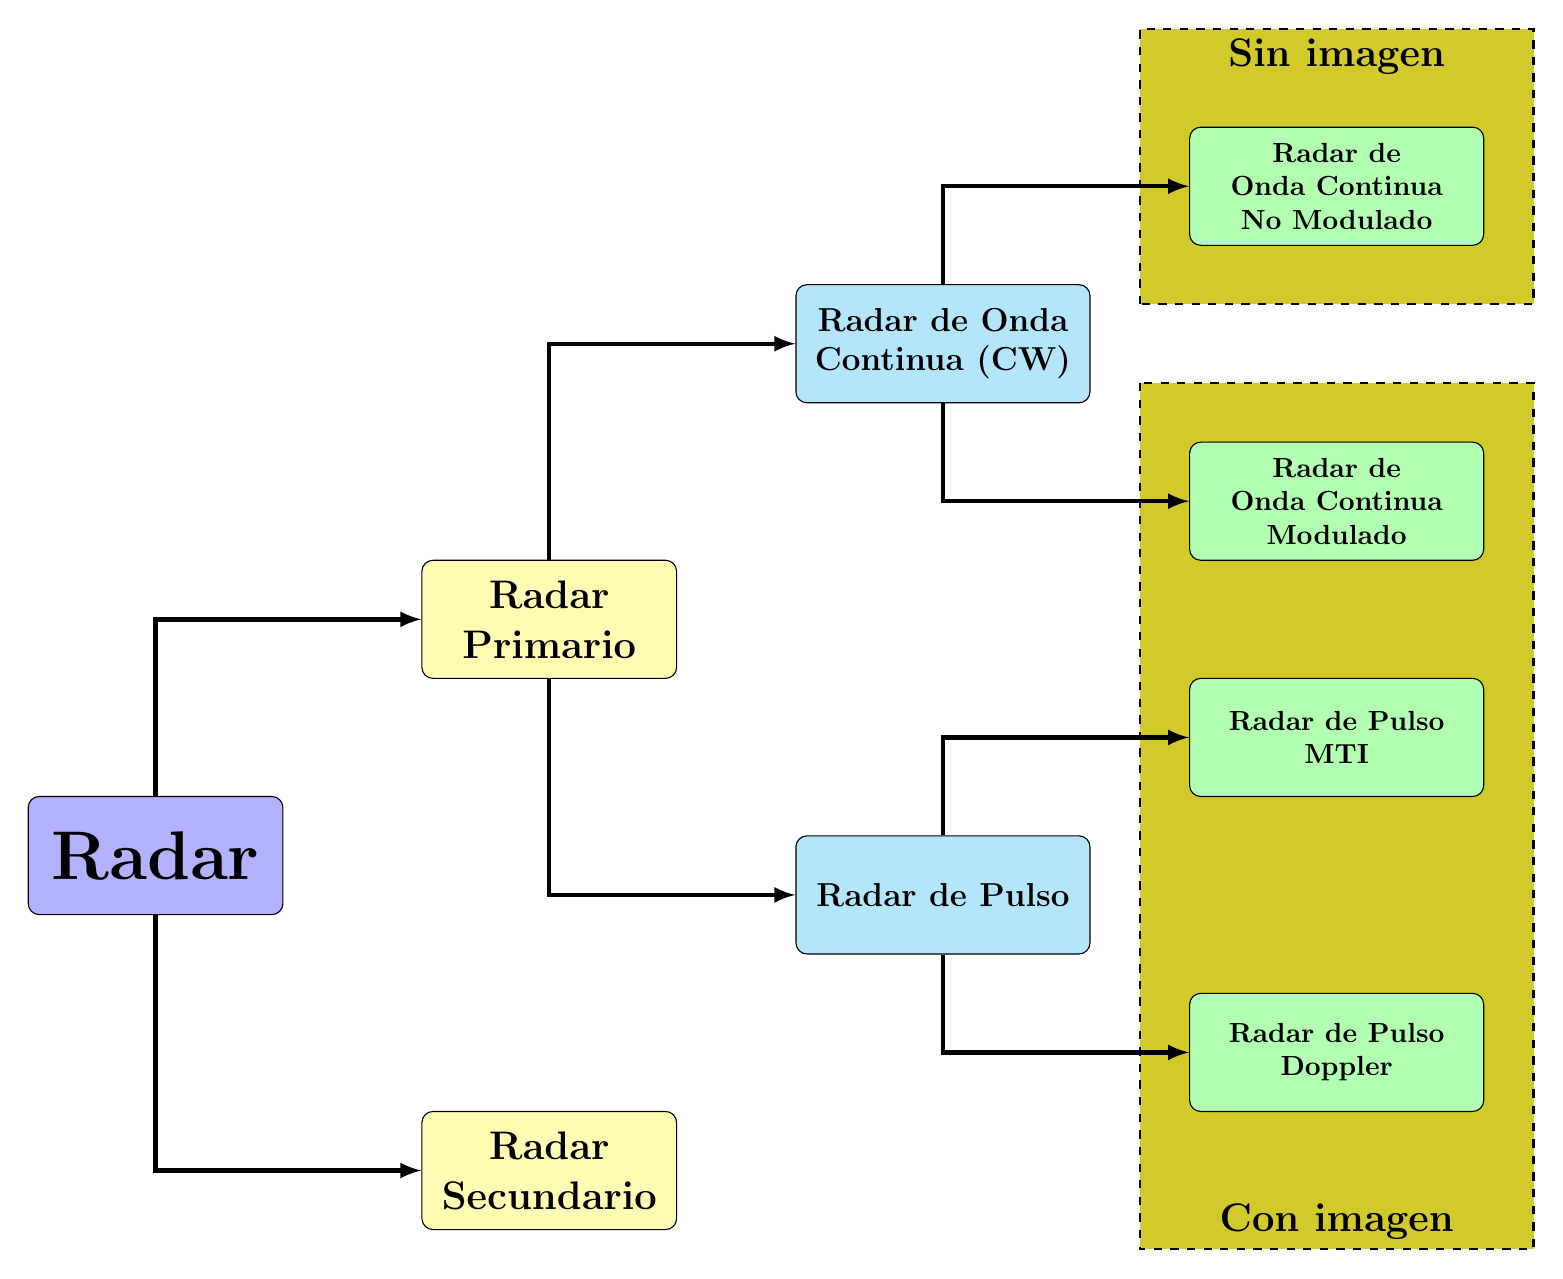
\begin{tikzpicture}[
                node distance = 2cm ,
                every node/.style={
                                       font =  \bfseries , 
                                      } ,
                  NodoPrimario/.style = {
rectangle , draw , rounded corners , 
text centered ,                                         
minimum width = 3cm ,
                                        minimum height= 1.5 cm ,
                                  text width= 3cm ,                     
                                  font = \Large \bfseries ,
                                  fill = blue!30 ,
                                    }  ,
                  NodoSecundario/.style = {
rectangle , draw , rounded corners , 
text centered ,                                         
minimum width = 3cm ,
                                        minimum height= 1.5 cm ,
                                  text width= 3cm ,                     
                                  font = \Large \bfseries ,
                                  fill = yellow!30 ,
                                    }  ,
NodoTerciario/.style = {
rectangle , draw , rounded corners , 
text centered ,                                         
minimum width = 3cm ,
                                        minimum height= 1.5 cm ,
                                  text width= 3.5 cm ,        
                                  font = \large \bfseries ,             
                                  fill = cyan!30 ,
                                  } ,
NodoCuarto/.style = {
rectangle , draw , rounded corners , 
text centered ,                                         
minimum width = 3cm ,
                                        minimum height= 1.5 cm ,
                                  text width= 3.5 cm ,  
                                  fill = green!30 ,
                                  } ,
                ]

% \draw [ green!70!black  , step = 1 cm ] ( 0 , -5 ) grid ( 20 , 10 ) ; 

\draw [ thick , dashed , fill = yellow!80!black ] ( 12.5 , 7.0 ) rectangle  ( 17.5 , 10.5 ) ; 

\node  at  ( 15.0 , 10.15 ) { \Large Sin imagen}  ;

\draw [ thick , dashed , fill = yellow!80!black ] ( 12.5 , 6.0 ) rectangle  ( 17.5 , -5 ) ; 

\node  at  ( 15.0 , -4.65 ) { \Large Con imagen}  ;

\node [ NodoPrimario ]  (radar) { \Huge Radar}  ;

\node [fill = yellow!50 , right of = radar , 
               xshift= 3 cm , yshift = 3 cm  ,                
              NodoSecundario  ] (PSR) {  Radar Primario } ; 

\node [ right of = PSR , 
               xshift= 3 cm , yshift = 3.5 cm  , 
               fill = cyan!30 , 
               NodoTerciario  ] (cw)   {Radar de Onda Continua (CW)	}   ; 

\node [ right of = cw , 
               xshift= 3 cm , yshift = 2 cm  , 
               NodoCuarto  ] (cw_NoModulado)   {Radar de \\ Onda Continua \\ No Modulado	}   ; 

\node [ right of = cw , 
               xshift= 3 cm , yshift = - 2 cm  , 
               NodoCuarto  ] (cw_Modulado)   {Radar de \\ Onda Continua \\ Modulado	}   ; 


\node [ right of = PSR , 
               xshift= 3 cm , yshift = -3.5 cm  , 
               fill = cyan!30 , 
               NodoTerciario  ] (PS)   {Radar de Pulso 	}   ; 

\node [ right of = PS , 
               xshift= 3 cm , yshift = 2 cm  , 
               NodoCuarto  ] (ps_mti)   {Radar de Pulso  \\ MTI	}   ; 

\node [ right of = PS , 
               xshift= 3 cm , yshift = - 2 cm  , 
               NodoCuarto  ] (ps_doppler)   {Radar de Pulso \\ Doppler	}   ; 



\node [fill = yellow!50 , right of = radar ,  
                                 xshift= 3 cm , yshift = -4 cm  ,
                                  NodoSecundario  ] (SSR) { \Large Radar Secundario } ; 


\draw [ ultra thick , -latex ] (radar) |- (PSR) ; 
\draw [ ultra thick , -latex ] (radar) |- (SSR) ; 

\draw [ ultra thick , -latex ] (PSR)	 |- (cw) ; 
\draw [ ultra thick , -latex ] (PSR)	 |- (PS) ; 

\draw [ ultra thick , -latex ] (cw) |- (cw_NoModulado) ; 
\draw [ ultra thick , -latex ] (cw) |- (cw_Modulado) ; 

\draw [ ultra thick , -latex ] (PS) |- (ps_mti) ; 
\draw [ ultra thick , -latex ] (PS) |- (ps_doppler) ; 

\end{tikzpicture}
}

% https://www.radartutorial.eu/02.basics/Pulse%20Radar.en.html

\begin{description}
\item[\bf Primary Surveillance Radar (PSR)]

  Los equipos de radar primario emiten señales de alta frecuencia que se reflejan en los objetivos. A diferencia de los radares secundarios , los radares primarios reciben sus propias señales emitidas en forma de ecos. Las señales de eco resultantes se reciben y evalúan.


  % transmite una señal electromagnética hacia un objeto, p.e. una aeronave, que actúa como elemento pasivo y refleja esta señal hacia el emisor.

  % El PSR permite detectar no sólo aeronaves con transpondedores funcionando y respondiendo, sino también aeronaves sin transpondedores operativos y otros objetos
  % que no son aeronaves pero que pueden ser potencialmente de interés.
  % Para maximizar la cantidad de espacio aéreo cubierto por barrido de 360º, el haz de radar de la mayoría de los transmisores PSR civiles tiene forma de abanico.
  % En un momento dado el haz cubre (para todos los efectos) solo un acimut pero se distribuye en una amplia gama de ángulos de elevación.
  % El radar no tiene forma de determinar el ángulo de elevación de una señal reflejada que regresa, por lo que es difícil que pueda determinar la altitud del objeto,
  % introduciendo cierta imprecisión y una cantidad variable de inexactitud  en la posición terrestre de un objetivo, puesto que el objeto que produce el retorno podría estar ubicado
  % en cualquier lugar a lo largo de un segmento de arco vertical   a la distancia inclinada del objetivo en el plano del haz del radar.
  
  % Ejemplo de PSR:   Air Traffic Control (ATC) radar.

\item[\bf Secondary Surveillance Radar (SSR)] transmite una señal electromagnética hacia una aeronave, que actúa como elemento activo y responde con la misma señal devuelta al radar secundario.
  Ejemplo de SSR: el transponder a bordo de la aeronave. El transponder responde a la interrogación transmitiendo la respuesta al código en la señal devuelta, conteniendo información como altitud, identificación,  etc.

\item [\bf Radar de onda continua]  o radar CW irradia una potencia de transmisión sin interrupción. La señal de eco se recibe y procesa de forma simultánea y continua. El receptor no tiene por qué estar necesariamente en el mismo lugar que el transmisor. Cualquier transmisor de radiodifusión potente también puede funcionar como transmisor de radar si un receptor remoto compara los tiempos de propagación de la señal directa con la señal reflejada. La ubicación exacta de un avión se puede calcular evaluando las señales de tres estaciones de televisión diferentes.

  
\item[\bf Radar de Pulso] emiten una señal pulsada (encendido/apagado) de alta potencia y muy alta frecuencia. A esto le sigue una pausa más larga durante la cual se pueden recibir los ecos antes de transmitir una nueva señal de transmisión. La distancia direccional y, en caso necesario, la altura del objetivo se pueden determinar a partir de la posición de la antena y la duración de la señal.

\item [\bf  Radar CW no modulado]
La señal transmitida de estos dispositivos es constante en amplitud y frecuencia. Estos dispositivos están especializados en mediciones de velocidad y hacen uso de la frecuencia Doppler. Las distancias no se pueden medir. La policía los utiliza, por ejemplo, como medidores de velocidad .

 
\item [\bf Radar de onda continua modulada en frecuencia (FMCW-Radar)] 
  La señal transmitida es constante en amplitud pero modulada en frecuencia, o en cambio de fase . Esto permite determinar la distancia según el principio de medición del tiempo de ejecución. La distancia (o altura) puede entonces determinarse a partir del cambio de frecuencia o por el tiempo de retardo de un código de fase determinado. La ventaja de estos equipos de radar es que la evaluación se realiza sin tiempo de espera para la recepción y, por tanto, el resultado de la medición está disponible continuamente.
  
% \item [\bf Radares modulados por intrapulso]
% Estos equipos de radar transmiten con menor potencia de pulso pero con mayor duración de pulso. Modulan su pulso transmitido (similar al radar FMCW) para utilizar la compresión del pulso para determinar la distancia incluso dentro de la duración del pulso transmitido.

% \item[\bf Conjuntos de radar biestáticos]
%   Un radar biestático consta de dos o más sitios de transmisión y recepción separados por una distancia considerable.

  
\item[\bf Radar de pulso Doppler] capaz no solo de medir el rumbo, distancia y altitud de un objeto, sino también de detectar su velocidad. Su sistema de localización se basa en emitir trenes de pulsos a una frecuencia determinada y utilizar el efecto Doppler para determinar la velocidad transversal relativa de los objetos. Este tipo de radares presentan ambigüedad en la medida de distancias por lo que no son muy útiles para labores de localización. 

  
\end{description}

\href{https://www.gacetaeronautica.com/gaceta/wp-101/?p=22386}{Radares Argentinos.}


\begin{table}[!h]
  \centering
  \begin{tabular}{m{0.24\textwidth}m{0.6\textwidth}} \hline \rowcolor{cyan!30}
   \textbf{Tipos de radares} & \textbf{	Función} \\ \hline
Radar de defensa aérea &	Determina la ubicación del objetivo y lanza el arma para destruir la amenaza. \\ \rowcolor{cyan!15}
Radar aéreo 	& Para la navegación, principalmente para operaciones aéreas. Guía a los aviones incluso en nubes espesas. También se utiliza para aplicaciones militares. \\
Radares de tráfico aéreo &	Determina la ubicación del aterrizaje de aviones en el aeropuerto. Ayuda a los aviones a aterrizar en condiciones climáticas adversas y de mala visibilidad. \\  \rowcolor{cyan!15}
Radar policial &	Localiza y determina vehículos que se mueven rápidamente. \\
Radar marino 	& Determina la ubicación de la costa y los barcos. \\  \rowcolor{cyan!15}
Radar terrestre &	Este radar crea un mapa de radar del terreno desde un satélite o un avión. \\
Guía de misiles &	Controla la trayectoria del misil lanzado desde el suelo hacia el objetivo. \\ \rowcolor{cyan!15}
Radar meteorológico &	Este radar meteorológico pronostica las condiciones meteorológicas antes de despegar del avión. \\
Radar de atraque &	Guíe los vehículos a la posición de atraque correcta. \\ \rowcolor{cyan!15}
    Radar de orientación del terreno  &	Ayuda a guiar la aeronave durante el vuelo sobre montañas y terrenos a lo largo de la ruta. \\
    Radioaltímetro & Indica la altura de vuelo de una aeronave \\ \hline
    \\ \hline
  \end{tabular}
  \caption{Radares según la función que cumplen}
  \label{tab:06.Radar.segunFuncion}
\end{table}


\subsection{Radio-alt\'imetro}
\label{sec:U06.05.radio.altimetro}

El radioalt\'imetro (Radio Altimeter) utiliza transmisiones de radar para reflejarse en la superficie del mar o el suelo inmediatamente debajo de la aeronave. Por lo tanto, el radioalt\'imetro proporciona una lectura absoluta de altitud con respecto al terreno directamente debajo de la aeronave. Esto contrasta con el altímetro barométrico o de datos aéreos donde la altitud puede ser referenciada al nivel del mar o algún otro dato como el terreno local, donde se conoce como altura. Por lo tanto, el radioalt\'imetro tiene un valor particular para advertir al piloto que está cerca del terreno y para advertirle si es necesario que tome medidas correctivas. Alternativamente, el radioalt\'imetro puede proporcionar a la tripulación de vuelo una altitud precisa con respecto al terreno durante las etapas finales de una aproximación de precisión. La comparación de la altitud barométrica y de radar se muestra en la Figura \ref{fig:radioaltimetro.funcionamiento}. \textbf{Debe advertirse que el radioalt\'imetro NO INDICA LA ALTURA POR DELANTE DE LA AERONAVE}.

Estos equipos llevan varios a\~nos emple\'andose en la aeronaves, como ejemplo puede verse en el siguiente hiperv\'inculo un art\'iculo de 1939: 
\href{https://www.rfcafe.com/references/radio-craft/radio-altimeter-increases-air-safety-january-1939-radio-craft.htm}{New Radio Altimeter Increases Air Safety
January 1939 Radio-Craft}. 

\begin{figure}[!h]
  \centering
    \includegraphics[width=0.85\textwidth]{06.radionavegacion/Imagenes/06.05.radar/06_radar_0000.png}
  \caption{Radioalt\'imetro. Altura medida por radar $h$ y altura barom\'etrica.. \\{\tiny Adaptado de \,\url{https://www.naic.edu/~phil/rfi/NAR_Radio_Altimeter.pdf}}}
  \label{fig:radioaltimetro.funcionamiento}
\end{figure}


Los radioalt\'imetros pueden operar usando CW/FM (onda continua / frecuencia modulada) o técnicas de señal pulsada. Las técnicas CW/FM pierden precisión por encima de un rango de 2500 pies (762 m) por arriba del terreno \ac{AGL}, por lo que muchos radioaltímetros están limitados a un rango operativo hasta esta altura. Por encima de esto, se deben utilizar técnicas pulsadas. El principio de funcionamiento del altímetro radar se muestra en la Figura \ref{fig:radioaltimetro.principio.funcionamiento}. 

El oscilador y el modulador proporcionan las señales necesarias para el transmisor y las antenas de transmisión, que dirigen la energía del radar hacia el terreno debajo de la aeronave con un ancho entre 20º a 40º. 
Las antenas de recepci\'on reciben la se\~nal reflejada y la pasan a un contador de frecuencia, el cual demodula la señal recibida y proporciona una lectura del radioalt\'imetro a una pantalla dedicada.


\begin{figure}[!htb]
  \centering
  \subfigure[Principio de funcionamiento del radioalt\'imetro. Adaptado de \protect\cite{Moir_Civil_Avionics_Systems}]{        \includegraphics[width=0.45\textwidth]{06.radionavegacion/Imagenes/06.05.radar/06_radioaltimetro_principio.png}
  \label{fig:radioaltimetro.principio.funcionamiento}}
  \hspace{0.05\textwidth}
  \subfigure[T\'ecnica de modulaci\'on de frecuencia en radioalt\'imetro. Adaptado de \protect\cite{Moir_Civil_Avionics_Systems}]{  \includegraphics[width=0.45\textwidth]{06.radionavegacion/Imagenes/06.05.radar/06_radar_0002.png}
  \label{fig:radioaltimetro.tecnica.modulacion.en.frecuencia}
	}
    
\end{figure}


La mayoría de los radioalt\'imetros utilizan una técnica de frecuencia modulada triangular en la energía transmitida, como se muestra en la Figura \ref{fig:radioaltimetro.tecnica.modulacion.en.frecuencia}, aunque como se mencionó anteriormente, esto típicamente limita el rango operativo a 2500 pies (762 m). El transmisor / receptor genera una señal de onda continua (CW) que varía de 4250 a 4350 MHz, modulada a 100 Hz (período $\mu 0.01$ seg). La comparación de la frecuencia de la energía reflejada con la energía transmitida: $f_1$ versus $f_2$, en la mencionada Figura  arroja una diferencia de frecuencia que es proporcional al tiempo que tarda la energía radiada en regresar, por lo tanto, se puede calcular la altitud.

% \begin{figure}[!htb]
%   \centering
%   \includegraphics[width=0.5\textwidth]{06.radionavegacion/Imagenes/06.05.radar/06_radar_0002.png}
%   \caption{T\'ecnica de modulaci\'on de frecuencia en radioalt\'imetro. Adaptado de \protect\cite{Moir_Civil_Avionics_Systems}}
%   \label{fig:radioaltimetro.tecnica.modulacion.en.frecuencia}
% \end{figure}

En la Figura \ref{fig:radioaltimetro.indicador} 
se muestra un indicador de radioalt\'imetro t\'ipico donde se han indicado sus partes, puede apreciarse que la escala es lineal entre cero y 500 pies y luego es logar\'itmica hasta los 2500 pies.

\begin{figure}[!htb]
  \centering
  \includegraphics[width=0.5\textwidth]{06.radionavegacion/Imagenes/06.05.radar/06_radar_0004.png}
  \caption{Indicador de radioal\'imetro}
  \label{fig:radioaltimetro.indicador}
\end{figure}


Las instalaciones de radioalt\'imetro se calibran seg\'un su instalación en la aeronave, esto permite compensar la altura de la antena sobre el tren de aterrizaje y cualquier largo recorrido de cable coaxil en la instalación eléctrica de la aeronave. 
La lectura cero del altímetro del radar se establece de modo que coincida con el punto en el que el tren de aterrizaje de la aeronave está haciendo contacto con la pista. 

Una referencia útil sobre las instalaciones de radioalt\'imetro y su mantenimiento puede obtenerse en  \protect\cite{Radioaltimetro_airbus}.

Como ejemplo de un sistema de radioalt\'imetro puede consultarse el producto \href{https://www.bendixking.com/en/products/nc/navigation-and-communication/kra-405b}{KRA 405B Radar Altimeter de BendixKing} que equipa a la familia de aeronaves Embraer E2 o al helicóptero Bell 429. 

\begin{tcolorbox} {\bf \large ¡Recordar!}{ \small
    \begin{itemize}

    \item El radioalt\'imetro mide la altitud real de la aeronave en
      relación con el terreno debajo, a diferencia del altímetro
      barom\'etrico que mide la altura en relación con el nivel del
      mar o alguna otra presi\'on de referencia.

    \item La altitud del radar se determina por el tiempo necesario
      para que un pulso de radar transmitido desde el avión regrese
      reflejado desde el terreno.

    \item El tipo m\'as com\'un empleado hoy en día es el de onda
      continua modulada en frecuencia (CW/FM).

    \item Los radioalt\'imetros transmiten en el rango de 4250 a 4350
      MHz.

    \item Los radioalt\'imetros pueden tener pantallas dedicadas; los
      últimos sistemas muestran la altitud del radar en el EFIS.

    \item Las aeronaves militares y UAV también pueden usar altímetros
      láser.

    \item La información puede presentarse en un EFIS. En los sistemas
      actuales la altitud del radar se proporcionará a una gama de
      sistemas como FMS, EGPWS, piloto automático, etc., y se mostrará
      directamente a la tripulación de vuelo.
 
    \item Los radioalt\'imetros generalmente operan en un rango máximo
      de cero a 2500 pies (762 m).

    \end{itemize}
}
  \end{tcolorbox}



 \subsection{Radar meteorol\'ogico}
 \label{sec:U06.06.radar.metereologico}

 Existen tres tecnologías principales que se usan típicamente en las aeronaves para detectar las condiciones climáticas:

\begin{itemize}
     \item Radar a bordo,
     \item Detección de rel\'ampagos y
     \item Servicios de enlace de datos (Datalink services).
\end{itemize}

 El radar meteorológico ha estado en uso desde hace varios años para alertar a la tripulación de vuelo sobre la presencia de condiciones climáticas adversas en la ruta de vuelo de la aeronave y obst\'aculos sobre el terreno. 

 La mayoría de las aeronaves de transporte comercial están equipadas con radar meteorológico, y esto representa la mayoría de este capítulo. Las aeronaves de aviación general que no están equipadas con radar suelen estar equipadas con una tecnología alternativa, es decir, detección de rel\'ampagos y/o servicios de enlace de datos.
 Este se utiliza para  detectar la energía reflejada por el contenido de una nube, o por precipitación. Esta precipitación puede ocurrir en muchas formas diferentes, incluyendo: lluvia, lluvia helada, nieve, aguanieve y granizo. 

 El radar meteorológico irradia energía en un haz estrecho, con un ancho de haz de $\sim 3$º que puede reflejarse en las nubes o en el terreno por delante de la aeronave, escaneando a ambos lados de la línea central de la misma a fin de obtener  una imagen de los objetos que puedieran encontrarse. La antena también puede inclinarse en elevación alrededor de $\pm 15$º desde la horizontal para escanear áreas por arriba y por debajo de la aeronave.

El principio de funcionamiento de este equipo se muestra en la 
Figura 8.33. Se presenta en la misma una nube de tormenta directamente delante de la aeronave, con algo de precipitación por debajo y también terreno en constante aumento. La precipitación puede indicar  una probable corriente vertical de viento peligrosa para la aeronave.

 El radar meteorológico funciona en la Banda C (4 a 8 GHz) o en la banda X (8 a 12,5 GHz), 
ver Tabla \ref{tab:06.bandas.radar}. 
Estas dos bandas tienen sus ventajas y desventajas para su uso en aplicaciones de radar meteorológico:


% Airbus Optimum use of weather radar
%https://safetyfirst.airbus.com/app/themes/mh_newsdesk/pdf.php?p=25835

% \begin{itemize}
% \item Los pulsos de energía de microondas de Banda C pueden penetrar a
%   través de fuertes precipitaciones, proporcionando así la detección
%   del clima, permitiendo al piloto determinar más detalles del patrón
%   del clima.
% \item Los pulsos de energía de microondas de Banda X pueden proporcionar una buena resolución de imágenes; sin embargo, esto significa que solo pueden usarse para evitar el clima. Las frecuencias más altas requieren una antena más pequeña; Por esta razón, los aviones de pasajeros más grandes usan un radar de Banda X.

% \end{itemize}

% El alcance de un sistema de radar meteorológico es típicamente de 320 millas. Los pulsos de energía de microondas se reflejan en las gotas de humedad y se devuelven a la antena del radar. El sistema calcula el tiempo necesario para que los pulsos de energía sean devueltos.%; esto se muestra como una imagen en una pantalla de radar meteorológica dedicada, o la imagen se puede integrar con el sistema electrónico de visualización de vuelo. 
% % Se mide La intensidad de la energía devuelta y se emplea para determinar las dimensiones del objetivo. 
% % Un mayor contenido de humedad en una nube proporciona una mayor energía de retorno. %La antena escanea en el plano lateral para proporcionar información direccional sobre el objetivo.
% la imagen del radar generalmente se muestra en una pantalla de radar dedicada o se superpone en la pantalla de navegación del piloto o primer oficial. Las pantallas son típicamente en color, lo que ayuda a la tripulación de vuelo a interpretar los datos del radar. Las pantallas tienen varios marcadores de rango seleccionables y generalmente se refieren al rumbo de la aeronave. Se pueden proporcionar pantallas separadas para el clima o los modos de turbulencia. 

% \Video{
%   En el siguiente hiperv\'inculo se puede apreciar un
%   \href{https://www.youtube.com/watch?time_continue=27&v=cWD-dIrhObE&feature=emb_logo}{video
%     de funcionamiento de un radar metereol\'ogico}.
% }

% El rayo del radar está directamente delante del avión con la antena en su posición media o de referencia y detectará la nube de tormenta a través de la cual el avión está a punto de volar. Al referirse a su pantalla de radar meteorológico, el piloto podrá ver si las celdas de tormenta pueden evitarse alterando el rumbo hacia la izquierda o hacia la derecha. 

% El uso de la función de inclinación de la antena es crucial. 
% Si la antena está completamente elevada, la tripulación no obtendrá información completa relacionada con la precipitación de nubes de tormenta, ya que solo mirarán la parte superior de la formación de nubes. Si la antena está completamente hacia abajo, el radar detectará el terreno ascendente con preferencia a la nube de tormenta o la precipitación que se avecina. Por esta razón, muchos radares meteorológicos incorporan una función de inclinación automática para que los retornos del radar estén optimizados para la tripulación de vuelo, dependiendo de los retornos recibidos.

% La mayoría de los radares meteorológicos modernos pueden usar el procesamiento Doppler para detectar turbulencias por delante de la aeronave. Esta es una característica muy útil, ya que la cizalladura máxima del viento no necesariamente ocurre casualmente con la mayor precipitación. De hecho, algunas de las cizalladuras del viento más peligrosas pueden ocurrir en aire despejado con el avión volando en ninguna parte cerca de nubes o precipitaciones.

% \begin{itemize}
% \item Weather radar is a limited version of the mapping radar
%   optimised to detect weather as opposed to terrain

% \item The weather radar enables the flight crew to negotiate around
%   heavy weather and storm centres en-route

% \item The radar picture may be displayed upon a dedicated display –
%   most often in modern aircraft it is displayed on the navigation
%   display with aircraft navigation symbols overlaid

% \item Recently the weather radar has been used as a primary sensor to
%   aid advanced and highly accurate CNS/ATM INS/GPS [RNP = 0.3 nm]
%   approaches into challenging airports such as Juneau, Alaska
% \end{itemize}

% El sistema típico de radar meteorológico en una aeronave comprende la antena (bajo el cono de nariz),
% dos transceptores (tambi\'en bajo el cono de nariz),
% dos paneles/pantallas de control (en la cabina), ver Figura 20.2. 

% Los transceptores están ubicados en el cono de la nariz, lo que minimiza la longitud de la guía de ondas y también evita la necesidad de que la guía de ondas penetre en el mamparo de presión. 

% En una aeronave monomotora la antena puede ubicarse en el ala en una cápsula autónoma, ver Figura 20.3 

% \begin{description}

% \item[ \bf Antena de radar meteorol\'ogico:] Las señales del radar se transmiten y reciben a través de la antena. Las primeras versiones de esta tenían la forma de un plato parabólico, sin embargo, las versiones actuales son del tipo de placa plana, ver Figura 20.3 (a).

% La antena de placa plana proyecta un haz más enfocado que el tipo parabólico, esto se debe a la reducción de los lóbulos laterales como se observa en la 
% Figura 20.4. 
% La antena comprende una placa plana orientable con una gran cantidad de ranuras radiantes, cada una equivalente a un dipolo de media onda alimentado en fase. 
% La antena está montada en el mamparo de presión hacia adelante detrás del radomo,
% la cual es una pieza de estructura aerodinámica construida con materiales que tienen baja atenuación de las señales de radar (kevlar).

% La condición mecánica del radomo es muy importante para la efectividad del sistema de radar meteorológico, p.e. la delaminación afectar\'a la atenuaci\'on de la se\~nal.

% La antena se mueve automáticamente desde su izquierda a su derecha de forma repetitiva para poder escanear los patrones climáticos por delante del avión. Para investigar las formaciones de nubes, el piloto también puede inclinar la antena hacia arriba o hacia abajo para proporcionar diferentes perspectivas de visualización.

% La posición de referencia es escanear la antena para proporcionar imágenes a través del horizonte; las entradas del sistema de referencia de actitud de la aeronave se utilizan para proporcionar la estabilización.

% Los motores se utilizan como parte de un mecanismo de accionamiento para atravesar la antena en acimut y para inclinar la antena en tono. Los transmisores sincronizados se utilizan para retransmitir las diversas posiciones de la antena de vuelta al transceptor.

% Los pulsos de energía se transportan entre la antena y el transceptor a través de una guía de ondas, 
% ver Figura 20.3.
% Esto se debe a que las pérdidas en un cable coaxial serían altas en frecuencias superiores a 3 GHz y prohibitivas en frecuencias superiores a 10 GHz. Los cables coaxiales también están limitados en términos de la capacidad máxima de manejo de potencia. Las guías de onda tienen sus desventajas. Son voluminosas, caras y requieren más mantenimiento. Fabricadas en aleación de aluminio, en forma rectangular hueca, tienen dimensiones muy parecidas a la longitud de onda del sistema. %El Capítulo 2, Sección 2.12 proporciona más detalles sobre las guías de onda.

% \Alerta{      La energía radiada por un sistema de radar meteorológico es
%       peligrosa y puede causar da\~nos a la salud.
% }

% \item[\bf Transceptores:] El transceptor es un transmisor y receptor combinados, Figura 20.5; la potencia de salida de la antena es del orden de 5 a 10 kW. Los transceptores modernos son dispositivos de estado sólido, que incorporan procesamiento de video para la pantalla y señales de estabilización para la antena. Dado que la energía recibida de un tamaño dado de gota de agua varía con el rango, los retornos de energía de los rangos más cercanos serán más altos que los recibidos de las gotas más alejadas. El transceptor compensará automáticamente los retornos de objetivos que están cerca o lejos del avión. Esto se logra al alterar la ganancia en función del tiempo desde que se transmite el pulso de energía. Pulsos de energía de radar se transmiten de forma repetitiva; el intervalo entre pulsos depende del rango seleccionado por la tripulación. Debe dejarse tiempo para que el pulso de energía se refleje de las gotas de agua en el límite del rango seleccionado antes de que se transmita el siguiente pulso.

% \item[\bf Panel de control:]  En las Figuras 20.6 (a) y (b) se muestra un panel de control de radar meteorológico típico. Esto permite al piloto seleccionar el transceptor izquierdo o derecho, seleccionar el modo de radar meteorológico, inclinar manualmente la antena y seleccionar la ganancia del sistema.

% \item[\bf Pantalla:] La pantalla básica utilizada para los sistemas de radar primario es el indicador de posición del plan (PPI). A medida que el haz se desplaza de lado a lado, una imagen radial en la pantalla (sincronizada con cada barrido) se mueve a través de la pantalla. La imagen en la pantalla depende de la cantidad de energía devuelta desde el objetivo. Los sistemas de radar meteorológicos originales tenían pantallas monocromáticas dedicadas basadas en un tubo de rayos catódicos (CRT); Estos han evolucionado a lo largo de los años en pantallas a todo color, a menudo integradas con otros instrumentos electrónicos de vuelo. Los beneficios completos de un sistema de radar meteorológico se pueden apreciar cuando el sistema se utiliza en una aeronave con una pantalla de sistema electrónico de instrumentos de vuelo (EFIS), Figura 20.7. Se utiliza un generador de símbolos para proporcionar imágenes de radar meteorológicas específicas según lo determine el transceptor. Un panel de control con pantalla electrónica permite a cada piloto seleccionar el alcance del radar meteorológico en incrementos de 10, 20, 40, 80, 160 y 320 millas.

% La pantalla electrónica se superpone al modo de mapa, lo que permite al piloto relacionar el rumbo del avión con las imágenes meteorológicas. Estas imágenes están codificadas por colores para permitir al piloto evaluar la gravedad de las condiciones climáticas. Los colores (que van del negro, verde, amarillo, rojo y magenta) se utilizan para indicar las tasas de lluvia que pueden interpretarse como un nivel de turbulencia.



% \end{description}







% Se puede encontrar información útil sobre el uso operativo del radar meteorológico en la Referencia [13], que proporciona una guía piloto para la operación del radar meteorológico Honeywell RDR-4B. El transmisor funciona a 9345 GHz y el sistema tiene tres modos básicos de operación:

% \begin{itemize}
% \item clima y mapa con un rango maximo de 320 nm;

% \item modo turbulencia (TURB) a 40 nm;

% \item detección de cizalladura del viento a 5 nm.
% \end{itemize}

% Los radares meteorológicos también pueden usarse en un modo de evitación del terreno en ciertas circunstancias, como se muestra en la Figura 8.34. Cuando el vuelo de precisión se aproxima a aeródromos rodeados de terreno elevado, el radar meteorológico puede proporcionar una verificación cruzada independiente de la información proporcionada por el Sistema de advertencia de evitación del terreno (TAWS). El capitán puede ver la información de TAWS en su pantalla de navegación (ND) mientras es monitoreado por el primer oficial con una pantalla meteorológica superpuesta en su ND. En la Referencia [14], el texto explica por qué se agregó el radar meteorológico a la lista de equipo mínimo (MEL) de la aeronave para dichos vuelos.

% Como ejemplo de readares metereol\'ogicos comerciales se tiene el \href{https://www.bendixking.com/content/dam/bendixking/en/documents/downloads/006-08755-0001_3-rdr-200-pilot-guide.pdf}{BendixKing RDR 2000 que presenta un manual para pilotos} y tambi\'en ofrecen \href{https://www.bendixking.com/en/products/ttw/terrain-traffic-weather/rdr-2000}{videos explicativos}, o el sistema \href{https://www.garmin.com/en-US/blog/wp-content/uploads/2006/08/flyingMag.pdf}{Garmin GWX 68}. Dichos ejemplos pueden ser consultados en sus hiperv\'inculos.



% \begin{itemize}
% \item El radar de mapeo utiliza un haz especialmente diseñado para   ``pintar'' el terreno delante del avión

% \item Un mapa detallado del radar del terreno y otras funciones hechas   por el hombre delante del avión puede ser compilado

% \item Al colocar la antena de radar de mapeo en un angulo fijo de   depresi\'on, cierto grado de se puede proporcionar orientación para   evitar el terreno

% \item Los radares de mapeo se usan con mayor frecuencia en aviones   militares como parte de la suite de armas ofensivas

% \item Los radares de mapeo se utilizan en aeronaves civiles para   ilustrar el terreno en un modo de evasión del terreno

%   Figura 8.34 Uso del radar meteorológico en modo mapeo / evitación   del terreno
% \end{itemize}


% \subsection{\ac{TAWS}}
% \label{sec:06.taws}

% Este sistema 



% \Informacion{Situación al 2012 de la cobertura de los Sistemas de Navegación Aérea en la Republica Argentina}{
% En el \href{http://sedici.unlp.edu.ar/bitstream/handle/10915/37756/Resumen.pdf?sequence=1&isAllowed=y}{siguiente link} se  puede acceder a este informe realizado por el 
% GTA -  Grupo Transporte Aéreo  de la UID ``GTA-GIAI'', Departamento de Aeronáutica, Facultad de Ingeniería, Universidad Nacional de La Plata.
% }


% \Informacion{Manual de radioayudas a la navegaci\'on a\'erea}{
% La ANAC dispone 
% \href{https://www.anac.gov.ar/anac/web/uploads/navegacion/navegacion/manual-de-radioayudas-2012.pdf}{del siguiente manual versi\'on 2012.}
% }

% Capítulo 7. Directores y control automático de vuelo
% 7.1      Indicador director de actitud, Indicador de situación horizontal.
% 7.2      Componentes y modos del director de vuelo, diagrama en bloque, flujo de señales.
% 7.3      Piloto automático, componentes, diagrama en bloque, funcionamiento en los distintos modos.


\chapter{Directores y control autom\'atico de vuelo}
\label{chap:U07.director.vuelo}

\section{Introducci\'on}
\label{sec:07.00.introduccion}

Estos sistemas tienen como finalidad guiar al piloto para que \'este efect\'ue en forma correcta las maniobras de vuelo seg\'un el modo de operaci\'on elegido, adem\'as cumple las funciones b\'asicas de indicaci\'on de actitud y rumbo.

En esencia un Director de Vuelo, en ingl\'es \ac{FDS}, es un sistema de Piloto Autom\'atico sin los servos. El sistema efect\'ua los mismos c\'alculos y sensados que el Piloto Autom\'atico pero es el Piloto Humano quien controla la aeronave y realiza las maniobras siguiendo las instrucciones del panel de control. Varios sistemas de Piloto Autom\'atico disponen la posibilidad de acoplar o desacoplar al \ac{FDS}.

Existen diferentes tipos de \ac{FDS} en cuanto a la forma de 
indicaci\'on y selecci\'on de modos pero cumplen la misma funci\'on. Para la descripci\'on de un sistema t\'ipico se emplear\'a el provisto por la empresa Sperry el Sperry Three Axis Attitude Reference System (STARS), desarrollado en los a\~nos 1960. Se lo suele encontrar en aviones comerciales y particulares donde se integran con los Pilotos Autom\'aticos.


\section{Componentes de cabina}
\label{sec:componentes.cabina}

Un \ac{FDS} puede emplear una o dos pantallas, o estar integrada a otro sistema de presentaci\'on de datos. 
La primera presenta un conjunto de barras de comando, una horizontal y otra vertical. Las barras de comando en esta configuración se mantienen en una posición centrada. 
La segunda emplea un avión en miniatura alineado a una señal de comando.

\begin{figure}[!h]
  \centering
    \includegraphics[width=0.75\textwidth]{07.directores.y.ctrol.automatico.vuelo/imagenes/adi+hsi+computador_presentacion.png}  
  \caption{Componentes t\'ipicos de un \ac{FDS}. Arriba a la izquierda el ADI, abajo a la izquierda el HSI, abajo a la derecha la Computadora de Control. (Gentileza Sperry) }
  \label{fig:07.componentes.tipico.FDS.sperry-STARS}
\end{figure}


\subsection{Indicador y Director de Actitud }
\label{sec:adi}

El \ac{ADI} 
 posee una esfera indicadora de actitud y punteros de 
mando (lateral y vertical), que dan al piloto la informaci\'on requerida
para interceptor y mantener una determinada senda de vuelo que, junto
con sus dem\'as componentes, son:

\begin{figure}[!h]\centering
  \includegraphics[width=0.98\textwidth]{07.directores.y.ctrol.automatico.vuelo/imagenes/adi.png}
  \caption{Imagen de ADI (gentileza Sperry)}
\label{fig:07.adi.sperry}
\end{figure}

\begin{itemize}
	\item {\bf Esfera de actitud: } parte m\'ovil donde est\'a simbolizado
	el horizonte terrestre, sus movimientos con respecto a un avi\'on simb\'olico
	fijo, indican la actitud en alabeo y cabeceo de la aeronave.

        \item {\bf Avi\'on simb\'olico en miniatura: } s\'imbolo fijo al centro del
	instrumento y con respecto a su centro dan su indicaci\'on las barras de mando, 
	adem\'as de cumplir la funci\'on indicada en el punto anterior.

        \item {\bf Indice de actitud en alabeo: } se mueve con la esfera indicando
	exactamente las gradas en esta actitud.

        \item {\bf Barras de mando: } su funci\'on es dirigir al piloto para interceptar
	y mantener una predeterminada senda de vuelo con la condici\'on de ``volar''
	el peque\~no avi\'on simb\'olico hacia las barras de comando y tratar de
	mantener el centro de este en la intersecci\'on de las barras.
	La barra de mando vertical comanda las actitudes a tomar en alabeo y la
	horizontal en cabeceo.
	Dado que el ``avi\'on'' es fijo, al tomar la actitud correcta las barras que
	son m\'oviles se posicionar\'an en el centro de este s\'imbolo.

        \item {\bf Escala de senda de planeo: }
	el \'indice muestra la desviaci\'on del avi\'on del centro del haz de senda de 
	planeo (Glide Slope) cuando es sintonizada la frecuencia del ILS y la se\~nal
	recibida es v\'alida. 
	Si el avi\'on est\'a volando por debajo del haz, el \'indice se ubicar\'a
	en la parte de arriba de la escala.
	Una indicaci\'on al punto del \'indice representa, aproximadamente,
	 una desviaci\'on de 0,4º
	respecto de la l\'inea de control del haz.

        \item {\bf Barra de radio altura: }
	con el sistema de radioalt\'imetro en funcionamiento, esta barra aparece
	a la vista a los 61 m de altura respecto al terreno, movi\'endose hacia el
	avi\'on en miniatura seg\'un se desciende 

        \item {\bf Localizador expandido: }
	provee de una muy sensible indicaci\'on de la posici\'on del avi\'on
	respecto a la linea central del localizador, siendo utilizado en la
	aproximaci\'on final, dada su sensibilidad.

        \item {\bf Inclin\'ometro: }
	suministra al piloto una indicaci\'on convencional de los deslizamientos
	y derrapes del avi\'on. Al mantener la esfera indicadora centrada,
	se aseguran maniobras coordinadas.

        \item {\bf Perilla de ajuste de actitud de cabeceo: }
	permite posicionar la barra horizontal para que esta comande una
	predeterminada actitud de cabeceo durante una picada o trepada.

        \item {\bf Pulsador de prueba de actitud: }
	opera como una autoprueba del indicador de actitud. Cuando es pulsada
	la esfera se posiciona arrastrando un alabeo de 20º a la derecha
	y un cabeceo de 10º en trepada, apareciendo en este caso una bandera
	de advertencia de actitud erronea.

        \item {\bf Llave de erecci\'on r\'apida del gir\'oscopo: }
	no se encuentra sobre el instrumento, ubic\'andose en el tablero.
	Cuando esta, que es cargada a resorte, es pulsada y mantenida, 
	permite la erecci\'on del gir\'oscopo a una velocidad, aproximada,
	de 2º/minuto, cuando este gire a su m\'axima velocidad.
	Esta llave debe ser accionada cuando el avi\'on se encuentra
	nivelado, y se utiliza en caso de que el gir\'oscopo haya salido
	de su plano de referencia, como puede ocurrir por haberse tomado
	actitudes que superan las posibilidades del sistema.

\end{itemize}

\subsection{Indicador de Situaci\'on Horizontal}
\label{sec:indicador.situacion.horizontal}

El \ac{HSI} 
 provee adem\'as de la indicaci\'on de rumbo del avi\'on
una indicaci\'on pictogr\'afica que representa la posici\'on
de la aeronave respecto a un localizador VOR, y una indicaci\'on de la
posici\'on del avi\'on respecto a la senda de planeo.

\begin{figure}[!h]
  \centering
  \includegraphics[width=0.98\textwidth]{07.directores.y.ctrol.automatico.vuelo/imagenes/hsi.png}  
  \caption{Imagen HSI (gentileza Sperry)}
  \label{fig:07.hsi.sperry}
\end{figure}


La descripci\'on de cada uno de sus componentes:

\begin{itemize}
	\item {\bf S\'imbolo del avi\'on:} se encuentra fijo e indica la
		posici\'on de la aeronave respecto a un curso de radio
		y a un cuadrante m\'ovil indicador del rumbo. Esta fijado
		al vidrio del instrumento.

        \item {\bf Cuadrante rotante de rumbo:} provee ula informaci\'on de un
	comp\'as magn\'etico girosc\'opico, girando seg\'un los rumbos tomados por
	la aeronave a trav\'es de los 360º.

        \item {\bf Indice principal de rumbo: } 
	es fijo y marca sobre el cuadrante el rumbo del avi\'on.

        \item {\bf Marcas de azimut: }
	se encuentran fijas a una diferencia de 45º a trav\'es de los 360º

        \item {\bf Indice y perilla de rumbo selectado: }
	por medio de la perilla se posiciona el \'indice en la carta al rumbo
	deseado. La diferencia angular entre el rumbo del avi\'on y el preselectado
	

        \item {\bf Puntero y perilla de curso: } este se osiciona en el cuadrante de 
	rumbo por medio de la perilla de curso de manera que
	coincida con el radial de VOR o curso de localizador deseado.
	Igual que el \'incide de rumbo selectado, el puntero de curso es posicionado
	sin afectar la indicaci\'on del cuadrante de rumbo, pero al girar este
	lo hace de igual forma.
	El puntero provee en forma continua la informaci\'on del error de curso
	al piloto y a la computadora del sistema, de manera que 
	cuando es selectado un modo de radio, la barra vertical en el ADI
	dirije al piloto para que controle los comandos y asuma las actitudes
	de alabeo que lo llevar\'an a interceptar y mantener el curso de radio
	selectado, todo esto con la condici\'on de matener la barra vertical en el 
	ADI centralizada.

      \item {\bf Barra de desviaci\'on de curso: }
	representa la l\'inea central del curso selectado de VOR o localizador, 
	el s\'imbolo del avi\'on muestra la posici\'on relativa del mismo
	respecto al curso selectado. Esta barra se mueve paralelamente al puntero
	de curso seg\'un la se\~nal de radio recibida.

      \item {\bf Puntos de desviaci\'on de curso: }
	en la operaci\'on de VOR, cada punto representa 5º de desviaci\'on de la l\'inea
	central y en ILS, es 1º.

      \item {\bf Indicador de ``\emph{hacia-de}'': }
	son dos banderas que aparecen, una por vez e indicando si se est\'a alejando
	de la estaci\'on ``\emph{de}'' o si se va hacia ella ``\emph{hacia}''.

      \item {\bf Disco m\'ovil de curso: }
	es el sost\'en f\'isico del puntero de curso, barra de desviaci\'on de curso,
	indicador de ``\emph{hacia-de}'', y puntos de desviaci\'on de curso.
	Este disco gira por medio de la perilla de curso, arrastrando los elementos
	sostenidos en \'el. Est\'a pintado de manera que se confunde con el
	cuadrante de rumbo, dado que no es un elemento indicador.

      \item {\bf \'Indice y puntos de desviaci\'on de senda de planeo: }
	repite la informaci\'on de desviaci\'on de senda de planeo dada por el ADI.
	El \'indice se muestra al sintonizar una frecuencia de localizador.
	Cuando el avi\'on se encuentra por debajo de la senda de planeo, 
	el \'indice se encuentra en la parte de arriba de la escala.
	Cada punto representa $0.4$º de desplazamiento.

      \item {\bf Anunciador de sincronismo:}
	es una marca de punto (.) o cruz (x) que aparece en una peque\~na ventanilla
	indicando el sentido del error del rumbo indicado por el cuadrante de
	rumbo respecto al verdadero rumbo magn\'etico del avi\'on.
	Cuando el rumbo indicado es el verdadero las marcas de punto y cruz
	aparecer\'an alternativamente en la ventanilla indicando el sincronismo
	entre el cuadrante de rumbo y el sistema girosc\'opico autocorregido.

      \item {\bf Llave de ``\emph{esclavo - libre}'': }
	no se encuentra en el HSI, siendo ubicada en un lugar conveniente en el tablero
	y se selecta por medio de ella el modo de trabajo del comp\'as 
	girosc\'opico (libre o esclavizado seg\'un el rumbo magn\'etico).

      \item {\bf Llave de incremento (INC) - decremento (DEC): }
	no se encuentra 
	en el HSI, ubic\'andose cerca de la llave de   ``\emph{esclavo - libre}''.
	Con esta se posiciona el cuadrante de rumbo para obtener la
	sincronizaci\'on del sistema en el modo ``\emph{esclavo}'' y para
	modificar el rumbo indicado en el modo ``\emph{libre}''.

\end{itemize}

\subsection{Computadora de Control}
\label{sec:control.computador}

Este elemento combina los datos de rumbo, actitud, altitud y receptor de 
navegaci\'on en se\~nales computadas que comandar\'an las barras
directoras del ADI.
Contiene en su frente los botones por medio de los cuales se
seleccionan el o los modos de operaci\'on deseados.

Los modos que se encuentran en operaci\'on son enunciados al iluminarse
el bot\'on correspondiente.


\begin{figure}[!h]
  \centering
  \includegraphics[width=0.6\textwidth]{07.directores.y.ctrol.automatico.vuelo/imagenes/computadora_sperry.png}  
  \caption{Imagen Computadora de Control (gentileza Sperry)}
  \label{fig:07.computadora.sperry}
\end{figure}

\section{Modos de operaci\'on}
\label{sec:modos.operacion}

Este sistema utiliza los datos de VOR-Localizadores y de Senda de Planeo,
proporcionados por los receptores de navegaci\'on corrientes.
Utiliza tambi\'en datos de altitud de un sensor de altura barom\'etrico
propio (adem\'as del de sistema de radio-alt\'imetro), datos de rumbo
desde un gir\'oscopo direccional y de actitud desde un gir\'oscopo
vertical, elementos estos que pertenecen al mismo sistema.

Todas estas informaciones son computadas siendo finalmente enviado su
resultado a comandar las barras directoras del sistema para guiar al
piloto en las maniobras que debe efectuar, para mantener o tomar la
senda de vuelo selectada, tanto para la navegaci\'on como para la
aproximaci\'on de aterrizaje.

Los modos de operaci\'on que puede selectar el piloto son los siguientes:

  \begin{tabular}{lm{3mm}llm{3mm}l}
\rowcolor{cyan!10}
    	SBY &  & Preparado &
	GO AROUND &  & Escape \\
\rowcolor{yellow!10}
	ALT &  & Mantenimiento de altura    &
	PAT &  & Ajuste de actitud en cabeceo \\
\rowcolor{cyan!10}
	HDB &  & Rumbo selectado &
	V/L &  & VOR - Localizador \\
\rowcolor{yellow!10}
        GS ARM & & Armado Pendiente de Planeo &
	GS & & Pendiente de Planeo \\
\rowcolor{cyan!10}
	GS EXT & &  &
	REV & & Curso opuesto \\
  \end{tabular}

\subsection{Modo Preparado (SBY)}
\label{sec:modo.sby}
Mediante el mismo el sistema es puesto en condiciones de operar cuando sea
requerido y encontr\'andose las barras del ADI fuera de la vista,
operando \'este como un indicador de referencia de actitud.
Este sistema est\'a energizado si lo est\'a el sistema de corriente
alterna del avi\'on, por lo tanto permite la selecci\'on de cualquier modo siempre que las banderas de precauci\'on respectivas se encuentren fuera de la
vista.

Se selecciona el moto SBY presionando la tecla correspondiente
en tablero, al seleccionarla se iluminan los dem\'as modos
como prueba de l\'amparas y al soltarlo solo SBY queda iluminado.

Al seleccionarse otro modo las barras directoras responden a las salidas
de la computadora, luego el piloto debe ``volar'' el avi\'on en miniatura
del ADI hacia las barras directoras e interceptarlas. Al mantener esta
condici\'on ser\'an efectuadas las maniobras necesarias para interceptar
y/o mantener un curso deseado.

\subsection{Modo Ajuste Actitud de Cabeceo (Pitch Attitude Trim, PAT)}
\label{sec:modo.ajuste.pitch}

Permite selectar un \'angulo de trepada o descenso por medio de la perilla
de ajuste de ajuste de actitud de cabeceo, que se encuentra en el frente y
en el extremo inferior izquierdo
del ADI (Figura \ref{fig:07.adi.sperry}, Pitch attitude trim knob).

Al presionar PAT, debe mantenerse encendida la luz de dicho modo
para que se confirme el mismo, la barra de comando de cabeceo del
ADI se ubica de manera que el piloto tome la actitud de cabeceo
deseada.

El modo PAT puede ser utilizado con cualquier otro modo de 
control de alabeo (p.e. el HDG) pero
resulta incompatible con otros modos de cabeceo (p.e. GO AROUND, ALT).

Si la se\~nal de cabeceo se torna inv\'alida, la barra de comando saldr\'a 
de vista y el bot\'on del modo permanecer\'a iluminado.

\subsection{Modo Rumbo Selectado (Heading HDG)}
\label{sec:hdg}

Se utiliza para interceptar y mantener un rumbo de vuelo deseado.
Al presionar HDG se debe iluminar el bot\'on, confirmando la
operaci\'on del mismo.
Si el modo resultara no v\'alido, la barra de comando de alabeo
saldr\'a de vista pero el bot\'on continuar\'a iluminado.

Utilizando la perilla de rumbo selectado ubicada en  el
HSI (Figura \ref{fig:07.hsi.sperry}, Heading knob),
se posiciona el \'indice de rumbo selectado en el rumbo
deseado 
(Figura \ref{fig:07.hsi.sperry}, Heading bug). 
Este debe ser menor a 170º respecto al rumbo actual de la aeronave.

La computadora controlar\'a los movimientos de la barra de
alabeo en el ADI a fin de dirigir al piloto para corregir
el alabeo del avi\'on de forma de interseptar el curso elegido
sin sobrepasamiento.

Para prevenir actitudes extremas, la computadora limita los \'angulos
de alabeo a un m\'aximo de 30º.

Si el modo HDG es selectado desde el modo SBY, en el ADI s\'olo
aparecer\'a la barra de alabeo. 
Si el modo es selectado con el modo PAT o ALT, aparecer\'a adem\'as
la barra de cabeceo.

\subsection{Modo mantenimiento de altura (ALT)}
\label{sec:alt}

Brinda la posibilidad de mantener una altura barom\'etrica deseada,
la cual ser\'a la presente al momento de selectar este modo.

Entonces, se nivela la aeronave a la altura deseada y se oprime
el modo ALT, confirm\'andose su operaci\'on por permanecer el 
bot\'on iluminado.

La computadora brindar\'a la informaci\'on necesaria para
posicionar la barra de cabeceo en el ADI, de forma de 
que el piloto tome las actitudes necesarias para mantener
la altitud barom\'etrica deseada.

Para prevenir acciones extremas, el comando del \'angulo de
cabeceo est\'a limitado a $\mp$ 10º.

En caso de alg\'un mal funcionamiento, la barra directora
de cabeceo en el ADI saldr\'a de vista y la luz de ALT
se apagar\'a en el teclado.

Adem\'as, a los efectos de proteger el elemento sensor de altura,
el modo se cancelar\'a al producirse un cambio sustancial respecto
a la altura selectada, desapareciendo la barra de control
de cabeceo.
Por ejemplo, al desviarse a nivel del mar en $\mp$ 400 pies (120 m)
o en $\mp$ 1200 pies (360 m) a 40000 pies (12000 m) de altura. 


\subsection{Modo Escape (GO AROUND)}
\label{sec:go.araund}

Este modo cancela todos los otros modos y provee un comando de trepada
prefijado, juntamente con un comando de nivelaci\'on de las alas.

El modo GO AROUND se selecta presionando el bot\'on correspondiente
sobre el teclado de la computadora o mediante un bot\'on en el
volante de mando.

En ocasi\'on de una aproximaci\'on fallida, se selecta este modo
indicando las barras del ADI la actitud a tomar.

Si el gir\'oscopo vertical asociado al sistema entrega datos
incorrectos o no v\'alidos, las barras en el ADI salen de
la vista mientras que el bot\'on GO AROUND permanecer\'a iluminado.


\subsection{Modo VOR - Localizador (V/L)}
\label{sec:V_L}

Permite mediante la barra de alabeo del ADI, interceptar y mantener
un rumbo deseado, operaci\'on que se efectuar\'a suavemente
limitando la computadora los \'angulos de alabeo a $\mp$ 30º.

\subsection{Armado Pendiente de Planeo}
\label{sec:GS.arm}

Por medio de este modo se prepara al sistema para la captura
autom\'atica del haz de pendiente de planeo 
cuando el avi\'on se aproxime al centro del haz de pendiente
de planeo desde abajo de \'este, si el avi\'on se encuentra
por arriba la luz del bot\'on GS-ARM se apagar\'a y la
computadora activar\'a autom\'aticamente el modo GS.

\subsection{Pendiente de Planeo}
\label{sec:gs}

Permite al piloto efectuar la captura de la pendiente de planeo
desde arriba o abajo del haz. La barra de mando de cabeceo mostrar\'a
la actitud a tomar, se encuentre el avi\'on arriba o abajo de la pendiente
de planeo.
La computadora limita los \'angulos de cabeceo a $\mp$ 10º aproximadamente.
La barra de mando de alabeo permitir\'a mantener la l\'inea central del
localizador.

\subsection{Modo anunciador ampliaci\'on de indicaci\'on en pendiente de planeo (GS EXT)}
\label{sec:gs.ext}

Provee un ajuste autom\'atico de ganancia para compensar el estrechamiento
del haz de pendiente de planeo, \'este modo es enganchado
autom\'aticamente al detectarse el marcador medio o a los 250 pies (76,2 m)
de altura.

\subsection{Modo Curso Opuesto (REV)}
\label{sec:rev}

Este modo da la posibilidad de volar el curso de localizador opuesto.

\section{Incorporaci\'on del sistema de radioalt\'imetro}
\label{sec:incorporacion.sistema.radio.altimetro}

El radioalt\'imetro provee una indicaci\'on de altura absoluta en un indicador,
pero adem\'as se interconecta con el director de vuelo a los fines
de manejar la barra de radioaltura en el ADI.

Cuando el sistema de radioalt\'imetro funciona, la barra de radioaltura aparece a la vista
en la parte inferior del instrumento a los 61 (sesenta y un) metros y, a medida que
el avi\'on se acerca a tierra, esta barra sube simulando el acercamiento de la aeronave
a tierra mediante el acercamiento relativo del avi\'on miniatura del ADI
a la barra en miniatura que simula el terreno.

Al tocar tierra la aeronave, la barra de altura del instrumento toca la parte
inferior del avi\'on simb\'olico del ADI.

El sistema de radioaltimetro est\'a compuesto por dos (2) antenas, una transmisora
y otra receptora, un transceptor y un indicador.
Su principio de funcionamiento se basa en la emisi\'on de ondas de UHF, moduladas
en frecuencia, por la antena transmisora, las cuales son reflejadas por la superficie
terrestre y receptadas por la segunda antena. La diferencia de frecuencia entre
las ondas emitidas y las reflejadas es representativa de la altura a la cual se
encuentra la aeronave del suelo, y es indicada en el instrumento.

En otros sistemas se utiliza la modulaci\'on de pulsos.


\section{Integraci\'on con el Sistema de Piloto Autom\'atico}
\label{sec:07.AFCS}

El \ac{AFCS} provee la integraci\'on del \ac{FDS} con el Piloto Autom\'atico, este sistema se encuentra habitualmente en aeronaves de alta performance pero debido a los avances en procesamiento digital se encuentran actualmente disponibles para aviaci\'on general.

En algunos de estos sistemas son tan avanzados que permiten extender la programaci\'on, el nivel de integraci\'on con las ayudas, integraci\'on con sistemas de control de motor y combinar todo esto en una \'unica
consola con interfaz para el usuario.

\begin{tcolorbox}

 Ejemplo de implementaci\'on de un \ac{AFCS} puede consultarse en el siguiente documento 
  \href{http://www.smartcockpit.com/docs/Bombardier_CRJ_200-Automatic_Flight_Control_System.pdf}{Canadair
    Regional Jet 100/200 - Automatic Flight Control System}.

Otro ejemplo puede encontrarse en la siguiente publicaci\'on
\href{https://static.garmincdn.com/pumac/190-00498-07_0A_Web.pdf}{Gu\'ia del piloto del sistema Garmin G1000 Integrated Flight Deck}

\end{tcolorbox}

A su vez los \ac{AFCS} pueden integrarse con los \ac{AHRS} y ayudas para la navegaci\'on incluyendo senda de planeo. 

\subsection{  Attitude and Heading Reference Systems (AHRS) }
\label{sec:07.AHRS}


Una notable mejora a los tradicionales sistemas giroscópicos vino dada por las Unidades de Medición Inercial, en ingl\'es \ac{IMU}, las cuales consisten en dispositivos que utilizando una combinación de acelerómetros y giróscopos, permiten determinar la velocidad, orientación y fuerzas gravitacionales de una aeronave.
Estas unidades constituyeron el elemento principal de los \ac{INS} empleados  en los primeros ``\emph{glass cockpits}'' en la aviaci\'on militar y comercial. Su coste era muy elevado para la aviación general por lo que  se continuaron utilizando los sistemas anteriores en esta rama.

Las \ac{IMU} presentan acumulación de errores durante su utilización,  puesto que el sistema de guiado está continuamente integrando la aceleración para calcular la velocidad y la posición, los errores de medición se acumulan (deriva).

Es aqu\'i cuando aparecen las \ac{AHRS} que brindaron un  avance notable sobre las \ac{IMU}, puesto que fueron creados para proporcionar una mayor fiabilidad y precisión. Estos sistemas consisten,  básicamente, en una serie de sensores en los tres ejes coordenados a partir de los cuales se obtiene la información de rumbo y actitud de la aeronave.
De esta forma, un AHRS proporciona al piloto orientación tridimensional mediante la integración de gir\'oscopos y la combinación de los datos obtenidos mediante acelerómetros y magnetómetros. 

Debe señalarse que los gir\'oscopos utilizados por los AHRS son muy diferentes de los tradicionales ya que, al igual que los acelerómetros y los magnetómetros, se trata de Sistemas MicroElectroMecánicos, en ingl\'es \ac{MEMS}. 

\begin{myboxAzul}{\ac{MEMS}}
 \begin{minipage}[c]{0.60\linewidth}
    Los \ac{MEMS} pueden definirse como componentes mecánicos y
    electromecánicos miniaturizados, su desarrollo comenz\'o a
    mediados de los a\~nos 1980. Para su desarrollo se utilizan
    técnicas de microfabricación similares a las empleadas en la
    producción de circuitos integrados. Estos dispositivos están
    constituidos por estructuras con tamaños típicos entre 1 y 100
    $\mu$m. En la Figura \ref{fig:07.MEMS} puede apreciarse uno de 
    estos dispositivos.

Respecto a giróscopos MEMS puede consultarse a \cite{MEMSgiroscopos}.

%Un acelerómetro piezoeléctrico utiliza el efecto piezoeléctrico (los materiales piezoeléctricos producen electricidad cuando se someten a estrés físico) para detectar cambios en la aceleración. Los acelerómetros piezoeléctricos se utilizan con mayor frecuencia en la medición de vibraciones y golpes. Los acelerómetros piezorresistentes son mucho menos sensibles que los acelerómetros piezoeléctricos y se adaptan mejor a las pruebas de choque de vehículos. Un acelerómetro de piezorresistencia aumenta su resistencia en proporción a la cantidad de presión que se le aplica. El tercer y más utilizado tipo de acelerómetro es el acelerómetro capacitivo. Los acelerómetros capacitivos utilizan cambios en la capacitancia eléctrica para determinar la aceleración de un objeto. Cuando el sensor experimenta una aceleración, la distancia entre sus placas de condensador cambia a medida que se mueve el diafragma del sensor. La mayoría de los acelerómetros son minúsculos y, a menudo, se denominan acelerómetros de sistemas microelectromecánicos (MEMS). Debido a su tamaño y asequibilidad, están integrados en una gran variedad de dispositivos electrónicos portátiles (como teléfonos, tabletas y controladores de videojuegos). En teléfonos y tabletas, el acelerómetro es responsable de 'voltear' la pantalla cuando se gira el dispositivo. Los acelerómetros también son utilizados por zoólogos (para rastrear el movimiento de animales en la naturaleza), ingenieros (especialmente en experimentos de colisión) y fábricas (para monitorear la vibración de la maquinaria).

  \end{minipage} \hspace{1em}
  \begin{minipage}[c]{0.35\linewidth}
    \includegraphics[width=\linewidth]{07.directores.y.ctrol.automatico.vuelo/imagenes/07MeMS.jpeg}
    \captionof{figure}{Un embrague microscópico fabricado con componentes MEMS \protect\cite{Miller2021Jan}}
    \label{fig:07.MEMS}
  \end{minipage}
\end{myboxAzul}


A fin de tener en cuenta la deriva que  puede producir datos erróneos, los sistemas AHRS utilizan acelerómetros y magnetómetros. El acelerómetro hace uso de la gravedad para servir tanto de referencia inicial de actitud como de referencia en vuelo. Por su parte, el magnetómetro utiliza el campo magnético de la tierra para proporcionar información de rumbo. Finalmente, el AHRS agrega toda la información de estos diferentes componentes y lleva a cabo complejos cálculos mediante los algoritmos convenientes para proporcionar datos de actitud y rumbo de gran fiabilidad.



Los \ac{AHRS}
 están espec\'ificamente dise\~nados para reemplazar a los antiguos instrumentos de control girosc\'opico y proporcionar una mejor precisi\'on y fiabilidad. 


%Usualmente lo \ac{AHRS} están conformados por gir\'oscopos de estado s\'olido o sistemas microelectromecánicos, aceler\'ometros, y magnetómetros que proporcionan datos seg\'un los tres ejes del espacio. 


Algunos \ac{AHRS} utilizan receptores \ac{GPS} para mejorar la estabilidad a largo plazo de los gir\'oscopos. 
%Como técnica de fusión sensorial, es habitual emplear Filtros de Kalman, de tal manera que se obtenga una única solución a partir de las diversas fuentes de datos originales. 
%La diferencia entre estos sistemas con los  \ac{INS}, que se basan en el uso de magnet\'ometros y/o receptores \ac{GPS} para corregir los datos en bruto brindados por los  gir\'oscopos.


\begin{tcolorbox}
  Los \ac{AHRS} han demostrado ser altamente fiables y se emplean
  tanto en aeronaves comerciales como privadas e incluso UAVs.

  % Recientes avances en la fabricación de sistemas
  % microelectromecánicos, han hecho que el precio de AHRS
  % certificados por la FAA de Estados Unidos esté por debajo de los
  % U\$15000 .
  Como ejemplo de un sistema \ac{AHRS} puede consultarse el
  \href{http://www.archangel.com/images/documents/ahr50/AHR50Overview.pdf}{AHR50
    de la empresa Archangel Systems Inc.}
o el
\href{https://watson-gyro.com/wp-content/uploads/delightful-downloads/2018/03/AHRS-E304-Spec-Sheet.pdf}{AHRS-E304 de la empresa Watson Industries Inc.}

Un ejemplo de \ac{AHRS} peque\~no es el 
\href{https://www.microstrain.com/inertial/3DM-GX5-25}{3DM-GX5-25 AHRS de la empresa Parker Lord.}

El uso de \ac{AHRS} en aeronaves de uso general es mostrado por la empresa Levil Technology 
\href{https://www.youtube.com/watch?v=1BVY7k3yeJc}{en el siguiente video}.

\end{tcolorbox}

\begin{tcolorbox}
  Los AHRS se integran normalmente en los \ac{EFIS}, combin\'andose
  con Computadoras de Datos de Aire, \ac{ADC} por lo que se los suele denominar
  \ac{ADAHRS}, de esta manera proporcionan información adicional como
  la velocidad de la aeronave relativa al aire, altitud y temperatura
  del aire en el exterior.

  Como ejemplo de un sistema \ac{ADAHRS} puede consultarse el 
  \href{http://www.archangel.com/images/documents/ahr150/AHR150overview.pdf}{AHR150A/300A de la empresa Archangel Systems Inc.}
\end{tcolorbox}





% \section{Indicador director de actitud, Indicador de situación horizontal}
% \label{sec:U07.01.HSI}

                         
% \section{Componentes y modos del director de vuelo, diagrama en bloque, flujo de señales}
% \label{sec:U07.02.director.vuelo}

          
% \section{Piloto automático, componentes, diagrama en bloque, funcionamiento en los distintos modos}
% \label{sec:U07.03.piloto.automatico}


%--------------LINKS A BIBLIOGRAFIA HISTORICA

% \href{https://cdn.rochesteravionicarchives.co.uk/img/catalog/ZZ_1357579863_DDBR0186+%28O%26A-1b%29.pdf}{The Concorde automatic flight control system}

% \href{https://cdn.rochesteravionicarchives.co.uk/img/catalog/2_D0584.pdf}{VC10 Flight Control System. Parte I}
% \href{https://cdn.rochesteravionicarchives.co.uk/img/catalog/2_D0584_%28A-1b%29.pdf}{VC10 Flight Control System. Parte II}

% \href{https://cdn.rochesteravionicarchives.co.uk/img/catalog/ZZ_1376766417_DDBR0300+%28O%26A-1b%29.pdf}{The Design and Development of the M RCA Autopilot}


Un caso interesante de sistema Fly-By-Wire ocurrió con el primer prototipo del X-31

% En el siguiente \href{Video}{https://www.youtube.com/watch?v=x1E3xpePbmA&feature=emb_logo}
% se cuenta la historia del suceso y la cadena de errores cometidos.

% Version 2021.V.C
%

% Capítulo 8. Navegadores
% 8.1      Navegadores, prestaciones que originan, mediciones presentadas.
% 8.2      Navegadores inerciales, plataforma inercial.
% 8.3      Navegadores GPS                                                   


\chapter{Navegadores}
\label{chap:U08.navegadores}

\section{Introducci\'on}
\label{sec:U08.introduccion}


La navegaci\'on puede definirse como el conjunto de t\'ecnicas utilizadas para desplazarse entre un par de puntos conocidos, llamados origen y destino, siguiendo una \gls{trayectoria} tambi\'en conocida. Para esto es necesario el procesamiento de informaci\'on para conocer la posici\'on en cada momento. Ello implica poseer de alguna manera la informaci\'on necesaria y aplicarle los procedimiento y algoritmos adecuados para obtener dicha posici\'on. La manera como se obtenga la informaci\'on requerida determinar\'a el tipo de navegaci\'on que est\'a siendo utilizada.

En base a lo anterior se podr\'ia intentar una definici\'on para su aplicaci\'on aeron\'autica:

\CajaAmarilla{Navegaci\'on A\'erea}{Es el conjunto de t\'ecnicas y procedimientos que permiten
        conducir eficientemente una aeronave a su lugar de destino,
        asegurando la integridad de los tripulantes, pasajeros y de
        los que est\'an en tierra. Se basa en la observaci\'on del
        cielo y del terreno y en los datos aportados por los
        instrumentos de vuelo.}


Si bien durante mucho tiempo el t\'ermino navegaci\'on estuvo asociado esencialmente a barcos, el desarrollo de la aviaci\'on le agreg\'o una nueva dimensi\'on: adem\'as de la posici\'on horizontal (\Gls{latitud} y \Gls{longitud}), se necesita tambi\'en la altura de la aeronave para garantizar que no se acerca peligrosamente a alg\'un obst\'aculo. Se habla entonces de navegaci\'on 3D (\ac{3D}).

Finalmente, el gran congestionamiento del espacio a\'ereo en muchas partes del mundo hace necesario agregar otra variable m\'as: el tiempo. El tener disponible un sistema de navegaci\'on que permita mantener sincronizadas las operaciones de las aeronaves facilita el introducir m\'as aeronaves en el mismo espacio a\'ereo sin comprometer la seguridad. \'Esta es la navegaci\'on 4D y est\'a siendo desarrollada actualmente 
en la Unión Europea por el programa \href{https://www.sesarju.eu/}{SESAR} 
(Single European Sky ATM Research)
y en EEUU por el programa \href{https://www.faa.gov/nextgen/}{NextGen}.


Aunque el objetivo principal de todo sistema de navegaci\'on es guiar a la tripulación desde un punto de origen a  un punto destino, el aumento de la densidad del tráfico \'aereo y la economía necesaria para la aerolínea se traduce en que se debe planear una ruta específica para cumplir el objetivo. La planificación del vuelo tiene en cuenta cosas como vientos favorables, tipo de destino y horarios. Por lo tanto, la navegación de aeronaves también se ocupa de la gestión del tráfico y la separación segura de estas. 


\section{El planeta Tierra}
\label{sec:la.tierra}

\subsection{Forma, tama\~no y movimientos}
\label{sec:forma.y.tamanio}

Desde el punto de la navegaci\'on, el planeta Tierra se considera una esfera perfecta, aunque en la realidad no lo sea. Inspecciones detalladas de su superficie han determinado variaciones en altura de, aproximadamente, 19 km desde el fondo del oc\'eano hasta el v\'ertice de la monta\~na m\'as alta, Figura \ref{fig:forma.tierra}.

Medida en el ecuador, el di\'ametro del planeta  Tierra es aproximadamente $12756.274$\,km, mientras que el di\'ametro polar es de $12713.505$\,km. La diferencia entre estos di\'ametros es de $42.769$\,km y, este valor, puede ser utilizado para expresar la elipticidad del planeta Tierra (Figuras \ref{fig:dimensiones.tierra} y \ref{fig:amanecer.de.la.tierra}). El radio entre esta diferencia y el di\'ametro ecuatorial es:

\[\displaystyle
	\text{Elipticidad} = \frac{42.769 \,\text{m}}{ 12756.274\,\text{m}}
	=\frac{1}{298.257}
\]


De este c\'alculo dado que el di\'ametro ecuatorial excede al polar en 1 parte sobre 298, se considera que el planeta Tierra es, pr\'acticamente, esf\'erica. 


\begin{landscape}
  \begin{figure}[!h]
    \centering

    \subfigure[Forma del planeta  Tierra, dimensiones exageradas]{
      \includegraphics[height=6cm]{06.radionavegacion/Imagenes/forma-tierra.jpg}
      \label{fig:forma.tierra}} \subfigure[Amanecer de la Tierra, fotograf\'ia tomada por la 
    misi\'on \mbox{Apolo 8} (1968)]{
      \includegraphics[height=6cm]{06.radionavegacion/Imagenes/amanecer-tierra.jpg}
      \label{fig:amanecer.de.la.tierra}}
    \subfigure[Dimensiones
    % \\ {\tiny (Fuente:
    % \url{http://www.kalipedia.com/geografia-general/tema/forma-dimensiones-tierra.html?x=20070417klpgeogra_6.Kes\&ap=1})}}
    ]{
      \includegraphics[height=6.5cm]{06.radionavegacion/Imagenes/dimensiones-tierra.png}
      \label{fig:dimensiones.tierra}} 

\subfigure[ Rotaci\'on ]{
      \includegraphics[height=5.5cm]{06.radionavegacion/Imagenes/RotacionTerrestre.png}
      \label{fig:rotacion.tierra}} 
\subfigure[ Precesi\'on ]{
      \includegraphics[height=5.5cm]{06.radionavegacion/Imagenes/Precesion.png}
      \label{fig:precesion.tierra}} 
\subfigure[ Nutaci\'on ]{
      \includegraphics[height=5.5cm]{06.radionavegacion/Imagenes/nutacion.png}
      \label{fig:nutacion.tierra}} 
\subfigure[ Los movimientos
    \mbox{principales} ]{
      \includegraphics[height=5.5cm]{06.radionavegacion/Imagenes/rotacion-precession-nutation.png}
      \label{fig:los.tres.movimientos.tierra}}

    \caption{El planeta Tierra}
  \end{figure}

\end{landscape}


El planeta Tierra tiene los siguientes movimientos al desplazarse en el espacio:

\begin{itemize}
	\item \textbf{Movimiento de rotaci\'on:} Es un movimiento que efectúa la Tierra girando sobre sí misma a lo largo de un eje ideal denominado Eje Terrestre que pasa por sus polos. Una vuelta completa, tomando como referencia a las estrellas, dura 23 horas con 56 minutos y 4 segundos y se denomina ``\emph{día sid\'ereo}''. 



La primera referencia tomada por el ser humano fue el Sol, cuyo movimiento aparente originado en la rotación de la Tierra determina el día y la noche, dando la impresión que el cielo gira alrededor del planeta. En el uso coloquial del lenguaje se utiliza la palabra ``\emph{día}'' para designar este fenómeno, que en astronomía se refiere como \emph{día solar} y se corresponde con el tiempo solar.

Los 3 minutos y 56 segundos de diferencia se deben a que en ese plazo de tiempo la Tierra ha avanzado en su órbita y debe de girar algo más que un día sideral para completar un día solar, Figura \ref{fig:rotacion.tierra}.



El eje terrestre forma un ángulo de 23,5º respecto a la normal de la eclíptica, fenómeno denominado ``\emph{Oblicuidad de la Eclíptica}''. Esta inclinación produce largos meses de luz y oscuridad en los polos geográficos, además de ser la causa de las estaciones del año, causadas por el cambio del ángulo de incidencia de la radiación solar.

        \item \textbf{Movimiento de traslación:} Es un movimiento por el cual la Tierra se mueve alrededor del Sol. La causa de este movimiento es la acción de la gravedad, originándose cambios que, al igual que el día, permiten la medición del tiempo. Tomando como referencia el Sol, resulta lo que se denomina año tropical, lapso necesario para que se repitan las estaciones del año. Dura 365 días, 5 horas y 47 minutos. El movimiento que describe es una trayectoria elíptica de 930 millones de kilómetros, a una distancia media del Sol de prácticamente 150 millones de kilómetros ó 1 U.A. (Unidad Astronómica). De esto se deduce que la Tierra se desplaza con una rapidez media de 106200 km/h (29,5 km/s).

La trayectoria u órbita terrestre es elíptica. El Sol ocupa uno de los focos de la elipse y, debido a la excentricidad de la órbita, la distancia entre el Sol y la Tierra varía a lo largo del año. A primeros días de enero se alcanza la máxima proximidad al Sol, produciéndose el perihelio, donde la distancia es de 147,5 millones de km,; mientras que en los primeros días de julio se alcanza la máxima lejanía, denominado afelio, donde la distancia es de 152,6 millones de km.

\item \textbf{Movimiento de precesión:} 
también denominado precesión de los equinoccios, es debido a que la Tierra no es esférica, sino un elipsoide achatado por los polos. Si la Tierra fuera totalmente esférica, sólo realizaría los movimientos anteriormente descritos, Figura \ref{fig:precesion.tierra}.

Una vuelta completa de precesión dura 25767 años, ciclo que se denomina año platónico, cuya duración había sido estimada por los antiguos mayas.

\item \textbf{Movimiento de nutación:} debido al achatamiento de los polos y a la atracción de la Luna sobre el eje ecuatorial. También en un movimiento de vaivén y se produce durante el movimiento de precesión, este recorre a su vez una pequeña elipse (como si fuese una pequeña vibración). Una vuelta completa a la elipse suponen 18,6 años, lo que supone que en una vuelta completa de precesión la Tierra habrá realizado 1385 bucles, Figura \ref{fig:nutacion.tierra}.

\item \textbf{Bamboleo de Chandler:} pequeña oscilación del eje de rotación de la tierra que añade 0,7 segundos de arco en un período de 433 días a la precesión de los equinoccios. Fue descubierto por el astrónomo norteamericano Seth Carlo Chandler en 1891, y actualmente no se conocen las causas que lo producen, aunque se han propuesto varias teorías (fluctuaciones climáticas causantes de cambios en la distribución de la masa atmosférica, posibles movimientos geofísicos bajo la corteza terrestre, etc.)


\end{itemize}


\subsection{Coordenadas geogr\'aficas}
\label{sec:06.coordenadas.geograficas}

El sistema de coordenadas geogr\'aficas determina todas las posiciones de la superficie terrestre utilizando las dos coordenadas angulares de un sistema de coordenadas esf\'ericas que est\'a alineado con el eje de rotaci\'on de la Tierra. Este define dos \'angulos medidos desde el centro de la Tierra, ver Figura \ref{fig:latitud-longitud}:

\begin{itemize}
\item {\bf\Gls{latitud}:} mide el \'angulo entre cualquier punto y el ecuador. Las
  l\'ineas de latitud se llaman paralelos y son c\'irculos paralelos al
  ecuador en la superficie de la Tierra.

Debido a   que 
la insolaci\'on sobre la superficie terrestre depende de la latitud y dada la distancia que
  nos separa del Sol, los rayos luminosos que llegan hasta el planeta Tierra 
  son pr\'acticamente paralelos. La inclinaci\'on con que estos rayos
  inciden sobre la superficie de la Tierra es, pues, variable seg\'un la
  latitud. En la zona intertropical, a mediod\'ia, caen casi verticales,
  mientras que inciden tanto m\'as inclinados cuanto m\'as se asciende en
  latitud, es decir cuanto m\'as nos acercamos a los Polos. El las zonas donde ocurre este fen\'omeno se denominan tr\'opicos y se consideran dos paralelos notables con esta denominaci\'on: el tr\'opico de Cancer en el hemisferio Norte y el tr\'opico de Capricornio en el hemisferio Sur. %, ver Figura \ref{fig:tropico.cancer}.

As\'i se
  explica el contraste entre las regiones polares, muy fr\'ias y las
  tropicales, muy c\'alidas.


\item {\bf \Gls{longitud}:} mide el \'angulo a lo largo del ecuador desde cualquier   punto de la Tierra. Se acepta que Greenwich en Londres es la
  longitud 0 en la mayor\'ia de las sociedades modernas. Las l\'ineas de
  longitud son c\'irculos m\'aximos que pasan por los polos y se llaman
  meridianos.
\end{itemize}



\begin{figure}[!h]
  \centering
  \includegraphics[width=\textwidth]{06.radionavegacion/Imagenes/latitud_longitud.jpg}
  \caption{Latitud y longitud}
  \label{fig:latitud-longitud}
\end{figure}

% \begin{figure}[!h]
%   \begin{minipage}[c]{0.50\linewidth}
%     \centering
%     \includegraphics[width=0.95\textwidth]{06.radionavegacion/Imagenes/solsticio-diciembre.png}
%     \captionof{Tr\'opico de C\'ancer en el sosticio del mes de Junio,
%       {\scriptsize Fuente:
%         \url{https://www.lifeder.com/tropico-cancer/}}}
%     \label{fig:tropico.cancer}
%   \end{minipage}
%   \begin{minipage}[c]{0.50\linewidth}
Combinando estos dos \'angulos, se puede expresar la posici\'on de cualquier punto de la superficie de la Tierra. Por ejemplo, 
la ciudad de C\'ordoba en Argentina tiene coordenadas 31º 25' 0'' S, 64º 11' 0'' W lo que significa
latitud 31 grados 25 minutos 0 segundos Sud (desde el ecuador) y longitud 64 grados 11 minutos 0 segundos Oeste (desde Greenwich). 
As\'i un radio vector dibujado desde el centro de la tierra seg\'un estas coordenadas esf\'ericas pasar\'a por la mencionada ciudad de C\'ordoba.

El Ecuador es un elemento importante de este sistema de coordenadas, representa el cero de los \'angulos de latitud y el punto medio entre los polos. Es el plano fundamental del sistema de coordenadas geogr\'aficas.
    
%   \end{minipage}

% \end{figure}

Estas coordenadas usualmente se utilizan en planos de tipo proyecci\'on Mercator o en una \ac{UTM}. %, en el Ap\'endice \ref{sec:proyecciones.cartograficos} se describen con m\'as detalle estos tipos de proyecciones. 


 \section{Distancia, direcci\'on, tiempo, el Norte}
 \label{sec:distancia.direccion.tiempo}

 \subsection{Distancia}
 \label{sec:distancia}

 La distancia se mide como la longitud de la l\'inea que une a dos puntos, su unidad habitual para el uso en navegaci\'on es la \emph{\gls{nauticalmile}} (NM), la cual se define como 1 minuto de latitud o $6076$\,pies ($1852$\,m). A veces es necesario convertir de NM a \gls{statutemile} (SM) y viceversa, lo cual se hace de la siguiente forma:

\[\displaystyle
	\frac{\text{Millas estatutarias}}{\text{Millas n\'auticas}} 
	= \frac{76}{66}
\]

 Relacionado con el concepto de distancia se encuentra el de \emph{velocidad}, el cual indica la tasa de cambio de posici\'on. La velocidad se expresa usualmente en millas por hora (mph). Si la medida de la distancia es en NM, entonces la velocidad se expresa en \gls{nudo}. Una velocidad de 200 nudos es igual a una velocidad de 200 NM por hora.

Para calcular la distancia entre puntos sobre la superficie terrestre es necesario tener en cuenta no es plana, lo que implica que existir\'an ligeras (o grandes) distorsiones si se realiza esta operaci\'on sobre un mapa (dependiendo del tipo de este ultimo).
  
Adem\'as, el hecho de que la Tierra sea un geoide introduce variaciones
adicionales, que deber\'an  (o no) tenerse en cuenta dependiendo de la precisi\'on con que se desee realizar la medici\'on. 

A los fines de una primera aproximaci\'on, puede asumirse que la Tierra es esf\'erica.

Entre dos puntos cualesquiera de la superficie terrestre pueden trazarse líneas curvas diferentes: la ortodrómica, la loxodrómica. %y la isoazimutal.

\begin{description}
\item[Loxodr\'omica \label{loxodromica}] % (del griego  % \selectlanguage{greek} lox'oc
  % λοξóς
  %\selectlanguage{spanish}
  % ``oblicuo'' y \greektext dr'omoc
  % δρóμος
  %\latintext  ``carrera, curso'') 
  a la línea que une dos puntos cualesquiera de la
  superficie terrestre cortando a todos los meridianos con el mismo
  ángulo, ver Figura \ref{fig:loxodromica}. La loxodrómica, por tanto, es fácil de seguir manteniendo el
  mismo rumbo marcado por la brújula. Su representación en el mapa
  dependerá del tipo de proyección del mismo, por ejemplo en la de
  Mercator es una recta.

\item[Ortodrómica \label{ortodromica}] %(del griego \greektext enje'ia 
	% \latintext ``recto'' y
	% \greektext dr'omoc
 	% \latintext ''carrera'') 
	es el camino más corto entre dos puntos de la superficie terrestre; es el arco del círculo máximo que los une, menor de 180 grados, Figura \ref{fig:ortodromica}. 

% \item[Isoazimutal] La línea o curva isoazimutal, IsoZ($X,\theta$), es el lugar geométrico de los puntos sobre la superficie terrestre cuyo rumbo inicial ortodrómico respecto a un punto fijo $X$ es constante e igual a $\theta$.

% Es decir, si el rumbo inicial ortodrómico desde S hasta X es de 80 grados, la línea isoazimutal asociada es la formada por todos los puntos cuyo rumbo ortodrómico inicial al punto X es de 80º.
\end{description}

\begin{figure}[!h]
  \subfigure[Loxodr\'omica]{\includegraphics[height=5.8cm]{06.radionavegacion/Imagenes/loxodromica.png} \label{fig:loxodromica}}
  \subfigure[Ortodr\'omica]{\includegraphics[height=5.8cm]{06.radionavegacion/Imagenes/ortodroma.png} \label{fig:ortodromica}}
  \subfigure[Comparaci\'on de ambas l\'ineas]{\includegraphics[height=5.8cm]{06.radionavegacion/Imagenes/comp-loxo-orto.png} \label{fig:ortodromica.loxodromica.comparacion}}
	\caption{Distancia entre dos puntos sobre la Tierra}
\end{figure}

Pedro Nunes, un geógrafo portugués, publicó en ``\emph{Tratado de la navegaci\'on}'' (1546) un descubrimiento con grandes implicaciones para la navegación. Antes de él se creía que marchando sobre la superficie terrestre con un rumbo fijo, es decir, formando un ángulo constante con la meridiana, la línea recorrida era un círculo máximo. Dicho con otras palabras, que un navío que siguiese este derrotero daría la vuelta al mundo y volvería al punto de partida. Nunes señaló la falsedad de este concepto al demostrar que la curva recorrida se va acercando al polo, alrededor del cual da infinitas vueltas, sin llegar nunca a él; o, dicho en lenguaje técnico, que tiene el polo por punto asintótico.

Una característica de la ortodrómica es que presenta un ángulo diferente con cada meridiano, (excepto cuando dicha ortodrómica coincide con un meridiano o con el ecuador). Esta característica representó un grave inconveniente para la navegación, solucionado hacia los últimos años del Siglo XX con el sistema GPS, porque antes del mismo, era difícil trazar una ruta de navegación que siguiera la ortodrómica ya que obligaría a continuos cambios de rumbo. 

\begin{minipage}[c]{0.5\linewidth}
Cuando las distancias eran grandes y seguir el camino más corto suponía un ahorro significativo, se realizaba una aproximación marcando una serie de puntos intermedios, en los cuales se cambiaba de rumbo y, de ésta manera, se lograba una aproximación a las correspondientes loxodrómicas.

  Un concepto interesante que relaciona las l\'ineas ortodr\'omicas y
  las millas n\'auticas es que sobre las mismas se puede calcular la
  distancia entre dos puntos. Por ejemplo, dados los puntos A y B
  sobre una de estas curvas, ver Figura
  \ref{fig:Distancia.entre.dos.puntos.esfera.terrestre.tikz}.  El
  ángulo entre los radio vectores que parten del centro de la esfera y
  terminan en cada uno de estos puntos es 30º 25'. Convirtiendo este
  \'angulo a minutos se obtiene 1825', como 1' = 1 NM, sobre la esfera
  que representa al planeta Tierra la distancia entre los puntos A y B
  es de 1825 NM.
\end{minipage}\hspace{0.05\linewidth}
\begin{minipage}[c]{0.4\linewidth}
  \begin{center}
    \includegraphics[width=0.9\linewidth]{06.radionavegacion/Imagenes/06.00.navegacion/06_milla_nautica.png}
	\captionof{figure}{
Distancia entre dos puntos sobre la Tierra. 
Adaptado de \protect\cite{Tooley_Aircraft_communications_and_navigation_systems}
}
    \label{fig:Distancia.entre.dos.puntos.esfera.terrestre.tikz}
\end{center}

  \end{minipage}



\subsection{Direcci\'on}
\label{sec:direccion}

La direcci\'on es la posici\'on de un punto en el espacio relativo a otro sin referencia a la distancia entre ellos. En la navegaci\'on se utiliza un sistema n\'umerico para indicar la direcci\'on como el mostrado en la Figura \ref{fig:rosa.de.compas}. En la misma se divide la vista en planta en 360º, comenzando con el norte a 0º y continuando en sentido de las agujas del reloj, pasando por el este a 90º, sur 180º y oeste 270º, volviendo al norte.

Este c\'irculo se denomina rosa de comp\'as, las l\'ineas cuasi-verticales de la Figura \ref{fig:rosa.de.compas} son meridianos. Por el punto A pasa el meridiano a trav\'es de 000º y 180º de la rosa, el punto B se encuentra en una direcci\'on de 60º respecto del A y el punto C en una direcci\'on de 220º del punto A.

\subsubsection{Definiciones}
\label{sec:definiciones.navegacion}

\begin{description}

\item [Trayectoria] (trayectory) se define como el conjunto de puntos del espacio por los cuales pasa la aeronave durante su vuelo (ver Figura \ref{fig:trayectoria}).

\item [Ruta] es la curva resultante de proyectar la trayectoria sobre la superficie de la Tierra (ver Figura \ref{fig:trayectoria}).

\item [Waypoints] son puntos conocidos a lo largo de la ruta, y a menudo resaltan por alguna raz\'on en particular (Lugares de reporte obligatorio, puntos de intersecci\'on de aerov\'ias, etc.) (ver Figura \ref{fig:trayectoria}).

\item [Tramo] (leg) se define como un segmento de ruta comprendido entre dos waypoints (ver Figura \ref{fig:trayectoria}). 

\begin{figure}[!h]
  \centering
  \subfigure[Rosa de comp\'as]{\includegraphics[height=6.7cm]{06.radionavegacion/Imagenes/rosa.png}  \label{fig:rosa.de.compas}}
  \subfigure[Trayectoria, ruta, Fuente \protect\cite{Salazar_nav_aerea}]{\includegraphics[height=6.7cm]{06.radionavegacion/Imagenes/trayectoria-ruta.png}  \label{fig:trayectoria}} 

  \caption{Elementos de navegaci\'on}
\end{figure}


  \item[Rumbo] el rumbo o o ``Heading'' (HDG) es el \'angulo entre el norte y el eje   longitudinal de la aeronave (hacia donde apunta su nariz). No
  coincide necesariamente con el vector velocidad (Track) dado que es
  posible, por ejemplo, que el piloto modifique el rumbo para
  contrarestar un viento cruzado (ver Figura \ref{fig:curso}).

\item [Curso deseado] es el \'angulo entre el norte (cualquiera que se est\'e usando: magn\'etico, geogr\'afico, etc) y la l\'inea recta que une dos waypoints sucesivos en la ruta. En ingl\'es se denomina ``\textit{Desired Track}'', y se abrevia DTK (ver Figura \ref{fig:curso}).

\item [Derrota] En n\'autica, la derrota es el trayecto que ha recorrido una embarcaci\'on desde un punto ``\textit{A}'' hasta otro punto ``\textit{B}''. En el derrotero o carta n\'autica se traza la ruta a seguir; contiene informaciones importantes para el navegante, tales como ubicaci\'on de faros, boyas, profundidad del agua, etc. En navegaci\'on a\'erea es el \'angulo entre el norte y la l\'inea tangente a la ruta (dicha tangente corresponde, por cierto, al vector velocidad de la aeronave). En ingl\'es se le llama ``\textit{Track}'' o TK (ver Figura \ref{fig:curso}).

\item [Error transversal] El error transversal o ``\textit{Cross-Track Error}'' (XTE) es la distancia perpendicular entre la posici\'on de la aeronave y la l\'inea que representa al curso deseado. \footnote{Es conveniente tener en cuenta que la diferencia entre el curso deseado (DTK) y la ruta realmente seguida (TK) por lo general es producida por factores externos tales como el viento cruzado (en el caso de las aeronaves) o las corrientes marinas (si se habla de barcos).}

\end{description}

\begin{figure}[!h]
  \centering
  \includegraphics[keepaspectratio,height=10cm]{06.radionavegacion/Imagenes/curso-derrota-rumbo-marcacion.png}  
  \caption{Elementos de navegaci\'on (continuaci\'on),  Fuente \protect\cite{Salazar_nav_aerea}}
  \label{fig:curso}
\end{figure}

\subsection{Tiempo}
\label{sec:tiempo}

La navegaci\'on a\'erea es un problema de cuatro dimensiones: latitud, longitud, altura y es necesario saber \emph{en qu\'e momento} estuvimos (o estaremos) en una posici\'on dada.

Muchos de los sistemas de navegaci\'on modernos est\'an basados en la medici\'on de intervalos de tiempo.

La medici\'on del tiempo se encuentra asociada a la historia del calendario, esto es, un modo sistem\'atico de organizar los d\'ias en semanas, meses, a\~nos y milenios.

 Una de las formas m\'as sencillas es con referencia a las fases de la Luna, el calendario de este tipo es denominado \emph{lunar} y el tiempo entre repeticiones de una fase dada de la Luna (p.e., luna nueva) es denominado \emph{mes sin\'odico}. Este dura, en promedio, $29.530589$ d\'ias.

 El calendario lunar tiene como ventaja que posee una referencia muy f\'acil de seguir, pero tiene como inconveniente que el mes sin\'odico no tiene un n\'umero entero de d\'ias.

 Por otra parte, las estaciones del a\~no son fen\'omenos muy importantes para la vida humana, pero las fases de la Luna son independientes de estas. Por ese motivo algunas culturas prefirieron marcar el paso del tiempo siguiendo el movimiento aparente del Sol por el cielo, cuya trayectoria se denomina ecl\'iptica\footnote{El movimiento que realiza la Tierra en torno al Sol (traslación), genera un plano al que se le ha dado el nombre de Eclíptica. Como el eje de giro de la Tierra tiene una inclinación promedio de 23º 27', entonces el Ecuador terrestre y la eclíptica forma entre si, este mismo ángulo.\\La proyección de la Eclíptica sobre la Esfera Celeste, forma un círculo máximo que se encuentra inclinado con respecto a ella, 23º 27'.
\\
 La incidencia perpendicular de los haces de luz solar, barren casi 47º (exactamente 46º 54') sobre el globo terráqueo. Cuando inciden a 23º 27' Latitud Norte, alcanzan el denominado Trópico de Cáncer (21 de Junio). Cuando inciden a 23º 27' Latitud Sur, el Trópico de Capricornio. Estos son los puntos máximos y mínimos que alcanzará el Sol en su desplazamiento imaginario por el cielo. Estos puntos reciben el nombre de Solsticios, del latín Solstitium, que significan ``\emph{el Sol más lejos}''. Los nombres de los Trópicos están determinados por las constelaciones de Cáncer, en el Hemisferio Norte del la Esfera Celeste y de Capricornio, en el Sur.
\\
De manera similar, existen dos puntos en donde se interceptan el Ecuador Celeste y la Eclíptica. Estos son el Punto Vernal  ubicado en la constelación de Los Peces (Piscis) y el Punto Otoñal (d) ubicado en la constelación de La Virgen (Virgo). El Punto Vernal representa en las coordenadas celestes lo que el Meridiano de Greenwich en las coordenadas terrestres, es decir el punto origen de las coordenadas celestes.
\\
En estos dos puntos, los haces de luz solar inciden perpendicularmente sobre el Ecuador de la Tierra, iluminando de manera uniforme a todo el planeta. Estos puntos reciben el nombre de Equinoccios, del latín Aequus Nox, que significa “igual duración de las noches”. En su recorrido anual, la Tierra alcanza estos puntos el 21 de marzo y 21 de Septiembre, respectivamente. }. Este calendario se denomina \emph{solar}, y el tiempo transcurrido entre dos pasos suscesivos del Sol por el equinoccio de primavera es denominado \emph{a\~no vernal equinoxial} y tiene una duraci\'on de $365.2424$ d\'ias.

 Se comprob\'o que  19 a\~nos vernales equinoxiales equivalen a $234.997$ meses sin\'odicos ($\approx 235$), lo que implica que cada 19 a\~nos las fases de la Luna y sus fen\'omenos asociados (eclipses) caen casi ex\'actamente en la misma fecha. Este ciclo es denominado \emph{met\'onico} en honor al astr\'onomo Met\'on, siglo V a. C.

 Posteriormente los romanos establecieron un calendario que, tras sucesivas adaptaciones, evolucion\'o al calendario actualmente utilizado en el hemisferio occidental, el calendario Gregoriano.

 La medici\'on del tiempo tiene, actualmente, dos familias:
 \begin{itemize}
       \item Las asociadas al movimiento de los cuerpos celestes
       \item Las basadas en las oscilaciones de los \'atomos
 \end{itemize}

\subsubsection{Tiempo solar}
\label{sec:tiempo.solar}

El tiempo solar es una medida del tiempo fundamentada en el movimiento aparente del Sol sobre el horizonte del lugar. Toma como origen el instante en el cual el Sol pasa por el Meridiano, que es su punto más alto en el cielo, denominado mediodía.1 A partir de este instante se van contando las horas en intervalos de 24 partes hasta que completan el ciclo diurno.

Sin embargo, el Sol no tiene un movimiento regular a lo largo del año, y por esta razón el tiempo solar se divide en dos categorías:

\begin{itemize}
\item {\bf Tiempo solar verdadero} está basado en el día solar verdadero,
  el cual es el intervalo entre dos regresos sucesivos del Sol al
  meridiano. Puede ser medido con un reloj de sol, y se corresponde
  con el amanecer, el mediodía o el anochecer: se basa en lo que es
  posible observar de manera directa. Con un reloj de sol adecuadamente orientado se puede marcar este tiempo, Figura \ref{fig:reloj.de.sol}.

La duración de un día solar verdadero varía a lo largo del año. Esto se debe a que la órbita terrestre es una elipse, con lo cual la Tierra en su movimiento de traslación se mueve más veloz cuando se acerca al Sol y más despacio cuando se aleja de él. Debido a esto, el día solar más corto es el 15 de septiembre, mientras que el día solar más largo es el 22 de diciembre, tanto el Hemisferio Norte como en el Hemisferio Sur.


\item \textbf{ Tiempo solar medio} está basado en un sol ficticio que viaja a una   velocidad constante a lo largo del año, y es la base para definir el
  día solar medio (24 horas u $86400$ segundos). Se corresponde con el
  tiempo civil y se coordina mediante el Tiempo Medio de Greenwich.
\end{itemize}


La diferencia entre el tiempo solar verdadero y el tiempo solar medio, que en ocasiones llega a ser de 15 minutos, es llamada \emph{Ecuación de tiempo}, Figura \ref{fig:2012.ecuacion.del.tiempo}.


\begin{figure}[!h]
  \centering
  \subfigure[Reloj de sol]{\includegraphics[height=6.5cm]{06.radionavegacion/Imagenes/reloj-de-sol.jpg} \label{fig:reloj.de.sol}}
  \subfigure[Ecuaci\'on del tiempo, a\~no 2012]{\includegraphics[height=6.5cm]{06.radionavegacion/Imagenes/2012-ecuacion-tiempo.jpg} \label{fig:2012.ecuacion.del.tiempo}}

  \subfigure[Meridiano de Greenwich]{\includegraphics[height=6.5cm]{06.radionavegacion/Imagenes/Greenwich-Meridian-Line.jpg} \label{fig:meridiano.greenwich}}
  \subfigure[Primer reloj at\'omico (1948)]{\includegraphics[height=6.5cm]{06.radionavegacion/Imagenes/TAI.jpg} \label{fig:primer.reloj.atomico}}

  \caption{Medici\'on del tiempo}
\end{figure}

\subsubsection{ Greenwich Mean Time}
\label{sec:greenwich.mean.time}

El  Greenwich Mean Time (GMT)  es una escala de tiempo basada en el paso
del Sol Medio por el meridiano de Greenwich (espec\'ificamente por el viejo
Observatorio Real de Greenwich, que es el punto de referencia).
Este tiempo est\'a  obsoleto pues en 1928 la Uni\'on Astron\'omica 
 Internacional introdujo el  Universal Time (UT) para reemplazarlo.

\subsubsection{Tiempo Universal (UT)}
\label{sec:tiempo.universal}

El UT reemplaz\'o al GMT puesto que este \'ultimo se basaba en la medici\'on de la posici\'on del Sol, y existen problemas asociados a la medici\'on precisa de la misma.

El UT se basa en la medici\'on de la posici\'on de referencias astron\'omicas, como los cu\'asares, consigui\'endose mayor precisi\'on.

 A pesar de su mayor precisión el UT sigue siendo una escala de tiempo no uniforme, pues en el fondo se basa en la medición del período de rotación del planeta y éste presenta anomalías. De hecho, en 1956 el Comité Internacional de Pesos y Medidas decidió que la definición del segundo se haría en función del período de revolución de la Tierra para una época dada, y así el segundo de efemérides fue definido como:

La fracción 1/31556925,9747 del año tropical medio para el 1ro. de Enero de 1900 a las 12 horas.

Debido a la existencia de las mencionadas anomalías, existen varios tipos de UT:
\begin{description}

\item [UT0:] Es el Tiempo Universal definido mediante observaciones de
  puntos de referencia astronómicos. Inicialmente era medido mediante
  relojes de péndulo, pero conforme la tecnología de los relojes fue
  avanzando, se notó la existencia de errores.


\item [UT1:] Cuando a UT0 se le aplican las correcciones debidas al
  movimiento de los polos (efecto Chandler y otros) obtenemos
  UT1. Esta escala es la más ampliamente utilizada por los astrónomos
  y a menudo el término UT se refiere a ella.


\item [UT2:] Debido a que la velocidad de rotación de la Tierra no es
  constante, UT1 presenta variaciones estacionales relacionadas, entre
  otras cosas, a las mareas y el intercambio de energía entre la
  Tierra y la atmósfera. Al aplicar las correcciones debidas a las
  variaciones más fuertes y regulares (del orden de 3 milisegundos por
  día), obtenemos UT2. Esta escala, la más precisa para el Tiempo
  Universal, sigue siendo irregular y por ello ha caído en desuso
  después de la aparición de nuevos métodos no astronómicos para la
  medición del tiempo.
\end{description}


\subsubsection{ Temps Atomique International (TAI)}
\label{sec:temps.atomique.international}

 Dado que las escalas de tiempo anteriores no eran suficientemente regulares, se desarrollaron relojes cada vez más precisos que permitieron desligarse de la rotación de la Tierra como patrón que definía el tiempo. Estas investigaciones desembocaron en el reloj atómico, que marca el tiempo examinando el comportamiento de los átomos de un material dado, y por tanto la escala de tiempo así construida no depende (o depende muy poco) de factores externos.

 \begin{myboxAzul}{}
   Desde mediados de 1950 se empezaron a desarrollar relojes atómicos
   suficientemente precisos y por ello la 13ra. Conferencia General de
   Pesos y Medidas celebrada en el año 1967 pudo definir el segundo
   del Sistema Internacional como: \vspace{3mm}
   % \fbox{\parbox{\textwidth}

   {\it La duración de $9192631770$ períodos de la onda de la
     radiación emitida por el átomo de Cesio 133 cuando se realiza la
     transición entre los dos niveles hiperfinos del estado
     fundamental del átomo.}
%}
\end{myboxAzul}
%\vspace{3mm}

En función de esta definición, la BIPM (Oficina Internacional de Pesos y Medidas), localizada en París, Francia, coordina y promedia los datos provenientes de un gran número de relojes atómicos alrededor del globo para generar una escala de tiempo uniforme llamada TAI (Tiempo Atómico Internacional). 



\subsubsection{Tiempo Universal Coordinado (UTC)}
\label{sec:tiempo.universal.coordinado}
 El UTC es una escala de tiempo atómica internacional ampliamente utilizada en el ámbito civil. De hecho, hoy en día prácticamente todos los países del mundo definen sus horas locales en función de UTC6.9, añadiendo o restando un número entero de horas según convenga a su localización geográfica.

En cierta forma, UTC puede verse como la manera de reconciliar el tiempo atómico (TAI) con el tiempo dado por la rotación de la Tierra  UT1.

\begin{myboxAzul}{}
  El UTC tiene la misma frecuencia del TAI pero cada cierto tiempo se le
  añaden (o sustraen) segundos extras (llamados ``leap seconds'') para
  mantenerlo sincronizado dentro de $\pm 0.9$ s de UT1. De esta
  manera, se obtiene la exactitud del tiempo atómico sin divorciarse
  completamente del fenómeno de la rotación terrestre.
\end{myboxAzul}

%Los ``leap seconds'' empezaron a usarse el 30 de Junio de 19726.10, y habitualmente se introducen al final del último minuto del último día de diciembre o del último día de junio, si hace falta. Hasta el momento se han introducido 33 segundos, todos ellos de retraso.

\subsubsection{Tiempo GPS (GPST)}
\label{sec:tiempo.gps}


También llamado GPST, el tiempo GPS es el utilizado como referencia para las aplicaciones relacionadas con el sistema de posicionamiento global por satélite del Departamento de Defensa de los EE.UU.

El GPST es un tiempo de naturaleza atómica que no es alterado por ``leap seconds''. Toma como época de origen las 00:00 UTC de la noche del 5 al 6 de enero de 1980. Dado que para esa fecha se habían introducido 19 ``leap seconds'', la siguiente expresión es válida:

\[ TAI - GPST = 19 s
\]

\begin{myboxAzul}{}
  Un concepto adicional importante es la llamada {\it semana
    GPS}. Ésta empieza la noche del sábado al domingo, de modo tal que
  el 17 de marzo del 2004 correspondió a la semana GPS 1262. Las
  semanas GPS tienen un ciclo de 1024, y el primer ciclo se alcanzó en
  la noche del 21 al 22 de Agosto de 1999, llamado ``{\it GPS Week Rollover}''.
\end{myboxAzul}

\subsubsection{Tiempo Loran-C}
\label{sec:tiempo.loran.c}

%El término LORAN, que significa ``Long Range Navigation'' (Navegación de Largo Alcance), co\-rres\-pon\-de a una cadena de transmisores de radiofrecuencia de amplio alcance que permiten conocer con cierta precisión (aproximadamente 0,25 NM) la posición de un receptor sobre la superficie terrestre.

Los transmisores pertenecientes a la cadena (o ``chain'', en inglés) Loran poseen relojes atómicos que están sincronizados entre sí. Estos relojes no son alterados por ``leap seconds'', lo que hace que se separe progresivamente de UTC.

\begin{myboxAzul}{}
  La época de inicio de los relojes atómicos del sistema Loran-C fue
  las 0hs del 1 de enero de 1958.
\end{myboxAzul}


 \subsection{El Norte}
 \label{sec:el.norte}
 El concepto de ``\emph{Norte}'' engloba una serie de definiciones que es necesario conocer y diferenciar adecuadamente:

\begin{itemize}
\item\textbf{ Norte geográfico: }Es el que viene dado por la intersección del eje de rotación de la Tierra con la superficie de la misma. Es llamado también ``Norte verdadero'', y en él confluyen todos los meridianos.

\item \textbf{Norte magnético:} Es el punto donde la mayor parte de las líneas de fuerza del campo magnético terrestre entran en la superficie. Se puede detectar utilizando instrumentos tales como la brújula y la v\'alvula de flujo (flux valve).

Existe una denominaci\'on similar para los polos ubicados en el hemisferio Sur.

Es importante hacer notar que los polos geográfico y sus correspondientes  magnéticos \textbf{NO} coinciden, y que además los polos magnéticos cambian su posición con el tiempo, ver Figura \ref{fig:06.movimiento.polos.magneticos}.

\begin{figure}[!htb]
  \centering
  \subfigure[Movimientos polo norte magn\'etico]{\includegraphics[width=0.45\textwidth]{06.radionavegacion/Imagenes/06.00.navegacion/06_polo_norte_movimientos_00.gif}}
  \subfigure[Movimientos polo sur magn\'etico]{\includegraphics[width=0.45\textwidth]{06.radionavegacion/Imagenes/06.00.navegacion/06_polo_sur_movimientos.gif}}
  \caption{Movimiento de los polos magn\'eticos \protect\cite{MovimientoPolosMagneticos} 
}
%{\scriptsize Fuente \url{http://wdc.kugi.kyoto-u.ac.jp/poles/polesexp.html\#Fig1}}

  \label{fig:06.movimiento.polos.magneticos}
\end{figure}

\item \textbf{Declinación magnética:} Es el ángulo de desviación entre las posiciones del norte magnético y geográfico, vistas desde un punto en particular. Se denota como D y se considera positiva cuando el ángulo medido está hacia el Este del norte verdadero, y negativo en caso contrario. 

Lo anterior significa que si sobre un punto de la superficie terrestre la brújula marca un rumbo de 115º, y sabemos que la declinación magnética en ese punto es 4º E, el rumbo verdadero serán 119º. 

En la Figura \ref{fig:declinacion-magnetica} se representa la declinación magnética para dos puntos diferentes de la superficie terrestre. Note que en uno de ellos la geometría es tal que la declinación es cero. 

\begin{figure}[!h]
    \centering
\includegraphics[keepaspectratio,width=0.6\textwidth]{06.radionavegacion/Imagenes/declinacion-magnetica.png}
\caption{Declinaci\'on magn\'etica en dos puntos diferentes de la Tierra. Fuente  \protect\cite{Salazar_nav_aerea}}
\label{fig:declinacion-magnetica}
\end{figure}

\item \textbf{Líneas isógonas:} Se llaman así a las líneas que, sobre las cartas de navegación o los mapas, unen puntos que tienen la misma declinación magnética. Son también denominadas Líneas Isogónicas. Adicionalmente, si una línea corresponde a puntos con declinación 0º, se habla de Línea Agónica. 

\item \textbf{Norte de la Brújula:} Es el norte magnético tal y como lo indica a bordo el instrumento adecuado (brújula o flux valve). No indica realmente el norte magnético pues el instrumento comete errores por diversas razones (presencia de masas metálicas cercanas, líneas de campo magnético que no son horizontales, etc).

\item \textbf{Desviación magnética:} Es el error angular cometido por la brújula o flux valve. El fabricante de la aeronave puede corregirla hasta cierto punto.

La Figura \ref{fig:declinacion-desviacion} presenta la relación entre los nortes geográfico, magnético y de la brújula con sus correspondientes diferencias angulares.

\begin{figure}[!htb]
    \centering
\includegraphics[keepaspectratio,width=\textwidth]{06.radionavegacion/Imagenes/declinacion-magnetica-anio-2000.png}
\caption{Declinaci\'on magn\'etica - A\~no 2000. Fuente \protect\cite{Salazar_nav_aerea}}
\label{fig:declinacion-magnetica-anio-2000}
\end{figure}

\begin{figure}[!htb]
    \centering
\includegraphics[keepaspectratio,width=0.6\textwidth]{06.radionavegacion/Imagenes/declinacion-desviacion.png}
\caption{Los diferentes nortes y sus diferencias angulares. Fuente \protect\cite{Salazar_nav_aerea}}
\label{fig:declinacion-desviacion}
\end{figure}


\item \textbf{Norte de la Cuadrícula:} Cuando se navega a grandes latitudes (muy al norte o muy al sur del planeta), no tiene sentido guiarse por el norte magnético debido, entre otras cosas, a las grandes declinaciones implicadas.

Es por ello que se define arbitrariamente el Norte de la Cuadrícula como el norte indicado por los meridianos de la carta de navegación que se está usando para navegar. 
\end{itemize}




\section{Cartas de navegaci\'on aeron\'autica}
\label{sec:cartas.navegacion.aeronautica}

La carta aeron\'autica se define como la representaci\'on de una porci\'on de la tierra, su relieve y construcciones, dise\~nada especialmente para satisfacer los requisitos de la navegaci\'on a\'erea. Se trata de un mapa en el que se reflejan las rutas que deben seguir las aeronaves, y se facilitan las ayudas, los procedimientos y otros datos imprescindibles para el piloto.

El gran problema asociado a la construcción y utilización de cartas es que la superficie de la Tierra \textbf{no se puede representarse con fidelidad en ninguna carta}. Esto se debe a que una esfera \emph{no es una superficie desarrollable}, es decir, no es posible convertirla a un plano sin generar distorsiones. Es el mismo problema que enfrentaríamos si intentáramos convertir la cáscara de una naranja en un plano sin alterarla, Figura \ref{fig:comparacion.proyecciones.cartograficas}. 

Superficies que sí son desarrollables son los cilindros y los conos. En ambos casos, basta con cortar dichas superficies por un lugar conveniente y seguidamente las podemos estirar sin deformarlas y convertirlas en planos.

Por esta razón, la práctica común al construir una carta consiste en proyectar la superficie de la Tierra sobre una de estas tres superficies (plano, cono o cilindro). Dicha proyección consiste en escoger un conjunto de reglas geométricas y aplicarlas sistemáticamente a toda la superficie que se interesa proyectar, Figura \ref{fig:proyecciones.cartograficas}.

\subsection{Proyecciones cartogr\'aficas}
\label{sec:proyecciones.cartograficas}

Como las cartas de navegación son proyecciones de la superficie terrestre, es conveniente estudiar primero las características de las proyecciones para entender luego las de las cartas. 

 Existe un gran número de tipos diferentes de proyecciones según el conjunto de reglas que se escojan para hacerla (por ejemplo: punto de origen, tipo de superficie de proyección, posición de la superficie, etc.). Cada uno de estos conjuntos de reglas introduce diferentes tipos de distorsiones, que son inevitables, y en base a éstas se puede a su vez definir diferentes propiedades de la proyección.

\begin{figure}[!h]
  \centering
  \includegraphics[width=0.8\textwidth]{06.radionavegacion/Imagenes/comparacion-proyecciones.jpg}
  \caption{Am\'erica del Sur en diferentes proyecciones. ¿Cu\'al es la correcta? \\{\footnotesize Fuente: \url{http://www.progonos.com/furuti/MapProj/Normal/TOC/cartTOC.html}}}
  \label{fig:comparacion.proyecciones.cartograficas}
\end{figure}


La razón de que existan tantos tipos de proyecciones diferentes es que estas propiedades las hacen adecuadas para un uso u otro, según lo que se desee. En las siguientes secciones estudiaremos las propiedades más importantes que pueden tener las proyecciones, y por ende, las cartas hechas con ellas. 

\begin{figure}[!h]
  \centering
  \includegraphics[width=\textwidth]{06.radionavegacion/Imagenes/proyecciones.jpg}
  \caption{Proyecciones cartogr\'aficas}
  \label{fig:proyecciones.cartograficas}
\end{figure}

Entre las propiedades de las proyecciones se tiene:

\begin{description}
\item[Conformidad] Un mapa conforme es aquél que preserva los ángulos (y por tanto, las formas) a nivel local. Esto significa que las formas de características tales como deltas, ríos, etc. son reconocibles, pues la distorsión que sufren no es grande.
\item[Equivalencia] Una proyección es equivalente o autálica si mantiene las proporciones entre las áreas representadas. Esto quiere decir que si un país dado A tiene el doble del área que un país B, en una proyección equivalente dicha proporción se mantiene, Figura \ref{fig:groenlandia.africa.comparacion.superficies.segun.tipo.proyeccion}. 

Las proyecciones equivalentes o autálicas son de escasa utilidad para la navegación, pero por otra parte son muy útiles cuando se quiere presentar información que ha de compararse a simple vista, como población, producción industrial, etc., o para elaborar atlas escolares.


\begin{figure}[!h]
  \centering
  \subfigure[Proyeccion Mercator]{
  \includegraphics[height=7cm]{06.radionavegacion/Imagenes/merEqTh.png}
  \label{fig:proyeccion.mercator.groenlandia.africa}
  }
  \subfigure[Proyeccion Mollweide]{
  \includegraphics[height=7cm]{06.radionavegacion/Imagenes/mollEqTh.png}
  \label{fig:proyeccion.mollweide.groenlandia.africa}
  }
  \caption{Comparaci\'on de las superficies de Groenlandia y \'Africa seg\'un el tipo de proyecci\'on utilizada, superficie \'Africa = 29800000\,km$^2$, superficie Groenlandia = 2175600\,km$^2$\\{\footnotesize Fuente: \url{http://www.progonos.com/furuti/MapProj/Normal/CartProp/AreaPres/areaPres.html}}
}
  \label{fig:groenlandia.africa.comparacion.superficies.segun.tipo.proyeccion}
\end{figure}


\item[Equidistancia] Una proyección es equidistante cuando posee un conjunto bien definido y completo de líneas a lo largo de las cuales la escala se mantiene constante, Figura \ref{fig:proyeccion.equidistante}.

Al indicar que posee un conjunto bien definido y completo de líneas, nos referimos al hecho de que muchas proyecciones tienen unas pocas líneas a lo largo de las cuales la escala se mantiene constante (a menudo llamadas líneas automecoicas. No obstante, en las cartas equidistantes el número de líneas que tienen esta propiedad es mucho más grande.

Por ejemplo, es posible crear una carta con una proyección equidistante que esté centrada en una ciudad dada A, y entonces se podría calcular con exactitud la distancia entre tal ciudad A y cualquier otra ciudad que se represente en la carta.

Las cartas equidistantes a menudo distorsionan mucho los ángulos y áreas, y por ello tienen una utilidad limitada. Sin embargo es posible obtener pocas distorsiones si el área representada es pequeña. 

    \begin{figure}[!h]
      \centering
  \includegraphics[height=9cm]{06.radionavegacion/Imagenes/proyeccion-equidistante.png}
      \caption{Proyecci\'on equidistante cil\'indrica, distancias en km. Cada escala gr\'afica es v\'alida a lo largo de su propio paralelo. Solo la escala vertical es v\'alida en cualquier lugar.\\{\footnotesize Fuente: \url{http://www.progonos.com/furuti/MapProj/Normal/CartProp/AreaPres/areaPres.html}}}
      \label{fig:proyeccion.equidistante}
    \end{figure}


\item[Dirección]  Otra propiedad importante de las proyecciones es la referida a si distorsionan, y de qué manera, las direcciones. Por ejemplo, una proyección que muestra de forma correcta todas las direcciones desde su centro a cualquier otro punto de la carta se llama azimutal.

Hay al menos dos maneras diferentes de entender la dirección: En función del círculo máximo y en función del rumbo, y ambas maneras definen líneas muy importantes: 

\begin{description}
	\item[Líneas Loxodrómicas] ver \ref{loxodromica} %es la curva que se describe sobre la superficie terrestre al mantenerse un rumbo fijo, conservando un ángulo constante con los meridianos, esto es su ángulo respecto al norte geográfico se mantiene constante.
	\item[Líneas Ortodrómicas] ver \ref{ortodromica} %es la línea con el camino más corto entre dos puntos de la superficie terrestre, si se considera a esta como una esfera esta línea coincide con la circunferencia máxima que pasa por dichos puntos.
\end{description}

En la Figura \ref{fig:comparacion.entre.loxodromas.y.ortodromas} puede observarse una comparaci\'on entre este tipo de l\'ineas al conectar dos puntos.

\begin{figure}[!h]
  \centering
  \subfigure[Proyecci\'on Mercator]{
	\includegraphics[height=6cm]{06.radionavegacion/Imagenes/gr-mr-s70-n80-s-40.png}
	}
  \subfigure[Proyecci\'on polar azimutal equidistante]{
	\includegraphics[height=6cm]{06.radionavegacion/Imagenes/gr-aze-s70.png}
	}
  \subfigure[Proyecci\'on Lagrange]{
	\includegraphics[height=6cm]{06.radionavegacion/Imagenes/lg-s70h.png}
	}
  \caption{Comparaci\'on entre loxodromas y ortodromas, azul loxodromica, rojo ortodromica \\{\footnotesize Fuente: \url{http://www.progonos.com/furuti/MapProj/Normal/ShapePres/shapePres.html}}}
  \label{fig:comparacion.entre.loxodromas.y.ortodromas}
\end{figure}

\end{description}

\subsection{Las cartas OACI \protect\cite{Salazar_nav_aerea}}

La seguridad de la navegaci\'on a\'erea exige la elaboraci\'on y publicaci\'on de cartas aeron\'auticas actualizadas y precisas, que respondan a las necesidades actuales de la aviaci\'on. En consecuencia, corresponde a cada Estado miembro de la Organizaci\'on de Aviaci\'on Civil Internacional (OACI) adoptar las disposiciones necesarias para facilitar el esfuerzo de cooperaci\'on que supone la producci\'on y difusi\'on de cartas aeron\'auticas. Adem\'as, cada Estado tiene la obligaci\'on de proporcionar informaci\'on del propio territorio a trav\'es de las cartas aeron\'auticas.

La Organizaci\'on de Aviaci\'on Civil Internacional (OACI), en su 
\href{https://www.anac.gov.ar/anac/web/uploads/normativa/anexos-oaci/anexo-4.pdf}{Anexo 4 - Cartas Aeron\'auticas}, 
ha publicado una serie de normas y m\'etodos recomendados para la elaboraci\'on de las mismas. Adicionalmente, y como complemento y ayuda para la puesta en pr\'actica de estas normas, tambi\'en proporciona el Manual de Cartas Aer\'onauticas.

Seg\'un la OACI, el dise\~no de las cartas aeron\'auticas debe tomar en cuenta una serie de factores, entre los cuales se pueden mencionar:

\begin{itemize}

\item  Debe utilizarse una proyecci\'on com\'un.

  \item Las escalas utilizadas deben tener valores f\'acilmente
  comprensibles.

  \item Debe facilitarse la transici\'on de una carta a otra durante el
  vuelo mediante una adecuada selecci\'on de alturas, construcciones u
  otra informaci\'on relativa al terreno.

  \item Deber\'ian publicarse simult\'aneamente las cartas que tienen conexi\'on
  entre s\'i, ya sean cartas nuevas o sus revisiones.

\end{itemize}

% \begin{landscape}
%   \newcommand{\minitab}[2][1]{\begin{tabular}{#1}#2\end{tabular}}
Cartas opcionales. Las seis cartas opcionales se producir\'an si, en opinión de las Autoridades aeron\'auticas de los Estados, contribuyen a la seguridad, regularidad y eficacia de las operaciones de las aeronaves.

Cartas condicionales. Las cinco cartas condicionales se producir\'an solamente si se cumplen determinadas condiciones o circunstancias.

\begin{table}%[!h]
  \centering
  \caption{Cartas aeron\'auticas OACI}
  \label{tab:cartas.aeronauticas.OACI}
  \begin{small}
    \begin{tabular}{|m{0.12\textheight}|m{0.4\textheight}|c|c|c|m{0.35\textheight}|}
      \cline{3-5} 
	\multicolumn{2}{c|}{} & %\multirow{2}*[1.5cm]{
      \begin{turn}{90}
        \textbf{Obligatoria}
      \end{turn}
      % }
      &%\multirow{2}*[1.5cm]{
      \begin{turn}{90}
        \textbf{Opcional}
      \end{turn}
      % }
      &%\multirow{2}*[1.5cm]{
      \begin{turn}{90}
        \textbf{Condicional \,}
      \end{turn}
      % } 
      & \multicolumn{1}{c}{}
      \\ \cline{1-2}\cline{6-6}
      \centering \textbf{Grupo} & \centering \textbf{Carta} & 
      & & &\multicolumn{1}{c|}{\textbf{Requerimientos}}\\ \hline

      \multirow{4}{0.12\textheight}{ Planificaci\'on previa al vuelo} &
      \parbox{\linewidth}{1. Plano de obst\'aculos de aeródromo – Tipo A \\
      (limitadores de utilización).} 
	&\cellcolor{red} & & &
       Aeródromos con obst\'aculos destacados en las \'areas de despegue y aterrizaje.
	\\
&&&&& \\
&&&&& \\
&&&&& \\

%       \multirow{4}{0.12\textwidth}{ Planificaci\'on previa al vuelo} &
%       \minitab[l]{1. Plano de obst\'aculos de aeródromo – Tipo A \\
%       \quad (limitadores de utilización).} &\cellcolor{red} & & &
%        Aeródromos con obst\'aculos destacados en las \'areas de despegue y aterrizaje.
% 	\\
%       &
%       2. Plano de obst\'aculos de aeródromo – Tipo B. & &\cellcolor{blue} & & \\
%       &
%       3. Plano de obst\'aculos de aeródromo – Tipo C.& & &\cellcolor{green} & \\
%       &
%       4. Carta topogr\'afica para aproximaciones de precisión. &\cellcolor{red} & & & Obligatoria en pistas con aproximaciones de precisión categorías II y III\\ \hline
%       \multirow{4}{0.12\textwidth}{ En vuelo} &
%       5. Carta de navegación en ruta. &\cellcolor{red} & & & 
% 	Zonas en las que se hayan establecido Regiones de Información de Vuelo (FIR)	\\
%       &
%       6. Carta de \'area. & & &\cellcolor{green} & \\
%       &
%       7. Carta de salida normalizada – Vuelo por instrumentos (SID). & & &\cellcolor{green} & \\
%       &
%       8. Carta de llegada normalizada – Vuelo por instrumentos (STAR). & & &\cellcolor{green} & \\
%       &
%       9. Carta de aproximación por instrumentos. &\cellcolor{red} & & &
% Aeródromos en los que se haya establecido tal tipo de aproximación \\
%       &
%       10. Carta de aproximación visual.  & & &\cellcolor{green} & \\ \hline
%       \multirow{4}{0.12\textwidth}{Movimientos en tierra %de 
%         %	las aeronaves en el aeródromo
%       } &
%       11. Plano de aeródromo/helipuerto &\cellcolor{red} & & & 
% En todos los que se utiliza regularmente la aviación civil internacional\\
%       &
%       12. Plano de aeródromo para movimientos en tierra.  & &\cellcolor{blue} & & \\
%       &
%       13. Plano de estacionamiento y atraque de aeronaves.  & &\cellcolor{blue} & & \\ \hline
%       \multirow{4}{0.12\textwidth}{Navegación a\'erea visual, trazado de posiciones, planificación} &
%       14. Carta aeron\'autica mundial (escala 1:1.000.000). & \cellcolor{red}& & & En todas las zonas especificadas por la OACI\\
%       &
%       15. Carta aeron\'autica (escala 1:500.000).  & &\cellcolor{blue} & & \\
%       &
%       16. Carta de navegación aeron\'autica (escala peque\~na). & &\cellcolor{blue} & & \\
%       &
%       17. Carta de posición.  & &\cellcolor{blue} & & \\ \hline

    \end{tabular}
  \end{small}
\end{table}
% \end{landscape}

\subsubsection{Cartas OACI obligatorias}

El Anexo 4 exige que cada pa\'is garantice la disponibilidad de seis (6) 
tipos diferentes de cartas aeron\'auticas que se consideran obligatorias:

\begin{description}

\item[  Plano de obst\'aculos de aer\'odromo - OACI, Tipo A:] Para aquellos
  aer\'odromos donde hay obst\'aculos destacados en el \'area de la
  \gls{trayectoria} de despegue.

  \item[ Carta topogr\'afica para aproximaciones de precisi\'on - OACI:] Para
  todos los aer\'odromos con pistas de aproximaci\'on de precisi\'on de
  Categor\'ias II y III.

  \item[ Carta de navegaci\'on en ruta - OACI:] Para todas las zonas donde se
  hayan establecido regiones de informaci\'on de vuelo (FIR).

  \item[ Carta de aproximaci\'on por instrumentos - OACI:] Para aquellos
  aer\'odromos donde se hayan establecido procedimientos de aproximaci\'on
  instrumentales.

  \item[ Plano de Aer\'odromo/Helipuerto - OACI:] Necesario para todos
  aquellos aer\'odromos/helipuertos regularmente utilizados por la
  aviaci\'on civil internacional.

  \item[ Carta aeron\'autica mundial - OACI, 1:1 000 000:] Publicada de
  acuerdo a lo indicado en el Ap\'endice 5 del Anexo 4.
\end{description}

\subsubsection{Cartas OACI condicionales}

Adicionalmente a las anteriores, existen cinco cartas de publicaci\'on condicional, lo que significa que han de presentarse determinadas circunstancias para su publicaci\'on:

\begin{description}

\item [Plano de obst\'aculos de aer\'odromo - OACI, Tipo C] Necesario s\'olo
  si en el AIP\footnote{Una publicación de información aeronáutica, más conocida por las siglas AIP (del inglés: Aeronautical Information Publication), es una publicación editada por las autoridades competentes en aviación civil (o por quien estas designen) que contiene información aeronáutica de carácter escencial para la navegación aérea. Se diseñan para que sean un manual que contenga detalles de leyes, procedimientos operativos, servicios disponibles o cualquier otra información que necesite una aeronave que sobrevuele el país en particular al que se refiere el AIP.}
 no se publican los datos sobre obst\'aculos que requieren
  los explotadores para generar sus procedimientos.

  \item [Carta de \'area - OACI] Requerida si las rutas o los requisitos de
  notificaci\'on de posici\'on son complicados y no pueden indicarse
  adecuadamente en la carta habitual para ello (Carta de navegaci\'on en
  ruta - OACI).

  \item [Carta de salida normalizada - vuelo por instrumentos - OACI]
  Llamadas cartas SID, se publican cuando existe una salida
  normalizada de este tipo y no se pueda indicar con la claridad
  suficiente en la Carta de \'area - OACI.

  \item [Carta de llegada normalizada - vuelo por instrumentos - OACI]
  Estas son las cartas STAR y se publican cuando existe una llegada
  normalizada y no se pueda indicar con la claridad suficiente en la
  respectiva Carta de \'area - OACI.

  \item [Carta de aproximaci\'on visual - OACI] Necesaria para aquellos
  aer\'odromos en los que se cumple al menos una de las siguientes
  condiciones:

  \begin{itemize}
  \item  S\'olo existen instalaciones y servicios de navegaci\'on limitados.

    \item No existen servicios de radiocomunicaciones.

    \item No existen cartas a escala 1:500 000 del aer\'odromo y sus
    alrededores.

    \item Se han establecido procedimientos de aproximaci\'on visual.
  \end{itemize}

\end{description}

\subsubsection{Cartas OACI opcionales}

Finalmente, existen otras seis cartas denominadas opcionales porque la OACI delega a las autoridades de cada pa\'is la decisi\'on sobre su publicaci\'on si consideran que estas cartas contribuir\'an a la seguridad, regularidad y eficiencia de las operaciones a\'ereas.

Tales cartas opcionales son:

\begin{enumerate}
\item \textbf{Plano de obst\'aculos de aer\'odromo - OACI, Tipo B:} Se publica
  como ayuda para determinar las alturas cr\'iticas en alg\'un
  procedimiento.

\item  \textbf{Plano de aer\'odromo para movimientos en tierra - OACI:} Se
  publica s\'olo cuando en el Plano de Aer\'odromo/Helipuerto - OACI
  no puede indicarse con suficiente claridad los datos necesarios para
  el movimiento de aeronaves en las calles de rodaje.

\item  \textbf{Plano de estacionamiento y atraque de aeronaves - OACI: }Publicado
  cuando, por la complejidad del terminal a\'ereo, no puede se\~nalarse en
  el Plano de Aer\'odromo/Helipuero - OACI ni en el Plano de
  aer\'odromo para movimientos en tierra - OACI suficiente
  informaci\'on con respecto al estacionamiento de las aeronaves.

\item  \textbf{Carta aeron\'autica - OACI 1:500 000:} Cuando los requisitos para la
  navegaci\'on visual indiquen que puede sustituir o complementar a la
  Carta aeron\'autica mundial - OACI, 1:1 000 000.

\item  \emph{Carta de navegaci\'on aeron\'autica - OACI, escala peque\~na:} Igual
  que la anterior.

\item \textbf{ Carta de posici\'on - OACI:} Son cartas \'utiles para mantener un
  registro continuo de la posici\'on de una aeronave en vuelo sobre
  zonas oce\'anicas o escasamente pobladas.
\end{enumerate}

\subsubsection{La carta OACI 1:500 000}

Esta carta est\'a basada en la llamada proyecci\'on c\'onica conforme de Lambert, que es una proyecci\'on c\'onica normal secante. La proyecci\'on superpone un cono sobre la esfera de la Tierra, con dos paralelos de referencia secantes al globo e intersec\'andolo. Esto minimiza la distorsi\'on proveniente proyectar una superficie tridimensional a una bidimensional. La distorsi\'on es m\'inima a lo largo de los paralelos de referencia, y se incrementa fuera de los paralelos elegidos. Como el nombre lo indica, esta proyecci\'on es conforme.

Los pilotos utilizan estas cartas debido a que una l\'inea recta dibujada sobre una carta cuya proyecci\'on es conforme c\'onica de Lambert muestra la distancia verdadera entre puntos. Sin embargo, los aviones deben volar rutas que son arcos de c\'irculos m\'aximos para recorrer la distancia m\'as corta entre dos puntos de la superficie, que en una carta de Lambert aparecer\'a como una l\'inea curva que debe ser calculada en forma separada para asegurar de identificar los puntos intermedios correctos en la navegaci\'on.

Es ampliamente utilizada para la navegaci\'on a\'erea visual, consider\'andose una de las cartas b\'asicas por proporcionar informaci\'on visual a una escala adecuada.

\begin{figure}[!h]
  \centering
  \includegraphics[height=8cm]{08.navegadores/08.Imagenes/2000px-Lambert_conformal_conic.png}
%  \includegraphics[height=8cm]{Imagenes/06.00.navegacion/proy_conica_lambert.jpg}
  \caption{Proyecci\'on conforme c\'onica de Lambert \\{\footnotesize (Fuente: \url{http://es.wikipedia.org/wiki/Proyecci\%C3\%B3n_conforme_de_Lambert})}}
  \label{fig:proyeccion.conforme.conica.lambert}
\end{figure}

A continuaci\'on se resumen las propiedades m\'as importantes de este tipo de carta:
\begin{itemize}

\item Es conforme.

  \item Los paralelos son arcos de c\'irculo conc\'entricos, casi
  equiespaciados.

  \item Las l\'ineas de grat\'icula se cortan perpendicularmente entre s\'i.

  \item Es pr\'acticamente equidistante.

  \item Las l\'ineas ortodr\'omicas\footnote{Una l\'inea ortodr\'omica (tambi\'en llamada l\'inea geod\'esica) es aquella que se traza siguiendo el arco de un c\'irculo m\'aximo.} se representan aproximadamente como l\'ineas
  rectas.
\end{itemize}
La OACI recomienda que esta proyecci\'on se utilice entre el ecuador y los 80º de latitud, en bandas de 2º de latitud. Los paralelos automecoicos\footnote{El paralelo automecoico es aquel que ``toca'' a la Tierra cuando se ``apoya'' el cono en ella. O sea es el paralelo de tangencia, por lo tanto el factor de escala es igual a la unidad sobre \'el.\\ Si la proyecci\'on es secante, hay al menos dos c\'irculos de la esfera, que corresponden con los de intersecci\'on entre el cono y la esfera, donde la deformaci\'on es cero, y se los denomina \emph{paralelos automecoicos}. } de cada banda se situar\'ian 40' al sur del paralelo norte y 40' al norte del paralelo sur, pero esto var\'ia seg\'un la carta. Por ejemplo, la carta correspondiente a Barcelona, Espa\~na (2319-B) usa como paralelos automecoicos 37º 10' 41''N y 42º 49' 18''N.

% \begin{floatingfigure}[r]{0.5\textwidth} \centering
%   \includegraphics[width=0.45\textwidth]{Imagenes/06.00.navegacion/proy-conicas-tang-sec.png}
%   \caption{Proyecci\'on c\onica tangente (izquierda) y secante (derecha) \\
% 	 {\tiny ( fuente:\url{http://nacc.upc.es/cartas/cartas.clas-proy.html})}
% 	}
%         \label{fig:proyecciones.conicas.tang.secante}
% \end{floatingfigure}

Asimismo, los meridianos deber\'ian indicarse a intervalos de 30', con marcas de graduaci\'on a intervalos de 1', tanto para los paralelos como para los meridianos. Los intervalos de 10' se marcar\'an de manera distintiva.

La denominaci\'on de esta carta se har\'a (cuando sea aplicable) en funci\'on del n\'umero de referencia de la Carta aeron\'autica mundial - OACI 1:1 000 000 correspondiente, agreg\'andosele una letra que indique a qu\'e cuadrante de la carta mundial corresponde:

\begin{multicols}{2}
  \begin{itemize}
  \item A - Noroeste

  \item B - Nordeste

  \item C - Sudeste

  \item D - Sudoeste
  \end{itemize}
\end{multicols}

Para la carta de ejemplo mencionado arriba (Barcelona, Espa\~na 2319-B), 2319 se refiere a la carta mundial, y la letra B indica el cuadrante nordeste.

Dada su funci\'on, esta carta tiene que incluir datos topogr\'aficos que tengan importancia para la navegaci\'on visual, as\'i como: Declinaci\'on magn\'etica, espacios \'aereos, obst\'aculos, a\'erodromos y aeropuertos, radioayudas, edificaciones, r\'ios y lagos, autopistas, carreteras, l\'ineas f\'erreas, puntos de referencia (puentes, ruinas, diques, faros, l\'ineas de alta tensi\'on, etc), fronteras, etc. 

\subsection{Cartas de aproximaci\'on instrumental (IAC = Instrumental Approach Charts)
}
\label{sec:cart-de-aproximacion}

Como su nombre lo indica son cartas donde se esquematiza la aproximaci\'on
instrumental a una pista determinada de un aeropuerto y en ella se detalla el
tipo de aproximaci\'on de la que se trata.

Consta de un encabezado, donde se identifica el aeropuerto, la pista y el tipo
de aproximaci\'on (NDB, VOR, ILS, etc), en algunas cartas aparecen las letras
"A" o "B", en este caso no es una aproximaci\'on a la pista, si no solamente
lleva al avi\'on hasta el aeropuerto y luego este tendr\'a que alinearse con la
pista, la letra ``A'' corresponde a la primera aproximaci\'on y la ``B'' a la
segunda.

\begin{figure}[!htb]
    \centering
    \includegraphics[width=0.70\textwidth]{08.navegadores/08.Imagenes/barajas18r_cropped.pdf}
    \caption{Carta de aproximaci\'on aeropuerto Barajas (Madrid-Espa\~na), uso
    did\'actico, orientativo y no usar para un vuelo real, (Fuente: \url{http://www.ultraligero.net/Aproximaciones/aprox.htm})}
    \label{fig:carta.aproximacion.instrumental.aeropuerto.barajas}
\end{figure}

Posee, adem\'as, una vista en planta (vista desde arriba) de la aproximaci\'on en
donde se detallan todos los rumbos y datos generales de la aproximaci\'on ,
tambi\'en brinda la informaci\'on de frecuencias, obst\'aculos (en un recuadro
marcado como MSA), aproximaci\'on fallida, etc.

Se incluye tambi\'en una vista de perfil de la aproximaci\'on, con informaci\'on
similar a la anterior pero orientada b\'asicamente hacia los rumbos y altitudes
a seguir.

En la parte inferior se encuentra una tabla con los valores m\'inimos operativos
de aproximaci\'on, los que deber\'an respetarse para cada categor\'ia de nave,
considerando los sistemas de aproximaci\'on disponibles y basandose en
condiciones de visibilidad y meteorol\'ogicas.

Por ultimo puede estar incluido un diagrama de la pista donde se detalla la
altura sobre el aeropuerto (HAA) y la altura sobre el umbral de la pista (HAT)
al final de la aproximaci\'on y los obst\'aculos adyacentes de importancia. Se incluye en el diagrama una tabla de tiempos (FAF) utilizados en aproximaciones sin
precisi\'on.

Desde luego como en todas las dem\'as cartas pueden estar incluidos detalles de
elementos de importancia para la maniobra.

\subsection{Cartas de salida normalizada  (SID = Standar Instrument Departure )}
\label{sec:cartas-de-salida-normalizada}


En aeropuertos muy congestionados o con mucho trafico, los controladores
pueden pedirle a los pilotos que sigan un camino com\'un a todos ellos, para
evitar tener que explicarle a todos dicha ruta se confeccionan cartas que lo
explican.

Similares a las de aproximaci\'on esta cartas constan b\'asicamente de una vista
en planta (desde arriba) de el camino de salida con las especificaciones
necesarias, y una segunda secci\'on con la explicaci\'on en forma de texto de
dicha salida con el detalle y observaciones necesarias y de importancia.

\subsection{Cartas de llegada normalizada - (STAR - Standar Terminal Arrival Chart)}
\label{sec:cartas-de-llegada-normalizada}


Esta carta es similar a la anterior con la salvedad que esta referida a las
llegadas al aeropuerto en lugar de la salida.

Esta descripci\'on de cartas esta basada en el sistema cartografico de los EEUU
conocidas como cartas NOS (National Ocean Service, http://www.nos.noaa.gov )
departamento dependiente del gobierno de los EEUU.

Puede haber alguna diferencias con las especificaciones de otros pa\'ises de
acuerdo a sus necesidades y a la libertad que cada naci\'on posee, aunque el
criterio es el de estandarizar y pues como en tantos otros aspectos EEUU es el
referente.

En la Rep\'ublica Argentina, oficialmente la encargada de producir estas cartas
es la Fuerza A\'erea Argentina (
\url{http://www.faa.mil.ar} 
), aunque Aerol\'ineas
Argentinas tambi\'en tiene producci\'on propia.

Las cartas Jeppesen son producidas por la firma Jeppesen - Sanders
(
\url{http://www.jeppesen.com} 
) de all\'i el nombre de la carta, dicha empresa
es capaz de proveer y mantener actualizada la cartograf\'ia de cualquier pa\'is,
aclarar vale que contienen la misma informaci\'on que las oficiales, los cambios
principales se basan en la calidad de impresi\'on.

Todas las cartas no duran eternamente, caducan despu\'es de un tiempo siendo
responsabilidad del piloto mantenerlas actualizadas.



\subsection{Navegaci\'on Aut\'onoma}
\label{sec:06.navegacion.autonoma}

\subsubsection{Navegaci\'on Observada }%\cite{Aena_SENASA_nav_aerea} }
\label{sec:06.navegacion.observada}

 Es la que se realiza bas\'andose en
referencias del terreno que hay que ver, es una navegaci\'on visual.
Se trata de que el piloto localice las referencias del terreno, para lo
cual es fundamental el uso de buenos 

\begin{minipage}[b]{0.650\linewidth}
	mapas en los que vengan
	reflejados con claridad los accidentes geogr\'aficos, los pueblos y
	ciudades, las carreteras y las v\'ias del ferrocarril, etc. \cite{Aena_SENASA_nav_aerea}

  Para este tipo de navegaci\'on se debe preparar el vuelo,
  estableciendo con toda precisi\'on la ruta que se va a seguir sobre
  el propio mapa.

  En el mismo mapa se marcan puntos en la ruta para dividirla por
  tramos, tratando de que las marcas coincidan con puntos de
  referencia de la ruta. Se deben calcular los tramos por kil\'ometros
  y tiempo que se tarda en volar de un punto a otro.

  Hay que tener buena informaci\'on meteorol\'ogica de toda la ruta y
  llevar la lista de las frecuencias de Torres y Centros de control.
  Si se encontrase perdido, basarse en la \'ultima posici\'on que se
  reconoci\'o y calcular la posici\'on probable por el tiempo
  transcurrido; en esa posici\'on probable tratar de reconocer alguna
  referencia significativa.

\end{minipage}
\begin{minipage}[b]{0.350\linewidth}
	\centering
	\includegraphics[width=0.9\textwidth]{06.radionavegacion/Imagenes/donde_estamos.jpg}  
\end{minipage}




\section{Navegadores, prestaciones que originan, mediciones presentadas}
\label{sec:U08.01.navegadores.prestaciones}


\section{Navegadores inerciales, plataforma inercial}
\label{sec:U08.navegadores.inerciales}

\begin{flushright}
  Por el Prof. Ing. Pedro Giraudo
\end{flushright}

  \includepdf[pages=-, fitpaper=false, scale=1.0, %landscape=true,
  offset = 0 -20,
  pagecommand={\thispagestyle{fancy}}]
{08.navegadores/Giraudo.navegacion/INSApunte2020.pdf}



\section{Navegadores GPS}
\label{sec:U08.03.GPS}

\begin{flushright}
  Por el Prof. Ing. Pedro Giraudo
\end{flushright}

  \includepdf[pages=-, fitpaper=false, scale=1.0, %landscape=true,
  offset = 0 -20,
  pagecommand={\thispagestyle{fancy}}]
{08.navegadores/Giraudo.navegacion/GPSApunte2020.pdf}

% Version 2020
% Capítulo 9. Síntesis de las comunicaciones de a bordo

% 9.1 Comunicaciones en VHF
% 9.2 Comunicaciones en HF

\chapter{S\'intesis de comunicaciones a bordo}
\label{chap:09.sintesis.comunicaciones.a.bordo}


\section{Introducci\'on}
\label{sec:09.00.introduccion}


Con el correr del tiempo se desarrollaron medios de comunicaci\'on utilizando las ondas electromagn\'eticas, con lo cual se logr\'o la transmisi\'on de gran cantidad de informaci\'on a los pilotos, las cuales no consisten s\'olo en comunicaci\'on verbal sino tambi\'en datos necesarios para la seguridad del vuelo.

Hoy en d\'ia resulta dif\'icil imaginar una aeronave, independiente de su tama\~no, sin un sistema de comunicaciones a bordo. A\'un las m\'as peque\~nas pueden contar con un simple transmisor-receptor de radio para sus comunicaciones con tierra, ver Figura \ref{fig:U09.esquema.comunicaciones.actual}.

\begin{figure}[!ht]
  \centering
   \includegraphics[width=\textwidth]{09.sintesis.comunicaciones.a.bordo/Imagenes.U09/comunicaciones.gif}
  \caption{Esquema de comunicaciones actuales}
  \label{fig:U09.esquema.comunicaciones.actual}
\end{figure}

El gran desarrollo tecnol\'ogico de la \'epoca ha hecho posible disponer de equipos de radio aeron\'auticas de diversos tipos, tama\~nos reducidos y gran variedad de posibilidades. 

Los equipos de radios pueden transmitir desde la voz hasta datos y, tambi\'en, modificar de forma aleatoria las frecuencias de emisi\'on (Have Quick), codificando sus transmisiones con claves secretas de forma que s\'olo los equipos que disponen de las mismas puedan comunicarse.



Un equipo de radio a bordo de la aeronave tiene como funci\'on principal comunicarse con los controles de tr\'afico a\'ereo que se encuentran en tierra, \ac{ATC}, 
de forma de proveer un flujo de aeronaves controlado en las operaciones de decolaje y aterrizaje en los aer\'odromos. 

El esquema b\'asico de un sistema de comunicaciones por voz se muestra en la Figura \ref{fig:sistema.radio.x.voz}.

\begin{figure}[!h]
  \centering
  \subfigure[ Emisor de amplitud modulada]{
	\includegraphics[height=6cm]{09.sintesis.comunicaciones.a.bordo/Imagenes.U09/emisor-am.gif}
	}
  \subfigure[ Receptor de amplitud modulada]{
	\includegraphics[height=6cm]{09.sintesis.comunicaciones.a.bordo/Imagenes.U09/receptor-am.gif}
	}
  \caption{Sistema de radio por voz}
  \label{fig:sistema.radio.x.voz}
\end{figure}



%\section{Introducci\'on}
\label{sec:comunicaciones.a.bordo.introduccion}

Hubo \'epocas en la aviaci\'on en las cuales los pilotos se encontraban volando solos, librados a su suerte, sin posibilidad de comunicarse con otros que se encontraban en tierra o en vuelo.

Con el correr del tiempo se desarrollaron medios de comunicaci\'on utilizando las ondas electromagn\'eticas, con lo cual se logr\'o la transmisi\'on de gran cantidad de informaci\'on a los pilotos, las cuales no consisten s\'olo en comunicaci\'on verbal sino tambi\'en datos necesarios para la seguridad del vuelo.

Hoy en d\'ia resulta dif\'icil imaginar una aeronave, independiente de su tama\~no, sin un sistema de comunicaciones a bordo. A\'un las m\'as peque\~nas pueden contar con un simple transmisor-receptor de radio para sus comunicaciones con tierra, ver Figura \ref{fig:U09.esquema.comunicaciones.actual}.

\begin{figure}[!h]
  \centering
   \includegraphics[width=\textwidth]{Imagenes.U09/comunicaciones.gif}
  \caption{Esquema de comunicaciones actuales}
  \label{fig:U09.esquema.comunicaciones.actual}
\end{figure}

El gran desarrollo tecnol\'ogico de la \'epoca ha hecho posible disponer de equipos de radio aeron\'auticas de diversos tipos, tama\~nos reducidos y gran variedad de posibilidades. 

Los equipos de radios pueden transmitir desde la voz hasta datos y, tambi\'en, modificar de forma aleatoria las frecuencias de emisi\'on (Have Quick), codificando sus transmisiones con claves secretas de forma que s\'olo los equipos que disponen de las mismas puedan comunicarse.


Un equipo de radio a bordo de la aeronave tiene como funci\'on principal comunicarse con los controles de tr\'afico a\'ereo que se encuentran en tierra, \acronimo{ATC}, de forma de proveer un flujo de aeronaves controlado en las operaciones de decolaje y aterrizaje en los aer\'odromos. 

El esquema b\'asico de un sistema de comunicaciones por voz se muestra en la Figura \ref{fig:sistema.radio.x.voz}.

\begin{figure}[!h]
  \centering
  \subfigure[ Emisor de amplitud modulada]{
	\includegraphics[height=6cm]{Imagenes.U09/emisor-am.gif}
	}
  \subfigure[ Receptor de amplitud modulada]{
	\includegraphics[height=6cm]{Imagenes.U09/receptor-am.gif}
	}
  \caption{Sistema de radio por voz}
  \label{fig:sistema.radio.x.voz}
\end{figure}


\section{Espectro de frecuencias}
\label{sec:comunicaciones.a.bordo.espectro.frecuencias}

El espectro radioeléctrico es parte del espectro electromagnético, no se ve, no se siente, pero está presente en nuestra vida diaria, cuando escuchamos la radio, cuando vemos noticias o un partido de fútbol en la televisión, cuando usamos el Wi-Fi de nuestras casas para conectarnos a Internet, cuando hablamos por teléfono celular, usamos WhatsApp, cuando viajamos por avión o conectamos nuestros dispositivos inalámbricos en el vehículo. En este sentido, el medio o la autopista que hace posible toda esta comunicación se conoce como espectro radioeléctrico, es uno de los activos intangibles más preciados de cada país, su correcta gestión impacta el PIB, el desarrollo de nuestros países y el despliegue de Internet para conectar a toda la población.

El espectro radioeléctrico entonces, es la autopista por la que viajan todas las señales que nos comunican a través del espacio libre. La luz es una onda electromagnética que podemos ver, por lo que los principios físicos que se aplican a la óptica son los mismos de las ondas electromagnéticas, la diferencia con la luz es que las ondas de radio no las puede ver ni sentir el ser humano. Para lograr usar el espectro radioeléctrico en las comunicaciones, hay que usar tecnología especial que permita identificarlas y con ello administrarlas.

La ciencia que se ocupa de estudiar el comportamiento de las ondas de radio se conoce como electromagnetismo. En 1873 el Inglés James Clark Maxwell presenta la teoría unificada de la electricidad y el magnetismo fundando la ciencia del Electromagnetismo, fue este trabajo el que preparó el escenario para todos los grandes logros en física, telecomunicaciones e ingeniería eléctrica que iban a seguir. En ella postula que la luz está compuesta por ondas electromagnéticas, pero que pueden existir ondas electromagnéticas en frecuencias distintas a las de la luz. 15 años después el científico alemán Rudolf Hertz comprueba la teoría planteada por Maxwell y publica su trabajo sobre ondas eléctricas en 1893, logrando fabricar el primer transmisor y receptor que se conoce, estos experimentos fueron conocidos por el empresario y científico Italiano Guillermo Marconi quien desarrolla antenas, transmisores y receptores básicos para lograr transmitir información a través del aire utilizando el código Morse, finalmente encuentra apoyo en el gobierno inglés para construir la primera estación de radio a gran escala y con ello logra comunicación a través del canal de la mancha y posteriormente, en los albores del siglo XIX, logra la primer comunicación transoceánica entre la estación de Poldhu y la estación de San Jhones en Newfoundland en Canadá, en el año 1901.

A partir de ese momento la humanidad entró en una nueva era, ya que la comunicación entre continentes se volvió inmediata y el transporte marítimo entre América y Europa, cuyos barcos se mantenían incomunicados varios meses en los que no se sabía de su destino, finalmente, podían comunicarse con las estaciones costeras utilizando radiocomunicaciones.

El Titanic y su hundimiento dieron pautas importantes en la forma de organizar a nivel mundial el uso de las radiocomunicaciones. Cuando el Titanic envío por radio señales de auxilio, estas fueron recibidas por varios receptores alrededor del mundo y todos ellos retransmiten información a la base de Nueva York donde se suponía que tenía que llegar el barco, pero era tanta la confusión por información tan variada que llegaba de diferentes sitios, que fue necesario ir hasta el sitio del hundimiento para saber exactamente qué había pasado.

Para que esto no volviera a suceder los países del mundo se pusieron de acuerdo para coordinar el uso del espectro radioeléctrico, dando nacimiento a lo que hoy en día se conoce como la Unión Internacional de Telecomunicaciones (UIT), el organismo especializado de las Naciones Unidas en telecomunicaciones y radiocomunicaciones, responsable de la coordinación del uso del espectro radioeléctrico así como de las órbitas satelitales.

El objetivo de la ingeniería de radiocomunicaciones es enviar la máxima cantidad de información utilizando el menor espectro posible, diseñando antenas, transmisores y receptores y lo que se conoce como esquemas de modulación, que han permitido lograr tal propósito. Uno de los últimos casos que vale la pena resaltar es la televisión digital, lo cual significó poder enviar varios canales digitales utilizando un solo canal analógico. Gracias a su novedoso esquema de modulación, con esta innovación, se liberó una porción importante del espectro para que pudiera ser utilizada por servicios que demandan intensivamente espectro como la telefonía móvil celular (servicios IMT), proceso que se conoció a nivel mundial como el dividendo digital. Las radiocomunicaciones no reconocen fronteras políticas, por consiguiente se propagan por grandes extensiones de territorio, principalmente en las zonas de frontera, por ello es importante llevar a cabo coordinaciones que permitan una utilización armoniosa del espectro.

Cada 4 años se reúnen en Ginebra Suiza por un mes, las máximas autoridades en radiocomunicaciones de más de 193 países de América, Europa, Asia, Rusia, China, la India, África y los Países árabes, en lo que se conoce como la Conferencia Mundial de Radiocomunicaciones (CMR), en dicha conferencia se analiza en consenso cómo se va a atribuir el espectro radioeléctrico, es decir cómo se van a redistribuir porciones del espectro a los diferentes servicios de radiocomunicaciones, y se aceptan nuevos estándares y tecnologías. Estos consensos son importantes porque permiten que exista la armonización en el uso del espectro, y con ello aprovechar las economías de escala. Para dar un ejemplo, observemos como nuestro teléfono celular funciona correctamente en América, Europa o el resto del mundo, esto obedece a que en las CMR todos los países se han puesto de acuerdo en las bandas que serán utilizadas por el servicio de telefonía móvil celular, así un fabricante puede producir los dispositivos móviles a escala mundial con un impacto en costos bajos debido a las economías de escala que se logran.


\begin{figure}[!htb]
  \centering
  \subfigure[La estación de Poldhu en Cornwall Inglaterra, torres de madera de 70 metros de altura y un transmisor con potencia de 25000 vatios.]{\includegraphics[width=0.40\textwidth]{09.sintesis.comunicaciones.a.bordo/Imagenes.U09/U09_estacion_cornwall_original.jpg}} \hspace{3mm}
\subfigure[Monumento en Saint Jhones, Newfoundland Canada, donde se recibió la primer comunicación interoceánica desde la estación de Pholdu.]{\includegraphics[width=0.50\textwidth]{09.sintesis.comunicaciones.a.bordo/Imagenes.U09/U09_Monumento-en-Saint-Jhones-Newfoundland-Canada.jpg}}

  \caption{Im\'agenes hist\'oricas de radiocomunicaci\'on. Fuente \protect\cite{historia_radiofrecuencias}}
  \label{fig:09.imagenes.historicas.radiocomunicacion}
\end{figure}


El espectro radioel\'etrico es el subconjunto de las ondas electromagn\'eticas comprendidas entre las frecuencias de 
9 kHz y 30 GHz.

Dichas frecuencias soportan una amplia gama de aplicaci\'on para negocios, usos personales, industriales, cient\'ificos,
m\'edicos y culturales, tanto p\'ublicos como privados.


%\gloss{VHF}

\begin{figure}[!htb]
  \centering
 \includegraphics[width=0.9\textwidth]{09.sintesis.comunicaciones.a.bordo/Imagenes.U09/espectro-frecuencias.jpg} 
  \caption{Espectro de frecuencias, Referencia \protect\cite{Espectro_comunicaciones}}
  \label{fig:espectro.frecuencias}
\end{figure}



\section{Transceptor}
\label{sec:09.01.transceptor}

\subsection{Un sistema simple de radio}
\label{sec:09.01.01.sistema.simple.radio}


La Figura \ref{fig:09.sistema.simple.radio}  muestra un sistema de comunicación por radio de Onda Continua (en inglés Continuos Wave, CW) que comprende un transmisor y un receptor para usar con señales de onda continua (CW). La comunicación se logra simplemente activando o desactivando la señal de radiofrecuencia. La codificación se puede lograr interrumpiendo el suministro a la etapa del amplificador de potencia o incluso a la etapa del oscilador; sin embargo, normalmente se aplica dentro de la etapa del conductor que opera a un nivel de potencia más modesto. La codificación de la etapa del oscilador generalmente da como resultado una estabilidad de frecuencia deteriorada. Por otro lado, intentar interrumpir las corrientes y/o voltajes apreciables que aparecen en la etapa del amplificador de potencia también puede resultar algo problemático.

La forma más simple de receptor CW consiste en nada más que un amplificador de radiofrecuencia (que proporciona ganancia y selectividad) seguido de un detector y un amplificador de audio. La etapa del detector mezcla una señal de radiofrecuencia generada localmente producida por el oscilador de frecuencia de latido (BFO) con la señal entrante para producir una señal que se encuentra dentro del rango de frecuencia de audio (típicamente entre 300 Hz y 3.4 kHz).

Como ejemplo, suponga que la señal entrante está a una frecuencia de 100 kHz y que el BFO 
está produciendo una señal a 99 kHz. Aparecerá una señal en la diferencia entre estas dos frecuencias (1 kHz) en la salida de la etapa del detector. Esto se amplificará dentro de la etapa de audio antes de ser alimentado al altavoz.


\begin{figure}[!htb]
  \centering
  \includegraphics[width=\textwidth]{09.sintesis.comunicaciones.a.bordo/Imagenes.U09/U09_receptor_simple_radio.png}
  \caption{Sistema simple de radio para comunicaci\'on, adaptado de \protect\cite{Tooley_Aircraft_communications_and_navigation_systems}}
  \label{fig:09.sistema.simple.radio}
\end{figure}


% Ejemplo 3.1.1

% Una onda de radio tiene una frecuencia de 162. 5 kHz. Si se va a obtener una frecuencia de tiempo de 1,25 kHz, determine las dos posibles frecuencias de BFO.


% El BFO puede ser superior o inferior a la frecuencia de la señal entrante en una cantidad que es igual a la frecuencia del latido (es decir, la señal audible que resulta del 'latido' de las dos frecuencias y que aparece en la salida de la etapa del detector).

% % Por lo tanto,] sFO u003d! RF Â ±] AF desde el cual:

% % fsFO u003d (1 62.5 ± 1 .25) kHz u003d 1 60.75 o 1 63 .25 kHz

% Pon a prueba tu comprensión 3.1

% Se produce una señal de frecuencia de audio de 850 Hz cuando un BFO se establece en 455.5 kHz. ¿Cuál es la frecuencia de la señal de entrada al detector?





\subsection{Transmisor}
\label{sec:09.01.02.transmisor}


\begin{figure}[!htb]
  \centering
  \includegraphics[width=0.75\textwidth]{09.sintesis.comunicaciones.a.bordo/Imagenes.U09/transmisor_am_high-level_modulation.png}
  \caption{Transmisor AM con alta modulación, Fuente: \protect\cite{Tooley_Aircraft_communications_and_navigation_systems}.}
  \label{fig:AM_transmision}
\end{figure}

\begin{figure}[!htb]
  \centering
  \includegraphics[width=0.75\textwidth]{09.sintesis.comunicaciones.a.bordo/Imagenes.U09/transmisor_am_low-level_modulation.png}
  \caption{Transmisor AM con baja modulación, Fuente: \protect\cite{Tooley_Aircraft_communications_and_navigation_systems}.}
  \label{fig:AM_transmision_baja_modulacion}
\end{figure}


\begin{figure}[!htb]
  \centering
  \includegraphics[width=0.75\textwidth]{09.sintesis.comunicaciones.a.bordo/Imagenes.U09/transmisor_fm.png}
  \caption{Transmisor FM, Fuente: \protect\cite{Tooley_Aircraft_communications_and_navigation_systems}.}
  \label{fig:FM_transmision}
\end{figure}


\subsection{Receptor}
\label{sec:09.01.03.receptor}



\begin{figure}[!h]
  \centering
  \includegraphics[width=0.75\textwidth]{09.sintesis.comunicaciones.a.bordo/Imagenes.U09/receptor_superheterodino.png}
  \caption{Receptor superheterodino: \protect\cite{Tooley_Aircraft_communications_and_navigation_systems}.}
  \label{fig:receptor.superheterodino}
\end{figure}

\subsection{Equipos integrados}
\label{sec:09.01.04.equipos.integrados}

Usualmente los equipos de comunicaci\'on por radio integran en uno solo a al transmisor y al receptor, lo cual se suele denominar transceptor.

Al principio se empleaban bandas de frecuencias  LF y MF debido a que los equipos disponibles no pod\'ian operar en mayores frecuencias. Luego aparecieron los equipos HF con rango de frecuencias entre 2 y 30 MHz, potencias entre 80 a 200 W, y antenas largas emple\'andose usualmente cables que un\'ian el estabilizador vertical con la parte delantera del fuselaje. Como permit\'ian mantener comunicaciones de hasta 2000 millas n\'auticas se emplearon en aeronaves que recorrieran grandes distancias.

Actualmente las aeronaves de corto alcance emplean el rango de VHF o UHF, aunque con el inconveniente de que su alcance es reducido debido al tipo de onda de radio, ver p\'agina \pageref{sec:A.07.propagacion.ondas.radio}. Con VHF se alcanzan distancias m\'aximas de 250 nm y frecuencias de emisi\'on entre 118 y 137 MHz, con potencias entre 5 y 25 W.


% \subsubsection{Transceptor de VHF}
% \label{sec:09.01.04.01.transceptor.VHF}

% En la Figura xxx se presenta un diagrama de bloques de un equipo VHF de uso aeron\'autico, en el mismo se observan:

% \begin{itemize}
% \item {\bf Circuitos de interfase}
% \item {\bf Circuitos de control}
% \item {\bf Sintetizador de frecuencia}
% \item {\bf Receptor}
% \item {\bf Circuitos atenuadores de ruido (squelch)}
% \item {\bf Circuito de audio del receptor}
% \item {\bf Transmisor}
% \item {\bf Circuito modulador}
% \item {\bf Circuitos de la fuente de alimentaci\'on:} consisten en un filtro LC, un circuito protector contra sobrevoltajes, dos reguladores de CC de $\pm 12$ V de CC, un regulador de $\pm 5$ V de CC y un regulador de interrupci\'on de $\pm 16$ V de CC.  Con estos circuitos se proporciona la energ\'ia el\'ectrica para alimentar a los sistemas del transceptor excepto al circuito integrado del sintetizador y el amplificador de sintonizaci\'on de tensi\'on, los cuales poseen reguladores por separado de $\pm 5$ V de CC y $\pm 23$ V de CC.
% \end{itemize}


% \subsubsection{Transceptor de UHF}
% \label{sec:09.01.04.02.transceptor.UHF}





\subsection{Otros sistemas de comunicaciones}
\label{sec:09.01.05.otros.sistemas.comunicaciones}

En estos \'ultimos tiempos han aparecido nuevos sistemas de comunicaciones, entre ellos se tienen a las comunicaciones por sat\'elite (SATCOM), los sistemas SELCAL, etc.

\section{Otros equipos del sistema de radio}
\label{sec:09.02.otros.equipos.del.sistema.de.radio}

Se emplean otros equipos adicionales como ser auriculares y micr\'ofono para facilitar la comunicaci\'on entre la tripulaci\'on y el equipo de tierra, ya sea en control de tr\'ansito como mec\'anicos.

Otros equipos necesarios son cajas de control de radio, antenas, cajas de audio, amplificador. \'Este \'ultimo se emplea para aumentar la potencia de transmisi\'on.

\subsection{Caja de control}
\label{sec:09.02.01.caja.de.control}

Permite seleccionar diversas funciones del equipo, han evolucionado desde los controles manuales a los digitales que mediante software permiten al usuario  modificar a su gusto diversas operaciones, permitiendo seleccionar canales, frecuencias fijas de emisi\'on, comunicaciones en ``Have Quick'' (HQ), enlaces tipo ``Data Link'' (DL), comunicaciones seguras ``Secure Voice'' (SV), etc.

\subsection{Antena}
\label{sec:09.02.02.antena}

Se emplea usualmente la denominada Marconi o de lambda cuartos. Su longitud es un poco m\'as corta que la cuarta parte de la longitud de onda. 

\begin{table}[!h]
  \centering
  \caption{Dimensiones antena lambda cuartos, adptado de \protect\cite{martnez2006sistemas}}
  \label{tab:09.dimensiones.antena.lambda.cuartos}

  \begin{tabular}{cccc} \hline \rowcolor{cyan!20}
{\bf Radio} & {\bf Frecuencia [MHz]} & {\bf Longitud onda [m]} & {\bf Longitud antena [cm]} \\ \hline
HF & 2 & 150 & 3750 \\ 
& 30 & 10 & 250 \\ \hline
VHF & 118 & 2,5 & 63 \\ 
& 152 & 2 & 5 \\ \hline
UHF & 231 & 1,3 & 32 \\
& 399 & 0,75 & 19 \\ \hline
    
  \end{tabular}
\end{table}

\begin{figure}[!htb]
  \centering
  \includegraphics[width=0.5\textwidth]{09.sintesis.comunicaciones.a.bordo/Imagenes.U09/antena_vhf.png}
  \caption{Antena de VHF en una aeronave, Fuente: \protect\cite{eismin1994aircraft}.}
  \label{fig:vhf.antena.aeronave}
\end{figure}


\begin{figure}[!htb]
  \centering
  \includegraphics[width=0.5\textwidth]{09.sintesis.comunicaciones.a.bordo/Imagenes.U09/antena_hf.png}
  \caption{Antena de HF en una aeronave, Fuente: \protect\cite{Tooley_Aircraft_communications_and_navigation_systems}.}
  \label{fig:vhf.antena.aeronave}
\end{figure}


Para los casos de la Tabla \ref{tab:09.dimensiones.antena.lambda.cuartos} se observa que para cada tipo de se\~nal se tiene un rango de longitudes de antena, por lo cual se termina  eligi\'endose una longitud intermedia para poder barrer todo el margen de frecuencias sin mayores p\'erdidas. 



\subsection{Caja de audio}
\label{sec:09.02.03.caja.audio}

Es un equipo electr\'onico embarcado cuya misi\'on es controlar el volumen de sonido proporcionado a los tripulantes de los distintos sistemas de navegaci\'on y comunicaciones. Se encuentra integrado por una serie de circuitos amplificadores transistorizados que tratan las se\~nales recibidas de los diferentes sistemas. La operaci\'on se realiza por medio de dos canales conmutables de amplificaci\'on normal y de emergencia.

En el frente del equipo se tienen varios botones pulsadores asociados con algunos potenci\'ometros, los cuales controlan de forma constante el volumen de audio de los receptores y del sistema de intercomunicaci\'on de a bordo. 
De la misma forma se controla la modulaci\'on de los transmisores asociados a los receptores y al intercomunicador de a bordo.

Es posible utilizar varios canales de transmisi\'on simultaneamente.

Los dos sistemas, intercomunicadores e interfonos, se controlan con la caja de audio, que permite subir o bajar el volumen seg\'un las condiciones sonoras existentes.

\section{Sistemas avanzados}
\label{sec:09.03.sistemas.avanzados}

\subsection{Sistema CAMU}
\label{sec:09.03.01.CAMU}

La Unidad de Gesti\'on de Comunicaciones y Audio, en ingl\'es \ac{CAMU}, consiste en una computadora que controla las comunicaciones de la aeronave.

Como coraz\'on de las comunicaciones gestiona el camino de comandos de audio, enlaces entre cabina y los diferentes componentes del sistema, produce los mensajes de voz y los ``{\it warnings}'', y proporciona alternativas a los fallos de los componentes del sistema. Una de sus funciones principales consiste en acondicionar las se\~nales de audio, mezclar, comparar y amplificar con patrones. Se emplean tres t\'ecnicas para el acondicionamiento:

\begin{itemize}
\item {\bf \ac{NAM}}, asegura la inteligibilidad del audio y minimiza la fatiga auditiva de los tripulantes.
\item {\bf \ac{VOGAD}}, mantiene la se\~nal del micr\'ofono de forma autom\'atica y continua sobre el nivel de ruido.
\item {\bf \ac{VOS}}, asegura el cierre de la l\'inea del micro cuando \'este no est\'a en uso.
\end{itemize}

El equipo est\'a compuesto por varios m\'odulos:

\begin{itemize}
\item Un procesador
\item Dos m\'odulos de comunicaciones y audio
\item Dos m\'odulos generadores de audio de alerta
\item Un m\'odulo de conmutaci\'on y filtrado de audio
\item Un m\'odulo de reconocimiento de voz
\item Un m\'odulo terminal para el bus de datos externo
\end{itemize}

El sistema de comunicaciones se compone de dos radios, una de ellas junto con el CAMU son alimentadas por CC de bater\'ias, para poder establecer comunicaciones antes de conectar la APU o GPU. 

\subsection{Sistema DVI}
\label{sec:09.03.02.DVI}

El Sistema de Entrada Directa por Voz, en ingl\'es  \ac{DVI},  permite al piloto manejar con un procedimiento
alternativo la cabina y los sistema de la aeronave.  El sistema forma parte del \ac{CAMU} como un subconjunto funcional interior.

El sistema consiste en un m\'odulo reconocedor de sonidos que enlaza algunos buses de datos con los controles y pantallas de cabina. Su principio se basa en el reconocimiento de sonidos en lugar de palabras, para mejorar la identificaci\'on y comprensi\'on de la pronunciaci\'on de cada persona en particular, el sistema permite cargar unas plantillas personalizadas que se pueden descargar en la aeronave por medio del M\'odulo Portable de Datos, en ingl\'es \ac{PDS}. 

No es empleado en controles que impliquen funciones que afecten a la seguridad, por ejemplo bajar el tren de aterrizaje.

Para habilitar el sistema el piloto presiona un control y da la orden verbal al sistema terminando con una orden ejecutiva, usualmente un GO!. Al dejar de presionar el control el sistema deja de recibir la informaci\'on. 

El sistema presenta en pantalla la orden dada por el piloto y genera una se\~nal audible para que lo escuche el piloto. Al detectar la orden ejecutiva se muestra su ejecuci\'on parpadeando unos segundos en pantalla.

El vocabulario empleado se limita a una centena de palabras.

El DVI es capaz de responder por voz a la pregunta que haya efectuado el piloto.

\subsection{Sistema MIDS}
\label{sec:09.03.03.MIDS}

El Sistema Multifunci\'on de Distribuci\'on de Informaci\'on, en ingl\'es \ac{MIDS}, es un sistema de tipo digital de gran capacidad con flexibilidad y seguridad en el intercambio de informaci\'on en tiempo real.

Se utiliza en aeronaves de combate y proporciona el enlace de datos a la red de información estandarizada Link 16 de la OTAN. Cada integrante de la red posee un n\'umero de identificaci\'on que permite diferenciarlo del resto, y puede intercambiar informaci\'on con los dem\'as respecto a su posici\'on, estado, amenazas, zonas seguras, etc. Tambi\'en se permite ordenar movimientos dentro del escenario de combate y asignar misiones a sus integrantes.

El sistema de transmisión de datos digital MIDS (Multifunctional Information Distribution System)  que sirve para intercambiar informaciones tácticas (como por ejemplo trayectorias de vuelo, objetivos, posición, estatus y órdenes) entre diferentes unidades o plataformas militares en misiones conjuntas o combinadas.

\href{http://tda-armements.com/sites/default/files/asset/document/13-mids_lvt_euromids_2010_bis_0.pdf}{Folleto de MIDS}

\href{https://www.viasat.com/products/link-16-mids-lvt1}{Viasat MIDS Link 16 }

\href{https://en.wikipedia.org/wiki/Link_16}{Link 16}

Est\'a conformado por los siguientes equipos:

\begin{itemize}
     \item MIDS LVT, en ingl\'es \ac{LVT}, interfaz de la red.
     \item MIDS MIU, en ingl\'es \ac{MIU},recibe los mensajes y genera los datos de comando. Gestiona las transmisiones LVT a la red, enviando los datos del MIDS al sistema de avi\'onica y de cabina.
     \item Antena interior en banda D
     \item Antena combinada en la deriva
\end{itemize}

Las funciones del MIDS son:

\begin{itemize}
\item Participaci\'on en la red
\item Gestión de trayectorias e intercambio de la informaci\'on t\'actica
\item Gesti\'on de mando y control
\item Suministro de m\'etodos de transmisi\'on segura de la voz
\item Definici\'on y env\'io de mensajes alfanum\'ericos de texto
\item Gesti\'on de funciones \ac{A/A} y \ac{A/S} del \ac{TACAN}
\end{itemize}





% \section{Comunicaciones en VHF}
% \label{sec:09.comunicaciones.VHF}


% \cite{kayton_avionics_navigation_systems}

% La radio de Muy Alta Frecuencia, en ingl\'es \ac{VHF}, ha sido durante mucho tiempo el principal medio de comunicación entre una aeronave y la base en tierra. El sistema funciona en el rango de frecuencia que se extiende desde 118 MHz a 137 MHz y admite la comunicación de voz y datos (esta última cada vez más importante). 
%  La comunicación \ac{VHF} se utiliza para diversos fines, incluido el \ac{ATC}, la información de aproximación y salida, la transmisión de información meteorológica, el manejo en tierra de las aeronaves, las comunicaciones de la empresa aérea y también para el Sistema de Comunicaciones e Informes de Aeronaves, en ingl\'es  \ac{ACARS}.


% \subsection{Rango de VHF y propagación}
% \label{sec:09.01.rango.VHF}

% En el rango de VHF (30 MHz a 300 MHz), las ondas de radio generalmente se propagan como Línea de Visión Directa
% (LOS), ver p\'agina \pageref{sec:A.07.propagacion.ondas.radio}. La propagación de la onda de cielo todavía ocurre en el extremo inferior del rango de VHF (hasta aproximadamente 50 MHz dependiendo de la actividad solar) pero en las frecuencias utilizadas para la comunicación de la aeronave, la reflexión desde la ionosfera es excepcionalmente rara. La comunicación por rutas de LOS, aumentada en ocasiones por difracción y reflexión, impone un límite en el rango de trabajo. eso se puede obtener. También debería ser evidente que el alcance dependerá de la altura de una aeronave sobre el suelo; cuanto mayor sea, mayor será el rango. La distancia máxima de LOS (ver Figura 4. 1) entre un avión y una estación terrestre en millas náuticas (nm), viene dada por la relación:

% donde está la altitud del avión en pies sobre el suelo (se supone que es un terreno plano).

% Ejemplo 4.1

% Determine la distancia máxima de la línea de visión cuando una aeronave vuela a una altura de (a) 2500 pies y (b) 25000 pies.

% El alcance real obtenido depende no solo de la distancia LOS sino también de varios otros factores, incluida la posición de la aeronave, la potencia del transmisor y la sensibilidad del receptor. Sin embargo, la distancia LOS generalmente proporciona una buena aproximación del alcance que se puede obtener entre un avión y una estación terrestre (ver Tabla 4. 1). La situación es un poco más compleja cuando la comunicación es de un avión a otro; sin embargo, en tales casos, sumar las dos distancias LOS normalmente proporcionará una guía sobre el rango máximo que se puede esperar.

% Pon a prueba tu comprensión 4.1

% Determine la altitud de un avión que proporcionaría una distancia de línea de visión a una estación terrestre ubicada a una distancia de 125 nm.

% \subsection{Modulación DSB}
% \label{sec:09.02.modulacion.DSB}


% Modulación de amplitud 1s utilizada para comunicaciones de voz, así como varios de los modos de enlace de datos VHF (VDL). El sistema utiliza la modulación de doble banda lateral (DSB) y, dado que esto tiene implicaciones para el ancho de banda de las señales moduladas, vale la pena dedicar un poco de tiempo a explicar cómo funciona esto antes de ver cómo se divide el espacio disponible en canales. La Figura 4.2 muestra el espectro de frecuencia de una onda portadora de RF a 1 24.575 MHz de amplitud modulada por un solo tono sinusoidal puro con una frecuencia de 1 kHz. Observe cómo la forma de onda modulada en amplitud comprende tres componentes separados:

% un portador de RF a 1 24.575 MHz

% un componente de frecuencia lateral inferior (LSF) a 1 24.574 MHz

% un componente de frecuencia del lado superior (USF) a 1 24.576 MHz.


% Observe cómo el LSF y el USF están separados de la portadora de RF por una frecuencia que es igual a la de la señal de modulación (en este caso, 1 kHz). Observe también en la Figura 4.2 que el ancho de banda (es decir, el rango de frecuencias ocupadas por la señal modulada) es el doble de la frecuencia de la señal moduladora (es decir, 2 kHz).

% La figura 4.3 muestra una portadora de RF modulada por una señal de voz en lugar de un solo tono sinusoidal. La señal de banda base (es decir, la señal de voz en sí) generalmente ocupa un rango de frecuencia que se extiende desde alrededor de 300 Hz a 3 .4 kHz. De hecho, para mejorar la inteligibilidad y reducir el ruido extraño, la respuesta de frecuencia del micrófono y el amplificador de voz está invariablemente diseñada para seleccionar este rango particular de frecuencias y rechazar cualquier señal de audio que se encuentre fuera de él. De la Figura 4.3 se debe tener en cuenta que el ancho de banda de la señal de RF es de aproximadamente 7 kHz (es decir, el doble que la señal de modulación más alta).

% Pon a prueba tu comprensión 4.2

% Determine los componentes de frecuencia de la señal de RF presentes en una onda portadora modulada en amplitud DSB a 1 1 8.975 MHz cuando la señal de modulación comprende tonos puros a 2 kHz y 5 kHz.

% \subsection{Espaciado de canales}
% \label{sec:09.03.espaciado.canales}

% Las comunicaciones de la aeronave VHF se realizan en varios canales ubicados. Estos canales estaban originalmente espaciados a intervalos de 200 kHz en toda la banda de aviones VHF. Sin embargo, un aumento incesante en el tráfico aéreo, junto con el uso cada vez mayor de sistemas de aviónica para la comunicación de enlace de datos, ha puesto una demanda creciente en el espectro de frecuencia disponible. En respuesta a esta demanda, la separación entre canales adyacentes en la banda 1 1 8 MHz a 1 3 7 MHz se ha reducido sucesivamente para aumentar el número de canales disponibles para la comunicación VHF (ver Tabla 4.2).

% La Figura 4.4 muestra el espaciado de canales para los sistemas VHF europeos anteriores de 25 kHz y actuales de 8.33 kHz. Observe cómo el sistema de espaciado de canales de 8.33 kHz permite que tres señales DSB AM ocupen el espacio que anteriormente estaba ocupado por
% Una sola señal.

% La desventaja del espaciado de canales estrechos es que la banda de protección del espectro no utilizado que existía anteriormente con el sistema de 25 kHz está completamente ausente y que los receptores deben diseñarse de modo que tengan un grado muy alto de rechazo de canal adjunto (consulte la página 48) . También se deben tomar medidas para garantizar que el ancho de banda de la señal transmitida no exceda los 7 kHz, o sea, el ancho de banda requerido para una comunicación de voz efectiva. La penalidad por no restringir el ancho de banda es que las señales de un canal pueden 'extenderse' a los canales adyacentes, causando interferencia y degradando la comunicación (ver Figura 4.7).

% Tabla: aumento en la cantidad de canales VHF disponibles

% Pon a prueba tu comprensión 4.3

% ¿Cuántos canales con una separación de 1 2. 5 kHz pueden ocupar la banda que se extiende desde 1 1 8 MHz a 1 25 MHz?

% Pon a prueba tu comprensión 4.4

% Un total de 1 520 canales de datos se acomodarán en una banda que se extiende desde 3 1 6 MHz hasta 335 MHz. ¿Qué espacio de canal debe usarse y qué rango de frecuencias puede tener la señal de banda base?


% \subsection{Profundidad de modulación}
% \label{sec:09.04.profundidad.modulacion}

% La profundidad de modulación de una onda portadora de RF generalmente se expresa en términos de modulación porcentual, como se muestra en la Figura 4.6. Tenga en cuenta que el nivel de modulación puede variar entre 0\% (correspondiente a una portadora completamente no modulada) a 100\% (correspondiente a una portadora completamente modulada).

% En la práctica, la inteligibilidad de una señal (es decir, la capacidad de recuperar información de una señal débil que puede verse afectada negativamente por el ruido y otras perturbaciones) aumenta a medida que aumenta la modulación porcentual y, por lo tanto, es necesario garantizar que la señal está completamente modulada pero sin el riesgo de sobremodulación (ver Fig. 4.6). El resultado de la sobremodulación es un ancho de banda excesivo, o 'salpicadura', que causa interferencia del canal adjunto, como se muestra en la figura 4.7.

% \subsection{Compresión}
% \label{sec:09.05.compresion}

% Para mejorar la inteligibilidad de las comunicaciones de voz VHF, la etapa de amplificador de voz de una radio VHF de avión está invariablemente equipada con una etapa de compresor. Esta etapa proporciona alta ganancia para señales de baja amplitud y ganancia reducida para señales de alta amplitud. El resultado es un aumento en la profundidad de modulación promedio (ver Figura 4.8).

% La figura 4.9 muestra las características típicas del amplificador de voz con y sin compresión. Tenga en cuenta que la mayoría de los equipos de radio VHF de la aeronave proporcionan ajustes tanto para el nivel de modulación como para la cantidad de compresión que se aplica (ver Figura 4. 1 0).

% Portadora de RF modulada que muestra diferentes cantidades de compresión aplicadas a la señal de modulación

% \subsection{Silenciamiento}
% \label{sec:09.06.silenciamiento}

% Los receptores VHF de aviones incorporan invariablemente un sistema de silenciar las etapas de audio del receptor en ausencia de una señal entrante. Este sistema está diseñado para eliminar el molesto y molesto ruido de fondo que está presente cuando no se reciben señales. Dichos sistemas se denominan silenciador y el umbral en el que funciona se ajusta (consulte la Figura 4. 1 0) para que el silenciador 'se abra' para una señal débil pero se 'cierre' cuando no hay señal presente.

% Se utilizan dos sistemas de silenciador bastante diferentes, pero el sistema más común (y fácil de implementar) responde a la amplitud de la portadora recibida y se conoce como silenciador operado por la portadora. El voltaje utilizado para inhibir el audio del receptor puede derivarse del sistema AGC del receptor y alimentarse a la puerta de silenciamiento (Figura 4. 1 1).


% El sistema de silenciador alternativo (y algo superior) implica detectar el ruido presente en la salida de la etapa del detector del receptor y usarlo para desarrollar una señal de control que depende de la relación señal / ruido de la señal recibida en lugar de su amplitud. Esta última técnica, que no solo ofrece una mejor sensibilidad, sino que también es menos propensa a dispararse por el ruido de fondo general y las señales fuera del canal, a menudo se encuentra en los receptores de FM y se conoce como silenciador operado por ruido.

% \subsection{Modos de datos}
% \label{sec:09.07.modos.de.datos}

% Los modernos equipos de comunicaciones VHF de aviones admiten tanto la comunicación de datos como la comunicación de voz. El sistema utilizado para la tinta de datos de la aeronave se conoce como Sistema de direccionamiento e informe de comunicaciones de aeronaves (ACARS). Actualmente, los aviones están equipados con tres radios VHF, dos de los cuales se usan para comunicaciones de voz A TC y uno se usa para el enlace de datos ACARS (también conocido como comunicaciones de control operativo de la aerolínea).

% Un terminal de enlace de datos a bordo del avión (ver Figura 4. 1 2) genera mensajes de enlace descendente y procesa los mensajes de enlace ascendente recibidos a través del enlace de datos VHF. Los mensajes ACARS de enlace descendente y enlace ascendente están codificados como texto ASCII sin formato. En los Estados Unidos, las estaciones terrestres ACARS son operadas por ARINC, mientras que en Europa, Asia y América Latina, el servicio equivalente es proporcionado por SIT A.

% Inicialmente, a cada proveedor ACH VHF se le asignó un solo canal VHF. Sin embargo, a medida que ha crecido el uso de enlaces de datos VHF (VDL), el número de canales utilizados en las cercanías de los aeropuertos más activos ha aumentado hasta cuatro y estos a menudo funcionan a plena capacidad.

% Desafortunadamente, debido a la presión por canales de voz adicionales, no ha sido posible asignar un número de canales VHF adicionales para la operación del enlace de datos ACARS. Como resultado, recientemente se han introducido varios modos de datos nuevos que admiten velocidades de datos más altas y hacen un uso más eficiente de cada canal de 25 kHz actualmente asignado para fines de enlace de datos.

% Además, la FAA está desarrollando un sistema que permitirá la integración de comunicaciones de voz y datos ATC. Este sistema utiliza audio codificado digitalmente en lugar de señales de voz analógicas convencionales.

% Cuando se opera en modo VDL 0, los protocolos de enlace de datos requeridos se implementan en la unidad de administración A CARS (consulte la Figura 4. 1 1).

% Los datos se transfieren desde la radio VHF a la unidad de gestión a una velocidad de 2400 bits por segundo (bps) mediante la codificación por desplazamiento de frecuencia (FSK).

% La señal de audio FSK consta de dos tonos sinusoidales, uno a 1 .2 kHz y otro a 2 .4 kHz, dependiendo de si la polaridad del bit de información que se transmite es la misma que la del bit anterior o es diferente. Tenga en cuenta que la fase de los tonos varía linealmente y que no hay cambio de fase en la transición entre los dos tonos.

% Este tipo de modulación (en la que el espaciado de frecuencia entre los dos tonos de audio es exactamente la mitad de la velocidad de datos) es altamente eficiente en términos de ancho de banda y, por lo tanto, se conoce como desplazamiento mínimo (MSK). Cuando se transmiten los datos, la señal MSK se usa para modular la amplitud de la portadora VHF (en gran parte igual que la señal de voz). La señal transmitida resultante es entonces una señal AM de doble banda lateral (DSB) cuya amplitud se modula a 2400 bps. Luego se dice que el portador de RF usa la modulación DSB AM MSK.

% La selección de frecuencia de portadora VHF y el control de transmisión / recepción son proporcionados por la unidad de gestión ACARS que trabaja en conjunción con una interfaz ARINC 429 a la radio VHF (Figura .1. 1 2). El protocolo de acceso al canal empleado se define como CSMA de acceso múltiple con detección de portadora). Consiste en escuchar la actividad en el canal (es decir, transmisiones de otros usuarios) 3. La transmisión solo se realiza cuando el canal está libre.

% La operación en el Modo VDL A es similar al Modo 0, excepto que los paquetes de datos ACARS de enlace ascendente y descendente se transfieren entre la radio VHF y la unidad de gestión ACARS a través de un par de transmisión / recepción de interfaces digitales ARINC 429 de 1 00 kbps en lugar de la interfaz de audio analógica utilizada por Modo 0. Los datos digitales son utilizados por la radio VHF para modular la portadora de RF a una velocidad de 2400 bps usando el mismo esquema de modulación DSB AM MSK utilizado por el Modo 0 de VDL.

% Otra diferencia entre el Modo VDL 0 y el Modo VDL A es que, cuando se usa este último, la radio VHF controla cuándo acceder al canal para transmitir datos usando el mismo protocolo CSMA empleado por la unidad de gestión en el Modo VDL 0. Sin embargo, la selección de la frecuencia que se utilizará todavía está controlada por la CMU o ATSU mediante comandos emitidos a través de la misma interfaz ARINC .f29 utilizada para la transferencia de datos. Tenga en cuenta que, en lo que respecta a las estaciones terrestres de enlace de datos VHF, no hay diferencia en las transmisiones VDL Modo 0 aire / tierra VDL Modo A.

% La operación en Modo VDL 2 se basa en un conjunto mejorado de protocolos de transferencia de datos y, como resultado, proporciona un aumento significativo en la capacidad de datos. VDL Mode 2 ha sido diseñado para proporcionar la migración futura de VDL a la Red de Telecomunicaciones Aeronáuticas, en ingl\'es \ac{ATN}.

% Esta red permitirá una entrega más eficiente y sin problemas de mensajes de datos y archivos de datos entre aeronaves y los sistemas informáticos terrestres utilizados por las aerolíneas y las instalaciones de control de tráfico aéreo.

% \ac{ATN} será apoyado por una serie de redes aéreas / terrestres y redes terrestres / terrestres.

% Las redes aire / tierra y tierra / tierra estarán interconectadas por medio de enrutadores A TN que implementan los protocolos requeridos y funcionarán de la misma manera que Internet con la que probablemente ya esté familiarizado.

% El Modo VDL 2 emplea una velocidad de datos de 31500 bits por segundo a través del enlace aire / tierra usando un solo canal de 25 kHz. La mayor utilización del canal de 25 kHz se logra empleando un sistema de modulación que es más eficiente en términos de uso de ancho de banda. Este sistema se conoce como modulación por desplazamiento de ocho fases diferencial (D8PSK). En este sistema, una señal portadora de audio se modula mediante un cambio de fase que puede tomar una de las ocho fases posibles; 0º, 45º, 90º, 135º, 180º, 225º, 270º o 315º. Estos cambios de fase corresponden a tres bits de datos digitales de la siguiente manera: 000, 001, 011, 010, 110, 111, 101 o 100. El modulador D8PSK utiliza los bits en mensaje de datos, en grupos de tres, para determinar el cambio de fase de la portadora a una velocidad de 10,5 kHz.

% En consecuencia, la velocidad de bits será tres veces este valor, o 31.5 kBps. La modulación D8PSK de la fase de la portadora VHF se logra utilizando un modulador de cuadratura. Tenga en cuenta que, en la modulación D8PSK, los grupos de tres bits a menudo se denominan símbolos D8PSK.

% VDL Mode 3 ofrece una alternativa a la solución europea de reducir el espacio entre canales a 8.33 kHz. El Modo VDL 3 toma una asignación de frecuencia de 25 kHz y la divide en 1 tramas de 20 ms con cuatro intervalos de tiempo de 30 ms (cada uno de los cuales constituye un canal diferente). Por lo tanto, el Modo 3 emplea la multiplexación por división de tiempo (TDM) en lugar de la multiplexación por división de frecuencia (FDM) utilizada en el sistema europeo. Tenga en cuenta que el Modo VDL 3 es el único modo VDL planificado que está diseñado para admitir el tráfico de voz y datos en la misma frecuencia.


% \subsection{ACARS}
% \label{sec:09.08.ACARS}

% El \ac{ACARS} es un sistema de enlace de datos digitales transmitido en el rango VHF (118 MHz a 136 MHz). \ac{ACARS} proporciona un medio por el cual los operadores de aeronaves pueden intercambiar datos con una aeronave sin intervención humana. Esto hace posible que una aerolínea se comunique con la aeronave de su flota de la misma manera que es posible intercambiar datos utilizando una red digital terrestre. \ac{ACARS} utiliza el identificador único de una aeronave y el sistema tiene algunas características que son similares a las utilizadas actualmente para el correo electrónico.

% El sistema \ac{ACARS} se especificó originalmente en el estándar ARINC 597, pero se ha revisado como ARINC 724B. Una característica importante de \ac{ACARS} es la capacidad de proporcionar datos en tiempo real sobre el terreno relacionados con el rendimiento de la aeronave; Esto ha permitido identificar y planificar actividades de mantenimiento de aeronaves.

% Las comunicaciones ACARS se dirigen automáticamente a través de una serie de computadoras \ac{ARINC} con base en tierra al operador de la aeronave correspondiente. El sistema ayuda a reducir la necesidad de mensajes de voz mundanos en HF y VHF y proporciona un sistema que puede registrarse y rastrearse. Los mensajes ACARS típicos se usan para transmitir información de rutina como:

% \begin{itemize}
%      \item cargas de pasajeros
%      \item informes de salida
%      \item informes de llegada
%      \item datos de combustible
%      \item datos de rendimiento del motor.
% \end{itemize}

% Esta información puede ser solicitada por la compañía y recuperada de la aeronave a intervalos periódicos o bajo demanda. Antes de ACARS, este tipo de información se habría transferido a través de voz VHF. ACARS utiliza una variedad de componentes de hardware y software, incluidos los que están instalados en el suelo y los que están presentes en la aeronave. Los componentes ACARS de la aeronave incluyen una unidad de gestión (ver Figura 4. 1 2) que se ocupa de la recepción y transmisión de mensajes a través del transceptor de radio VHF, y la unidad de control que proporciona la interfaz de la tripulación y consta de una pantalla de visualización e impresora. La red terrestre ACARS comprende las estaciones remotas de transmisión / recepción ARARC ACARS y una red de computadoras y sistemas de conmutación. El subsistema de comando, control y gestión de ACARS consiste en las operaciones de la aerolínea con base en tierra y las funciones asociadas, incluido el control de operaciones, el mantenimiento y la programación de la tripulación.

% Hay dos tipos de mensajes ACARS; mensajes de enlace descendente que se originan en la aeronave y mensajes de enlace ascendente que se originan en estaciones terrestres (véanse las Figuras 4. 1 4 a 4. 1 7). Las frecuencias utilizadas para la transmisión y recepción de mensajes ACARS están en la banda que se extiende desde 1 29 MHz a 1 3 7 MHz (VHF) como se muestra en la Tabla 4.4. Tenga en cuenta que se utilizan diferentes canales en diferentes partes del mundo. Un mensaje ACARS típico (ver Figura 4. 1 4) consiste en:

% \begin{itemize}
%      \item Identificador de modo (por ejemplo, 2)
%      \item Identificador de la aeronave (por ejemplo, G-DBCC)
%      \item Etiqueta de mensaje (por ejemplo, solicitud de clima SU-a)
%      \item Identificador de bloque (por ejemplo, 4)
%      \item Número de mensaje (por ejemplo, M55A)
%      \item Número de vuelo (por ejemplo, BD0 1NZ)
%      \item Contenido del mensaje (ver Figura 4. 1 4).
% \end{itemize}



% Pon a prueba tu comprensión 4.5

% Explique la necesidad de (a) compresión del habla y (b) silenciamiento en la radio VHF de un avión.

% Pon a prueba tu comprensión 4.6

% Explique, con la ayuda de un diagrama de bloques, cómo es posible la transferencia de datos utilizando una radio VHF de avión.

% Pon a prueba tu comprensión 4.7


% Explique la diferencia entre la modulación MSK y DBPSK. ¿Por qué es este último superior?

% \subsection{Equipo de radio VHF}
% \label{sec:09.09.equipo.VHF}

% La especificación típica de una radio de datos VHF de un avión moderno se muestra en la Tabla 4. 5) Esta radio se puede utilizar con voz analógica y datos en los modos 0, A y 2 (consulte la página 65). Las Figuras 4. 1 8 a 4.20 muestran el equipo típico y las ubicaciones de control en un avión de pasajeros, mientras que las Figuras 4.2 1 a 4.24 muestran las vistas internas y externas de una radio VHF típica. Finalmente, la Figura 4.25 muestra una antena de hoja de cuarto de onda VHF típica instalada en un avión Airbus A380.





% \section{Comunicaciones en UHF}
% \label{sec:09.comunicaciones.UHF}

% La radio de alta frecuencia (HF) proporciona  medios de comunicación efectivos a las aeronaves, a través de rutas oceánicas y transpolares de larga distancia. Además, la comunicación de datos global se ha hecho posible recientemente utilizando estaciones terrestres de enlace de datos HF (HFDL) estratégicamente ubicadas. Estos proporcionan acceso a las redes de líneas aéreas ARINC y SITA. Por lo tanto, la comunicación en ondas decamétricas ya no está restringida a la oficina y está experimentando un resurgimiento de interés debido a la necesidad de encontrar un medio de comunicación de datos a larga distancia que aumente los enlaces de datos VHF y SATCOM existentes.

% Un sistema de radio HF de aeronave opera en frecuencias puntuales dentro del espectro de HF. A diferencia de la radio VHF de la aeronave, el espectro no se divide en una gran cantidad de canales contiguos, sino que las asignaciones de aeronaves se intercalan con muchos otros servicios, incluidos la transmisión de onda corta, los servicios fijos punto a punto, los servicios marinos y terrestres, u003d servicios de aficionados y aficionados. . Este capítulo describe el equipo utilizado y los diferentes modos en los que funciona.

% 5.1 Rango de HF y propagación

% En el rango de HF (3 MHz a 30 MHz), las ondas de radio se propagan a largas distancias debido a la reflexión de las capas ionizadas en la atmósfera superior.

% Debido a las variaciones en altura e intensidades de las regiones ionizadas, se deben desactivar diferentes frecuencias en diferentes momentos del día y de la noche y para diferentes caminos. También hay alguna variación estacional (particularmente entre invierno y verano). La propagación también puede verse alterada y mejorada durante los períodos de intensa actividad solar.

% El resultado de esto es que la propagación de HF tiene considerables caprichos y es mucho menos predecible que la propagación en VHF.

% Frecuencias elegidas para una ruta de radio particular; e generalmente se establece aproximadamente a mitad de camino entre la frecuencia utilizable más baja (LUF) y la frecuencia máxima utilizable (MUF). El LUF diurno suele estar entre 4 y 6 MHz durante el día, y cae rápidamente después de la puesta del sol a alrededor de 2 MHz. El MUF depende de la temporada y el ciclo de las manchas solares, pero a menudo se encuentra entre 8 MHz y 20 MHz.

% Por lo tanto, una frecuencia típica durante el día para la comunicación de la aeronave podría ser de 8 MHz, mientras que podría ser tan baja como 3 MHz durante la noche. Los rangos típicos están en la región de 500 km a 2500 km y esto efectivamente llena el vacío en la cobertura de VHF (ver Figura 5. 1).

% Como ejemplo de la necesidad de cambiar las frecuencias durante un período de 24 horas, Figura 5. 2 muestra cómo el servicio proporcionado por el servicio oceánico de Santa Maria HF hace uso de diferentes partes del espectro de HF en diferentes momentos del día y de la noche. Observe la correlación entre la tabla de disponibilidad del servicio que se muestra en la Figura 5 .2 (a) y la variación típica en la frecuencia máxima utilizable (MUF) para la ruta de radio entre Madrid y Nueva York.

% Las siguientes bandas de ondas decamétricas están atribuidas al servicio aeronáutico:


% 5.2 modulación SSB

% Desafortunadamente, el espectro disponible para comunicaciones de aeronaves en HF es extremadamente limitado. Como resultado, se toman medidas para restringir el ancho de banda de las señales transmitidas, tanto para voz como para datos.

% La modulación de amplitud de doble banda lateral (DSB) requiere un ancho de banda de al menos 7 kHz, pero esto puede reducirse transmitiendo solo una de las dos bandas laterales. Tenga en cuenta que se puede usar la banda lateral superior (USB) o la banda lateral inferior (LSB) porque ambas contienen la misma información de señal de modulación. Además, es posible reducir (o "suprimir") el operador ya que esto, en sí mismo, no transmite ninguna información.

% Para demodular una señal transmitida sin una portadora, es necesario volver a insertar la portadora en el extremo receptor (esto se hace en la etapa de demodulador donde un oscilador de frecuencia de latido o un oscilador de inserción de portadora reemplaza la señal de portadora faltante en la frecuencia intermedia final -ver Figura 5. 9). La ausencia de la portadora significa que se desperdicia menos energía en el transmisor, que en consecuencia opera con una eficiencia significativamente mayor.

% La figura 5.3 muestra el espectro de frecuencia de una señal de RF utilizando diferentes tipos de modulación de amplitud, con y sin portadora.

% En la figura 5 .3 (a), el modo de transmisión es la modulación de amplitud de doble banda lateral (DSB) convencional con portadora completa. Esta forma de modulación se utiliza para las comunicaciones de aeronaves VHF y se describió anteriormente en el Capítulo 4.

% La figura 5.3 (b) muestra el efecto de suprimir el portador. Este tipo de modulación se conoce como portadora suprimida de doble banda lateral (DSB-SC).

% En los sistemas DSB-SC prácticos, el nivel de la portadora generalmente se reduce en 30 dB o más.
% La señal DSB-SC tiene el mismo ancho de banda general que la señal DSB de portadora completa, pero la reducción en la portadora da como resultado una mayor eficiencia y una menor susceptibilidad a la interferencia heterodina.

% La figura 5.3 (c) muestra el efecto de retirar tanto el portador como la banda lateral superior. La señal resultante se conoce como banda lateral única (SSB), en este caso utilizando solo la banda lateral inferior (LSB). Observe cómo el ancho de banda general se ha reducido a solo alrededor de 3,5 kHz, es decir, la mitad de la señal DSB AM comparable que se muestra en la Figura 5 .3 (a).

% Finalmente, Figura 5. 3 (d) muestra el efecto de retirar el portador y la banda lateral inferior.

% Una vez más, la señal resultante se conoce como banda lateral única (SSB), pero en este caso estamos usando solo la banda lateral superior (USB). Aquí nuevamente, el ancho de banda general se ha reducido a alrededor de 3. 5 kHz. Tenga en cuenta que la comunicación HF de la aeronave requiere el uso de la banda lateral superior (USB). DSB AM también puede estar disponible, pero ahora se usa muy raramente debido al rendimiento superior que ofrece SSB.

% Pon a prueba tu comprensión 5.1

% 1) Explica por qué la radio HF se usa en rutas transoceánicas.

% 2. Explique por qué se utilizan diferentes frecuencias para las comunicaciones de las aeronaves en ondas decamétricas durante el día y por la noche.

% 3. Establezca DOS ventajas de usar S

% 5.3 SELCAL

% Las llamadas selectivas (SELCAL) reducen la carga de la tripulación de vuelo al alertarlos sobre la necesidad de responder a los mensajes entrantes. SELCAL está disponible en HF y VHF pero el sistema se usa más en HF. Esto se debe en parte a la naturaleza intermitente de las comunicaciones de voz en rutas oceánicas largas y en parte al hecho de que los sistemas de silenciamiento son más difíciles de operar cuando se utiliza SSB porque no hay portadora transmitida para indicar que hay una señal presente en el canal.

% El sistema SELCAL de la aeronave se define en el Anexo 10 del Convenio sobre Aviación Civil Internacional (OACI), Volumen 1, 4a edición de 1 985 (enmendado 1 987). El sistema implica la transmisión de una breve ráfaga de tonos de audio.

% Cada código transmitido compone dos pulsos de tono consecutivos, con cada pulso que contiene dos tonos transmitidos simultáneamente.

% Los pulsos tienen una duración de 1 segundo separados por un intervalo de aproximadamente 0.2 segundos. Para garantizar el correcto funcionamiento del decodificador SELCAL, la frecuencia de los tonos transmitidos debe mantenerse con una precisión superior a $\pm$ 0. 1 5\%.

% Los códigos SELCAL se asignan de manera única a aeronaves particulares por el Control de Tráfico Aéreo (ATC).

% Como ejemplo, un código SELCAL transmitido típico podría consistir en una ráfaga de 1 segundo de 312.6 Hz y 977.2 Hz seguido de una pausa de aproximadamente 0. 2 segundos y otra ráfaga de tono de 1 segundo que comprende 346.7 Hz y 977.2 Hz. Tabla 5.1 indica que el código SELCAL transmitido correspondiente es 'AM-BM' y que solo el avión con este código será alertado de la necesidad de responder a un mensaje entrante.

% La señal de RF transmitida por la estación de radio terrestre debe contener (dentro de 3 dB) cantidades iguales de los dos tonos de modulación y la combinación de tonos debe dar como resultado una envolvente de modulación que tenga un porcentaje de modulación nominal lo más alto posible (y en ningún caso menor que 60%).

% Los tonos transmitidos se componen de combinaciones de los tonos enumerados en la Tabla 5. 1)

% Tenga en cuenta que los tonos se han elegido para que no estén relacionados armónicamente (evitando así la posible confusión dentro del decodificador SELCAL cuando los armónicos de las frecuencias de tonos originales pueden estar presentes en la forma de onda demodulada).

% La cobertura global de enlace de datos de alta frecuencia (HFDL) de ARIN C proporciona una capacidad de enlace de datos altamente rentable para los transportistas en rutas oceánicas remotas, así como las rutas polares en latitudes altas donde la cobertura SATCOM no está disponible. HFDL tiene un costo menor que SATCOM y muchos operadores están utilizando HFDL en lugar de servicios satelitales o como un sistema de respaldo. HFDL sigue siendo la única tecnología de enlace de datos que funciona en el Polo Norte, proporcionando una cobertura de enlace de datos continua e ininterrumpida en las rutas polares populares entre América del Norte y Europa del Este y Asia.

% La demanda de HFDL ha crecido de manera constante desde que ARINC lanzó el servicio en 1 998, y hoy todos los principales fabricantes de aviones ofrecen la aviónica HFDL como equipo original. HFDL ofrece una solución rentable para el servicio global de enlace de datos. La demanda del servicio HFDL está creciendo actualmente en más de varios cientos de aviones por año.

% Las ventajas de HFDL se pueden resumir como:

% amplia cobertura debido al rango extremadamente largo de señales de HF

% cobertura simultánea en varias bandas y frecuencias (actualmente 60)

% múltiples estaciones terrestres (actualmente 1 4) en ubicaciones estratégicas de todo el mundo aviónica relativamente simple utilizando tecnología probada

% adquisición rápida de red

% disponibilidad de red excepcional

% Las desventajas de HFDL son:

% velocidades de datos muy bajas (lo que hace que el sistema no sea adecuado para comunicaciones de banda ancha de alta velocidad).

% Como resultado de lo anterior, la gran mayoría de los mensajes HFDL están relacionados con el control operativo de la aerolínea (AOC) (véase la figura 5 .4), pero también se espera que HFDL desempeñe un papel importante en los futuros sistemas de navegación aérea (FANS) donde proporcionará un medio adicional de vinculación de datos con una aeronave, complementando los sistemas VDL, GPS y SATCOM. Tenga en cuenta que SATCOM puede admitir velocidades de datos mucho más rápidas, pero también puede ser susceptible a interrupciones y puede no estar disponible en latitudes altas. HFDL utiliza modulación por desplazamiento de fase (PSK) a velocidades de datos de 300, 600, 1 200 y 1 800 bps. La velocidad utilizada depende de las condiciones de propagación prevalecientes. HFDL se basa en la multiplexación por división de frecuencia (FDM) para acceder a las frecuencias de la estación terrestre y la multiplexación por división de tiempo (TDM) dentro de los canales de comunicación individuales. 5 muestra cómo el espectro de frecuencia de una señal HFDL típica a 300 bps se compara con una señal de voz HF.Figura 5 . 

% La Figura 5.6 muestra mensajes típicos de HFDL enviados desde los cuatro aviones que se muestran en la Figura 5 .7 a la estación terrestre de Shannon HFDL utilizando el mismo canal de comunicaciones. La ruta de radio de uno de los aviones (LH8409) se ilustra en la Figura 5.8. Los primeros dos de los mensajes que se muestran en la Figura 5.6 son solicitudes de inicio de sesión y la velocidad de bits máxima se especifica en el encabezado. En cada solicitud de inicio de sesión, la aeronave se identifica por su dirección única de la OACI de 24 bits. Una vez conectado, el avión recibe un código de dirección de 8 bits (hexadecimal AF en el caso del tercer mensaje y hexadecimal AD en el caso del cuarto mensaje). Cada avión también transmite sus datos de ubicación actuales (longitud y latitud).

% El sistema utilizado para el intercambio de datos HFDL se especifica en ARINC 635. Cada estación terrestre transmite una trama llamada 'squitter' cada 32 segundos. El marco de squitter informa a la aeronave del estado del sistema, proporciona una referencia de sincronización y proporciona control de protocolo. Cada estación terrestre tiene un desplazamiento de tiempo para sus squitters. Esto permite que las aeronaves salten entre estaciones terrestres para encontrar la mejor antes de iniciar sesión. Al pasar el tráfico, se utilizan franjas horarias TDM dedicadas. Esto evita que dos aviones transmitan al mismo tiempo causando cousiones de datos.

% 5.5 equipo de radio HF

% El esquema de bloques de un simple transmisor / receptor de HF se muestra en la Figura 5 .9. Tenga en cuenta que, si bien este equipo usa una sola frecuencia intermedia (IF), en la práctica la mayoría de las radios HF de aviones modernos son mucho más complejas y usan dos o tres frecuencias intermedias.

% En el modo de transmisión, la portadora suprimida DSB (Figura 5 .2b) se produce por medio de una etapa de modulador equilibrado. El modulador equilibrado rechaza el portador y su salida solo comprende las bandas laterales superior e inferior. La señal DSB luego pasa a través de un cristal de múltiples etapas o filtro mecánico. Este filtro tiene una banda de paso muy estrecha (típicamente 3 .4 kHz) en la frecuencia intermedia (IF) y esto rechaza la banda lateral no deseada. La señal S SB resultante se mezcla con una señal del sintetizador de frecuencia digital para producir una señal en el canal deseado. La salida del mezclador se amplifica aún más antes de pasar a la etapa de salida. Tenga en cuenta que, para evitar distorsiones, todas las etapas deben funcionar en modo lineal.

% Cuando se usa en modo de recepción, la frecuencia de la señal entrante se mezcla con la salida del sintetizador de frecuencia digital para producir la señal de frecuencia intermedia. Las señales de canales adyacentes no deseadas se eliminan por medio de otro cristal de etapas múltiples o filtro mecánico que tiene una banda de paso similar a la utilizada en el transmisor. La señal IF se amplifica antes de pasar al demodulador.

% El portador (faltante) se vuelve a insertar en la etapa de demodulador. La señal portadora se deriva de un oscilador portador controlado por cristal preciso que opera a la frecuencia IF. La señal de audio recuperada del demodulador se pasa luego al amplificador de audio, donde se amplifica a un nivel apropiado para pasar a un altavoz.

% La especificación típica para una radio HF de aeronave se muestra en la Tabla 5 .2. Figura 5 . 1 0 muestra la ubicación de la cubierta de vuelo del controlador de radio HF.Por lo general, una o dos radios de este tipo están instaladas en una gran aeronave comercial (tenga en cuenta que al menos una radio HF es un requisito para cualquier aeronave que siga una ruta transoceánica). 

% Pon a prueba tu comprensión 5.2

% Explique cómo el enlace de datos H F (HFDL) difiere del enlace de datos VHF (VOL). ¿En qué circunstancias se utiliza HFDL y qué ventajas ofrece?

% Explique brevemente cómo una aeronave inicia sesión en el sistema HFDL. ¿Cómo se evitan las colisiones de datos?

% 5.6 Antenas de alta frecuencia y unidades de acoplamiento

% Las antenas externas de alambre se usaban con frecuencia en los primeros aviones. Dichas antenas generalmente se extenderían desde el fuselaje hasta la parte superior del estabilizador vertical y eran lo suficientemente largas como para permitir la operación resonante en una o más de las bandas de HF aeronáuticas. Desafortunadamente, este tipo de antena no es confiable y generalmente no es adecuado para su uso con un avión de pasajeros moderno de alta velocidad.

% El uso de una antena de sonda grande no es atractivo debido a su susceptibilidad a descargas estáticas y rayos. Por lo tanto, es altamente deseable una solución alternativa en la que la antena de HF esté protegida dentro de la célula. Los primeros experimentos (ver Figura 5. 1 3) mostraron que el estabilizador vertical (aleta de la cola) sería una ubicación adecuada y ahora se usa invariablemente para alojar la antena de HF y su unidad de acoplamiento asociada en la mayoría de los aviones de transporte de gran tamaño (ver Figura 5). 1 1 y 5. 1 2.

% Debido a la restricción en el espacio disponible (que mitiga el uso de una antena resonante, como una antena Marconi de cuarto de onda, consulte la página 24), la antena HF se basa en una muesca que usa parte de la célula para irradiar de manera efectiva. La muesca en sí tiene un factor Q muy alto y su resistencia y reactancia varía ampliamente en el rango de frecuencia de funcionamiento (es decir, 3 MHz a 24 MHz). La Figura 5 muestra la variación típica de la relación de onda estacionaria (SWR-vea la página 33) contra la frecuencia de una antena de muesca en HF. 1 4. A modo de comparación, en la Figura 5 se muestra la variación de la ROE con la frecuencia de una antena tipo VHF de cuarto de onda típica. 15 .

% De las figuras 5. 1 4 y 5. 1 5 debería ser obvio que la antena de HF, si bien está bien adaptada a 2 1 MHz, sería muy poco compatible con un alimentador / transmisor convencional de 50 Q en la mayoría de las otras frecuencias de HF. Debido a esto, y debido a que la antena de muesca generalmente se alimenta con voltaje, es necesario utilizar una unidad de sintonización / acoplamiento de HF entre el alimentador de radio HF y la antena de muesca. Esta unidad se monta cerca de la antena, generalmente cerca de la parte superior del estabilizador vertical (consulte la Figura 5. 1 2). Figura 5 . 1 6 inclina el efecto de usar una unidad de acoplamiento / sintonización en la característica de frecuencia SWR de la misma antena de muesca que se usó en la Figura 5. 1 4. Observe cómo la ROE se ha reducido a menos de 2: 1 para la mayoría (si no todas) del rango de HF.

% El ajuste de sintonización del acoplador de antena de HF es completamente automático y solo requiere una breve señal del transmisor para volver a sintonizar a una nueva frecuencia de HF. La unidad de acoplamiento de antena de HF incorpora un puente SWR (consulte la página 3 5) y un sistema de control de retroalimentación (consulte la Figura 5. 1 7) para ajustar un inductor de recubrimiento de rodillo (L l) y un condensador variable de vacío de alto voltaje (C 1) junto con una serie de condensadores de alto voltaje conmutados (C l a C4). La disposición interna de un acoplador de antena de HF típico se muestra en las Figuras 5. 1 8 y 5. 1 9. Las conexiones requeridas entre el acoplador de antena HF, la radio HF y la unidad de control se muestran en la Figura 5 .20.

% Los voltajes presentes en las proximidades de la antena de HF (así como el campo irradiado por ella) pueden ser extremadamente peligrosos. Por lo tanto, es esencial evitar el contacto con la antena y mantener una distancia de trabajo de la misma (al menos 5 metros) siempre que el sistema de radio HF esté "en vivo".

% Pon a prueba tu comprensión 5.3

% Explicar la función de un acoplador de antena HF.

% ¿Qué precauciones de seguridad deben observarse al acceder a esta unidad?

\clearpage	% Imprimir acronimos
\printacronyms[name = Acr\'onimos, heading = chapter*]
  \addcontentsline{toc}{chapter}{Acr\'onimos}


\clearpage
\printglossaries	% Imprimir glosario

\clearpage
%\appendix
%\appendixpage
%\addappheadtotoc


\clearpage
\renewcommand\bibname{Bibliograf\'ia} %Para que aparezca Bibliografia en lugar de Referencias

\bibliography{IyA,IyA.01.cabina+instrumental,IyA.06.radionavegacion,IyA.07.vuelo.automatico,IyA.08.navegadores}

%\addbibresource{IyA.01.cabina+instrumental}
\bibliographystyle{apacite}

%\bibliographystyle{plain}
%\bibliography{sample}

\begin{appendices}

%% Ondas electromagneticas

\chapter{Ondas Electromagn\'eticas}
\label{sec:ondas.electromagneticas}

\section{Introducci\'on}
\label{sec:A.00.introduccion}

Este Ap\'endice se ha agregado al texto a fin de 
establecer el escenario y proporcionar una introducción a los principios de los sistemas de comunicación por radio. 
En los diversos cap\'itulos del material de estudio se desarrollan m\'as detalladamente sus aplicaciones a diversos sistemas de las aeronaves.



\section{Un poco de historia...}
\label{sec:A.01.un.poco.de.historia}

La ciencia que se ocupa de estudiar el comportamiento de las ondas de radio se conoce como electromagnetismo. En 1864 el escoc\'es James Clark Maxwell presenta la teoría unificada de la electricidad y el magnetismo fundando la ciencia del Electromagnetismo, fue este trabajo el que preparó el escenario para todos los grandes logros en física, telecomunicaciones e ingeniería eléctrica que iban a seguir. En ella postula que la luz está compuesta por ondas electromagnéticas, pero que pueden existir ondas electromagnéticas en frecuencias distintas a las de la luz. 


15 años después el científico alemán Rudolf Hertz comprueba la teoría planteada por Maxwell y publica su trabajo sobre ondas eléctricas en 1893, logrando fabricar el primer transmisor y receptor que se conoce.

Hertz utilizó una disposición de resonadores rudimentarios para demostrar la existencia de las mismas. Su equipoz era extremadamente simple y comprendía dos bucles resonantes, uno para transmitir y el otro para recibir. Cada bucle actuaba como un circuito sintonizado y como una antena resonante (o ``\emph{aérea}'').

El circuito de transmisión de Hertz se excitó mediante una bobina de inducción y una batería. Parte de la energía irradiada por el bucle de transmisión fue interceptada por el bucle receptor y la energía recibida fue transportada a un espacio de chispa donde podría liberarse como un arco. La energía radiada por el circuito de transmisión tenía la forma de una onda electromagnética, una onda que tiene componentes de campo eléctrico y magnético y que viaja a la velocidad de la luz en el vac\'io.


Estos experimentos fueron conocidos por el empresario y científico Italiano Guillermo Marconi quien desarrolla antenas, transmisores y receptores básicos para lograr transmitir información a través del aire utilizando el código Morse, finalmente encuentra apoyo en el gobierno inglés para construir la primera estación de radio a gran escala y con ello logra comunicación a través del canal de la mancha y posteriormente, en los albores del siglo XIX, logra la primer comunicación transoceánica entre la estación de Poldhu y la estación de San Jhones en Newfoundland en Canadá, en el año 1901.

A partir de ese momento la humanidad entró en una nueva era, ya que la comunicación entre continentes se volvió inmediata y el transporte marítimo entre América y Europa, cuyos barcos se mantenían incomunicados varios meses en los que no se sabía de su destino, finalmente, podían comunicarse con las estaciones costeras utilizando radiocomunicaciones.

El sistema de telegrafía inalámbrica de Marconi demostró ser invaluable para las comunicaciones mar\'itimas (barco a barco y barco a tierra) y result\'o fundamental para salvar muchas vidas. Las aplicaciones militares de la radio se explotaron por primera vez, lamentablemente, durante la Primera Guerra Mundial (1914 a 1918) y, durante ese período, la radio se utilizó, tambi\'en por primera vez, en aeronaves.

\begin{figure}[!htb]
  \centering
  \subfigure[La estación de Poldhu en Cornwall Inglaterra, torres de madera de 70 metros de altura y un transmisor con potencia de 25000 vatios.]{\includegraphics[width=0.40\textwidth]{Apendices/Apendice.A.imagenes/U09_estacion_cornwall_original.jpg}} \hspace{3mm}
\subfigure[Monumento en Saint Jhones, Newfoundland Canada, donde se recibió la primer comunicación interoceánica desde la estación de Pholdu.]{\includegraphics[width=0.50\textwidth]{Apendices/Apendice.A.imagenes/U09_Monumento-en-Saint-Jhones-Newfoundland-Canada.jpg}}

  \caption{Im\'agenes hist\'oricas de radiocomunicaci\'on. %Fuente \cite{historia_radiofrecuencias}
}
  \label{fig:A.imagenes.historicas.radiocomunicacion}
\end{figure}





\section{El espectro de radiofrecuencia}
\label{sec:A.02.espectro.radiofrecuencias}

En general, se entiende que las señales de radiofrecuencia ocupan un rango de frecuencia que se extiende desde unas pocas decenas de kilohercios (kHz) hasta varios cientos de gigahercios (GHz). La parte más baja del rango de radiofrecuencia de uso práctico (por debajo de 30 kHz) solo es adecuada para la comunicación de banda estrecha. A esta frecuencia, las señales se propagan como ondas de tierra (siguiendo la curvatura de la tierra) a distancias muy largas.

En el otro extremo, el rango de frecuencia más alto que es de importancia práctica se extiende por encima de 30 GHz.

En estas frecuencias de microondas existen disponibles anchos de banda considerables (suficientes para transmitir muchos canales de televisión utilizando enlaces punto a punto o para permitir sistemas de radar de muy alta definición) y las señales tienden a propagarse estrictamente a lo largo de las líneas de visión.

En otras frecuencias, las señales pueden propagarse por diversos medios, incluida la reflexión de las capas ionizadas en la ionosfera. A frecuencias entre 3 MHz y 30 MHz, la propagación ionosférica permite regularmente la transmisión y las comunicaciones intercontinentales.

Por conveniencia, el espectro de radiofrecuencia se divide en varias bandas, seg\'un puede observarse en la 
Figura \ref{fig:A.espectro.electromagnetico}
cada una de las cuales abarca una década de frecuencia. El uso que se le da a cada rango de frecuencia depende de varios factores, entre los cuales se encuentran las características de propagación dentro de la banda en cuestión.

Otros factores que deben tenerse en cuenta incluyen la eficiencia de los sistemas aéreos prácticos en el rango en cuestión y el ancho de banda disponible. También vale la pena señalar que, aunque en la Figura \ref{fig:A.espectro.electromagnetico} puede parecer que una gran parte del espectro de radiofrecuencia no se usa, la competencia por el espacio de frecuencia es feroz y, en la pr\'actica hay poco espacio libre.
Las asignaciones de frecuencia son, por lo tanto, ratificadas por acuerdos internacionales y los diversos servicios de usuarios protegen cuidadosamente sus propias áreas del espectro.

\begin{figure}[!htb]
  \centering
  \includegraphics[width=\textwidth]{Apendices/Apendice.A.imagenes/espectro-frecuencias.jpg}
  \caption{Espectro electromagn\'etico}
  \label{fig:A.espectro.electromagnetico}
\end{figure}


\section{Ondas electromagnéticas}
\label{sec:A.03.ondas.electromagneticas}


Al igual que con la luz, las ondas de radio se propagan hacia afuera desde una fuente de energía (transmisor) y comprenden campos eléctricos ($\vec{E}$) y magnéticos ($\vec{H}$) en ángulo recto entre sí. Estos dos componentes, el campo $\vec{E}$ y el campo $\vec{H}$, son inseparables. La onda resultante se aleja de la fuente con las líneas \textbf{E} y \textbf{H} mutuamente en ángulo recto a la dirección de propagación, como se muestra en la Figura 1.2.

Se dice que las ondas de radio están polarizadas en el plano del campo eléctrico ($\vec{E}$). Por lo tanto, si el campo $\vec{E}$ es vertical, se dice que la señal está polarizada verticalmente mientras que, si el campo $\vec{E}$ es horizontal, se dice que la señal está polarizada horizontalmente. La figura 1.3 muestra las líneas eléctricas del campo  $\vec{E}$ en el espacio entre un transmisor y un receptor. La antena del transmisor (un dipolo simple, consulte la página 16) se suministra con una corriente alterna de alta frecuencia. Esto da lugar a un campo eléctrico alterno entre los extremos de la antena y un campo magnético alterno alrededor (y en ángulo recto).

La dirección de las líneas del campo $\vec{E}$ se invierte en cada ciclo de la señal a medida que el frente de onda se mueve hacia afuera desde la fuente. La antena receptora intercepta el campo en movimiento y, como consecuencia, se induce voltaje y corriente en él. Este voltaje y corriente es similar (pero de menor amplitud) al producido por el transmisor. Tenga en cuenta que en la Figura 1.3 (donde el transmisor y el receptor están muy juntos) el campo se muestra desplegado en un patrón esférico (esto se conoce más correctamente como el campo cercano). En la práctica, habrá una distancia considerable entre el transmisor y el receptor, por lo que la onda que llega a la antena receptora tendrá un frente de onda plano. En esta región de campo lejano, la distribución del campo angular es esencialmente independiente de la distancia desde la antena transmisora.


\section{Frecuencia y longitud de onda}
\label{sec:A.04.frecuencia.y.longitud.onda}


Las ondas de radio se propagan en el vac\'io a la velocidad de la luz (300000 kil\'ometros por segundo). La velocidad de propagación, $v$, longitud de onda, $\lambda$ y frecuencia, $f$, de una onda de radio están relacionadas por la siguiente expresi\'on:

\begin{equation}
  \label{eq:A.velocidad.onda}
  v = f\,\lambda = 3\times10^8\,\text{m}/\text{seg}
\end{equation}

Donde $f$ se expresa en Hz = 1/seg y $\lambda$ en metros. 
Esta expresi\'on se puede organizar para que $\lambda$ sea despejada de la siguiente forma:

\begin{equation}
  \label{eq:A.frecuencia.ecuacion}
  f = \displaystyle \frac{3\times10^8\,\text{m}/\text{seg}}{\lambda} \qquad \Longrightarrow \qquad
  \lambda = \displaystyle \frac{3\times10^8\,\text{m}/\text{seg}}{f}
\end{equation}

Como ejemplo, una señal a una frecuencia de 1 kHz ($10^3$ Hz) tendrá una longitud de onda de 300000 m, mientras que una señal a una frecuencia de 1 MHz ($10^6$ Hz) tendrá una longitud de onda de 300 m.

Cuando una onda de radio viaja en un cable (en lugar de en el aire o ``\emph{espacio libre}''), su velocidad generalmente se reduce entre un 60\% y 80\% de la velocidad de la luz.

Ejemplo 1.3.1

Determine la frecuencia de una señal de radio que tiene una longitud de onda de 15 m.



Ejemplo 1.3.2

Determine la longitud de onda de una señal de radio que tiene una frecuencia de 150 MHz.

Ejemplo 1.3.3

Si la longitud de onda de una señal de 30 MHz en un cable es de 8 m, determine la velocidad de propagación de la onda en el cable.

Pon a prueba tu comprensión 1.1

Una señal de comunicaciones HF tiene una frecuencia de 25,674 MHz. Determine la longitud de onda de la señal.

Pon a prueba tu comprensión 1.2

Un enlace de comunicaciones VHF opera a una longitud de onda de $1.2$ m. Determine la frecuencia con la que opera el enlace.

\section{La atmósfera}
\label{sec:A.06.la.atmosfera}

La atmósfera de la tierra (ver Figura 1 .4) se puede dividir en cinco regiones concéntricas, cuyos límites  no están claramente definidos. Estas regiones o capas, empezando por la  más cercana a la superficie terrestre, se conocen como la troposfera,
estrat\'osfera, mes\'osfera, term\'osfera y ex\'osfera.

El límite entre la trop\'osfera y la estrat\'osfera se conoce como tropopausa. Esta región varía en altura sobre la superficie de la tierra desde, aproximadamente, 7,5 km en los polos hasta 18 km en el ecuador. Un valor promedio para la altura de la tropopausa es de alrededor de 11 km o 36000 pies (casi lo mismo que la altura de crucero para la mayoría de las aeronaves de pasajeros internacionales).

La term\'osfera y las partes superiores de la mes\'osfera a menudo se denominan ion\'osfera y es esta región la que tiene un papel importante en la propagación de ondas de radio a larga distancia.

La parte más baja de la atmósfera de la Tierra se llama trop\'osfera y se extiende desde la superficie hasta unos 10 km (6 millas). La atmósfera por encima de 10 km se llama estrat\'osfera, seguida de la mes\'osfera. Es en la estrat\'osfera que la radiación solar entrante crea la capa de ozono.

\section{Propagación de ondas de radio}
\label{sec:A.07.propagacion.ondas.radio}

Dependiendo de una serie de factores complejos, las ondas de radio pueden propagarse a través de la atmósfera de varias maneras, como se muestra en la Figura 1.5. Éstos incluyen:

\begin{center}
  \begin{multicols}{2}
    \begin{itemize}
    \item Ondas de tierra
    \item Ondas ionosféricas
    \item Ondas espaciales
    \item Ondas troposféricas
    \end{itemize}
  \end{multicols}
\end{center}

Como su nombre lo indica, las \emph{\bf ondas terrestres} (u ondas superficiales) viajan cerca de la superficie de la tierra y se propagan a distancias relativamente cortas en ondas decamétricas y métricas, pero a distancias mucho mayores en ondas métricas y decamétricas. Por ejemplo, a 100 kHz el rango de una onda de tierra puede exceder los 500 km, mientras que a 1 MHz (usando la misma potencia radiada) el rango puede no ser mayor a 150 km y a 10 MHz no más de aproximadamente 15 km . Las ondas de tierra tienen dos componentes básicos; una onda directa y una onda reflejada en el suelo (como se muestra en la Figura 1.6). La ruta directa es la que existe en una línea de Visión, en ingl\'es  \ac{LOS}, entre el transmisor y el receptor. Un ejemplo del uso de un camino directo es el que usan las estaciones repetidoras de microondas terrestres que generalmente están separadas por 20 a 30 km en una línea de visión.

Otro ejemplo de la ruta directa es la utilizada para la recepción de televisi\'on por satélite. Para recibir señales del satélite, la antena receptora debe poder ``\emph{ver}'' el satélite. En este caso, y dado que la onda viaja en gran medida sin desviarse a través de la atmósfera, la onda directa a menudo se conoce como onda espacial. Tales olas viajan sobre los caminos de LOS en VHF, UHF y más allá.

Como se muestra en la Figura 1.6, las señales pueden llegar a una antena receptora tanto por el camino directo como por reflexión desde el suelo. La reflexión del suelo depende en gran medida de la calidad del suelo, ya que los suelos arenosos son un reflector deficiente de las señales de radio y el suelo pantanoso plano es una excelente superficie reflectante. Tenga en cuenta que una parte de la señal de radio incidente se absorbe en el suelo y no toda se refleja de manera útil. Un ejemplo del uso de una mezcla de señales de radio reflejadas por el camino directo y el suelo (o edificio) es la recepción de señales de transmisión de FM en un automóvil. También vale la pena mencionar que, en muchos casos, las señales reflejadas pueden ser más fuertes que la ruta directa (o la ruta directa puede no existir si el automóvil se encuentra en un área muy urbanizada).

Las \emph{\bf ondas ionosféricas} (u ondas del cielo) pueden viajar largas distancias en ondas hectométricas, decamétricas y, excepcionalmente, también en ondas métricas en ciertas condiciones. Tales ondas son predominantes en frecuencias por debajo de VHF.


Vale la pena describir lo que puede suceder cuando las ondas encuentran ciertos tipos de discontinuidad en la atmósfera o cuando encuentran una obstrucción física. En ambos casos, la dirección de desplazamiento puede verse significativamente afectada de acuerdo con la naturaleza y el tamaño de la obstrucción o discontinuidad. Pueden ocurrir cuatro efectos diferentes (ver Figura I.7) y se conocen como:

\begin{itemize}
     \item reflexión
     \item refracción
     \item difracción
     \item dispersión.
\end{itemize}

La reflexión ocurre cuando una onda plana se encuentra con un objeto plano que es grande en relación con la longitud de onda de la señal. En tales casos, la onda se refleja con una distorsión mínima y sin ningún cambio en la velocidad. El efecto es similar al reflejo de un haz de luz cuando llega a una superficie reflejada.

La refracción ocurre cuando una ola se mueve de un medio a otro en el que viaja a una velocidad diferente. Por ejemplo, cuando se mueve de un medio más denso a uno menos denso, la onda se dobla de lo normal (es decir, una línea imaginaria construida en ángulo recto con respecto al límite).

Por el contrario, al pasar de un medio menos denso a uno más denso, una onda se doblará hacia lo normal. El efecto es similar al experimentado por un haz de luz cuando se encuentra con un prisma de vidrio.

La difracción ocurre cuando una onda se encuentra con un borde (es decir, una discontinuidad de superficie impenetrable repentina) que tiene dimensiones que son grandes en relación con la longitud de onda de la señal. En tales casos, la onda se dobla para que siga el perfil de la discontinuidad. La difracción ocurre más fácilmente a frecuencias más bajas (típicamente VHF y por debajo). Un ejemplo de difracción es la curvatura experimentada por las señales de transmisión VHF cuando se encuentran con una cresta de montaña claramente definida. Dichas señales pueden recibirse a cierta distancia más allá del 'filo de la cuchilla' aunque estén más allá del rango normal de LOS.

La dispersión ocurre cuando una onda encuentra uno o más objetos en su camino que tienen un tamaño que es una fracción de la longitud de onda de la señal. Cuando una onda encuentra una obstrucción de este tipo, se fragmentará y volverá a irradiarse en un ángulo amplio. La dispersión ocurre más fácilmente en frecuencias más altas (típicamente VHF y superiores) y ocurre regularmente en la troposfera en UHF y EHF.

Las señales de radio también pueden dirigirse hacia arriba (mediante la elección adecuada de la antena) para que las señales ingresen a la troposfera o ionosfera. En el primer caso, las señales pueden dispersarse (es decir, estar parcialmente dispersas) en la troposfera, de modo que una pequeña proporción llegue al suelo.

La dispersión troposférica requiere equipos de transmisión de alta potencia y antenas de alta ganancia, pero se usa regularmente para la transmisión más allá del horizonte, particularmente donde las condiciones en la troposfera (es decir, cambios rápidos de temperatura y humedad con la altura) pueden soportar este modo de comunicación. La dispersión troposférica de las ondas de radio es análoga a la dispersión de un haz de luz (por ejemplo, una antorcha o faros de un automóvil) cuando brilla en una niebla o neblina espesa.

Además de la dispersión troposférica, también hay conductos troposféricos (no mostrados en la Figura 1.7) en los que las señales de radio pueden quedar atrapadas como resultado del cambio del índice de refracción en un límite entre masas de aire que tienen diferentes temperaturas y humedad. Los conductos generalmente ocurren cuando una gran masa de aire frío es invadida por aire caliente (esto se conoce como inversión de temperatura).

Aunque esta condición puede ocurrir con frecuencia en ciertas partes del mundo, este modo de propagación no es muy predecible y, por lo tanto, no se utiliza para ninguna aplicación práctica.


\section{La ionosfera}
\label{sec:A.08.ionosfera}

En 1924, Sir Edward Appleton fue uno de los primeros en demostrar la existencia de una capa reflectante a una altura de aproximadamente 1 00 km (ahora llamada Capa E). Esto fue seguido pronto por el descubrimiento de otra capa a unos 250 km (ahora llamada la capa F). Esto se logró transmitiendo una señal continua desde un sitio y recibiendo la señal en un segundo sitio a varias millas de distancia. Al medir la diferencia de tiempo entre la señal recibida a lo largo del suelo y la señal reflejada desde la atmósfera (y conociendo la velocidad a la que se propaga la onda de radio) fue posible calcular la altura de la capa reflectante atmosférica. Hoy, la técnica estándar para detectar la presencia de capas ionizadas (y determinar su altura sobre la superficie de la tierra) es transmitir un pulso muy corto dirigido hacia arriba en el espacio y medir con precisión la amplitud y el tiempo de retraso antes de la llegada a la tierra de los pulsos reflejados. Este sondeo ionosférico se lleva a cabo en un rango de frecuencias.

La ionosfera nos proporciona un medio razonablemente predecible de comunicación a largas distancias utilizando señales de radio HF. Gran parte de las comunicaciones de corta y larga distancia por debajo de 30 MHz dependen de la flexión o refracción del onda transmitida en la ionosfera de la tierra, que son regiones de ionización causadas por la radiación ultravioleta del sol y que se encuentran a unos 60 a 200 millas por encima de la superficie del emisor.

Las regiones útiles de ionización son la capa E (a aproximadamente 70 millas de altura para una ionización máxima) y la capa F (que se encuentra a aproximadamente 175 millas de altura por la noche). Durante las horas del día, la capa F se divide en dos partes distinguibles: F1 (que se encuentra a una altura de aproximadamente 1 40 millas) y F2 (que se encuentra a una altura de aproximadamente 200 millas).

Después de la puesta del sol, los F1 y Frlayers se recombinan en una sola capa F (ver Figuras 1.8 y 1.1 0). Durante el día, una capa más baja de ionización aparece como la capa D en proporción a la altura del sol, alcanzando su punto máximo al mediodía local y se disipa en gran medida después del atardecer. Esta capa inferior actúa principalmente para absorber energía en el extremo inferior de la banda de alta frecuencia (HF). Las regiones de ionización de la capa F son las principales responsables de la comunicación a larga distancia utilizando ondas de cielo a distancias de hasta varios miles de kilómetros (muy por encima de esas distancias que se pueden lograr utilizando la comunicación de ondas directas en VHF, ver Figura 1.9). Las características de las capas ionizadas se resumen en la Tabla 1.2 junto con su efecto sobre las ondas de radio.


\section{MUF y LUF}
\label{sec:A.09.MUF}

La \ac{MUF} es la frecuencia más alta que permitirá la comunicación a través de una ruta determinada en un momento determinado y en una fecha particular. \ac{MUF} varía considerablemente con la cantidad de actividad solar y es básicamente una función de la altura e intensidad de la capa F. Durante un período de intensa actividad solar, el \ac{MUF} puede superar los 30 MHz durante las horas del día, pero a menudo oscila entre 16 y 20 MHz durante el día y entre 8 y 10 MHz por la noche.

La figura 1.11 muestra la variación de \ac{MUF} durante un período de 24 horas para la ruta de Londres a Nueva York.  Para los meses de verano se tendr\'ia un comportamiento similar, m\'as plano, con un aumento más gradual de \ac{MUF} al amanecer y una disminución tambi\'en más gradual al anochecer.

La razón de la variación significativa de \ac{MUF} durante cualquier período de 24 horas es que la intensidad de la ionización en la atmósfera superior se reduce significativamente por la noche y, como consecuencia, se deben usar frecuencias más bajas para producir la misma cantidad de reflexión refractiva,  para dar el mismo ángulo crítico y distancia de salto que por día.

Afortunadamente, la atenuación experimentada por las frecuencias más bajas que viajan en la ionosfera se reduce mucho por la noche y esto hace posible utilizar las frecuencias más bajas requeridas para una comunicación efectiva. El hecho importante a recordar de esto es simplemente que, para un camino dado, la frecuencia utilizada por la noche es aproximadamente la mitad de la utilizada durante la comunicación diurna.

La \ac{LUF} es la frecuencia más baja que admitirá la comunicación a través de una ruta determinada en un momento determinado y en una fecha particular. \ac{LUF} depende de la cantidad de absorción experimentada por una onda de radio. Esta absorción es peor cuando la capa D es más intensa (es decir, durante el día). Por lo tanto, similarmente a lo que sucede con el \ac{MUF}, el \ac{LUF} aumenta durante el día y cae durante la noche. Un valor típico de \ac{LUF} es de 4 a 6 MHz durante el día, decayendo rápidamente al atardecer a 2 MHz.

Por lo tanto, la frecuencia elegida para la comunicación HF debe estar en algún lugar por encima de la \ac{LUF} y por debajo de la \ac{MUF} para una ruta, día y hora determinados. Un ejemplo típico podría ser una frecuencia de trabajo de 5 MHz en un momento en que la \ac{MUF} es de 1 0 MHz y la \ac{LUF} es de 2 MHz.

La figura 1.12 muestra el \ac{MUF} típico para varios ángulos de ataque junto con los rangos de trabajo correspondientes. Este diagrama supone una frecuencia crítica de 5 MHz. Esta es la frecuencia más baja que se devolvería desde la ionosfera utilizando una ruta de incidencia vertical (consulte sondeo ionosférico en la página 7).

La relación entre la frecuencia crítica, $f_{\text{crit}}$ y la densidad de electrones, N, viene dada por:


donde N es la densidad electrónica expresada en cm$^3$. El ángulo de ataque, $\alpha$, es el ángulo de la onda transmitida en relación con el horizonte.

La relación entre el \ac{MUF}, la frecuencia crítica y el ángulo de ataque viene dada por:

Ejemplo 1.8.1

Dado que la densidad de electrones en la ionosfera es de 5 x 10 5 electrones por cm3, determine la frecuencia crítica y el \ac{MUF} para un ángulo de ataque de 15 °.


El \ac{MUF} ahora se puede calcular usando:

Pon a prueba tu comprensión 1.3

Determine la densidad de electrones en la ionosfera cuando el \ac{MUF} es 1 8 MHz para un ángulo crítico de 20 °.

\section{Zona silenciosa y distancia de salto}
\label{sec:A.10.zona.silenciosa}

La zona silenciosa es simplemente la región que existe entre la extensión de la cobertura de la señal de la onda de tierra y el punto en el que la onda del cielo regresa a la Tierra (ver Figura 1.13). Tenga en cuenta también que, según la topografía local y las características del suelo, cuando una señal regresa a la Tierra desde la ionosfera, a veces es posible que experimente un reflejo desde el suelo, como se muestra en la Figura 1.13. La señal reflejada hacia adelante sufrirá atenuación, pero en algunas circunstancias puede ser suficiente para proporcionar un salto adicional y una duplicación aproximada del rango de trabajo. La condición se conoce como propagación multihop.

La distancia de salto es simplemente la distancia entre el punto en el que se irradia la onda del cielo y el punto en el que vuelve a la Tierra (ver Figura 1.14).

Tenga en cuenta que cuando las señales se reciben simultáneamente por las rutas de onda de tierra y de cielo, las señales se combinarán de manera constructiva y destructiva debido a las diferentes longitudes de ruta y esto, a su vez, producirá un efecto conocido como desvanecimiento. Este efecto a menudo se puede escuchar durante la tarde en las señales de radio de onda media a medida que la capa D se debilita y las ondas del cielo comienzan a aparecer.

Pon a prueba tu comprensión 1.4

La tabla 1.3 muestra los valores correspondientes de tiempo y \ac{MUF} para Londres a Lisboa el 28 de agosto de 2006. Trace un gráfico que muestre la variación de \ac{MUF} con el tiempo y explique la forma del gráfico.

%\chapter{Proyecciones Cartogr\'aficas}
\label{sec:proyecciones.cartograficos}


\begin{figure}[!htb]
  \centering
  \includegraphics[width=\textwidth]{06.radionavegacion/Imagenes/proyeccion_mercator.png}
  \caption{\centering Sistema de proyecci\'on  Mercator, \\{\scriptsize Fuente \url{https://es.wikipedia.org/wiki/Proyecci%C3%B3n_de_Mercator#/media/Archivo:Usgs_map_mercator.svg}}}
  \label{fig:sistema.proyeccion.mercator}
\end{figure}



El \textbf{Sistema de Coordenadas Universal Transversal de Mercator} \ac{UTM} est\'a basado en un tipo de \gls{proyeccion-cartografica} denominada \emph{proyecci\'on geogr\'afica transversal de Mercator}, tangente a un meridiano. Las magnitudes en el sistema \ac{UTM} se expresan en metros al nivel del mar, que es la base de la proyecci\'on del elipsoide de referencia.

El sistema de coordenadas \ac{UTM} fue desarrollado por el Cuerpo de Ingenieros del Ejército de los Estados Unidos en la década de 1940. El sistema se basó en un modelo elipsoidal de la Tierra, emple\'andose el elipsoide de Clarke de 1866 para el territorio de los 48 estados contiguos. Para el resto del mundo, incluidos Alaska y Hawai, se usó el Elipsoide Internacional. Actualmente se usa el elipsoide WGS84 como modelo de base para el sistema de coordenadas \ac{UTM}.

Anteriormente al desarrollo del sistema de coordenadas \ac{UTM} varios países europeos ya habían experimentado la utilidad de mapas cuadriculados en proyección conforme, al cartografiar sus territorios en el período de entreguerras. El cálculo de distancias entre dos puntos con esos mapas sobre el terreno se hacía más fácil usando el teorema de Pitágoras, al contrario que con las fórmulas trigonométricas que había que emplear con los mapas referenciados en longitud y latitud. En los años de post-guerra estos conceptos se extendieron al sistema de coordenadas basado en las proyecciones \ac{UTM} y Estereográfica Polar Universal, que es un sistema cartográfico mundial basado en cuadrícula recta.

La Proyección Transversa de Mercator es una variante de la Proyección de Mercator que fue desarrollada por el geógrafo flamenco Gerardus Mercator en 1569. Esta proyección es conforme, es decir, que conserva los ángulos y casi no distorsiona las formas pero inevitablemente sí lo hace con distancias y áreas. El sistema \ac{UTM} implica el uso de escalas no lineales para las coordenadas X e Y (longitud y latitud cartográficas) para asegurar que el mapa proyectado resulte conforme.

\begin{figure}[!htb]
  \centering
  \includegraphics[width=\textwidth]{06.radionavegacion/Imagenes/Usgs_map_traverse_mercator.png}
  \caption{\centering Sistema de proyecci\'on transversa Mercator, \\{\scriptsize Fuente \url{https://commons.wikimedia.org/wiki/File:Usgs_map_traverse_mercator.PNG}}}
  \label{fig:sistema.proyeccion.transversa.mercator}
\end{figure}

La UTM es una proyección cilíndrica conforme. El factor de escala en la dirección del paralelo y en la dirección del meridiano son iguales (h = k). Las líneas loxodrómicas se representan como líneas rectas sobre el mapa. Los meridianos se proyectan sobre el plano con una separación proporcional a la del modelo, así hay equidistancia entre ellos. Sin embargo los paralelos se van separando a medida que nos alejamos del Ecuador, por lo que al llegar al polo las deformaciones serán infinitas. Por eso sólo se representa la región entre los paralelos 84ºN y 80ºS. Además es una proyección compuesta; la esfera se representa en trozos, no entera. Para ello se divide la Tierra en husos de 6º de longitud cada uno, mediante el artificio de Tyson .

La proyección UTM tiene la ventaja de que ningún punto está demasiado alejado del meridiano central de su zona, por lo que las distorsiones son pequeñas. Pero esto se consigue al coste de la discontinuidad: un punto en el límite de la zona se proyecta en coordenadas distintas propias de cada Huso.

Para evitar estas discontinuidades, a veces se extienden las zonas, para que el meridiano tangente sea el mismo. Esto permite mapas continuos casi compatibles con los estándar. Sin embargo, en los límites de esas zonas, las distorsiones son mayores que en las zonas estándar.

\begin{itemize}
	\item \textbf{  Husos UTM:}  Se divide la Tierra en 60 husos de 6º de longitud, la zona de
  proyección de la UTM se define entre los paralelos 80º S y 84º
  N. Cada huso se numera con un número entre el 1 y el 60, estando el
  primer huso limitado entre las longitudes 180° y 174° W y centrado
  en el meridiano 177º W. Cada huso tiene asignado un meridiano
  central, que es donde se sitúa el origen de coordenadas, junto con
  el ecuador. Los husos se numeran en orden ascendente hacia el
  este. Por ejemplo, la Península Ibérica está situada en los husos
  29, 30 y 31, y Canarias está situada en el huso 28. En el sistema de
  coordenadas geográfico las longitudes se representan
  tradicionalmente con valores que van desde los -180º hasta casi 180º
  (intervalo -180º → 0º → 180º); el valor de longitud 180º se
  corresponde con el valor -180º, pues ambos son el mismo

\item \textbf{Bandas UTM:}  Se divide la Tierra en 20 bandas de 8º Grados de Latitud, que se
  denominan con letras desde la C hasta la X excluyendo las letras ``I''
  y ``O'', por su parecido con los números uno (1) y cero (0),
  respectivamente. Puesto que es un sistema norteamericano
  (estadounidense), tampoco se utiliza la letra ``\~N''. La zona C
  coincide con el intervalo de latitudes que va desde 80º Sur (o -80º
  latitud) hasta 72º S (o -72º latitud). Las bandas polares no están
  consideradas en este sistema de referencia. Para definir un punto en
  cualquiera de los polos, se usa el sistema de coordenadas UPS. Si
  una banda tiene una letra igual o mayor que la N, la banda está en
  el hemisferio norte, mientras que está en el sur si su letra es
  menor que la ``N''.  

\item \textbf{Notación:} Cada cuadrícula UTM se define mediante el número del huso y la letra
  de la zona; por ejemplo, la Plaza España en la ciudad de C\'ordoba (Argentina) se encuentra en las coordenadas:
  \begin{itemize}
  \item latitud:31º 25' 43.38"  S
  \item longitud:64º 11' 5.84"  W
  \end{itemize}
  las cuales corresponden a las UTM 20J (6523614, 387522), ver Figura \ref{fig:zonas.utm}.  

\item \textbf{Excepciones:}  La rejilla es regular salvo en dos zonas, ambas en el hemisferio
  norte; la primera es la zona 32V, que contiene el suroeste de
  Noruega; esta zona fue extendida para que abarcase también la costa
  occidental de este país, a costa de la zona 31V, que fue
  acortada. La segunda excepción se encuentra aún más al norte, en la
  zona que se conoce como Svalbard (ver mapa para notar las
  diferencias).
\end{itemize}


\begin{figure}[!htb]
  \centering
  \includegraphics[width=\textwidth]{06.radionavegacion/Imagenes/Utm-zones.jpg}
  \caption{Zonas UTM}
  \label{fig:zonas.utm}
\end{figure}

Qué es el Datum de las coordenadas geográficas y su uso en el GPS
\url{https://www.aristasur.com/contenido/que-es-el-datum-de-las-coordenadas-geograficas-y-su-uso-en-el-gps}

\url{http://www.creaf.uab.es/master/intranet/MaterialsProfessors/PrincipisCartografia/MiquelNinyerola/Sistema_referencia_UTM_es.pdf}

\url{https://es.wikipedia.org/wiki/Sistema_de_coordenadas_universal_transversal_de_Mercator}

\end{appendices}


\end{document}
